\documentclass[a4paper,11pt,twoside]{memoir}
\usepackage{fontspec}
\usepackage{enumitem}
\usepackage[english]{babel}
\usepackage[usenames, dvipsnames]{xcolor}
\usepackage[font=footnotesize]{caption}
\usepackage{url}
\usepackage[super]{nth}
\usepackage[font=footnotesize]{subcaption}
\usepackage{amsmath}
\usepackage{mathtools}
\usepackage[plain,vlined,resetcount,algochapter]{algorithm2e}
\usepackage{wrapfig}
\usepackage{amsfonts}
\usepackage{xspace}
\usepackage{tocloft}
\usepackage{nicefrac}
\usepackage{csquotes}
\usepackage{adforn}
\usepackage{hyperref}
\usepackage{sidecap}
\usepackage{natbib}
\usepackage{imakeidx}
\usepackage{changepage}
\makeindex[columns=2, title=Alphabetical index, intoc]
\usepackage{array,multirow,colortbl,bigdelim,hhline}
\usepackage{bigstrut}
    \setlength\bigstrutjot{2pt}

%\usepackage{subfig}
\usepackage{subcaption}
\usepackage[font=small,labelfont=bf]{caption}

\setcounter{secnumdepth}{3}
\usepackage[margin=28mm,includeheadfoot,bindingoffset=10mm]{geometry}
\usepackage[acronym,toc,style=super]{glossaries}

\makeglossaries
\setlength{\glsdescwidth}{0.8\textwidth}
\renewcommand*{\glsgroupskip}{\vspace{5pt}}
\newcommand\s{\kern1px}

\RequirePackage{tikz}
\usetikzlibrary{calc,positioning,shapes,shadows,arrows,fit,decorations.pathreplacing,backgrounds,matrix,patterns}
\usepackage{tikz-qtree}

% defining the new dimensions and parameters
\newlength{\hatchspread}
\newlength{\hatchthickness}
\newlength{\hatchshift}
\newcommand{\hatchcolor}{}
% declaring the keys in tikz
\tikzset{hatchspread/.code={\setlength{\hatchspread}{#1}},
         hatchthickness/.code={\setlength{\hatchthickness}{#1}},
         hatchshift/.code={\setlength{\hatchshift}{#1}},% must be >= 0
         hatchcolor/.code={\renewcommand{\hatchcolor}{#1}}}
% setting the default values
\tikzset{hatchspread=3pt,
         hatchthickness=0.4pt,
         hatchshift=0pt,% must be >= 0
         hatchcolor=black}
% declaring the pattern
\pgfdeclarepatternformonly[\hatchspread,\hatchthickness,\hatchshift,\hatchcolor]% variables
   {custom north west lines}% name
   {\pgfqpoint{\dimexpr-2\hatchthickness}{\dimexpr-2\hatchthickness}}% lower left corner
   {\pgfqpoint{\dimexpr\hatchspread+2\hatchthickness}{\dimexpr\hatchspread+2\hatchthickness}}% upper right corner
   {\pgfqpoint{\dimexpr\hatchspread}{\dimexpr\hatchspread}}% tile size
   {% shape description
    \pgfsetlinewidth{\hatchthickness}
    \pgfpathmoveto{\pgfqpoint{0pt}{\dimexpr\hatchspread+\hatchshift}}
    \pgfpathlineto{\pgfqpoint{\dimexpr\hatchspread+0.15pt+\hatchshift}{-0.15pt}}
    \ifdim \hatchshift > 0pt
      \pgfpathmoveto{\pgfqpoint{0pt}{\hatchshift}}
      \pgfpathlineto{\pgfqpoint{\dimexpr0.15pt+\hatchshift}{-0.15pt}}
    \fi
    \pgfsetstrokecolor{\hatchcolor}
%    \pgfsetdash{{1pt}{1pt}}{0pt}% dashing cannot work correctly in all situation this way
    \pgfusepath{stroke}
   }


% \geometry{verbose,tmargin=2cm,bmargin=2.5cm,lmargin=2.5cm,rmargin=2.5cm,headheight=.5cm,footskip=1.5cm}

\setlrmargins{*}{*}{1.5}

\setmarginnotes{6pt}{6pc}{12pt}
\sideparmargin{outer}
\checkandfixthelayout
\setlength{\parindent}{0pt}
\setlist{nolistsep,noitemsep}
% \setlist{leftmargin=*}
\setlength{\parskip}{\medskipamount}
\setlength{\itemsep}{1pt}
\setlength{\parsep}{0pt}
  
\definecolor{gray75}{gray}{0.75}
\definecolor{gray50}{gray}{0.50}
\definecolor{chaptercolor}{gray}{0.8}
\colorlet{partcolor}{black!30!}
\definecolor{darkblue}{HTML}{1d2287}

\newcommand{\hsp}{\hspace{0.2em}}
\newcommand{\eg}{\textit{e.g.},\xspace}
\newcommand{\ie}{\textit{i.e.},\xspace}
\newcommand{\etal}{\textit{et al.}\xspace}

\newcommand{\Comma}{\mathbin{\raisebox{0.5ex}{,}}}

\renewcommand\thefigure{\arabic{figure}}
\captionsetup[figure]{labelfont=bf,labelsep=period}
\usepackage{chngcntr}
\counterwithin{figure}{chapter}
\renewcommand\thesubfigure{\alph{subfigure}}
\setlength{\bibsep}{6pt plus 0.3ex}

\newcommand{\com}[1]{\textcolor{red!60!black}{\sffamily [\textit{#1}]}}
\def\changemargin#1#2{\list{}{\rightmargin#2\leftmargin#1}\item[]}
\let\endchangemargin=\endlist 

\usepackage{etoolbox}
\appto\appendix{\addtocontents{toc}{\protect\setcounter{tocdepth}{0}}}

% reinstate the correct level for list of tables and figures
\appto\listoffigures{\addtocontents{lof}{\protect\setcounter{tocdepth}{1}}}
\appto\listoftables{\addtocontents{lot}{\protect\setcounter{tocdepth}{1}}}



\makeatletter
% \renewcommand{\@algocf@capt@plain}{above}% formerly {bottom}

%%% Custom sectioning (titlesec package)
\usepackage[explicit]{titlesec}
\titleformat{\section}%
  [hang]% shape
  {\normalfont\Large\itshape\bfseries}% format applied to label+text
  {\llap{\hspace*{-20pt}\thesection\hsp\textcolor{partcolor}{|}\hsp}}% label
  {0pt}% horizontal separation between label and title body
  {#1}% before the title body
  []% after the title body

%%% Part style %%%
\titleformat{\part}[display]
{\normalfont\filcenter\thispagestyle{empty}}
{}{0pt}{
\vfill
\begingroup
    \sffamily
    \fontsize{75pt}{40pt}\selectfont\bfseries
    \color{partcolor}
    \thepart
\endgroup
\sffamily\Huge\color{black}
\linebreak
#1
\linebreak
\vfill
}[]

%%% Subsection numbering %%%
\titleformat{\subsection}%
  [hang]% <shape>
  {\normalfont\bfseries\large}% <format>
  {\thesubsection. }% <label>
  {0pt}% <sep>
  {#1}% <before code>
\titlespacing*{\subsection}{0pt}{5pt}{0pt}[0pt]

%%% Paragraph spacing fix %%%
\renewcommand{\paragraph}{%
  \@startsection{paragraph}{4}%
  {\z@}{1.5ex \@plus 1ex \@minus .2ex}{-0.5em}%
  {\normalfont\normalsize\bfseries}%
}
\makeatother
 
%This is ShareLaTeX Specific (or if the fonts are not installed in your system)
%-----------------------------------------------------------------------
% Times New Roman
\setromanfont[
Path=./fonts/,
BoldFont=MinionPro-Bold.otf,
ItalicFont=MinionPro-It.otf,
BoldItalicFont=MinionPro-BoldIt.otf,
]{MinionPro-Regular.otf}
% Arial
\setsansfont[
Path=./fonts/,
Scale=0.90,
BoldFont=HelveticaNeueLTPro-Md.otf,
ItalicFont=HelveticaNeueLTPro-LtIt.otf,
BoldItalicFont=HelveticaNeueLTPro-MdIt.otf
]{HelveticaNeueLTPro-Lt.otf}
% Courier New
\setmonofont[
Path=fonts/,
Scale=0.75,
BoldFont=Menlo-Bold.ttf,
ItalicFont=Menlo-Italic.ttf,
BoldItalicFont=Menlo-BoldItalic.ttf
]{Menlo-Regular.ttf}
%-----------------------------------------------------------------------
 
%%% Chapter style %%%
% helper macros
\newcommand\numlifter[1]{\raisebox{-1.5cm}[0pt][0pt]{\smash{#1}}}
\newcommand\numindent{\kern37pt}
\newlength\chaptertitleboxheight
\makechapterstyle{hansen}{
  \renewcommand\printchaptername{\raggedleft}
  \renewcommand\printchapternum{%
    \begingroup%
    \leavevmode%
    \chapnumfont%
    \strut%
    \numlifter{\thechapter}%
    \numindent%
\endgroup%
}
  \renewcommand*{\printchapternonum}{%
    \vphantom{\begingroup%
      \leavevmode%
      \chapnumfont%
      \numlifter{\vphantom{9}}%
      \numindent%
      \endgroup}
    \afterchapternum}
  \setlength\midchapskip{0pt}
  \setlength\beforechapskip{0.5\baselineskip}
  \setlength{\afterchapskip}{1.5\baselineskip}
  \renewcommand\chapnumfont{%
    \fontsize{4cm}{0cm}%
    \bfseries%
    \sffamily%
    \color{partcolor}%
  }
  \renewcommand\chaptitlefont{%
    \sffamily%
    \huge%
    \raggedleft%
  }%
  \settototalheight\chaptertitleboxheight{%
    \parbox{\textwidth}{\chaptitlefont \strut bg\\bg\strut}}
  \renewcommand\printchaptertitle[1]{%
    \parbox[t][\chaptertitleboxheight][t]{\textwidth}{%
      %\microtypesetup{protrusion=false}% add this if you use microtype
      \chaptitlefont\strut ##1\strut}%
}}
\chapterstyle{hansen}
\aliaspagestyle{chapter}{empty} % just to save some space

\hyphenation{sto-ckage na-vi-ga-tion se-conde corres-pond fi-gure ut-ili-sa-teurs li-mi-ter maxi-mise maxi-miser}
\newcommand{\bb}[1]{\textbf{#1}}
\newcommand{\ii}[1]{\textit{#1}}
\newcommand{\nn}[1]{#1n}
\newcommand{\blankpage}{
\newpage
\thispagestyle{empty}%
\vspace*{\fill}
\begin{center}
	{\large \textit{This page intentionally left blank}\par}%
\end{center}
\vfill % equivalent to \vspace{\fill}
\newpage
}
%% Elements for the algorithm2e package
\DontPrintSemicolon
\SetFuncSty{textsf} 
\SetArgSty{textrm}
\SetKwFunction{MaxMin}{Max-Min Fairness}
\SetKwFunction{MCF}{MCF}
\SetKwFunction{Throu}{MaxThroughput}
\SetKwFunction{Alloc}{Allocation}
\SetKwFunction{NBT}{Non-Blocking Test}
\SetKwFor{Func}{Function}{:}{End func}
\SetKwFor{Proc}{Procedure}{:}{End proc}
\SetKw{KwAnd}{and}
\SetKw{KwOr}{or}

\newlength\mylen
\newcommand\myinput[1]{%
  \settowidth\mylen{\KwIn{}}%
  \setlength\hangindent{\mylen}%
  \hspace*{\mylen}#1\\}

\usepackage[framemethod=TikZ]{mdframed}
\newenvironment{mybox}[2][]{%
\ifstrempty{#1}%
{\mdfsetup{%
frametitle={%
\tikz[baseline=(current bounding box.east),outer sep=0pt]
\node[anchor=east,rectangle,color=white,fill=white] (X)
{\strut};}}
}%
{\mdfsetup{%
frametitle={%
\tikz[baseline=(X.base)]
\node[color=partcolor,inner sep=0pt,outer sep=0pt,fill=white] (X)
{\strut\large\hspace*{5pt}\textit{#1}\hspace*{5pt}};}}%
}%
\mdfsetup{innertopmargin=0pt,linecolor=partcolor,%
linewidth=1.25pt,topline=true,%
leftmargin=-5pt,rightmargin=-5pt,%
innerleftmargin=4.25pt,innerrightmargin=4.25pt,%
usetwoside=false,innerbottommargin=10pt,%
frametitleaboveskip=\dimexpr-\ht\strutbox\relax
}
\begin{mdframed}[]\relax%
\label{#2}}{\end{mdframed}}

\XeTeXinterchartokenstate=1
\newXeTeXintercharclass \aposclass
\XeTeXcharclass `’ \aposclass
\XeTeXinterchartoks \aposclass 0 = {\kern0pt }
  
\begin{document}

\addtocontents{toc}{\protect\vspace{-30pt}\protect\setlength{\parskip}{0pt}\protect\SingleSpacing}

% \frontmatter

\pagestyle{empty}
 
\begingroup
  \setlength{\parindent}{0pt}
  \setlength{\parskip}{6pt}
  \setlength{\leftskip}{15pt}
  \linespread{1.1}
    {\begingroup % Create the command for including the title page in the document
    \raggedleft % Right-align all text
    \vspace*{\baselineskip} % Whitespace at the top of the page
    {\Large {
\includegraphics[width=3.5cm]{figures/upmc.pdf}}}\\[0.167\textheight]
    
    {\LARGE\bfseries\itshape {Thèse de doctorat}}\\[\baselineskip] % First part of the title, if it is unimportant consider making the font size smaller to accentuate the main title
    \begin{adjustwidth}{1cm}{0cm}
        \raggedleft
        \textcolor{partcolor}{\Huge \textsf{\textbf{Transport intermodal}\protect\\ de données massives pour le délestage des réseaux d’infrastructure}}
    \end{adjustwidth}
    
    {\Large \textsf{Benjamin \textbf{Baron}}}\par % Tagline or further description
    
    \vfill % Whitespace between the title block and the publisher
    \begin{center}
	    {pour obtenir le grade de}\\[1mm]
	    {\large\bfseries\itshape Docteur de l’Université Pierre et Marie Curie}\\[3mm]
	    {École doctorale}\\[1mm]
			{\large\bfseries\itshape INFORMATIQUE, TÉLÉCOMMUNICATIONS ET ÉLECTRONIQUE}
			
	    \vspace{5mm}
	    {\large à soutenir le 11 Octobre 2016 devant le jury composé de~:}\par % Publisher and logo
	    \vspace{5mm}
	    \begin{tabular}{lll}
		    \textbf{Rapporteurs~:}  & Marco Fiore            & Chercheur, CNR--IEIIT\\
		                         & Sidi-Mohammed Senouci  & Professeur, Université de Bourgogne\\
		    \textbf{Examinateurs~:}  & André-Luc Beylot       & Professeur, ENSEEIHT\\
		                         & Serge Fdida            & Professeur, UPMC Sorbonne Universités\\
		                         & Olivier Festor         & Professeur, TELECOM Nancy \\
		                         & Hubert Tardieu         & CEO Advisor, Atos\\
		    \textbf{Encadrants~:}   & Prométhée Spathis      & Maître de Conférence, UPMC Sorbonne Universités\\
		                         & Marcelo Dias de Amorim & Directeur de recherche, CNRS/LIP6\\
			  
			\end{tabular}
    \end{center}
    
    \endgroup}
\endgroup

\blankpage
% \newpage
\pagestyle{empty}
 
\begingroup
  \setlength{\parindent}{0pt}
  \setlength{\parskip}{6pt}
  \setlength{\leftskip}{15pt}
  \linespread{1.1}
    {\begingroup % Create the command for including the title page in the document
    \raggedleft % Right-align all text
    \vspace*{\baselineskip} % Whitespace at the top of the page
    {\Large {
\includegraphics[width=3.5cm]{figures/upmc.pdf}}}\\[0.167\textheight]
    
    {\LARGE\bfseries\itshape {PhD Thesis}}\\[\baselineskip] % First part of the title, if it is unimportant consider making the font size smaller to accentuate the main title
    \begin{adjustwidth}{4cm}{0cm}
        \raggedleft
        \textcolor{partcolor}{\Huge \textsf{\textbf{Intermodal data transport}\protect\\ for massive offloading of conventional data networks}}
    \end{adjustwidth}
    
    {\Large \textsf{Benjamin \textbf{Baron}}}\par % Tagline or further description
    
    \vfill % Whitespace between the title block and the publisher
    \begin{center}
	    {Submitted for the degree of}\\[1mm]
	    {\large\bfseries\itshape Doctor of Science of the Université Pierre et Marie Curie}\\[3mm]
	    {Doctoral school}\\[1mm]
			{\large\bfseries\itshape INFORMATIQUE, TÉLÉCOMMUNICATIONS ET ÉLECTRONIQUE}
			
	    \vspace{5mm}
	    {\large Thesis to be defended on October \nth{11}, 2016}\par % Publisher and logo
	    \vspace{5mm}
	    \begin{tabular}{lll}
		    \textbf{Reviewers:}  & Marco Fiore            & Researcher, CNR--IEIIT\\
		                         & Sidi-Mohammed Senouci  & Professor, Université de Bourgogne\\
		    \textbf{Examiners:}  & André-Luc Beylot       & Professor, ENSEEIHT\\
		                         & Serge Fdida            & Professor, UPMC Sorbonne Universités\\
		                         & Olivier Festor         & Professor, TELECOM Nancy \\
		                         & Hubert Tardieu         & CEO Advisor, Atos\\
		    \textbf{Advisors:}   & Prométhée Spathis      & Associate Professor, UPMC Sorbonne Universités\\
		                         & Marcelo Dias de Amorim & Research Director, CNRS/LIP6\\
			  
			\end{tabular}
    \end{center}
    
    \endgroup}
\endgroup


\newgeometry{bottom=1cm}
\chapter*{Remerciements}
% \vspace{-20pt}

Cette thèse aura été une belle aventure pour moi, elle m’a permis de m’enrichir d’un point de vue personnel et scientifique, en m’apportant de nouveaux regards sur le monde qui m’entoure. Même si son parcours a été parsemé d’obstacles, j’ai appris qu’il est toujours possible d’aller plus loin et de trouver un (ou même plusieurs) moyen(s) pour contourner les difficultés. Une thèse ne se fait pas tout seul, c’est pourquoi je tiens à remercier beaucoup de personnes qui m’ont soutenu jusqu’à son terme (j’espère ne pas en oublier).

Une thèse ne serait rien sans encadrants et sur ce point, j’ai eu beaucoup de chance d’avoir été encadré par Marcelo Dias de Amorim et Prométhée Spathis. C’est vrai que c’est un travail sur le long terme qui peut par de nombreux aspects s’apparenter à un rallye, avec ses routes tortueuses, ses dénivelés et épingles à cheveux. Mais avec un bon 4x4 (enfin 3x3 ici), on arrive à tout faire. Merci pour m’avoir guidé tout au long de cette belle expérience qui m’a permis de mûrir scientifiquement, mais aussi humainement.

Je voulais aussi remercier Sidi-Mohammed Senouci et Marco Fiore qui ont bien voulu commenter ma thèse. Je suis conscient qu’ils ont passé beaucoup de temps à la lire et à rédiger leur rapport. Leurs remarques m’ont permis d’améliorer la qualité du manuscrit et de la présentation. Je tenais aussi à remercier Hubert Tardieu, André-Luc Beylot, Olivier Festor et Serge Fdida pour avoir accepté de faire partie de mon jury et évaluer les travaux que je propose.

Je voulais aussi remercier toutes les personnes avec qui j’ai eu la chance de collaborer. J’ai entamé mes premières collaborations avec Hervé Rivano dès mon stage de Master, avec qui j’ai pu apprendre beaucoup sur les techniques d’optimisation. Je voulais aussi remercier Luis Costa et Miguel Campista pour m’avoir permis de participer à leurs recherches sur la virtualisation. I had the pleasure of meeting Yannis Viniotis during his summer visit in Paris. Thank you for all of the discussions we had and the time that you spent helping me improving my work. I was also very fortunate to have the opportunity to visit Mostafa Ammar in the US. It was truly a memorable experience in which I learned a great deal about the American style of research in the beautiful state of Georgia. Thank you for this opportunity and all the insightful discussions we had. I also wanted to thank all my colleagues in GeorgiaTech for the many discussions we’ve had and for welcoming me in your lab: Tarun, Ahmed, Karim and Samantha.

Je remercie tous mes collègues du LIP6, les permanents (avec une pensée pour Marguerite) et les doctorants, en commençant par ceux qui étaient déjà au LIP6 quand j’ai commencé et qui sont partis (ou presque)~: Tiphaine, Alexandru, Filippo, Marco, Jordan, Ahlem, Fadwa, Raul, Thiago et Matteo (félicitations !)~; ceux qui ont commencé avec moi et qui finissent maintenant (ou presque)~: Alexandre (depuis la L1 !), Quentin, Giulio, Davide, Antonella, Rudyar et Loïc~; et enfin ceux qui vont rester (bon courage !)~: Minh, Mustafa, Narcisse, Florian, Amr et Salah.

Je tenais aussi à remercier mes amis qui, depuis longtemps, ont subi mes monologues un peu trop \textit{nerd} ou \textit{geek} à leur goût. Donc, merci à Christophe, Sébastien, Baptiste, Cyril, Alexis, Laurent, Hubert et Philippe.

Enfin, je voulais remercier ma maman, mon papa, ma soeur, Djeamson, et surtout Nohemi qui ne m’a pas seulement supporté tout au long de cette thèse, mais qui m’a aussi beaucoup \textit{supported} (hehe) dans cette aventure. And for this, I am super grateful!





\renewcommand*{\glspostdescription}{} % remove trailing dot
\renewcommand{\glsnamefont}[1]{\textbf{#1}}

\newacronym
    [longplural={Mobile Ad hoc Networks}]
    {manet}{MANET}{Mobile Ad hoc Network}
\newacronym
    [longplural={Vehicular Ad hoc Networks}]
    {vanet}{VANET}{Vehicular Ad hoc Network}
\newacronym
    [longplural={Wireless Sensor Networks}]
    {wsn}{WSN}{Wireless Sensor Network}
\newacronym
    [longplural={Delay-Tolerant Networks}]
    {dtn}{DTN}{Delay-Tolerant Network}
\newacronym
    [longplural={Mobile Ubiquitous LAN Extensions}]
    {mule}{MULE}{Mobile Ubiquitous LAN Extension}
\newacronym
    {emma}{EMMA}{Environmental Monitoring in Metropolitan Areas}
\newacronym
    [longplural={Wireless Local Area Networks}]
    {wlan}{WLAN}{Wireless Local Area Network}
\newacronym
    {mal}{MAL}{Mule Adaptation Layer}
\newacronym
    {cafnet}{CafNet}{Carry and forward Network}
\newacronym
    {tsp}{TSP}{Travel Salesman Problem}
\newacronym
    [longplural={Autonomous Underwater Vehicles}]
    {auv}{AUV}{Autonomous Underwater Vehicle}
\newacronym
    {aws}{AWS}{Amazon Web Services}
\newacronym
    {ip}{IP}{Internet Protocol}
\newacronym
    {sdn}{SDN}{Software-Defined Networking}
\newacronym
    {wtp}{WTP}{Work Time Percentage}
\newacronym{nimf}{NIMF}{Node-Initiated Message Ferry}
\newacronym{fimf}{FIMF}{Ferry-Initiated Message Ferry}
\newacronym{drr}{DRR}{Deficit Round Robin}
\newacronym
    [longplural=Unmanned Aerial Vehicles]
    {uav}{UAV}{Unmanned Aerial Vehicle}
    
\newacronym
    [longplural=Micro Aerial Vehicles]
    {mav}{MAV}{Micro Aerial Vehicle}
    
\newacronym{ls}{LS}{Link State}
\newacronym
    [longplural=Link State Announcements]
    {lsa}{LSA}{Link State Announcement}
\newacronym{dtlsr}{DTLSR}{Delay Tolerant Link State Routing}
\newacronym{isp}{ISP}{Internet Service Provider}
\newacronym{gps}{GPS}{Global Positioning System}
\newacronym{aadt}{AADT}{Annual Average Daily Traffic}
\newacronym{nhts}{NHTS}{National Household Travel Survey}
\newacronym{entd}{ENTD}{Enquête Nationale Transports et Déplacements}
\newacronym{od}{O-D}{Origin-Destination}
\newacronym{bpr}{BPR}{Bureau of Public Roads}
\newacronym{capex}{CAPEX}{Capital EXpenditure Costs}
\newacronym{cplex}{CPLEX}{IBM ILOG CPLEX Optimization Studio}
\newacronym{lp}{LP}{Linear Programing}
\newacronym{sumo}{SUMO}{Simulation of Urban MObility}
\newacronym{raid}{RAID}{Redundant Array of Inexpensive Disks}
\newacronym{srarq}{SR-ARQ}{Selective Repeat Automatic Repeat reQuest}
\newacronym{mcf}{MCF}{Multi-Commodity Flow}
\newacronym[longplural=Mobile Access Points]{map}{MAP}{Mobile Access Point}
% \newacronym{louvre}{LOUVRE}{Landmark Overlays for Urban Vehicular Routing Environments}
\newacronym[longplural=Last Encounter Tables]{let}{LET}{Last Encounter Table}
% \newacronym[longplural=Concentration Points]{cp}{CP}{Concentration Point}
\newacronym{v2v}{V2V}{Vehicle-to-Vehicle}
\newacronym[longplural=Electric Vehicles]{ev}{EV}{Electric Vehicle}
\newacronym{hpms}{HPMS}{Highway Performance Monitoring System}
\newacronym{fhwa}{FHWA}{Ferderal Highway Administration}

% \setlength\LTleft{0pt}
% \setlength\LTright{0pt}
% \setlength\glsdescwidth{0.8\hsize}


\chapter*{Résumé de la thèse}

Dans cette thèse, nous appréhendons la mobilité sous un nouvel angle. Nous proposons d’exploiter la mobilité quotidienne articulée autour de véhicules pour créer un médium de communication ad hoc. Notre objectif est de tirer partie des trajets quotidiens effectués en voiture ou en transport en commun pour surmonter les limitations des réseaux de données tels que l’Internet. Dans une première partie, nous tirons partie de la bande passante que génèrent les déplacements de véhicules équipés de capacités de stockage afin de délester (\textit{offload}) en masse l’Internet d’une partie de son trafic. Les données sont détournées vers des équipements de stockage appelés points de délestage installés aux abords de zones où les véhicules s’arrêtent habituellement. Ces équipements agissent comme des points relais où les données sont entreposées avant d’être chargées et transportées sur un véhicule, et ce jusqu’au prochain point de délestage où elles pourront éventuellement être déchargées. La sélection des véhicules alloués au transport des données dépend de leur itinéraire mais aussi des contraintes qui caractérisent les données délestées. Nous formulons le problème de l’allocation des véhicules sous forme d’un modèle de programmation linéaire qui maximise le débit total résultant du transport des données sur le réseau routier tout en garantissant leur équité. Pour résoudre ce modèle, nous virtualisons les flots de véhicules circulant sur les segments de route reliant les points de délestage. Le réseau virtuel résultant permet de caractériser la mobilité en termes de bande passante, de délai et de taux de perte tout en réduisant la complexité de l’infrastructure de délestage. Nous proposons ensuite d’étendre le concept de point de délestage selon deux directions dans le contexte de services reposant toujours la mobilité des véhicules. Dans la première extension, nous proposons d’exploiter les capacités de stockage des points de délestage afin de concevoir un service de stockage et partage de fichiers offert aux passagers de véhicules. Les points de délestage se comportent comme des points de stockage où les passagers déposent leurs fichiers, qui sont ensuite répliqués au niveau des autres points de stockage en utilisant le mouvement des véhicules. Afin d’exécuter les requêtes des passagers pour déposer ou récupérer un fichier dans des délais contraints, nous proposons un algorithme qui détermine les emplacements des points de stockage de telle façon que chacun capture un nombre maximum de requêtes de passagers avant qu’elles n’expirent. Dans la seconde extension, nous dématérialisons les points de délestage en zones géographiques pré-définies. Ces zones se distinguent par leur concentration d’un grand nombre de véhicules où les communications entre véhicules durent suffisamment longtemps pour transférer de grandes quantités de données. L’évaluation des performances des différents travaux menés au cours de cette thèse montrent que la mobilité inhérente aux entités du quotidien permet la fourniture de services innovants avec une dépendance limitée vis-à-vis des réseaux de données traditionnels.

\section*{Mots-clefs}

Délestage de données, réseaux véhiculaires, gestion de ressources, virtualisation, \textit{software-defined networking}, \textit{delay-tolerant networking}.

\chapter*{Thesis abstract}
\vspace{-10pt}
In this thesis, we tackle mobility from a new perspective. We exploit the daily mobility of vehicles to create an alternative transmission medium. Our objective is to draw on the many vehicular trips taken by cars or public transports to overcome the limitations of conventional data networks such as the Internet. In the first part, we take advantage of the bandwidth resulting from the mobility of vehicles equipped with storage capabilities to offload large amounts of delay-tolerant traffic from the Internet. Data is transloaded to data storage devices we refer to as \textit{offloading spots}, located where vehicles stop often and long enough to transfer large amounts of data. Those devices act as data relays, \ie they store data it is until loaded on and carried by a vehicle to the next offloading spot where it can be dropped off for later pick-up and delivery by another vehicle. The vehicles allocated to the transport of data are selected according to their direction so as to meet the performance requirements of data transfers. We formulate the data transfer allocation problem as a linear programming model, which maximizes the cumulative throughput achieved by the transfers of offloaded data in a fair manner. To solve this model, we characterize the flows of vehicles traveling the road segments connecting adjacent offloading spots into network quantities such as capacity, delay, and loss. The resulting overlay network reduces the complexity of the road network topology and makes the data transfer allocation tractable. With actual traffic counts of the French roads, we show that the road network has the potential to offload several Petabytes of data per day. We further extend the concept of offloading spots according to two directions in the context of vehicular cloud services. In the first extension, we exploit the storage capabilities of the offloading spots to design a cloud-like storage and sharing system for vehicle passengers. The offloading spots act as repositories where users first upload their files, which are then replicated among the other repositories using the movements of the vehicles traveling between the repositories. To process the requests to store or retrieve a file in a timely fashion, we design a placement algorithm that determines the locations where the repositories can capture a maximum number of user requests before they expire. In the second extension, we dematerialize the offloading spots into pre-defined areas that feature high densities of vehicles and where vehicle-to-vehicle communications last long enough to transfer large amounts of data. We exploit these areas to migrate virtual machines between vehicles without involving intermediate offloading spots. The performance evaluation of the various works conducted in this thesis shows that everyday mobility of entities surrounding us enables innovative services with limited reliance on conventional data networks.        


\section*{Keywords}

Offloading, vehicular networks, resource management, virtualization, software-defined networking, delay-tolerant networking.


\blankpage
\begingroup
\setlength{\beforechapskip}{0pt}
\tableofcontents*
\endgroup

\blankpage

\restoregeometry
\pagestyle{plain}
\pagenumbering{arabic}
\def\baselinestretch{1.1}
\normalsize

% \mainmatter
\chapter{Introduction}
\label{cha:introduction}

\section{Context}

The increased popularity of data-intensive applications drives content providers to create new approaches to replicate and synchronize large amounts of data across geo-distributed data centers. In this context, \textit{traffic offloading} is gaining interest, as it represents a cost-effective solution to \textit{extend} network capacity. Offloading involves exploiting alternative transmission media and data delivery models~\cite{patterson2003conversation}.

Well-known content providers leverage offloading techniques to deliver content. For instance, in 1998, Netflix\index{Netflix} began offering a movie rental service to its customers, enabling them to receive DVD in the mail.\footnote{\url{http://dvd.netflix.com/}} Amazon has developed the Import/Export\index{Amazon Web Services (AWS)!Import/Export} service, which allows \acrfull{aws} customers to ship hard drives to Amazon's data centers.\footnote{\url{https://aws.amazon.com/fr/importexport/}} This service is particularly useful for customers limited by slow Internet connections. More recently, \acrshort{aws}
\begin{wrapfigure}[9]{o}[0.6\marginparwidth]{7.6cm}
    \vspace{-15pt}
    \centering
    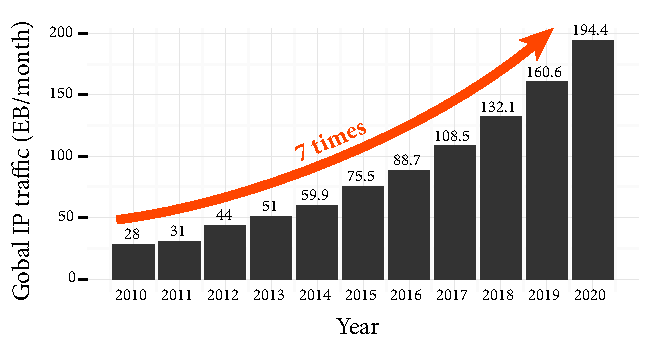
\includegraphics[width=7.5cm]{figures/vni.pdf}
    \vspace{-5pt}
    \caption{Global IP traffic~\cite{index2014forecast}.}
    \label{fig:vni}
\end{wrapfigure}
launched Amazon Snowball\index{Amazon Web Services (AWS)!Snowball}, a portable ready-to-be-shipped appliance with a storage capacity of 50~TB that can accommodate transfers of several Petabytes to \acrshort{aws}. These offloading techniques intend to overcome the challenges resulting from large-scale data transfers such as high network costs, long transfer times, and security concerns.

% As a reference, we give the duration to transfer 50~TB of data using typical Internet connections in Table~\ref{tab:truck-full-of-drives}. 
%In this thesis, we present a problem of scale. 
In this thesis, we propose to equip private vehicles with storage devices with the purpose of turning the road network into a large capacity transmission system. A back-of-the-envelope calculation shows that 10\% of the vehicles traveling the roads of France equipped with a 1~TB hard drive can transport up to 115~EB per day (1.3~PB per second). Extending this idea to the 1.2~billion cars available worldwide, the everyday mobility of vehicles represents an untapped potential for addressing the oncoming data tsunami. With data-intensive applications such as high-definition video, autonomous vehicles, and virtual reality, the demand for network bandwidth grows by an estimated 22\% per year. Already the case in some situations, in the next few years, the data consumption will outpace the network improvements made by providers in laying high-capacity fiber and speeding up their already-existing network infrastructure and servers~\cite{hecht2016bandwidth}. As shown in Figure~\ref{fig:vni}, the demand for bandwidth is at its strongest today: global \acrshort{ip} traffic has grown threefold during the past six years and is expected to double within the five next years~\cite{index2014forecast,gantz2012digital}.

The opportunistic use of vehicles follows the current trend of services that take advantage of the sharing economy (or access economy), such as BlaBlaCar and Uber, by enabling peer-to-peer-based sharing of goods and services. In our case, \textit{the trips made by the vehicles are shared resources we use to transport data on behalf of content providers}. 

Equipping vehicles with data storage also follows the second trend which consists in building value-added services right into an existing business. Examples of this trend include parcel delivery services built on top of existing passenger transportation services. In particular, Greyhound offers such a service that ``piggybacks'' on the trips made by buses as a part of the coach service.\footnote{\url{http://www.shipgreyhound.com/}} In the same manner, Uber proposes UberRUSH, an on-demand delivery service that relies on the fleet of Uber vehicles normally dedicated to passengers transportation.\footnote{\url{https://rush.uber.com}} In our case, private vehicles transport data for the account of content providers in exchange for their normal routine (\eg to synchronize backup data between remote data centers they operate). A service provider is then in charge of supervising the offloaded transfers then charged to the content providers and providing incentives to the vehicle owners for the data they transport (\eg through a ``get paid to drive'' program).
%% pourquoi pas uberEATS?

\begin{displayquote}
\textit{In this thesis, we characterize and exploit the existing mobility of everyday entities to mitigate or remove the limitations of conventional data networks. We rethink the design of popular services such as bulk data transfers or cloud-like file sharing by limiting or removing their reliance on such networks.
}\end{displayquote}
% \begin{mybox}[Vision of the thesis]{mybox:vision}
% In this thesis, we characterize and exploit the existing mobility of everyday entities to transport data for the account of large-scale services for end-to-end data transfers, storage and sharing, and vehicular resource virtualization.
% \end{mybox}


\section{Vision and data offloading design}

\begin{figure}[t]
   \centering
   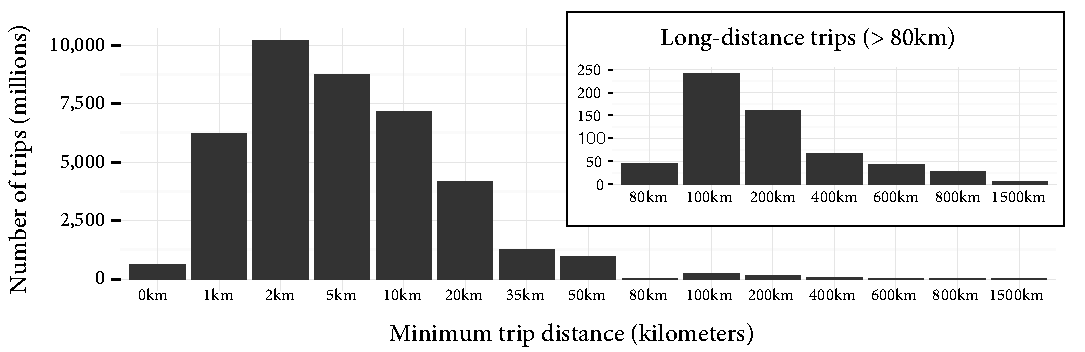
\includegraphics[width=0.9\textwidth]{figures/entd.pdf}
   \caption{Distribution of trips by distance travelled by vehicles in France. Source: the French National Household Travel Survey (ENTD), 2008~\cite{ENTD}.}
   \label{fig:entd}
\end{figure}

We exploit the \textit{delay-tolerance} of background traffic to offload bulk data transfers from a conventional data network such as the Internet over the road network. We target data transfers in the context of applications with a delay tolerance of several days (\eg distribution of large scientific datasets or traffic resulting from maintenance and provisioning activities of large-scale distributed systems)~\cite{laoutaris2009delay}. As noted by Hecht, the synchronization of the private content between remote data centers is one of the biggest drivers of bandwidth demand~\cite{hecht2016bandwidth}. Our data offloading takes opportunistic advantage of the increasing number of vehicular trips to physically transport data between locations~\cite{le2010mobilite}. 

One simple realization of the data offloading is to rely on the vehicles making the trip all the way from the source to the destination of a data transfer. However, as shown in Figure~\ref{fig:entd}, less than 1.4\% of the trips made by vehicles in France are longer than 80~km. While this number is still significant for short-distance data transfers (it corresponds to about 600 million trips per year), it becomes very low when the distance increases. Moreover, the number of destinations also increases with the distance of the trip, which results in just a few trips to transfer data over large distances. An alternative consists in using a dedicated fleet of vehicles acting as \textit{ferries} to transport the data from its source directly to its destination. However, this solution is costly and does not scale when the number of transfers increases, as more vehicles are needed to deliver the data.

Instead, we rely on dedicated facilities to \textit{compose} several flows of storage-enabled vehicles traveling in different directions. We refer to these facilities as \textit{offloading spots}\index{offloading spot} as we depict in Figure~\ref{fig:offloading-service-architecture}. Offloading spots are equipped with dedicated storage to temporarily store data and pass it between vehicles belonging to different flows. They are placed where vehicles stop often and long enough to transfer large amounts of data. Examples of such locations are on-street parking spots, garage parking, gas and electric charging stations, or supermarket parking lots. 

% When a vehicle stops at an offloading spot, the offloading spot decides whether to load or unload data based on the future direction of the vehicle. While this information may raise some privacy concerns for the driver and the passengers, we assume that it is derived from the positioning system onboard the vehicle, which provides the historical trajectories and planned itinerary to accurately predict the future direction of the vehicle~\cite{krumm2006predestination}.



%The offloading spots serve two distinct purposes, depending on their relative position in the offloading process. We represent the dual role of the offloading spots in Figure~\ref{fig:offloading-service-architecture}, in the context of a large-scale transfer of delay-tolerant data between two remote data centers. Part or all of the data originating from a conventional data network is first \textit{transloaded}\index{transloading} to the closest edge offloading spot. The data is temporarily stored at the offloading spot and is loaded onto the stopping vehicles. Subsequent intermediate offloading spots act as data relays where data is \textit{transshipped}\index{transshipping}. Vehicles drop off the data they carry while they stop at the offloading spot. The data is temporarily stored until subsequent vehicles pick it up and carry it to the next offloading spot. Once at the destination, the data is finally transloaded back into the conventional data network.

\begin{figure}[t]
    \centering
    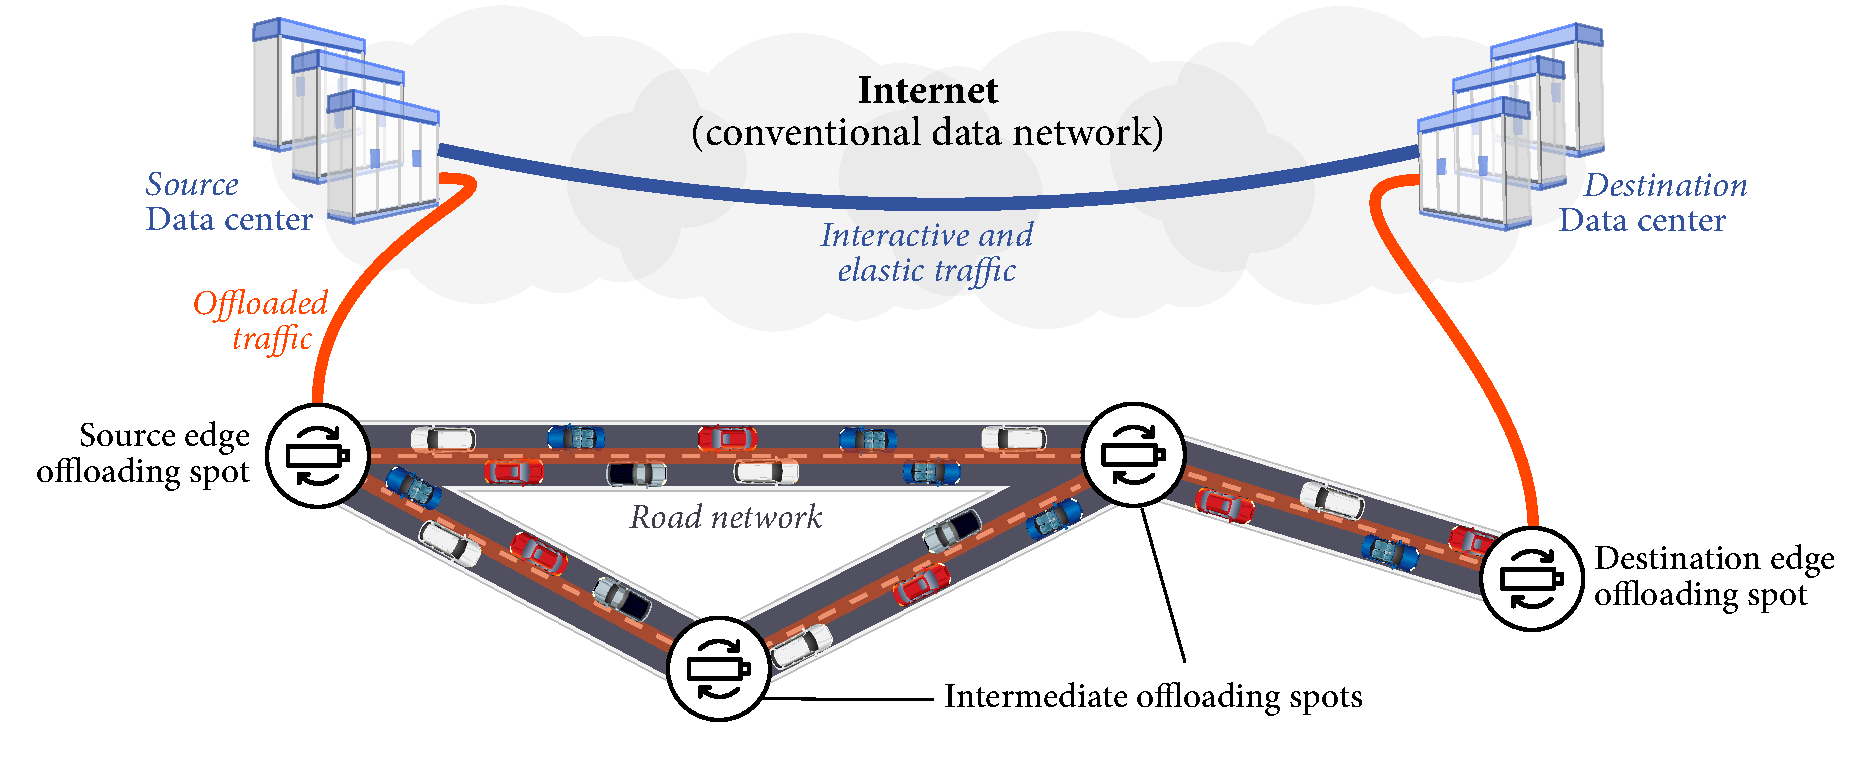
\includegraphics[width=0.9\textwidth]{figures/architecture-2.pdf}
    \caption{General overview of the data offloading we propose in this thesis.}
    \label{fig:offloading-service-architecture}
\end{figure}

% Offloading spots can also be as locations where segments of trajectories made by independent vehicles are concatenated into a single logical path followed by the offloaded data. The storing capabilities of offloading spots allow the data to be passed asynchronously from one vehicle to another. 
Following up on the work on traffic offloading, we extend the concept of offloading spot according to two distinct directions both in the context of vehicular cloud services. In the first extension, we leverage the storage capacity of the offloading spots to turn them into repositories and provide a geo-distributed system to store and share files of mobile users. To enforce the file sharing, we rely on the movements of vehicles traveling between the offloading spots to replicate the files and make them accessible to the mobile users. In the second extension, we virtualize the resources of the vehicles to create a virtual vehicular network. We dematerialize the offloading spots into pre-defined areas that feature high densities of vehicles to enable transfers of virtual machines between the vehicles. With these extensions, we further show that the existing mobility of vehicles has the potential to provide cloud services with limited reliance on conventional data networks.

% In the first extension, we leverage the storage capacity of the offloading spots to provide a cloud-like storage and sharing system for mobile users in an urban environment. The offloading spots act as repositories where users first upload their files, which are then replicated among the other repositories using the movements of the mobile users between the repositories. The replication increases the likelihood of processing the user requests to store or retrieve a file in a timely fashion.  

% In a second extension, we dematerialize the offloading spots into pre-defined areas that feature high densities of vehicles and where contacts between vehicles last long enough to transfer large amounts of data. We exploit these areas in the context of the virtualization of a vehicular network operating in an urban environment. Each vehicle hosts one or many virtual machines exploiting the abstraction provided by virtualizing the vehicle resources.
%We virtualize the resources embedded in the vehicles (\ie compute, storage, and sensing) into virtual machines. The virtualized resources are allocated to service providers, who deploy services that benefit from the movements and the shared resources of the vehicles, such as a large-scale sensing platform. 
% We show the benefits of dematerializing the offloading spots when
%and the \acrlong{v2v} communications happening in these areas 
% the migration of virtual machines is required as a result of changes in the physical topology or reallocations of the virtual resources.

%We explore \textit{how to enable efficient and reliable data transfers over the road network}. We propose an architecture that relies on a centralized controller to allow flexible and scalable configuration of the offloading spots. We use the \acrfull{sdn}\index{Software-Defined Networking (SDN)}~\cite{mckeown2008openflow} paradigm, which provides the logistics for efficient and effective vehicular transportation of data. Our \acrshort{sdn}-controlled architecture consists of a central controller\index{controller} and a collection of offloading spots. The controller receives demands to offload data transfers onto the road network. An offloading demand\index{offloading demand} indicates both the source and destination of the transfer and performance requirements, such as delay and bandwidth. The controller is then in charge of mapping the offloading demands onto sequences of offloading spots by allocating the corresponding data transfers to vehicle flows traveling between the offloading spots. 

\section{Challenges}

Firstly, we need to efficiently allocate data transfer demands to the existing flows of vehicles. We refer to this problem as the \textit{vehicle flow allocation problem}. To solve it, we need to design an efficient allocation process of the data transfers that optimizes target performance metrics, while matching the performance requirements of the corresponding demands.

\begin{wrapfigure}[13]{o}[0.7\marginparwidth]{6.2cm}
    \vspace{-15pt}
    \centering
    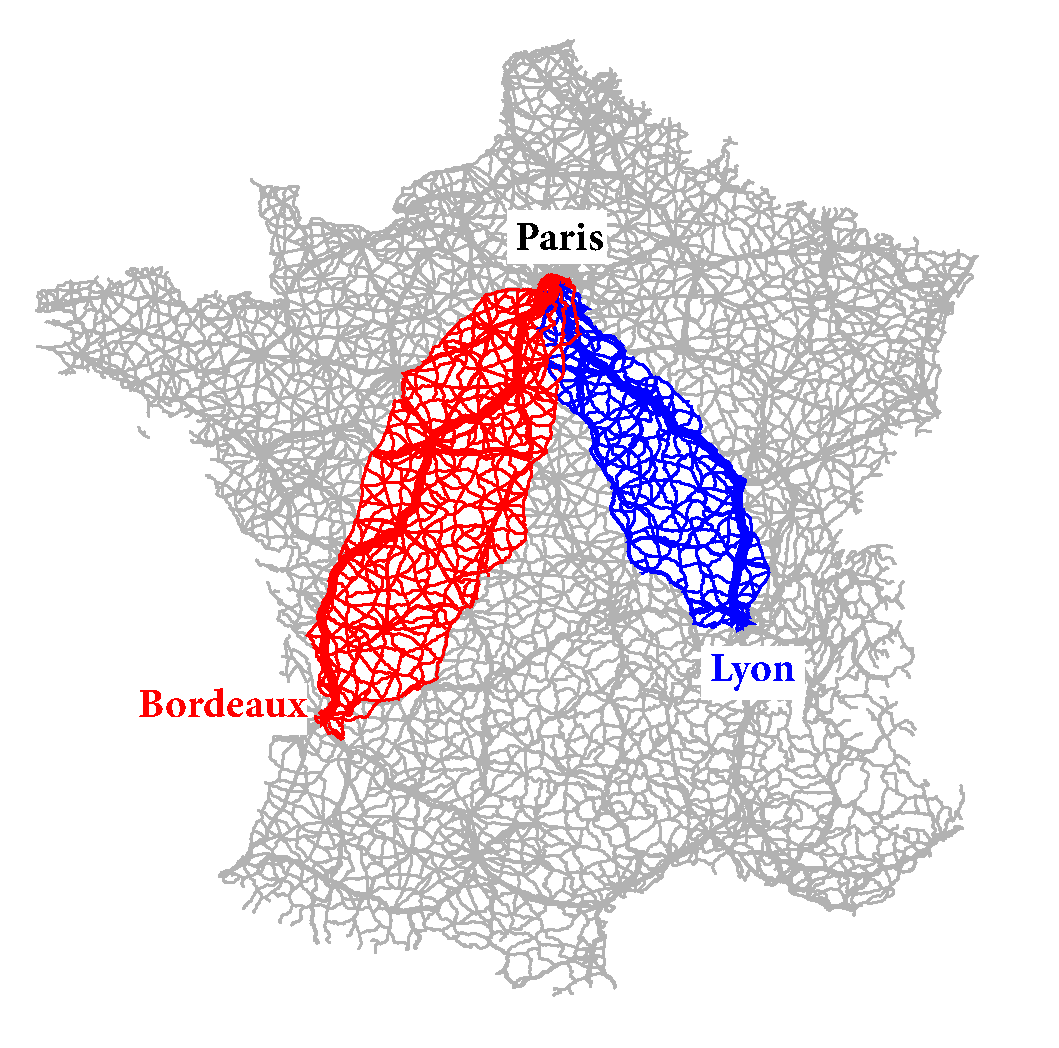
\includegraphics[width=6cm]{figures/france-roads-2.pdf}
    \caption{Main roads connecting Paris to Lyon and Bordeaux.}
    \label{fig:paris-lyon}
\end{wrapfigure}
Secondly, we need to cope with the scale of the road network in order to achieve a scalable and efficient vehicular data offloading. The complexity of the road network's topology and the large number of vehicular trips both make the vehicle flow allocation problem computationally intractable. We illustrate the need for a scalable allocation mechanism in Figure~\ref{fig:paris-lyon}, where we depict the routes of the potential trips that can be allocated to offload transfers originating from Paris to Bordeaux and Lyon. 

Finally, we need to ensure reliable data transfers. Since vehicles may fail to deliver the data they carry to the next offloading spot or the final destination, we need to rely on and adapt techniques to recover from the data losses.

In the extensions of our main work, the underlying challenge is to determine the locations of the offloading spots, whether they are materialized or not, according to the specific requirements of the services we deploy. 

In our vehicular file sharing system, we need to design an algorithm to place the repositories at strategic locations where they can capture a maximum number of user requests before they expire, while connecting them together by the movements of the users to enable the replication. In our virtual vehicular network, we need to identify the location of the areas where vehicles meet frequently and long enough to transfer large amounts of data, such as virtual machines.



\section{Contributions and thesis outline}

\paragraph{First contribution: Survey and taxonomy of techniques to transfer data using everyday mobility (Chapter~\ref{cha:state-of-the-art}).}

We begin this thesis by providing an exhaustive survey and taxonomy of the existing techniques that help exploit the mobility of everyday entities to transport data in the context of various applications. We categorize the existing techniques based on whether the delivery involves a single entity or multiple entities that take turns to transport the data. We also describe the various approaches proposed in the literature for characterizing the mobility and controlling the data forwarding.\\[3pt]
%that we use in the following chapters to achieve massive data offloading. \\
\textit{Related paper}:
\begin{itemize}
    \item Benjamin Baron, Prométhée Spathis, Marcelo Dias de Amorim, and Yannis Viniotis. ``Data transfers using everyday mobility: A survey.'' Submitted to \textit{IEEE Communications Surveys \& Tutorials}, 2016.
\end{itemize}


\paragraph{Second contribution: Assessment of the vehicular offloading concept (Chapter~\ref{cha:feasibility-study}).}

In Chapter~\ref{cha:feasibility-study}, we assess the concept of vehicular data offloading. We compare the cost of transferring data using the existing mobility of vehicles to the cost of transferring the same amount data on the Internet. We first introduce a map reduction procedure which mitigates the complexity of the road network. The output of this procedure is a logical representation which translates and characterizes the flows of vehicles into network quantities. This representation is used to solve an allocation procedure which selects the flows of vehicles in charge of carrying the offloaded data. We formulate and solve this allocation procedure as a \textit{revenue maximization model}\index{vehicle flow allocation problem!revenue maximization model} that allocates the flows of vehicles so as to maximize the cost-benefit of offloading data on the road network compared to data transfers over conventional data networks.
%We use replication techniques at the offloading spots to recover from data losses. 
Finally, we show using actual traffic counts for the French road network that our offloading concept can achieve an aggregate capacity in the Petabyte range per week.\\[3pt]
\textit{Related papers}:
\begin{itemize}
    \item Benjamin Baron, Prométhée Spathis, Hervé Rivano, and Marcelo Dias de Amorim. ``Offloading massive data onto passenger vehicles: Topology simplification and traffic assignment.'' \textit{IEEE/ACM Transactions on Networking}, 2015.
    \item Benjamin Baron, Prométhée Spathis, Hervé Rivano, and Marcelo Dias de Amorim. ``Vehicles as big data carriers: Road map space reduction and efficient data assignment.'' \textit{IEEE Vehicular Technology Conference (VTC Fall)}, 2014.
    \item Benjamin Baron, Prométhée Spathis, Hervé Rivano, and Marcelo Dias de Amorim. ``Étude de l'intermodalité pour le délestage des réseaux d'infrastructure.'' \textit{Algotel 2015~---~17èmes Rencontres Francophones sur les Aspects Algorithmiques des Télécommunications}, 2015.
\end{itemize}


% \paragraph{Second contribution: Road network logical abstraction (Chapter~\ref{cha:vehicular-offloading-service}).}

% Based on the models of the literature that characterize the mobility of the entities, we propose a reduction of the road map space into a logical overlay network. In Chapter~\ref{cha:vehicular-offloading-service}, we introduce the \textit{offloading overlay}\index{offloading overlay}, which mitigates the complexity of the road network and translates its attributes into network quantities. Together with a centralized architecture with a controller that has a holistic view of the system, it allows efficient allocation of data transfers on the road resources. We evaluate the benefits of the centralized architecture and the offloading overlay in the context of electric vehicles with a concrete deployment plan of charging stations on the French roads. \\
% \textit{Related papers}:
% \begin{itemize}
%     \item Benjamin Baron, Prométhée Spathis, Hervé Rivano, and Marcelo Dias de Amorim. ``Offloading massive data onto passenger vehicles: Topology simplification and traffic asssignment.'' \textit{IEEE/ACM Transactions on Networking}, 2015.
%     \item Benjamin Baron, Prométhée Spathis, Hervé Rivano, Marcelo Dias de Amorim, Yannis Viniotis, and Mostafa Ammar. ``Data haulage: Efficient resource management on the road network.'' Submitted to \textit{IEEE Transactions on Network and Service Management}, 2016.
% \end{itemize}


\paragraph{Third contribution: Offloading infrastructure centralized control (Chapter~\ref{chap:implementation}).}

We propose an architecture that implements the concept of vehicular data offloading. We rely on a centralized architecture that enables efficient control of the offloading infrastructure. This architecture consists of a controller and the collection of offloading spots acting as forwarding engines. The controller is in charge of selecting the road network path for each offloading demand it receives. The selection of road network paths is done so as to maximize the throughput of the resulting transfer while ensuring the fair allocation of flows of vehicles traveling the paths among the other transfers that allocated to the same paths. This is achieved by modeling and solving the allocation of a data transfer to a road path according to a max-min fairness problem\index{vehicle flow allocation problem!max-min fair allocation model}. 
%This problem that maximizes the resulting throughput while ensuring the fair allocation of the data transfers. 
%and consisting of the sequence of offloading spots. We introduce this architecture and we formulate the data transfer allocation problem as a max-min fairness allocation problem\index{data transfer allocation problem!throughput maximization model} that maximizes the resulting throughput while ensuring the fair allocation of the data transfers. 
The controller translates the output of the allocation of a data transfer by a set of forwarding rules installed at the offloading spots composing the selected road network.  Finally, the controller ensures the reliability of the offloaded data using redundancy and retransmission techniques. %to recover data lost by vehicles failing to deliver data to the next offloading spot. 
With simulations on the French road network and elaborated traffic modelling techniques presented in the Appendix~\ref{cha:traffic-forecasting-techniques}, we show that the offloading architecture we propose has the potential to offload several Petabyte of data per day.\\[3pt]
\textit{Related papers}:
\begin{itemize}
    \item Benjamin Baron, Prométhée Spathis, Hervé Rivano, Marcelo Dias de Amorim, Yannis Viniotis, and Mostafa Ammar. ``Data Haulage: Efficient resource management on the road network.'' Submitted to \textit{IEEE Transactions on Network and Service Management}, 2016.
    \item Benjamin Baron, Prométhée Spathis, Hervé Rivano, Marcelo Dias de Amorim, Yannis Viniotis, and Joseph Clarke. ``Software-defined vehicular backhaul.'' \textit{IFIP Wireless Days (WD)}, 2014.
\end{itemize}


\paragraph{Fourth contribution: Vehicular cloud services (Chapter~\ref{cha:vehicular-cloud-services}).}

We propose two extensions to the work we conduct in traffic offloading. We extend the concept of offloading spots in the context of two vehicular cloud services. A first service turns the offloading spots as repositories where mobile users can upload and share files. We propose a placement algorithm derived from the Maximal Covering Location Problem~\cite{church1974maximal} that determines the location of a target number of repositories such that (\textit{i}) a maximum of users are covered before their uploading or retrieval requests expire and such that (\textit{ii}) the synchronisation of the repositories can be done by using the existing movements of the users.

The second service virtualizes the resources of vehicles operating within a large mobile network. The offloading spots refer to specific areas where the virtual machines exploiting the abstract representation of the vehicle resources can migrate between vehicles while in contact. We propose a methodology for analyzing the spatial distribution of the contact density. This methodology determines the specific areas where contacts are long and frequent enough to accommodate the migration of virtual migrations.\\[3pt]
\textit{Related papers}:
\begin{itemize}
    \item Benjamin Baron, Miguel Campista, Prométhée Spathis, Luís Henrique MK Costa, Marcelo Dias de Amorim, Otto Carlos MB Duarte, Guy Pujolle, and Yannis Viniotis. ``Virtualizing vehicular node resources: Feasibility study of virtual machine migration.'' \textit{Elsevier Vehicular Communications}, 2016.
    \item Benjamin Baron, Prométhée Spathis, Marcelo Dias de Amorim, and Mostafa Ammar. ``Cloud storage for mobile users using pre-positioned 
    storage facilities.'' \textit{ACM SmartObjects}, 2016.
\end{itemize}

\paragraph{Thesis outline.}
This manuscript is organized in six chapters, including this introduction (Chapter~\ref{cha:introduction}). Chapter~\ref{cha:state-of-the-art} presents a review of previous approaches that propose to use mobility of entities to transport data. The two following chapters~\ref{cha:feasibility-study} and \ref{chap:implementation} present the main contribution of the thesis with, respectively, a revenue analysis and a practical implementation of the vehicular data offloading system. Chapter~\ref{cha:vehicular-cloud-services} presents two extensions of the data offloading system for vehicular cloud services. Each chapter begins with a brief introduction followed by a list of the main contributions. Given the novelty of our work, we provide additional discussions for each chapter on related topics we chose not to address in detail, including data security, privacy concerns, and road traffic dynamics. Finally, we conclude this thesis with a last chapter (Chapter~\ref{cha:conclusion}) that summarises our work and a raises futher questions as a plan for future research. 

\paragraph{Collaborations.} 
The research presented in this thesis was conducted in the context of a number of scientific collaborations: Hervé Rivano (Inria), Yannis Viniotis (NCSU and Cisco), Joe Clarke (Cisco), Miguel Campista (UFRJ), Luís Henrique MK Costa (UFRJ), Otto Duarte (UFRJ), Guy Pujolle (UPMC), and Mostafa Ammar (Georgia Tech).
\chapter[Data transfers using everyday mobility: Taxonomy and state of the art]{Data transfers using everyday mobility:\\[-5pt] Taxonomy and state of the art}
\label{cha:state-of-the-art}

The emergence of wireless capabilities equipping an ever-growing range of mobile entities has led to various paradigms such as \acrfullpl{manet}, \acrfullpl{vanet}, \acrfullpl{wsn}, and \acrfullpl{dtn}. These paradigms enable the connectivity of a wide range of mobile entities in the context of various application scenarios ranging from transportation systems to sensing platforms. 

These different scenarios exploit entities that are mobile either by nature, such as humans or animals, or by conception, like vehicles and robots moving in challenging environments. The entities are equipped with storage capabilities, allowing them to store and carry data. They are also equipped with communication interfaces to forward data when the entities come in \textit{contact}\index{contact|bb}, \ie when they are in each others' communication ranges. While most of the approaches propose forwarding strategies to cope with the mobility of the entities, we focus on those that exploit the carrying phase resulting from the movements of the mobile entities. 

% We refer to this generic architecture as \textit{intermodal}\index{Intermodal|bb}, since multiple modes of data transportation are involved to route the data to its destination. 
In this chapter, we review and provide a comprehensive categorization of the \textit{existing strategies that leverage the existing mobility of entities to physically move data}. The movements of the entities provide an alternative transmission medium, as illustrated in Figure~\ref{fig:related-work}.

\begin{figure}[h]
    \vspace{-10pt}
    \centering
    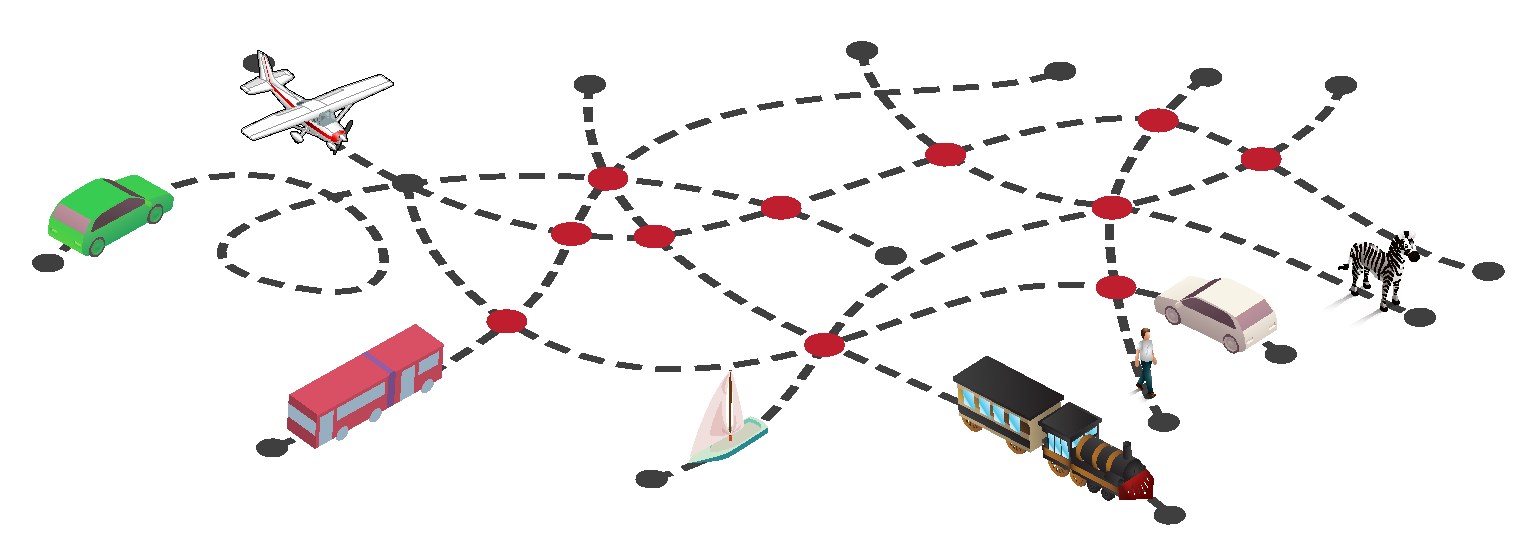
\includegraphics[width=0.55\textwidth]{figures/related-workv3.pdf}
    \vspace{-10pt}
    \caption{Alternative transmission medium based on the movements of entities.}
    \label{fig:related-work}
\end{figure}

% These entities help deliver data in environments with no infrastructure-based network available, or as a supplement or replacement to existing networks already deployed (\eg to extend their capacities). 

The idea of exploiting the mobility of different entities has been proposed in the context of various applications that do not require real-time communications. Some consider there is no data network available and entities are in charge of bringing network connectivity. Mobile entities can also be used in tandem with a conventional data network to extend the network coverage or capacity. In general, the applications rely on the following performance metrics to measure the efficiency of the data delivery:
\begin{itemize}
  \item \textit{Delivery delay}~---~the average delay to deliver the data from the sources to the destinations.
  \item \textit{Delivery rate}~---~the amount of data delivered to destinations per time unit.
  \item \textit{Delivery ratio}~---~the amount of data delivered to destinations divided by the total amount of data sent by sources that has been delivered.
  \item \textit{Energy efficiency}~---~the average amount of data delivered per unit energy consumption.
\end{itemize}  


\begin{figure}[!h]
\centering
\resizebox{\textwidth}{!}{%
\begin{tikzpicture}[every tree node/.style={align=center,anchor=north},level 1/.style={level distance=1.5cm},level 2/.style={level distance=2cm},level 3/.style={level distance=2cm}]
\Tree [.\textbf{\large Data delivery} 
        [.{\textbf{Direct} data delivery\\Single entity}
            [.\node[text width=2.5cm]{Existing mobility\\of entities}; ] 
            [.\node[text width=2.5cm]{Controlled\\entities}; ]
            [.\node[text width=2.5cm]{Delivery\\services}; ] ] 
        [.{\textbf{Indirect} data delivery\\Multiple entities} 
            [.\node[text width=3cm]{Synchronous\\composition}; 
                [.\node[text width=3cm]{Pre-positioned\\composition}; ]
                [.\node[text width=3cm]{Floating\\composition}; ] ] 
            [.\node[text width=3cm]{Asynchronous\\composition}; 
                [.\node[text width=3cm]{Pre-positioned\\composition}; ]
                [.\node[text width=3cm]{Floating\\composition}; ] ] ] ]
\end{tikzpicture}}
\caption{Classification of the trajectory composition according to the type of data delivery.}
\label{fig:classification-survey}
\end{figure}

We represent the structure of the classification in Figure~\ref{fig:classification-survey}. Some works propose the use of a single entity to carry the data from its source all the way to the final destination. This results in a \textit{direct data delivery}, which we present in Section~\ref{sec:direct-delivery}. However, relying on a single entity is somehow limiting from the perspective of the expected benefits (\eg capacity or coverage). The idea of composing the trajectories of multiple mobile entities was thus introduced. According to this idea, the data follows a path consisting of multiple segments of trajectories, each followed by different mobile entities. This results in an \textit{indirect data delivery}, which we present in Section~\ref{sec:indirect-delivery}. Data is passed from one entity to another as a result of the forwarding when entities are in direct contact.

In the case of indirect data delivery, we choose to present the works that are the most relevant to this thesis. They propose different strategies for composing the trajectories of mobile entities. These strategies differ depending on the two following criteria:

\begin{itemize}
  
    \item The \textit{time} when composition should occur. The data is passed either \textit{synchronously} when two entities meet or buffered before passed \textit{asynchronously} to subsequent entities.  

    \item The \textit{location} where composition is performed. The location can be either \textit{pre-defined} or \textit{floating}. In the pre-defined case, the data is passed if the entities are in contact at specific locations. In the floating case, composition results of contacts between entities regardless where they are in contact.

\end{itemize}

The strategies proposed in the literature result of the combination of one of the instances of both previous criteria. 

% The simplest approach consists in using the movement of a single entity to eventually make the entire trip between the source(s) and the destination(s) of a data transfer. This approach is generally referred to as ``Direct delivery''\index{Direct delivery}. However, there are no guarantees on the actual delivery of data, as the movements of the entity are difficult to predict and do not necessarily match the source(s) and destination(s) of the data transfer. As a result, one entity is not enough to provide robust and reliable data transfers.

% Instead of using a single entity, \textit{concatenating} the movements of multiple entities to transport the data offers multiple paths to route the data, allowing to improve network performance (\eg delivery delay or ratio). The entities relay each other to transport the data from its source(s) to its destination(s) along a logical path and resulting in an indirect delivery. The concatenation of the movements corresponds to encounters between two entities when in each other's transmission range, that is when they are in \textit{contact}. They are the result of the opportunities to forward data when two entities come in contact. As a result, multiple concatenations of the movements of the entities are possible and their selection depends on the performance metrics to optimize. The movement concatenations are either synchronous or asynchronous, depending whether the entities directly forward the data or forward it via intermediate nodes. Synchronous concatenations are subjected to contacts, which that can happen anywhere between any two entities. They result from the decisions to either forward, replicate or keep the data. Conversely, asynchronous concatenations are the result of remote contacts between entities via intermediate nodes. The placement of stationary intermediate nodes or the movement of mobile ones induce the remote contacts between entities. Despite their uncontrollable movements, some entities share mobility patterns with common characteristics and concentrate in specific regions (\eg intersections in the case of vehicles). Since these regions have a high concentration of entities, they are more likely to encounter each other, creating potential concatenations of their movements. In this context, synchronous concatenation approaches benefit from the spatial distribution of the entities to geographically anchor the concatenation of their movements at specific locations with high entity concentrations. In the case of asynchronous concatenation, these locations correspond to the location of the stationary dedicated nodes.  

% In the following, we review both the direct and indirect delivery approaches.

% The contacts create opportunities to forward, resulting in different ways to concatenate the movements of the entities depending on the performance metrics to optimize.

% The entities can use this contact as an opportunity to forward the data they carry to one another. Indirect delivery approaches exploit the combination of the movements according to temporal and spatial dimensions. As contacts require encounters at the same time and location, the combination of movements is \textit{synchronous}. Conversely, approaches leverage dedicated nodes, either mobile or stationary to combine the movements of different entities in an \textit{asynchronous} manner. While the combination of the movements can happen anywhere, some approaches benefit from the spatial distribution of the entities to geographically anchor the combination of the movements of the entities at specific locations with high entity concentrations. In the case of asynchronous combination, these locations correspond to the location of the stationary dedicated nodes. 


\section{Direct data delivery}
\label{sec:direct-delivery}

In this section, we present the direct delivery strategies that exploit the movements of a single entity to carry data. We classify these strategies according to the degree of knowledge regarding the mobility of the carrying entity. 

Firstly, we consider the strategies using entities exhibiting random mobility. Although they eventually deliver the data they carry, the delivery delay can be excessively long, making the transfers unreliable and unfit for real-life applications. 

Having partial knowledge about the movements of the entities allows the deployment of applications that require performance guarantees, such as sensing platforms and systems to extend the connectivity of remote areas. 

Secondly, we consider the entities whose mobility is pre-calculated in advance. The related strategies and the related approaches to control their movements to transport the data. Controlling the movements of the entities provides better guarantees on the delivery delay and rate, which matches the requirements of sensing applications. 

Finally, we review the approaches that leverage third-party services such as postal services to transport data. These services allow the transfer of large amounts of data, resulting in a large capacity alternative medium for large-scale bulk data transfers.

\subsection{Existing mobility of entities}
\label{sec:direct-non-control}

\begin{wrapfigure}[11]{o}[0.7\marginparwidth]{5.5cm}
    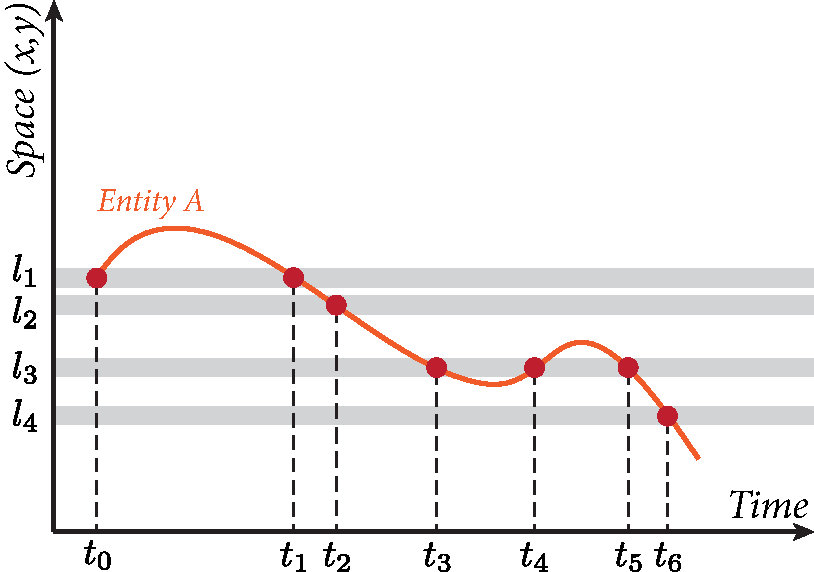
\includegraphics[width=5.3cm]{figures/dtn-direct-forwarding.pdf}
    \caption{Direct delivery using the existing movements of a single entity.}
    \label{fig:dtn-direct-forwarding}
\end{wrapfigure}
Several approaches rely on the existing movements of a single entity to transport the data in the context of delay-tolerant applications such as sensing platforms or periodic data transfers to bridge connectivity gaps in remote areas not covered by conventional data networks. The data is loaded in the storage of the mobile entity when it comes close to the source (\eg sensor nodes or gateway connected to a data network). As represented in Figure~\ref{fig:dtn-direct-forwarding}, the entity transports the data as part of its usual movements and unloads the data when it comes close to the destination (\eg sensor sink or gateway). Since only one copy of the data is carried, this approach does not consume many resources and has a minimum overhead. With no knowledge on the mobility of the entity, there are no guarantees on the expected delivery, which makes this strategy highly unreliable. However, some approaches exploit the knowledge of the mobility of the entity to deploy applications with stronger performance guarantees.

\paragraph{Random entity mobility.}
In the case of a random mobility, Grossglauer and Tse show how to use entities with unknown mobility to transport data instead of using traditional ad hoc networks where a wireless multi-hop path must always exist between the source and the destination~\cite{grossglauser2001mobility}. The direct delivery approach leads to better throughputs under large data loads compared to the ad hoc case, as most of the traffic carried by the entities in ad hoc networks is relayed traffic, which consumes both energy and bandwidth. However, using the mobility of the entities leads to high delays, as the entity carrying the data may take a long time before coming in contact with the destination. 

\paragraph{Large-scale sensing platforms.}
Large-scale sensing platforms can benefit from the random movements of entities to collect data from sensors scattered in an area, or even generate environmental data as part of their movements when equipped with sensors. The data is temporarily stored and carried by the entities and delivered to a central sensor sink when the entity moves close. The sensor sink aggregates the data to transfer it to remote servers using a conventional data network for long-term storage and analysis. Compared to ad hoc networks, this transmission model allows large power savings and higher bandwidth at the sensor nodes because the communications take place over short ranges, which reduces the power of the radios. 

Burrell~\etal study the deployment of sensor networks in vineyards to take effective decisions in the face of low temperatures, rain or frost. The authors relied on vineyard workers to transport the data from the sensors to the sink located in the farm~\cite{burrell2004vineyard}. SeNDT (Sensor Networking with Delay Tolerance) is a system for water pollution and noise monitoring at a lake in the center of the Republic of Ireland, which relies on sensors deployed around the lake~\cite{mcdonald2007sensor}. To collect the data, the authors mounted wireless devices on anglers' boats that they use to fish in the lake to collect sensor data as part of their movements on the lake. The data is then aggregated at a sink in the boathouse when the anglers return. The EMMA project aims at monitoring pollution using buses to generate location-based environmental data along their movements~\cite{lahde2007practical}. As part of their routes, the buses transport the data to stationary sinks placed in strategic locations, such as intersections. Using the existing movements of entities as part of sensing platforms to generate or collect sensing data avoids costly deployments to transmit the data through intermediate nodes and increases the lifetime of the sensor nodes by using short-range radios. However, such platforms must have loose constraints on the delivery rate and delay of the data as they rely on unpredictable movements of the entities.

With knowledge on the mobility patterns of the entities, DakNet leverages the bus schedules to provide Internet connectivity to remote regions of India and Cambodia~\cite{pentland2004daknet}. Equipped with mobile access points, the buses physically transport the data between Internet access points located in larger cities and rural kiosks located in the villages to exchange delay-tolerant data such as mail or land records. This provides an efficient low-cost alternative to expensive dialup 
\begin{wrapfigure}[9]{o}[0.7\marginparwidth]{5cm}
    \vspace{-10pt}
    \includegraphics[width=4.9cm]{figures/pigeon.jpg}
    \caption{A pigeon equipped with a backpack carrying an SD card.}
    \label{fig:pigeon}
\end{wrapfigure}
landlines or long-range radios. Compared to the previous approach, DakNet gives better guarantees because of the fixed schedule of the buses. A similar initiative was proposed by the Wizzy Digital Courier service to provide connectivity to access schools located in remote villages of South Africa~\cite{rabagliati2004wizzy}.

RFC 1149 specifies an experimental method to transmit IP datagrams using avian carriers, as represented in Figure~\ref{fig:pigeon}~\cite{rfc1149}. Although suited for very specific scenarios, this solution becomes infeasible in large-scale networks due to the high delay and low throughput of the transfer. Some implementations of the protocol lead to large losses (with over 55\% of lost datagrams) and variable delays of several hours when transporting the data over five kilometers.

While the endpoints of the pigeon route are pre-defined, its movements are random and lead to losses, making the transfer unreliable and unsuitable for the targeted applications. In the following, we overview the different approaches that leverage controllable entities to provide reliable data transport.

\clearpage
\subsection{Controlled entities}
\label{sec:direct-control}

\begin{wrapfigure}[11]{o}[0.7\marginparwidth]{5.5cm}
    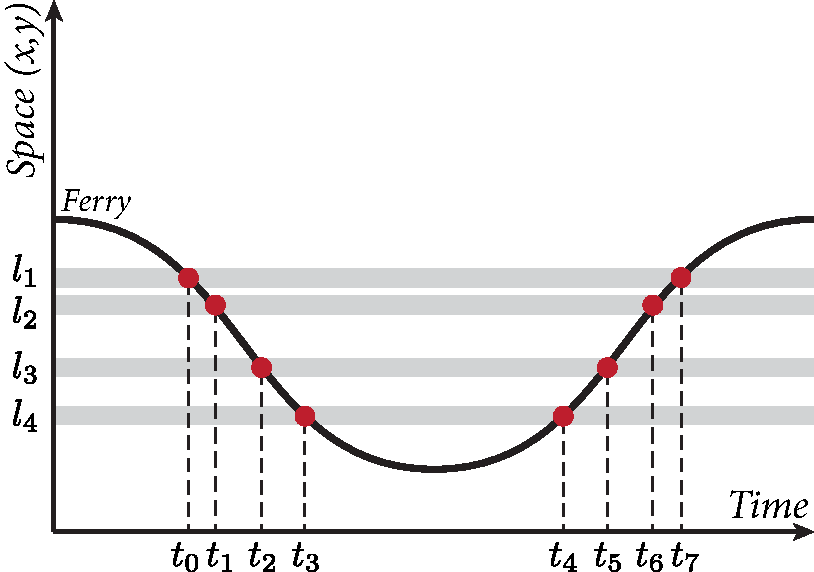
\includegraphics[width=5.3cm]{figures/dtn-direct-controlled-forwarding.pdf}
    \caption{Direct data delivery with a controllable entity.}
    \label{fig:dtn-direct-controlled-forwarding}
\end{wrapfigure}
Contrary to using the existing movements of entities, controlling their movements provides better performance guarantees, for instance on the delivery rate and delay of the data. Generally referred as ``ferries'' or ``robots'', these dedicated entities are generally used in sensor networks to provide communication capacity among the sensor nodes by picking up data from the source(s) and carrying it to the destination(s), as depicted in Figure~\ref{fig:dtn-direct-controlled-forwarding}. In this figure, a ferry periodically visit the nodes located at $l_1$, $l_2$, $l_3$, and $l_4$. An underlying challenge is to compute a route for the dedicated entity such that it visits all the nodes and optimizes performance metrics (\eg average delivery delay and rate). In the work we review, the nodes generate data traffic (uniform or not), which results in different bandwidth requirements that the dedicated entity has to satisfy. Otherwise, the data generated at the nodes accumulates to a point where it is dropped in case of limited buffer capacity.

\paragraph{Message ferry.}
In the initial message ferry work, Zhao \etal proposed an algorithm to compute the ferry route of a single ferry such that it minimizes the average delivery delay of the data generated uniformly by a collection of stationary nodes~\cite{zhao2003message}. The algorithm first creates a route using local optimization techniques for the \acrfull{tsp} (2H-opt) that minimizes the average delay for all traffic generated by the nodes. Second, the algorithm extends the original route to meet the bandwidth requirements of the nodes. While this technique works well with equal node bandwidth requirements, it does not adapt to unequal ones. 

\paragraph{Unequal bandwidth requirements at the entities.}
With unequal bandwidth requirements, Mansy \etal propose to use the deficit round-robin technique to decide which node to visit next depending on the visit history and the last meeting with the ferry~\cite{mansy2011deficit}. With this approach, nodes with higher data rates get better chances to be visited by the ferry. Tirta \etal propose to decrease the delay of the ferry route by visiting fewer nodes using the ad hoc connectivity of the nodes to form clusters~\cite{tirta2004efficient}. The ferry only visits one node per cluster, the \textit{cluster head}, which aggregates and distributes the data from and to the other nodes of the cluster. The authors focus on the impact of different route schedules on the buffer size of the cluster head, which sees a large load of messages to aggregate and distribute. The authors show that scheduling the visits of the ferry to minimizing its movements reduces the energy consumption of the ferry. However, scheduling the visits of the ferry at the cluster heads according to the data rate aggregated at the cluster heads leads to better delivery delays.

\paragraph{Multiple controllable entities.}
Adding more controllable entities to collect the data of the nodes increases the cost, but also improves the network capacity and overall performance, as the entities can cover larger distances, handle more traffic load, and provide better reliability in case of failure. Zhao \etal propose two different techniques to directly deliver data among the nodes using multiple message ferries~\cite{zhao2005controlling}. The first technique consists in designing a single route using the same heuristic as followed by all the ferries with the same speed and different timings, allowing each node to communicate with all the ferries~\cite{zhao2003message}. The second technique is more complex and consists in designing multiple routes followed by the ferries instead of a single route. Since the data is not relayed by the ferries, each route must accommodate all the bandwidth requirements of the node visited by the ferry on the route. The authors propose a greedy heuristic that assigns nodes to ferries and balances the traffic load among the routes by shortening or extending them such that the estimated weighted delay of the data traffic among the nodes is minimized. 

More recently, pigeon networks introduced \textit{pigeons} that act as ferries between a ``home host'' and ``foreign hosts'' on dedicated routes~\cite{zhou2013minimizing}. There are no data exchanges between the ferries, so each route must accommodate the requirements of every foreign host they visit. The authors propose an exact optimization technique to design the routes of the pigeons such that they minimizes the average delay of the generated data. This technique is optimal for small-scale networks but becomes intractable for larger networks. To make the problem tractable, they propose a geographical partitioning-based heuristic that relies on the divide-and-conquer idea to design the pigeon route. The authors show that the resulting route yields lower delays compared to the non-partitioning strategy used in the route design of the message ferry work.

\paragraph{Real-world deployments.}
Several projects have studied and deployed controllable entities in real-life settings in the context of sensing platforms. Tekdas~\etal deployed a small sensor network with robots to measure the energy savings brought by the addition of the robots~\cite{tekdas2009using}. With robots assigned to different routes using the $k$-\acrshort{tsp} heuristic, which finds $k$ tours where the largest of the $k$ tours is minimized, they showed significant energy savings at the sensor nodes from 1mW in tradition ad hoc to 0.003mW with the robots. Since the robots come close to the sensor nodes, they require limited transmission power and fewer transmission attempts, which decreases the overall energy consumption. 

\paragraph{Underwater networks.}
Underwater networks of sensors deployed in the oceans for long-term environmental monitoring or surveillance also leverage robots to collect sensor data~\cite{partan2007survey,akyildiz2005underwater,dunbabin2006data}. Because of the cost of the underwater sensor nodes and the extent of the areas to monitor, the deployment of underwater sensor networks is generally sparse, making it impossible to form an unpartitioned ad hoc network. Robots or \acrfullpl{auv} transport sensor data between the sensor nodes in the partitions. These networks differ from terrestrial sensor networks because of the acoustic channel shared between the communications among the sensors and the \acrshortpl{auv}, and the navigation system of the \acrshortpl{auv}. This twofold utilization of the medium creates contentions, limiting its use. The \acrshortpl{auv} use visual odometry to travel to the next sensor node and collect its data. The \acrshortpl{auv} then send via a high-bitrate channel the data collected from the underwater sensors to buoys acting as sinks.

Using controllable entities to enable the communication between static nodes gives better delivery delays and rates, as the route followed by the entity is specifically designed to optimize these metrics. In the following, we review the approaches that use existing delivery services to transport the data instead of controlling the mobility of entities. These approaches rely on entities already operated and managed by the delivery services.

\subsection{Delivery services}
\label{sec:thrid-party-services}

% Contrary to the previous approaches that target sensing platforms or remote transfers to bridge the connectivity gap between remote regions, the approaches we review here leverage third-parties to transport data. Commonly referred as \textit{SneakerNet}\index{SneakerNet|bb}~\cite{patterson2003conversation}, these approaches control the endpoints of the data transfers. They create an alternative transmission medium to offload data from infrastructure-based networks. Offloading was used during the Cold War by diplomats to exchange suitcases with one-time pads printed on tapes to encode the real-time communications between Washington and Moscow~\cite{kahn1974codebreakers}. While offloading can create a secure channel, it also has a high bandwidth potential, as stated by Andrew Tanenbaum\index{Tanenbaum|bb}~\cite{tanenbaum2003computer}:
% \begin{quote}
%     \textit{Never underestimate the bandwidth of a station wagon full of tapes hurtling down the highway.}
% \end{quote}

\begin{wrapfigure}[10]{o}[0.7\marginparwidth]{5.5cm}
    \vspace{-10pt}
    \centering
    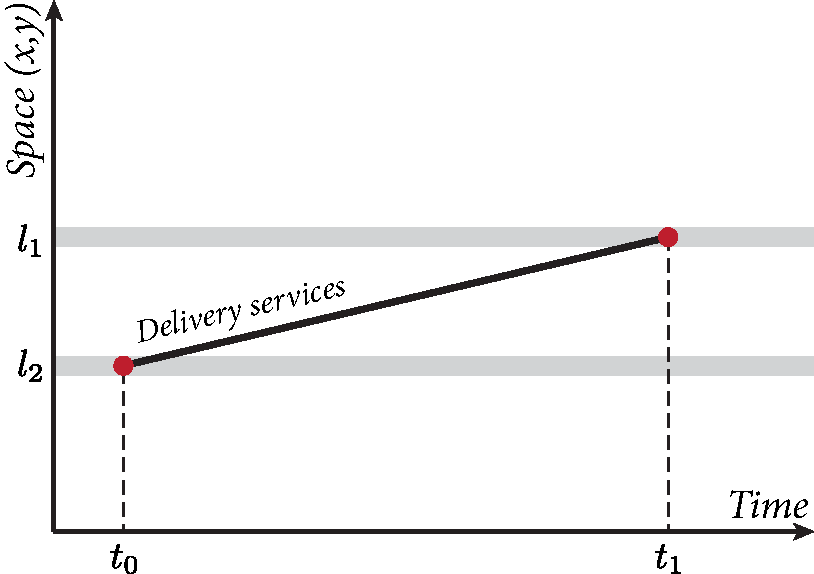
\includegraphics[width=5.3cm]{figures/dtn-direct-delivery.pdf}
    \caption{Direct data delivery using delivery services.}
    \label{fig:dtn-direct-delivery}
\end{wrapfigure}
Delivery services (\eg USPS, La Poste, FedEx, or UPS) provide an alternative mean to transport data by shipping hard drives and disks over long distances, as they avoid deploying and maintaining costly conventional data networks. Delivery services target delay-tolerant transfers and provide guarantees on the delivery date and shipping cost of the parcels. We represent their use in Figure~\ref{fig:dtn-direct-delivery} where the data is transported from location $l_1$ to location $l_2$.

Wang~\etal proposed Postmanet, a generic system that complements the Internet and provides connectivity to areas in rural regions using postal services~\cite{wang2004turning}. The data is copied on DVDs and shipped in parcels to remote Postmanet routers that act as gateways similar to rural kiosks, which, in turn, put the received data at disposal to the remote users (\eg email or land records). The authors overview different routing strategies to ship the data, including direct shipping between users. Since the other strategies rely on intermediate servers to dispatch the data, we will review them in Section~\ref{sec:indirect-async-anchored} where we review the indirect delivery approaches. 

\begin{wrapfigure}[9]{o}[0.7\marginparwidth]{4.4cm}
    \centering
    \vspace{-15pt}
    \includegraphics[width=3cm]{figures/Snowball.png}
    \caption{Amazon Snowball.\index{Amazon Web Services (AWS)!Snowball}}
    \label{fig:snowball}
\end{wrapfigure}
Laoutaris~\etal compared the cost of sending data using postal services with the cost of sending the same amount of data through a conventional data network, as content providers operating several datacenters would do~\cite{laoutaris2009delay,laoutaris2013delay}. Such data transfers are currently serviced by expensive dedicated networks (\eg Large Hardon Collider Computing Grid) or by postal services. The authors exploit intermediary storage in transit \acrfullpl{isp} to temporarily buffer the data and send it during off-peak hours when the costs to transmit data are low. The authors found that it is less expensive to use the postal services for individual shipments that occasionally happen (\eg short-lived transfers). However, in the case of a constant flow of data to transfer, they show that shipping data is more expensive than sending it through an \acrshort{isp} using the intermediate storage the authors propose to use.

\paragraph{Commercial applications using delivery services.}
Many commercial applications rely on postal services to exchange content with their customers. As an example, Netflix\index{Netflix} offers a DVD rental service to its customers\footnote{\url{http://dvd.netflix.com/}} which allows them to rent DVDs and receive them in the mail. Netflix' customers may keep a DVD as long as they want, and must return it before renting another DVD. With this service, Netflix currently distributes more than 1.5~million DVDs a day\footnote{\url{ http://ir.netflix.com}}, accounting for a total aggregate bandwidth of more than 650 Gbps. 
% http://files.shareholder.com/downloads/NFLX/182838532x0x102020/5a5dc220-6f8b-4704-a380-2c81a3a37958/factsheet.pdf

Large cloud providers offer services to allow their customers to ship physical media of their data to be uploaded to remote cloud storage (\eg
\acrshort{aws} Import/Export\index{Amazon Web Services (AWS)!Import/Export}\footnote{\url{http://aws.amazon.com/importexport}}, 
Microsoft Import/Export Service\footnote{\url{http://azure.microsoft.com/en-us/documentation/articles/storage-import-export-service/}} and more recently 
Google Offline Disk Import\footnote{\url{https://cloud.google.com/storage/docs/offline-media-import-export}}). AWS launched the Amazon Snowball\index{Amazon Web Services (AWS)!Snowball} (shown in Figure~\ref{fig:snowball}) is a portable ready-to-be-shipped appliance with a storage capacity of 50~TB that aims to accommodate transfers of several Petabytes (using multiple Snowball) to \acrshort{aws} servers. Amazon compares this solution with transfers on common Internet connections and shows that it takes approximately a week to transfer 50~TB via a 1G connection, or to ship a  Snowball with the same amount of data. Therefore, this solution exemplifies the potential of physically transferring data for massive data offloading.

% With this appliance, Amazon customers trade speed for money, as renting a Snowball costs \$200 plus the shipping costs. Comparatively, leasing a dedicated line from a Tier 1 ISP (\eg Level 3) costs about \$1~-~\$2 per Mbps for a 10G port, which rounds up to \$10,000 for a fully utilized 10G port (including collocation and equipment leasing costs)\footnote{\url{http://drpeering.net/white-papers/Internet-Transit-Pricing-Historical-And-Projected.php}}. Therefore, as noted by Laoutaris \etal~\cite{laoutaris2009delay}, leasing an Amazon Snowball for a single transfer is more profitable than leasing a dedicated line for similar resulting bandwidth.

% \begin{table}[h]
%     \centering
%     \begin{tabular}{|c|c|c|c|c|}
%         \hline
%          & \multicolumn{4}{c|}{Internet connection speed} \\
%         \hline
%         Utilization & 1Gbps & 500Mbps & 300Mbps & 150Mbps\\
%         \hline
%         25\% & 19 & 38 & 63 & 126 \\
%         \hline
%         50\% & 9 & 19 & 32 & 63 \\
%         \hline
%         75\% & 6 & 13 & 21 & 42 \\
%         \hline
%     \end{tabular}
%     \caption{\textit{How fast is that truck full of drives?}~---~Numbers of days to transfer 50~TB via the Internet at typical utilizations. The table appeared on slides from Amazon Web Services.} 
%     % \footnote{\url{http://www.slideshare.net/AmazonWebServices/aws-october-webinar-series-introducing-aws-import-export-snowball}}.}
%     \label{tab:truck-full-of-drives}
% \end{table}


\section{Indirect data delivery}
\label{sec:indirect-delivery}

As we have seen in the previous section, relying on the existing movements of a single entity to transport the data limits the expected performance of the resulting transfers, in terms of the delivery delay and rate. Instead of one entity, one can \textit{compose} the trajectories of multiple entities to transport the data to its destination. Composing the trajectories of entities gives the opportunity to route the data on multiple paths, thus increasing the resulting capacity and reliability of the data transfers. As we have mentioned in the introduction of this chapter, we classify the different strategies for composing the trajectories of entities depending on the time and location of the composition. 

Firstly, we review the strategies that rely on the synchronous composition of the trajectories of entities. In this case, the data is then passed from one entity to another whenever two entities come in contact. The different strategies we review propose more of less elaborated control planes to decide whether to forward, replicate, or keep the data during a contact to optimize the performance of the resulting data transfers.

Secondly, we review the strategies that rely on a dedicated infrastructure that consists of either stationary or mobile nodes with controlled mobility to asynchronously compose the trajectories of the entities. This infrastructure mitigates the effects of the partial knowledge of the movements of the entities and allows efficient compositions of the movements to improve the performance of the data transfers, in terms of delivery delay and rate. 

% This combination can be synchronous or not and can happen at specific locations or not. The data is then relayed from one entity to another whenever two entities encounter or come in contact with each other's transmission range. When in contact, the entities decide whether to forward the data or not to the other entity. The entities may also decide to replicate the data, thus increasing the number of possible paths to the destination. While replication seems appealing to increase the chances to deliver the data in less time, it requires more node resources (\eg storage and energy) to buffer and transmit the additional copies of the data. However, these decisions are difficult to make when the mobility of the entities is not well-known. Approaches proposed to introduce non-randomness by deploying a dedicated infrastructure to support the data transport. This infrastructure consists of mobile or stationary nodes that \textit{asynchronously} relay the data between entities. In this section, we review the different approaches that leverage synchronous forwarding between entities in contact and asynchronous forwarding with support infrastructure.

\subsection{Synchronous composition of the trajectories}
\label{sec:indirect-sync}

If the data is passed in a synchronous way, the two mobile entities involved in the composition of their trajectories are required to be in contact at the same time. As a result, the data follows a route that consists of the successive compositions of the trajectories of the entities that physically carry the data towards its destination. This approach is commonly referred to as \textit{mobility-assisted forwarding}, or also as \textit{store-carry-and-forward}. The work we review in this section proposes different control plane approaches to make the forwarding decisions over contacts. Instead of using straightforward decisions based on a local control plane, the approaches that leverage a global control plane make more informed and efficient forwarding decisions to improve the performance of the data transfers. 

While the contacts can occur anywhere, only few should be considered to compose the trajectories of the entities. Some strategies only consider the compositions that result of the contacts occurring in specific pre-defined areas. These areas correspond to locations with higher densities of entities with more contact opportunities than the other locations with lower densities. Routing data between these areas enables better control of the forwarding and requires fewer replications to deliver the data.

In the following, we present the strategies that transfer the data over synchronous compositions of the trajectories of entities either with floating compositions or at pre-defined locations.

% With synchronous combinations, the data follows a route that results from the successive combinations of the movements of the entities that physically carry the data towards its destination. This approach is commonly referred to as \textit{mobility-assisted forwarding}, or also as \textit{store-carry-and-forward}. The work we review in this section proposes different control plane approaches to make the forwarding decisions over contacts. Instead of using straightforward decisions based on a local control plane\index{Control plane}, the approaches that leverage a global control plane make more informed and efficient forwarding decisions, thus enhancing the network performance. With a global control plane, some approaches restrict the forwarding decisions to geo-anchored locations with higher densities of entities. Having more concentrated contact opportunities increases the chances to make the right forwarding decisions. In a first part, we review the approaches that do not restrict the forwarding decisions to any specific locations and in a second part, we review the approaches that leverage forwarding decisions geo-anchored at specific locations.


\subsubsection{Floating composition}
\label{sec:indirect-sync-non-anchored}
% DTN routing

\begin{wrapfigure}[10]{o}[0.7\marginparwidth]{5.5cm}
    \vspace{-10pt}
    \centering
    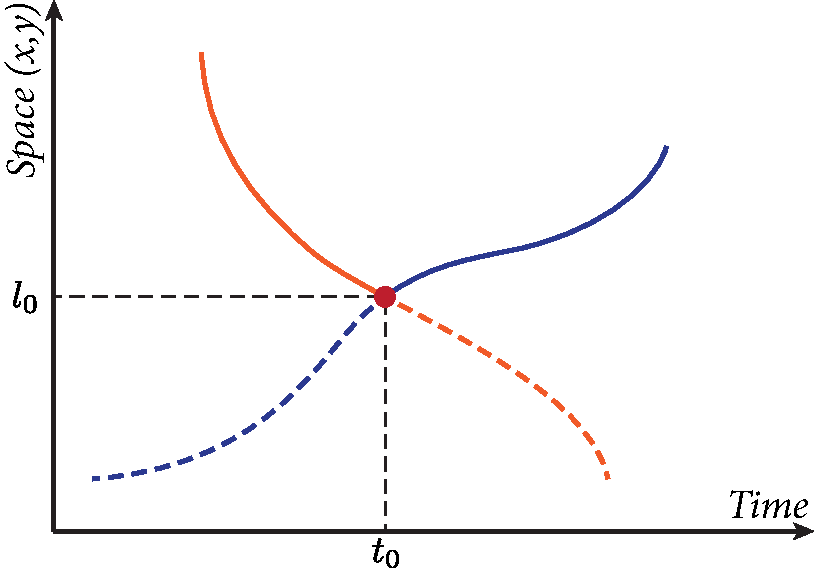
\includegraphics[width=5.3cm]{figures/dtn-indirect-sync-nongeo.pdf}
    \caption{Indirect synchronous floating composition between two entities.}
    \label{fig:dtn-indirect-sync-nongeo}
\end{wrapfigure}
When two entities come in contact at the same time and location, it creates an opportunity to compose their trajectories and bring the data closer (in time) to its destination. We represent the floating composition in Figure~\ref{fig:dtn-indirect-sync-nongeo} where the data is passed from entity $B$ to entity $A$. During a contact, the two entities can forward, replicate, or keep the data they carry. In this section, we review the different strategies to synchronously compose the trajectories of entities. The applications envisaged with these strategies must tolerate delayed deliveries. They range from sensor networks to vehicular networks and battlefield communications.

\paragraph{No control plane.}
With no control plane, the entities compose their trajectories with any other entities they encounter by replicating the data they carry. This is how the epidemic protocol works by disseminating the data~\cite{vahdat2000epidemic}. Every intermediate entity that receives the data replicates it to all its neighbors and so on. With this approach, the data is certain to be delivered with the minimum delay at its destination, as one of the copies follows the shortest route between the source and the destination. However, under limited resources, including buffer storage, this strategy is not efficient as it creates an exponential number of copies of the data and fills the buffers of the entities.

Originally proposed in the context of sensing platforms, the data \acrshort{mule} architecture leverages the movements of entities to collect data from sensors scattered in a sparse area and deliver it to access points~\cite{shah2003data}. To improve the system performance, the \acrshortpl{mule} can communicate with each other to either form an ad hoc multi-hop \acrshort{mule} network or to compose their movements and disseminate the data when in contact. CarTel~\cite{hull2006cartel} and BikeNet~\cite{eisenman2009bikenet} have both implemented the data \acrshort{mule} architecture to generate sensing data using sensors mounted on vehicles and bikes equipped with sensors, respectively. Note that, in both works, the dissemination protocol was not implemented and was instead replaced by a direct delivery approach.

The Infostation model presents a data \acrshort{mule} application where mobile entities connect to Infostations that act as access points distributed over a geographical area~\cite{goodman1997infostations}. When in the vicinity of an Infostation, the entities transmit at very high rates, thus trading connectivity for capacity. With the Shared Wireless Infostation Model, Small and Haas enhanced the Infostation model with the epidemic routing in the context of whale monitoring with radio-tagged whales that continuously collect biological and environmental data~\cite{small2003shared}. The data collected by the whales is then transmitted when the whales surface to buoys that act as Infostations. The epidemic protocol is used to exchange monitoring data when the whales are grouped together. Since the epidemic protocol generates a large number of replicas, the data accumulates at the buffers, resulting in buffer overflows and data drops. To limit the number of copies of the same file in the network, the authors use an infectious disease model that ``infects'' the whale with a data according to a given probability, if not already infected. This probability is chosen such that it is equal to the probability that the data will be offloaded within a target duration since its generation. 

\paragraph{Maintaining a local control plane.}
Subsequent approaches proposed a local control plane to improve the performance epidemic protocol and limit the excessive usage of the resources. The Spray-and-Wait protocol bounds the number of copies to send per data using two phases~\cite{spyropoulos2005spray}. In the ``spray'' phase, a given number of copies are transmitted from the source to other entities that act as relays. In ``wait'' phase, the relays with a copy of the data wait to encounter the destination of the data. The Spray-and-Focus protocol~\cite{spyropoulos2007spray} uses the same ``spray'' phase as~\cite{spyropoulos2005spray}, followed by a ``focus'' phase where the copies can be forwarded to other relays to help maximize a utility function (\eg delivery delay).

Other approaches proposed a more elaborated local control plane where each entity records its encounters with the other entities. This is the case of the meets and visits protocol, where each entity learns the frequency of meetings between entities and visits to certain locations in order to estimate the likelihood of forwarding the data to other entities~\cite{burns2005mv}. BUBBLE is a protocol that leverages the communities formed by entities such as humans to select high centrality entities (the most popular ones) and members of the community of the destination entity as relays~\cite{hui2011bubble}. To this end, the authors rely on distributed approach where each entity detects the communities and approximates the centrality of the other entities they encounter. Other protocols such as GeOpps~\cite{leontiadis2007geopps} and GeoSpray~\cite{soares2014geospray} exploit the geographical information of navigation systems of vehicles to forward the data towards its destination and minimize the estimated time of delivery of the data.

\paragraph{Maintaining a global control plane.}
A global control plane allows every entity to have the same view of the network to make better decisions when composing their trajectories. To this end, the strategies with a global control plane exchange historic encounter information.  PROPHET leverages the control information of the histories of all encounters to estimate a delivery predictability of the data~\cite{lindgren2003probabilistic}. It indicates how likely an entity is to deliver a data to a destination. The data is then forwarded to the entity with the highest estimate. RAPID is another routing protocol that treats routing as a resource allocation protocols~\cite{balasubramanian2010replication}. It determines the degree of replication of a message by estimating the suitability of a contact to optimize specific metrics (\eg minimize the average delivery delay) according to a replication utility. To this end, the entities exchange network state information (\eg expected meeting times with entities and past encounters) and acknowledgments among the entities. MaxProp is a routing protocol for delay tolerant networks designed in the context of the UMass DieselNet testbed~\cite{burgess2006maxprop}. DieselNet is a vehicular network that consists of 40 buses equipped with WiFi capabilities serving the surrounding area of UMass Amherst campus. With MaxProp, the data forwarding results of local decisions made by each bus according to a delivery likelihood estimation based on the history information about the past meetings with other buses. While this strategy allows having a global shared control plane, it requires exchanging large amounts of control information for large networks. Additionally, the shared view of the network is not consistent, as the control information takes time to be propagated in the network.

\paragraph{Discarding the remaining copies of the data.}
One of the problems with the previous approaches is to discard the remaining copies of the data once successfully delivered. Some approaches flood delete-lists to discard the remaining copies of the delivered data. This is the case of ZebraNet, a platform to monitor zebra wildlife in Kenya and track their location history logged in collars~\cite{juang2002energy}. The data logged in the collars is reported when the zebras come in the range of base stations, which are either fixed or mobile, handheld by the researchers when they occasionally drive-by or fly-by to collect the data from the animals. The authors used the epidemic protocol to transmit the data from one zebra to another and increase the chances the data will be delivered to a base station. The delete-lists are updated with a gossip protocol whenever two zebras are in contact. Similarly, MaxProp~\cite{burgess2006maxprop} and RAPID~\cite{balasubramanian2010replication} both propagate acknowledgments in the network to remove stale data from the buffers and free some space to avoid buffer overflows. 

The addition of a control plane helps to increase the performance of the data transfer resulting from the composition of the trajectories of the entities. The control plane gives information on how likely an entity is likely to bring the data closer to its destination. However, in real life, the composition can happen anywhere, but only the contacts that happen in a few specific areas are worth considering to improve the performance of the transfers~\cite{kang2004extracting,sarafijanovic2006island}. The strategies we review in the following restrict the compositions of the trajectories to pre-defined locations.

\clearpage
\subsubsection{Composition at pre-defined locations}
\label{sec:indirect-sync-anchored}

\begin{wrapfigure}[10]{o}[0.7\marginparwidth]{5.5cm}
    \vspace{-23pt}
    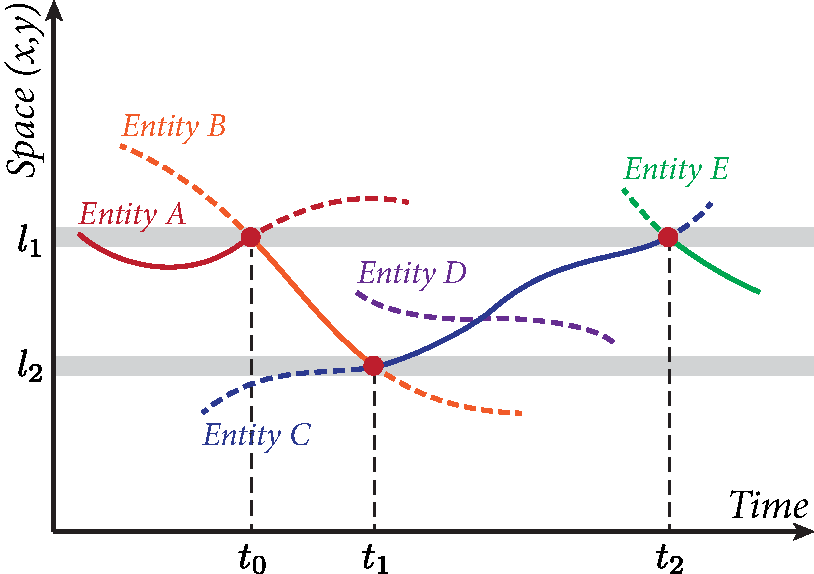
\includegraphics[width=5.3cm]{figures/dtn-indirect-sync-geo.pdf}
    \caption{Indirect synchronous composition between two entities at pre-defined locations.}
    \label{fig:dtn-indirect-sync-geo}
\end{wrapfigure}
Instead of composing the trajectories of the entities anywhere in the geographic area, some strategies only allow the composition at pre-defined locations, as shown in Figure~\ref{fig:dtn-indirect-sync-geo}. In this case, the composition of trajectories can only happen at locations $l_1$ and $l_2$. These strategies exploit the high density of entities and their movement patterns in these areas where the contacts between the entities are more likely to happen (\eg road intersections). These areas have been exploited by context- and location-aware services such as digital graffiti~\cite{carter2004digital} and floating content~\cite{ott2011floating} to anchor content at specific locations. 

In the case of data transfer, the use of these concentrated areas enables a finer control of the routing strategies to limit the number of replications needed when forwarding a data from an area to another. Most of the approaches we review in this section leverage a logical representation of the system with an overlay graph to route the data in the areas on the shortest path. The nodes of the overlay correspond to the areas with high densities of entities and the links represent the movements of the entities between the nodes. 

\paragraph{Determining the locations where to compose the entity trajectories.}
An underlying problem related to this approach is to determine the locations with high densities of entities. In an urban vehicular setting, they correspond to intersections at junctions and traffic lights. In the context of \acrshortpl{vanet}, LOUVRE~\cite{lee2008louvre} and GyTAR~\cite{jerbi2009towards} build an overlay network on top of intersections (``landmarks'' in the case of LOUVRE) where vehicles are connected to each other. When the vehicles come to the intersections, they forward the data over overlay links representing the \acrshort{vanet} multi-hop path between two adjacent intersections. Similarly, Tan~\etal uses the movements of vehicles traveling a transportation network to create a ``vehicular backbone network''~\cite{tan2014vehicular}. The vehicles perform ``wireless switching'' when they are in contact at intersections or on dual-way roads when vehicles travel in opposite directions. Sarafijanovic-Djukic \etal characterize the locations with high entity densities as ``concentration points'' (CP)~\cite{sarafijanovic2006island}. Using real-life traces, the authors defined CPs as areas with at least 5\% of the vehicles per day. In the context of multiple message ferries following different routes and creating a communication medium among static nodes, Zhao \etal propose to pass the data between the ferries at intersecting points of their routes~\cite{zhao2005controlling}. In this case, the ferry routes must be synchronized for the ferries to come in contact regularly. Ker{\"a}nen and Ott propose to transport data between airports using the smartphones of the airline passengers~\cite{keranen2009dtn}. The authors rely on the scheduled flight connections at airports to compose the trajectories of the passengers. 

\paragraph{Maintaining a global view of the network state.}
The entities must have a consistent and up-to-date view of the overlay network to know where and how to forward the data. There are two approaches to knowing this information. The first approach consists in assuming a low-bandwidth control channel to exchange the control messages that have low overhead. This is the case of Tan \etal that uses this control channel to have the latest estimation of the overlay link metrics~\cite{tan2014vehicular}. In the ferry work, Zhao \etal use this control channel to compute the intersecting routes of the ferries in an offline manner~\cite{zhao2005controlling}. The second approach leverages an in-band distributed approach. In~\cite{sarafijanovic2006island}, the entities distribute the information about the overlay using a collaborative graph discovery protocol. While this method does not provide an up-to-date information, it avoids relying on signals from the environment. LOUVRE and GyTAR rely on a peer-to-peer density discovery to populate link state table of the overlay nodes with the density information. However, in the case of a large-scale network such as the airline network proposed by Ker{\"a}nen and Ott, the entities cannot maintain information about all the links in the overlay. The authors argue that epidemic protocols that replicate the data are more suited for this case to forward the data~\cite{keranen2009dtn}.

\paragraph{Forwarding data when in the specific areas.}
With the information about the overlay, the entities can make forwarding decisions in the pre-determined areas to route the data on the shortest path to its destination. With no information on the future trajectories of the entities, \cite{sarafijanovic2006island} propose to replicate the data to multiple entities to increase the chances that at least one will arrive at the next overlay node. Once the data has reached the next entity, an acknowledgment is broadcasted to the previous entity to discard the remaining copies of the data. Tan \etal forward the data to minimize the delivery delay of the data and guarantee the fairness among the flows~\cite{tan2014vehicular}. When two vehicles encounter, they choose the data flow and overlay link that are the least used of those available and the pre-allocated ones. In LOUVRE and GyTAR, the routing protocol uses the well-known Dijkstra algorithm to use the link state tables and forward the data on the overlay links with the highest density of entities~\cite{lee2008louvre,jerbi2009towards}.

Using the spatial distribution of the entities to restrict the composition of the trajectories to areas where entities concentrate allows better control of the forwarding. The logical representation of the network makes the allocation of the data transfers possible and improves the performance of the resulting data transfer compared to the floating case. In the following, we review the strategies that leverage a dedicated infrastructure that temporarily buffer the data to asynchronously compose the trajectories of the entities. As a result, contrary to the synchronous case, they do not have to encounter at the same time and place to pass the data.


\subsection{Asynchronous composition of the trajectories}
\label{sec:indirect-async}

While restricting the compositions of the entity movements to specific locations can improve the forwarding decisions, the movements of the entities between the locations can be unpredictable. To overcome the randomness, other approaches propose to rely on a dedicated infrastructure with intermediate nodes, either mobile or stationary, that temporarily buffer the data carried by the entities before passing it to subsequent entities. In this case, direct contacts between the entities are not required, allowing the data to be passed asynchronously. 

The use of mobile intermediate nodes, such as ferries or robots, allows remote entities to communicate together, even if their trajectories do not intersect. These nodes follow pre-scheduled routes to bridge the trajectories of distant entities. In this case, the composition of the distant entities is asynchronous and floating.

Stationary intermediate nodes, such as offloading spots or throwboxes, enable the communication between two entities whose trajectories do not necessarily intersect at the same time. As a result, these nodes are pre-positioned at specific locations frequently visited by the entities. In this case, the composition of the entities is asynchronous and happens at pre-defined locations.

In the following, we review the strategies that rely on intermediate nodes to support the data transport. In the first part, we review the strategies with mobile nodes and those with stationary nodes in the second part.

\subsubsection{Floating composition}
\label{sec:indirect-async-non-anchored}

% - choose the next node to visit to satisfy the node requirements (dynamic)
% - Communication with the nodes
% - distribution of the global state (distributed vs central)
% - Using multiple message ferries

\begin{wrapfigure}[9]{o}[0.7\marginparwidth]{5.5cm}
    \vspace{-37pt}
    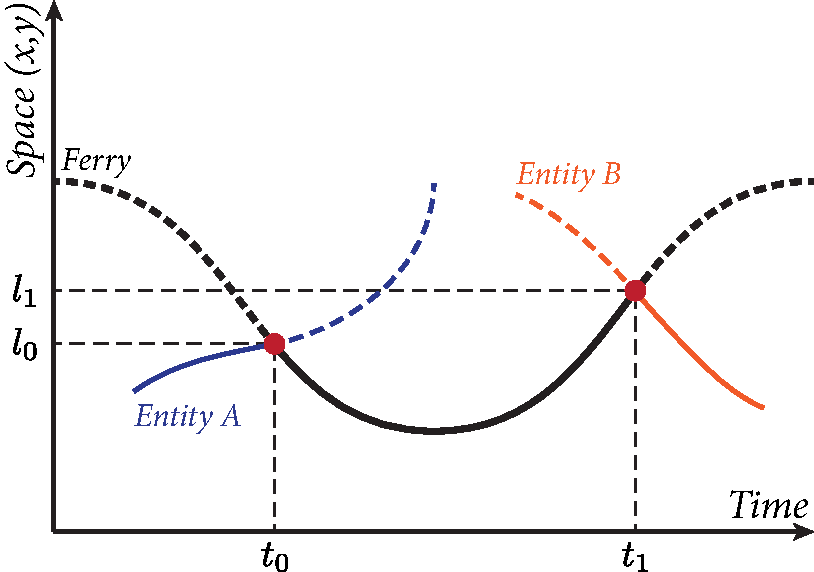
\includegraphics[width=5.3cm]{figures/dtn-indirect-async-nongeo.pdf}
    \caption{Indirect asynchronous floating composition between two entities using a \textit{ferry}.}
    \label{fig:dtn-indirect-async-nongeo}
\end{wrapfigure}
Mobile intermediate nodes, such as ferries or robots enable the composition of the trajectories of remote entities together. As a result, the data is passed asynchronously between the entities. In Figure~\ref{fig:dtn-indirect-async-nongeo}, we represent the asynchronous composition of the trajectories of entities $A$ and $B$ using a ferry that encounters the entities. These intermediate nodes enhance the capacity of the mobile networks by providing more opportunities to compose the movements of the mobile entities. As a result, they provide an on-demand data transport service to serve the requests to transfer data of the entities.

\paragraph{Determining the next entity to visit.}
With mobile entities, the ferries must dynamically determine the next entity to serve to optimize given metrics (\eg bandwidth requirements of the entities). In the \acrfull{fimf} proposed by Zhao \etal, the ferry follows a default route and receives requests from the mobile entities when they want to send data~\cite{zhao2004message}. The ferry then detours from its route to meet the entity and exchange data. The authors focus on the scheduling of the requests received by the ferry and propose a different heuristic to select the next entity to visit. The first heuristic always selects the nearest entity after one has been served, while the second one performs slightly better by using local optimization techniques to solve the \acrshort{tsp} introduced in~\cite{zhao2003message} and recompute the route of the ferry by minimizing the expected data drops. With the \acrfull{nimf} approach, the entities move proactively close to the ferry, which follows a pre-determined route~\cite{zhao2004message}. When an entity detours to meet the ferry, it degrades the performance of its assigned tasks. The authors propose to use a threshold based on the current duration the entities have been working on their tasks for entities to decide whether to come close to the ferry. This decision minimizes the message drop (caused by long delivery delay or buffer overflow) while limiting the detour made by the entities.

\paragraph{Controlling multiple ferries.}
The two approaches we have reviewed so far have considered a single ferry to serve the entities. Having multiple ferries creates additional challenges to scheduling the entities to visit next. This problem can be generally reduced to the dial-a-ride problem~\cite{savelsbergh1985local}. Burns~\etal borrow two multi-objective techniques from robotics for the ferries to optimize a given set of performance metrics~\cite{burns2005mv,burns2008mora,burns2006autonomous}. They consider the subsumption composition, which prioritizes the ordered metrics and optimizes them successively, starting from the higher ones, and each up to a given performance threshold. They also consider the nullspace composition, which outperforms the subsumption composition and orders the metrics such that the optimization of these lower metrics does not affect the performance of the higher metrics. 

\paragraph{Maintaining a global view of the network state.}
To decide which entity to visit next, the ferries must have an up-to-date view of the state of the network. Therefore, communications between the entities and the ferries are important to announce the positions of the ferries and the entities. In both the \acrshort{fimf} and \acrshort{nimf}, the authors propose to use long-range channels to periodically broadcast the position of the ferry and the entities. With multiple ferries, Burns \etal rely on a distributed approach to maintaining an approximate global view of the state of the network at each ferry. This information is exchanged and updated among the ferries when they encounter, which allows them to take online and local decisions to improve the performance of the network given a set of objectives. In both this work and the \acrshort{fimf}, the location of the entities is known to the ferries through either the global state information disseminated in the network or the long-range channel. However, the ferries do not predict the future positions of the entities; they only know their last positions advertised, which can lead to errors when localizing the entities.

\paragraph{Non-controllable dedicated entities.}
While the ferries or robots are dynamically controlled to decide which entity to visit, other approaches propose strategies to use the already-existing movements of dedicated entities that act as ferries to transport the data. In the context of \acrfullpl{mav} used for Search and Rescue missions, Asadpour \etal designed a forwarding algorithm to route the data recorded by hovering \acrshortpl{mav} with onboard cameras to a central ground station~\cite{asadpour2016route,asadpour2013now,asadpour2014micro}. The authors introduce relay \acrshortpl{mav} that physically carry the data between the ground station and the hovering \acrshortpl{mav}. The algorithm relies on an estimate of the future proximity of the \acrshortpl{mav} to the destination, calculated using a linear mobility model of the \acrshortpl{mav} that predicts the future positions in the near future. The algorithm chooses whether to the forward data along the multi-hop shortest path to the destination if there is such a path or if the neighbor is spatially closer to the destination. Otherwise, the algorithm decides to keep the data and carry it on the \acrshortpl{mav} until it encounters the destination or a more suitable \acrshort{mav} (\eg a ferry \acrshort{mav}).

Using mobile intermediate nodes brings more opportunities to compose the trajectories of the entities. They also enable communication between distant entities whose trajectories never intersect. As a result, their use improves the performance of the data transfers, in terms of delivery rate and delay. While these nodes bridge the connectivity between distant entities, they incur additional delays when carrying the data. The delayed deliveries are mainly due to the dynamic schedule of their route. In the following, we review the approaches that use stationary nodes to compose the trajectories of entities.

\clearpage
\subsubsection{Composition at pre-defined locations}
\label{sec:indirect-async-anchored}

\begin{wrapfigure}[11]{o}[0.7\marginparwidth]{5.5cm}
    \vspace{-10pt}
    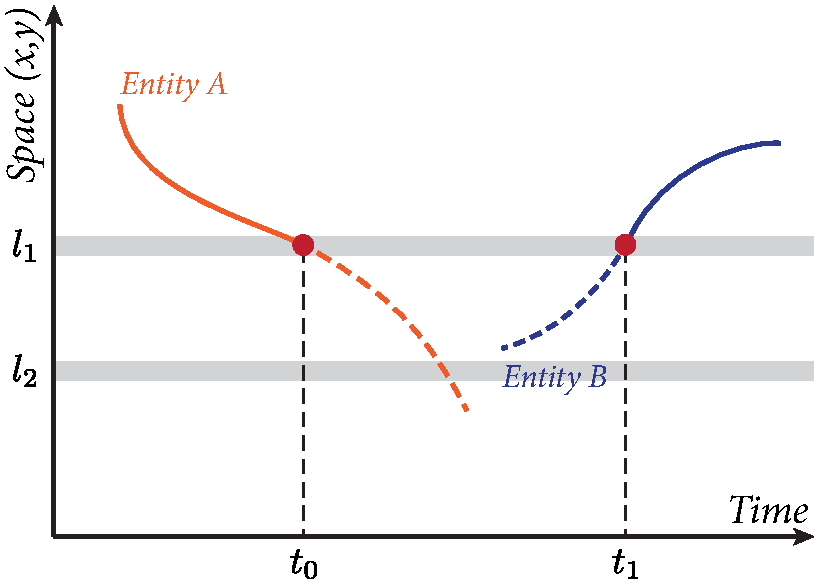
\includegraphics[width=5.3cm]{figures/dtn-indirect-async-geo.pdf}
    \caption{Indirect asynchronous composition between two entities at pre-defined locations using a \textit{stationary nodes}.}
    \label{fig:dtn-indirect-async-geo}
\end{wrapfigure}
In the previous section, we reviewed the approaches that rely on dedicated mobile relays to compose the remote movements of entities and increase the performance of the network. Conversely, other approaches leverage a collection of stationary nodes placed at strategic locations to asynchronously compose the movements of entities with intersecting trajectories. In Figure~\ref{fig:dtn-indirect-async-geo}, we represent the asynchronous composition with stationary nodes at location $l_1$ and $l_2$ that compose the trajectories of entities $A$ and $B$.

% - Placement of the stationary relays to optimize a network metric such as the delivery rate or delay
% - Forwarding of the data at the stationary nodes -> multi-path routing, replication
% - Energy-efficient communications with the entities


\paragraph{Stationary node placement.}
The main problem with this approach is to place the stationary nodes to efficiently compose the trajectories of the entities and optimize performance metrics such as the delivery rate or delay. The stationary nodes must be along the trajectories of the entities to efficiently compose their trajectories. Zhao~\etal introduced \textit{throwboxes} or small inexpensive battery-powered devices equipped with storage and wireless interfaces to enhance the delivery likelihood of mobile ad hoc networks by increasing the contact opportunities~\cite{zhao2006capacity}. The authors use linear programming models and heuristics to deploy the throwboxes based on the different knowledge they consider of the traffic matrix and the future contacts between the entities and the potential candidate locations of the throwboxes. 

In~\cite{chawathe2006inter}, Chawathe proposes to use dead drops\footnote{\url{http://deaddrops.com/}}, an art project that uses USB sticks placed at different locations in cities (\eg on the walls of buildings), to disseminate data using the opportunistic movements of vehicles to transport data from one dead drop to the other. The author proposes a placement of the dead drops using a greedy heuristic of the minimum-weight $k$-set cover problem such that it provides the required connectivity between flows of vehicles traveling different routes of interest at minimum deployment cost. 

\paragraph{Forwarding the data to the entities.}
Once the stationary nodes placed at strategic locations, the next challenge is to forward the data to the entities. With throwboxes, the authors consider different routing strategies~\cite{zhao2006capacity}. With no assumptions on the future contacts among the entities and the throwboxes, the authors propose to use the epidemic protocol between mobile entities and throwboxes. Ibrahim \etal found that allowing any forwarding interactions among the mobile entities and the intermediate nodes reduces the delivery delay of the data at the expense of additional replication~\cite{ibrahim2009analysis}. However, restricting the forwarding to the sole interactions between the mobile entities and the intermediate nodes yields poor performance in terms of delivery delay and the number of copies generated, as the source and destination must come close to an intermediate node to either transmit or receive the data. Banerjee~\etal compare the performance of forwarding strategies with two-hop (no mobile-to-mobile communications), random Epidemic (to limit the number of copies generated by message) and RAPID~\cite{balasubramanian2010replication} in the presence of different kinds of stationary intermediate nodes. The authors found that deploying $x$ base stations (connected together by an infrastructure-based network) allows reducing the average packet delay by a factor of two. The same reduction requires $2x$ mesh nodes (connected together by long range wireless links) and $5x$ relays (acting as throwboxes~\cite{zhao2006capacity}).

The forwarding problem was extensively studied in KioskNet a low-cost alternative that leverages the movements of vehicles between rural kiosks deployed in remote regions with limited Internet connectivity and offers services such as email and land records~\cite{seth2006low,guo2007very,guo2011design}. This creates a mechanical backhaul\index{mechanical backhaul} that transports data between an Internet gateway located in a nearby city and the kiosks. The kiosks serve as routers to forward the data to other kiosks, thus creating an overlay network with the kiosks as intermediate nodes and the movements of the vehicles as links. The authors propose to use different routing strategies, including flooding (does not scale), reverse-path forwarding (fragile in case of failures), and link-state routing, which uses the expected delay between two kiosks as the link weight. 

Following the same architecture as KioskNet, Demmer and Fall propose DTLSR, which modifies the \acrfullpl{lsa} with long lifetimes to take the changes in the connectivity into account~\cite{demmer2007dtlsr}. This avoids considering the node as unreachable if the link to this node is unavailable at the lime of the \acrshort{lsa} is computed, as it is the case in legacy link-state routing. The data is then routed using a shortest-path algorithm (\eg Dijkstra) such that the estimated expected delay is minimized. 

In TrainNet, the authors also formulate the routing problem of carrying data on trains as a fair resource allocation problem~\cite{zarafshan2010trainnet}. Since the trains have limited storage available and only a limited amount of data can be exchanged at stations, the routing problem maximizes the throughput and hard drive utilization, while minimizing the delay and data losses. 

\paragraph{Energy-efficient forwarding.} 
Banerjee \etal propose a framework to enable power savings at throwboxes equipped with solar panels~\cite{banerjee2007energy}. In particular, they focus on improving the neighbor discovery phase, which is the primary source of energy consumption, by using two radio channels to separate the neighbor discovery task from the data transfer task. A long-range channel is in charge of the neighbor discovery task and efficiently listens for contacts (duty-cycle), while a high-bandwidth radio remains asleep. On a contact with the long-range channel, the throwbox determines whether the contact is fruitful by (\textit{i}) predicting the future mobility of the entity and (\textit{ii}) determining whether to accommodate this contact or the future ones based on the current level of energy available and the estimated duration of this contact.

\paragraph{Combination with delivery services.}
The same approach is also used in combination with delivery services, which we introduced in Section~\ref{sec:thrid-party-services}. Wang \etal propose a centralized architecture with either a central server or geo-distributed servers~\cite{wang2004turning}. The servers aggregate the data received from parcels and dispatches it to the final users or route it across the servers, still using the postal services. Adding multiple servers allows the users to send the data to the closest server, thus reducing the costs of sending the data. Cho and Gupta propose a joint use of the Internet with postal services to minimize the cost and latency of the transfer~\cite{cho2010new,cho2011budget}. To this end, they leverage an overlay of the sites connected by both shipping links and Internet links. The overlay links are represented by a capacity, cost and transit time, which vary over time in the case of shipping links (\eg both the cost and transit time vary as a function of the level of service~---~Overnight, Two-day, Ground). The authors reduce their problem to a flow over time problem~\cite{fleischer2007quickest}, which they manage to make tractable with optimizations for large-scale networks. In every case, their system outperforms the single use of the Internet or the shipping method to transfer data. 

\paragraph{Message ferry case.}
Finally, in the case of multiple ferries, the authors propose to use a dedicated infrastructure to pass the data between ferries following different routes~\cite{zhao2005controlling}. The stationary nodes are then placed at the intersections of the ferry routes to compose the trajectories of the ferries. Bin \etal design a ferry route such that a single ferry visits the mobile entities without any online collaboration at determined locations for determined durations with a certain minimum target probability~\cite{bin2006message}. While this approach does not leverage stationary nodes, it results in an asynchronous forwarding restricted to specific locations. To design the route, the algorithm first determines the way-points among a set of candidate points and the corresponding waiting times at these way-points such that the ferry meets the other nodes with a given probability (either while moving or while waiting at a way-point). Second, the algorithms determine the route to follow such that it minimizes the weighted sum of the waiting times and the total distance of selected way-points from the center of the region.

Stationary intermediate nodes have been used in wide-range of applications and give the potential to increase the capacity of the resulting data transfers. Their placement is important to capture the trajectories of the entities to have opportunities to compose them together. This is the approach we have considered with the offloading spots to realize the offloading system we present in this thesis. 


\section{Relevance to the thesis}

In this section, we discuss the relevance of each part of our work with respect to the state-of-the-art we presented in previous sections. 

\paragraph{Vehicular data offloading.} 
In the first part of our work, we rely on offloading spots that act as intermediate relay nodes similar to those used to asynchronously compose entity trajectories at pre-defined locations such as throwboxes~\cite{zhao2006capacity}. In this case, these intermediary nodes create additional contact opportunities and bring the data closer to its destination. They also introduce non-randomness in an environment where entity trajectories are difficult to predict. The authors showed that these nodes are an effective way to compose the entity trajectories and improve the overall throughput and delivery delay.

Our system aims to transfer large amounts of delay-tolerant data, between remote locations. Examples of large data transfers over the Internet range from exchanges of large scientific datasets to distribution of high-resolution movies. Some protocols have been developed to handle bulk data transfers of several  Terabytes per day, such as GridFTP~\cite{allcock2003gridftp} or NetStitcher~\cite{laoutaris2011inter}. The latter takes into account unused bandwidth in inter-data center networks (during low link utilization periods) by using multi-path and store-and-forward scheduling at intermediate nodes for bulk transfers.

While these previous approaches allow transferring bulk data, we propose to \textit{physically offload} data by creating an alternative communication channel consisting of existing vehicle movements. Several works proposed to create such a channel by relying on the movements of entities such as airline passengers~\cite{keranen2009dtn}, trains~\cite{zarafshan2010trainnet}, or even postal services~\cite{wang2004turning,cho2011budget,laoutaris2013delay}. While these approaches are comparable with our work in terms of scale, throughput, and delay, they are difficult to compare under equivalent settings, including the number of entities involved and trips made, as well as their coverage.

\paragraph{Vehicular cloud services.}
In the case of the first extension, we rely on the schedule movements of public buses to distribute user files among repositories. This work is closely related to KioskNet~\cite{seth2006low} and DakNet~\cite{pentland2004daknet}, although they do not provide any performance evaluation and they take place in rural environments with fewer bus routes and trips available. In our system, the bus act as message ferries that connect the repositories together~\cite{zhao2004message}. While they are not controllable, they have the same purpose to connect remote nodes together.

The consumer/producer behavior of the mobile users is similar to the TierStore system, which acts as a Network File System (NFS) for applications with limited bandwidth or challenged network environments~\cite{demmer2008tierstore}. User files are stored in persistent storage repositories that lie at the core of the system (\ie static nodes similar to our repositories). Updates are applied locally at the persistent repository and distributed to other nodes. The system also uses the movements of mobile nodes to distribute updates to and from the nodes using static multicast. On the other hand, Ott and Pitk{\"a}nen proposed to use the mobile nodes to temporarily store content by means of caching~\cite{pitkanen2007redundancy,ott2007dtn} to decrease the latency when retrieving a content. This approach is similar to the one proposed by Haggle, a \textit{Pocket Switching Networking} (PSN) system that enables caching of content at intermediate nodes to also reduce the delivery delay~\cite{scott2006haggle}.

The placement of the repositories in this extension is similar to the placement of throwboxes, where the authors select the optimal locations for throwboxes from a set of candidate locations (\ie centers of square cells dividing the geographical space) to maximize the total data rate, given different knowledge on contact opportunities and traffic load for various routing strategies (\ie single-path, multi-path, and epidemic)~\cite{zhao2006capacity}. However, our placement does not account for the routing strategy, which makes it more related to the one proposed by Chawathe in the context of dead drops to disseminate data~\cite{chawathe2006inter}. In this case, the drop boxes have the same behavior as our repositories and data is disseminated using the (known) movements of vehicles. The placement of dead drops must provide the required connectivity among them at minimum deployment cost and is solved using a heuristic of the minimum-weight $k$-set cover problem fitting the model.

Finally, in the second extension, we leverage pre-defined locations selected such that vehicles encounter for a duration long enough to transfer large amounts of data through vehicle-to-vehicle communications. While these locations are similar to those used for wireless switching by Tan~\etal to create a ``vehicular backbone network''~\cite{tan2014vehicular}, or those used by Sarafijanovic-Djukic \etal to perform data forwarding~\cite{sarafijanovic2006island}, our work studies the capacity of the contacts at specific locations.

\paragraph{Logical view of the vehicle movements.}
Throughout the thesis, we analyze and characterize the vehicles' movements between locations (for the data offloading part and the first extension) or the locations where vehicles are in contact with one another (for the second extension) with a logical view representing the dynamics of the network. Our contribution lies in the fact that we use this view to translate movements into networking quantities and enable the allocation of data transfers. This is the case of the offloading overlay that mitigates the complexity of the road network and represents the flows of vehicles traveling between the offloading spots as resources to allocate. We leverage this logical view in the extensions to deploy the repositories (in the case of the first extension) and the contact hotspots (in the case of the second extension).

\paragraph{Centralized architecture.}
Instead of using a distributed control plane as is the case with most of the related approaches, we leverage a centralized architecture with a controller that has a holistic view of the system to efficiently allocate vehicular resources. In the case of the data offloading, the controller then derives forwarding states from the allocation output and installs them at the offloading spots. With these states installed, the offloading spots are able to decide which buffered data to load on the stopping vehicles. This controller performs additional management tasks, including reliable data transfers, file distribution control (in the case of the first extension), and virtual machine migrations control (in the case of the second extension).
\chapter{Assessing the concept of vehicular data offloading}
\label{cha:feasibility-study}

The objective of this chapter is to assess the concept of data offloading. The main step toward the feasibility of this concept can be stated as follows: 

\begin{displayquote}
\textit{Given the demands to offload data transfers from a conventional data network, how does one select the road network paths and the flows of vehicles matching the data transfer requirements to maximize the revenues of offloading traffic on vehicles over the use of a conventional data network?}
\end{displayquote}

% In this chapter, we address the challenge of efficiently allocating the data transfers to flows of vehicles traveling the roads such that the offloading provider maximizes the revenues of the offloading service. 

We first give an overview of the concepts underlying vehicular data offloading and the operations of the offloading infrastructure. We then present a reference scenario in the context of a network of charging stations for \acrfullpl{ev}. Data is unloaded from or loaded on the \acrshortpl{ev}, without the drivers being aware, while charging their batteries as they usually do. The scenario fits with the recent emerging trends in the \acrshort{ev} market, as car manufacturers and charging stations operators are seeking additional revenues beyond sales from added services offered while \acrshortpl{ev} are being charged~\cite{report2014ChargingTrends}.

We propose an allocation procedure that maximizes the cost-benefit of offloading traffic on the road network compared to transferring the same amount of data on a conventional data network. We formulate this allocation procedure as a \textit{revenue maximization problem}\index{vehicle flow allocation problem!revenue maximization model}. To solve this problem, we use a linear programming model that selects the flows of vehicles that maximize the revenue resulting from offloading data over the road network. 

To solve the revenue maximization problem in a reasonable computational time, we propose a mapping algorithm that creates a logical representation to mitigate the complexity of the road network. In this representation, nodes corresponding to the offloading spots are connected by logical links. A logical link corresponds to the flows of vehicles traveling the road segments connecting two adjacent offloading spots in the road network. We propose a method that derives from the road traffic counts a characterization of the logical links in terms of delay, capacity, and data loss. The offloading overlay mitigates the complexity of the substrate network and makes the allocation of vehicles tractable.

We finally provide numerical results using actual road traffic counts in the road network of France. 

As a summary, the main contributions of this chapter are:

\begin{itemize}

    \item \textbf{Vehicular offloading} (Section~\ref{sec:operations}). We describe the principle of offloading traffic on vehicles. We introduce the concept of \textit{offloading spots}, which refer to storage facilities deployed along the roads. We present a reference scenario involving offloading data on Electric Vehicles while charging their batteries at stations acting as offloading spots.    
    
    \item \textbf{Road map space reduction} (Section~\ref{sec:offloading-overlay}). We design a mapping algorithm to mitigate the complexity of the road network. The output of our algorithm is an \textit{offloading overlay} that gives a comprehensive representation of the underlying resources.
    
    % \item \textbf{Reliable data transfers.} We use replication mechanisms to mitigate the effects of the leakage and satisfy a target leakage tolerance for the offloading demands.
    
    \item \textbf{Revenue maximization problem} (Section~\ref{sec:revenue-maximization-model}). We formulate the \textit{vehicle flow allocation problem} as a novel \acrfull{lp} model. We solve the \acrshort{lp} model so as to determine the logical path that maximizes the expected revenues from offloading data on the road network.
     
	\item \textbf{Real-world assessment} (Section~\ref{sec:revenue-maximization-evaluation}). We evaluate our revenue maximization model on the French road network using \textit{actual road traffic counts}. The results show that the existing mobility of vehicles can accommodate transfers in the order of one Petabyte during a one-week time window.

\end{itemize}

The remainder of the chapter is structured as follows. In Section~\ref{sec:operations}, we present the concept of vehicular offloading by providing an overview of the operations to offload data over the road network. We also present a reference scenario involving electric vehicles and battery charging stations. In Section~\ref{sec:offloading-overlay}, we describe the map reduction procedure that mitigates the complexity of the road network. We introduce the revenue maximization problem in Section~\ref{sec:revenue-maximization-model}. We then formulate the revenue maximization problem as a linear programming model in Section~\ref{sec:revenue-maximization}. In Section~\ref{sec:revenue-maximization-evaluation}, we assess the concept of vehicular offloading by using actual road traffic counts for the French road network. Finally, Section~\ref{sec:revenue-maximization-conclusions} draws the conclusions of this chapter.


\section{Vehicular data offloading}
\label{sec:operations}

\subsection{Offloading infrastructure operations}

In the section, we give a schematic overview of the operations of the infrastructure  in charge of offloading large amounts of delay-tolerant data over the road network. We target data transfers lasting several days that result from provisioning or maintenance activities required for virtual machine migrations or offline backup between data centers. Figure~\ref{fig:offloading-operations} depicts the operations on a fragment of the road network.  

Private vehicles\index{private vehicles} are equipped with one or more removable storage devices such as magnetic disks or other non-volatile solid-state storage devices. We assume that the content of the storage devices is not accessible by the drivers and the data encrypted when piggybacked onto the vehicle. We provide in Section~\ref{sec:discuss} ways to guarantee secure transportation of the data. Vehicles also embed one or more communication network interfaces. 

\begin{figure}[h!]
	\centering
		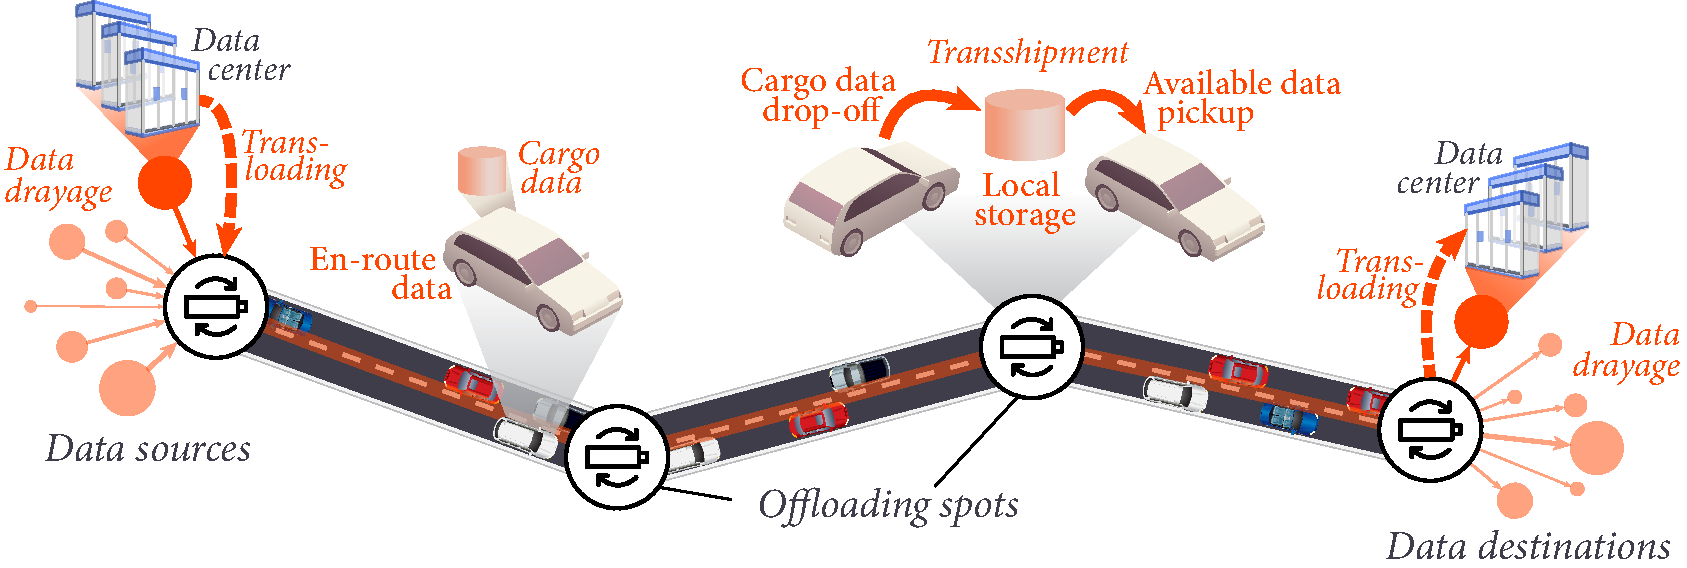
\includegraphics[width=0.95\columnwidth]{figures/taxonomy.pdf}
	\caption{Overview of the operations to offload large amounts of data over the road network.}
	\label{fig:offloading-operations}
\end{figure}

The flow of vehicles so equipped acts as a mechanical backhaul\index{mechanical backhaul} connecting a collection of offloading spots, as depicted in Figure~\ref{fig:offloading-operations}.
%The term \textit{offloading spot}\index{offloading spot|bb} refers to specific locations featured with storage capabilities where vehicles may be parked long and close enough as part of their routines. 
The term \textit{offloading spot} refers to a fixed device offering short- to medium-term data storage, located where vehicles stop for long periods of time as part of their travel route. Examples of such locations include on-street parking spots, parking lots, or gas stations. In the case of electric vehicles, the offloading spots may be located at the battery charging stations such as the ones operated worldwide by ChargePoint\footnote{\url{http://www.chargepoint.com/}}. Offloading spots are equipped with wireless communication interfaces to support short-range radio data exchanges with vehicles while stopped. 

%The offloading service we propose relies on the opportunistic use of private vehicles equipped with storage capacities in combination with a collection of fixed wireless data storage devices referred to as \textit{offloading spots}\index{offloading spot|bb} (as illustrated in Figure~\ref{fig:taxonomy}). Vehicles are equipped with one or more removable storage devices such as hard drives or other non-volatile solid-state drives. Each vehicle carries a \textit{cargo}\index{data cargo|bb} of data in their storage devices. 
%We assume that vehicles also embed a \acrfull{gps} that generates routes and guidance between a geographic location and a destination. The flow of vehicles so equipped acts as a mechanical backhaul\index{mechanical backhaul} connecting a collection of offloading spots. 

%Offloading spots remove the need of relying on the only vehicles making the trip all the way from the source to the destination of a data transfer. 

Offloading spots act as data relay exchange points where data is \textit{transloaded}\index{transloading} from a conventional data network to the closest offloading spot using a \textit{drayage}\index{drayage} system and stored until shipped to its destination by vehicles. Different techniques to implement a data drayage system are presented in Section~\ref{sec:discuss}. We take advantage of the parking time of the vehicle to opportunistically load data on or off their storage devices. 

Vehicles unload their data cargo while they are stopping at an offloading spot if they are heading in a different direction than the destination of the data they carry. The data is stored until transferred to a subsequent empty vehicle heading towards the intended destination. As a result, the data may be transferred on multiple vehicles following different trajectories before reaching its destination. Splitting the data path across different vehicles makes the transfers less vulnerable to hijacking attempts on vehicles. To mitigate the effect of vehicles changing their travel directions or having accidents, offloading spots load the same data on multiple vehicles, either at the first offloading spot or at each intermediate offloading spot.

The data is therefore ``hitchhiked'' hop-by-hop through the network of offloading spots before reaching its final destination. Transfers of offloaded data result from the vehicles' routine journeys interspersed with stops at the offloading spots as part of their line of travel. Offloading spots thus remove the need of relying on the only vehicles making the trip all the way from the source to the destination of a data transfer.

% motivations for the offloading spots

The data offloaded from conventional networks follows the same path as the flow of vehicles traveling the road segments connecting sequences of offloading spots. 
%As depicted in Figure~\ref{fig:offloading-operations}, multiple consecutive offloading spots may be involved if the data needs to be shipped across a large body of country before reaching geographically long distant destinations. 

%To avoid the need of relying on vehicles solely traveling all the way from the source to the destination of the data transfers, offloading spots act as data exchange relay points. Vehicles in contact with an offloading spot unload their cargo if heading to a different direction with the destination of the data transfer. The data is stored until transferred to a subsequent vehicle heading towards the intended destination.
%Given the increasing number of vehicles driven and miles traveled, large chunks of data can be offloaded from an infrastructure network such as the Internet. 
For each offloading demand, the road network path is determined by solving the vehicle flow allocation problem we formulate as a multi-commodity flow allocation model in Section~\ref{sec:revenue-maximization-model}.


% An existing allocation plan may be dynamically modified in case the vehicles change direction unexpectedly or to account for new data transfers as they arrive. The dynamic allocation method we describe is applied to flows of vehicles. Such a flow refers to the group of electric vehicles traveling in the same direction between two adjacent offloading spots. We do not consider the complete journey of each vehicle traveling the underlying road network. The scheduling of the data transfers (\ie the selection of the data to be piggybacked), and the security and privacy issues are out of the scope of this article. In section~\ref{sec:discussion}, we will discuss potential future directions for addressing these issues. 


\subsection{Business model, assumptions, and roles}
\label{sec:business-model}

\begin{figure}[h!]
    \centering
    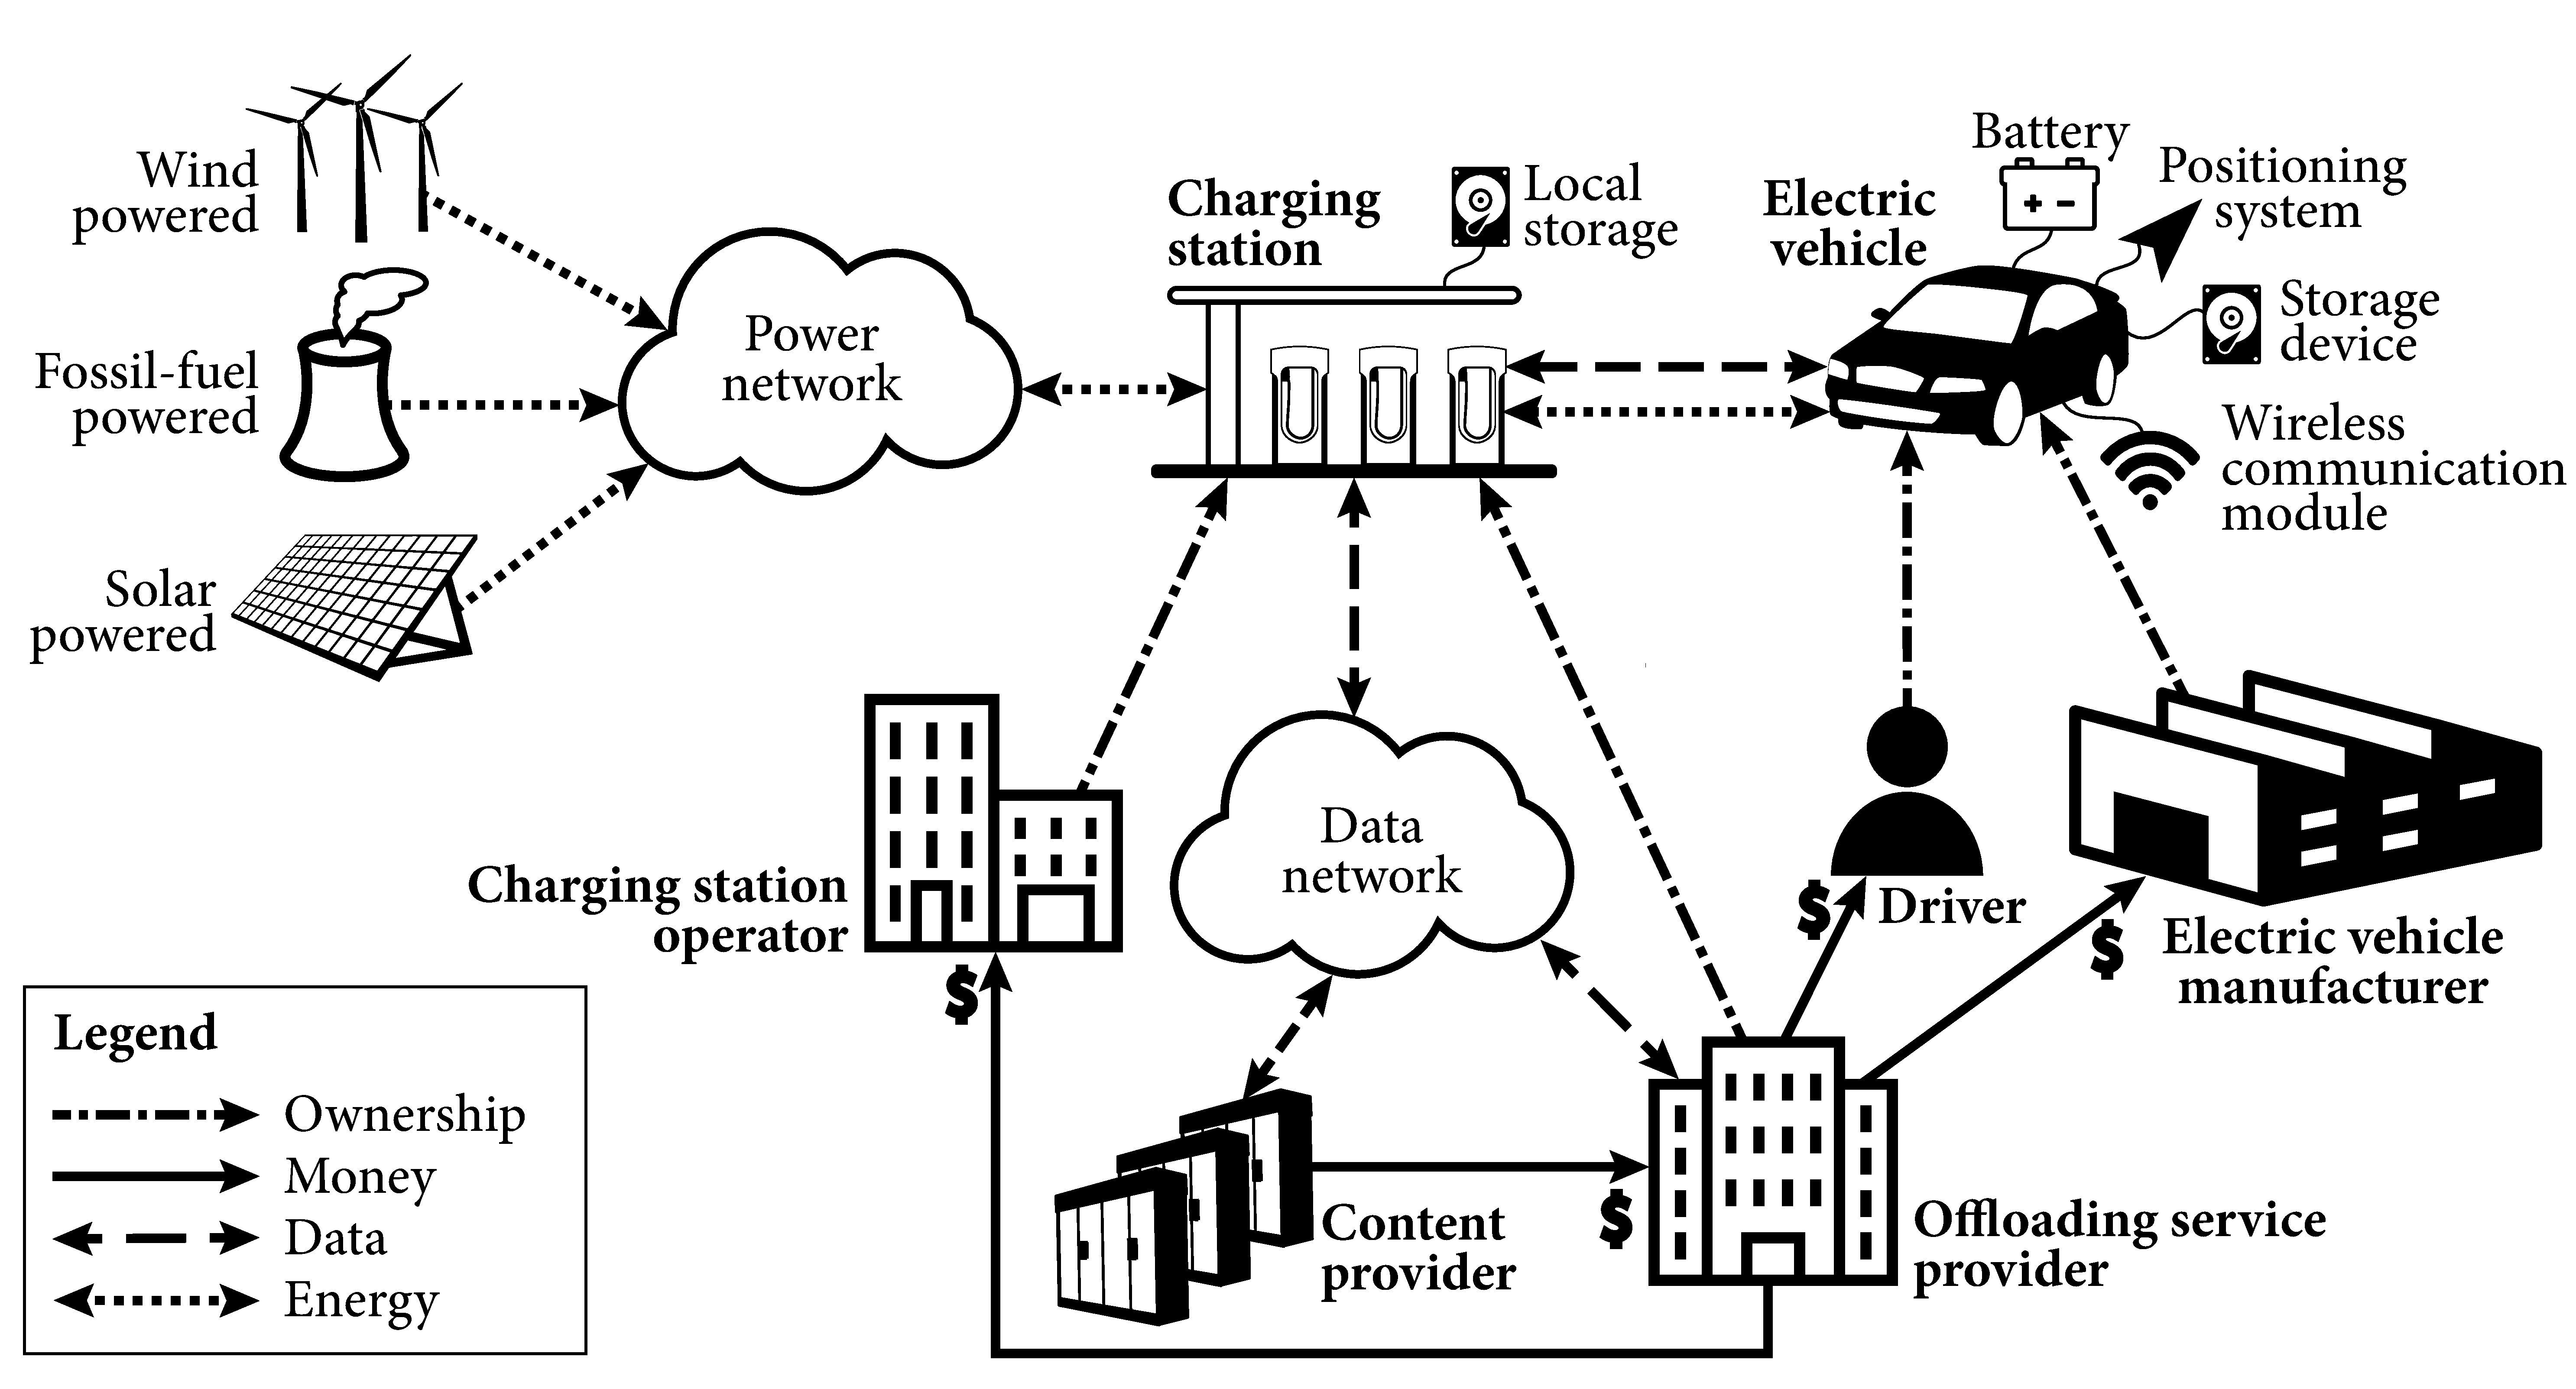
\includegraphics[width=0.9\textwidth]{figures/business-plan.pdf}
    \caption{Business model for the vehicular data offloading concept.}
    \label{fig:business-model}
\end{figure}

In this section, we present the business model we will use throughout this thesis. We represent the different actors involved in Figure~\ref{fig:business-model}, including (\textit{i}) \acrfullpl{ev} and their owners, (\textit{ii}) the offloading service provider (that can be the \acrshort{ev} manufacturers themselves), (\textit{iii}) the charging station operator, and (\textit{iv}) a content provider that operates multiple data centers. 

This model provides support for the modeling and analysis of our proposal in practical settings, including the driving range of \acrshortpl{ev} (\eg 320~km for the Tesla Model S) and the charging time of the batteries (\eg 20~minutes when charging at a Tesla supercharger\footnote{\url{https://www.tesla.com/supercharger}}). 

The electric vehicles are equipped with one or more data storage devices, such as hard drives or other non-volatile solid-state devices. 
%We assume that the content of the storage devices is not accessible by the drivers and the data encrypted when carried onto the vehicle. 
The term ``electric vehicle'' \acrshort{ev} refers to private vehicles propelled by one or more electric motors powered by a rechargeable battery. %Commercial vehicles may be part of a fleet owned or leased by a business or a governmental agency. 
%We assume that vehicles also embed one or more communication network interfaces. 
The charging stations act as \textit{offloading spots} where the data is seamlessly loaded on or unloaded from the onboard storage of the vehicles using short-range radio while they charge their battery. 

The offloading service provider, if different from the \acrshort{ev} manufacturers, proposes a ``get paid to drive'' program to the car owners. The service provider installs the storage devices and the vehicle owners receive a monthly fee or a discount on the cost of charging their vehicle in exchange for driving their normal routine. The discount rate is negotiated with the charging station operator (\eg ChargePoint who operates a worldwide network of \acrshort{ev} charging stations offering cloud-network services\footnote{\url{http://www.chargepoint.com/}}) and is calculated based on the driving pattern including coverage and mileage. If the \acrshort{ev} manufacturers take on the role of service provider, vehicles are equipped as standard with onboard storage and the service is provided without involving nor compensating the vehicles' drivers. The service provider charges the content provider for the amount of data to offload on the road network and shares the revenues with the charging station operator. 
%The offloading spots may also comprise battery swap stations where vehicles' memory implemented as removable devices are replaced with ready-to-ship devices so that vehicles can continue their travels without waiting for the data to be transferred.  

%Offloading spots act as intermediate data exchange relay points. Offloading spots enable the transshipment of data chunks as they can be dropped off for future pick-up by subsequent passing vehicles. The offloading spots transfer a data chunk on a charging vehicle using short-range radios. Every time a vehicle stops by an offloading spot, its destination is matched against the destination of the data chunk 

The offloading spots feature storage capabilities where data is transloaded from the conventional data network and temporarily stored 
%as \textit{data cargo}\index{data cargo} 
until transferred to a charging vehicle. 
%The content provider uses a border dray transfer system if the data originates from a distant repository, typically a wide-area data network such as the Internet connecting the content provider to the edge offloading spots. 
The service provider monitors the status of the offloading spots, which includes the amount of available storage and the destination of the data cargo in transshipment. To improve the forwarding decisions, the service provider also queries the stopping vehicles' positioning system to determine their current geographic destination. The historical locations are stored in a geographic location database managed by the service provider to help the offloading spots predict the remaining itinerary of the passing vehicles.  In Section~\ref{sec:discuss}, we present a list of probabilistic tools for inferring the remaining route of a vehicle knowing its navigation history and discuss the concerns regarding the drivers' and passengers' privacy.

%The service provider receives the demands to offload data transfers from the content provider. Each demand specifies the delay and bandwidth requirements for the corresponding data transfer. The service provider keeps track of the status of the offloading spots which include statistics about the charging vehicles. The offloading spot operator also reports information about the data cargo locally unloaded for later pickup. The service provider, which collects the information from the offloading spots, has an up-to-date view of the offloading infrastructure.

Upon receiving a demand to offload a data transfer from a content provider, the service provider computes the road network paths that can accommodate the data transfer requirements and how much data to allocate to each flow of vehicles. The road network path consists of a sequence of offloading spots, each configured with the list of actions to perform on each vehicle traveling in the direction of the next-hop offloading spot. Each action defines the behavior that the offloading spot operator needs to perform with the data belonging to the offloaded transfer. The corresponding data can either be already stored at the offloading spot or carried by the charging vehicle. Common actions include loading data cargo on or off the vehicles while charging their battery. The service provider defines these actions based on the information the offloading spot operator reports on the flows of vehicles passing through the offloading spots. For each vehicle stopping by an offloading spot, the offloading spot operator matches the destination of the vehicle against the data transfers currently offloaded on the road network and performs the actions as dictated by the service provider. 

\section{Road map reduction}
\label{sec:offloading-overlay}

Recall that our objective in this chapter is to assess the vehicular offloading concept by comparing the cost of using the offloading infrastructure including the offloading spots compared to the cost charged by Internet providers for transferring the same amount of data. We need to determine the routes followed by the vehicles carrying the data and offering the same performance as the one resulting of transferring the same amount of data on the Internet. 

To determine those routes, we present a revenue maximization model in Section~\ref{sec:revenue-maximization-model}. Before solving this model, we need to cope with the scale of the road network. The high degree of complexity of the road network's topology and the large number of vehicular trips make the revenue maximization problem computationally intractable.

In this section, we present a mapping algorithm that reduces the complexity of the road network. The output of our algorithm is an offloading overlay\index{offloading overlay|bb}, which refers to a logical representation that captures the characteristics of the road network. We provide a performance evaluation that measures the reduction factor resulting from the mapping algorithm by comparing the complexity of the offloading overlay over the actual road network.


\subsection{Road network}
\label{sec:road-network-characterization}

We represent the road network\index{road network|bb} by a directed graph $G^R=(N^R,\,L^R)$, where $N^R$ and $L^R$ denote the set of physical nodes and links, respectively. The set of nodes $N^R=N^J\cup N^S$ consists of two subsets: the set of road junctions ($N^J$) and the set of charging stations ($N^S$). A road junction refers to a location where vehicles can change their direction of travel. A link in the road network corresponds to a road segment connecting two adjacent junctions or a junction and a charging station. We consider the road segments and the traffic flowing in both directions homogeneous as they share the same profile in terms of capacity. For a road segment $(a,\,b)\in L^{R}$, let $v_{ab}$ be its nominal volume of vehicles (vehicles per unit of time), $c_{ab}$ be its capacity (vehicles per unit of time), and $t_{ab}(v_{ab})$ be its corresponding travel time that depends on the nominal volume of vehicles. 

We use publicly available datasets to characterize the road network. These datasets feature traffic volumes on the road segments, expressed in terms of \acrfull{aadt}\index{AADT}. \Acrshort{aadt} is the total volume of traffic traveling on a road segment in both directions for one year, divided by the number of days in the year. As a result, the capacity $c_{ab}$ of a road segment $(a,\,b)\in L^{R}$ are fixed to the \acrshort{aadt} value of the dataset for this road segment.


\subsection{Offloading overlay}
\label{sec:offloading-overlay-characterization}

\begin{wrapfigure}[15]{o}[0.7\marginparwidth]{7.5cm}
    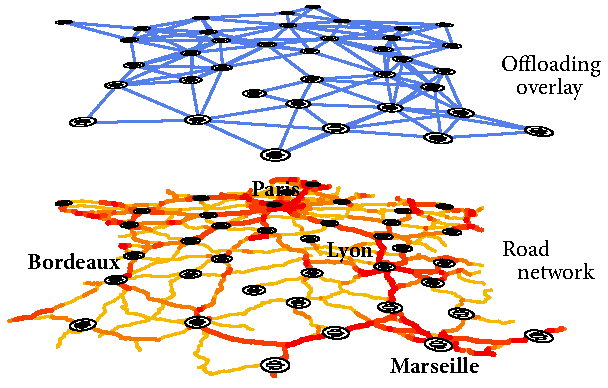
\includegraphics[width=7cm]{figures/France-overlay-1.pdf}
    \caption{The offloading overlay resulting from the deployment plan of battery charging stations acting as offloading spots for the French road network (the width and darkness of the road segments denote the vehicle density).}
    \label{fig:France-overlay}
\end{wrapfigure}
The offloading overlay\index{offloading overlay|bb} provides a logical representation\index{logical representation} of the road network. More specifically, the overlay mitigates the combinatorial explosion when enumerating the simple road paths in the road network, which becomes quickly intractable when the length of the paths increases. By providing a logical representation\index{logical representation} of the vehicle flows on the road paths connecting the offloading spots, the offloading overlay reduces the number of paths to enumerate. 
%and makes the data transfer allocation problem tractable.

We represent the offloading overlay by a directed graph $G^O=(N^O,\,L^O)$, where $N^{O}$ and $L^{O}$ denote the set of logical nodes and links, respectively. A logical node of $N^{O}$ is an offloading spot. A logical link of $L^{O}$ represents the road path (\ie a sequence of road segments) connecting two adjacent offloading spots in the road network. Note that, multiple road paths may connect two adjacent offloading spots, in which case, the logical link aggregates these paths. In Figure~\ref{fig:France-overlay}, we show an example of realization of an offloading overlay on top of the French road network. 

In the following Section~\ref{sec:characterization-offloading-overlay}, we characterize a logical link $(i,\,j)\in L^{O}$ with network quantities, that is by the weighted travel time $t(i,\,j)$, aggregated capacity $c(i,\,j)$ and data leakage $l(i,\,j)$. The data leakage refers to the loss rate on logical link $(i,\,j)\in L^{O}$ and accounts for the proportion of vehicles that fail to deliver the data to the next offloading spot $j$ because of errors in the prediction of the direction of the vehicle or accidents. We assume that offloading spots are not constrained by the amount of transfers they can serve and have the adequate storage capacity so that the overall service is stable. 


\subsection{Characterization of the offloading overlay} 
\label{sec:characterization-offloading-overlay}

In this section, we characterize the logical links of the offloading overlay into network quantities. The network quantities we consider in the following are relevant to solve the revenue maximization problem.

\paragraph{Travel time $t(i,\,j)$.} 
 The travel time $t{ab}$ of $(a,\,b)$ is given by the \acrfull{bpr} function defined as~\cite{BPR64}:

\begin{equation}
  \label{eq:BPR}
  t_{ab}(v_{ab})=t_{ab}(0)\left[1+\alpha\left(\frac{v_{ab}}{c_{ab}}\right)^{\beta}\right]\Comma
\end{equation}

\noindent where $\alpha$ and $\beta$ are \acrshort{bpr} parameters that depend on the road profile ($\alpha = 0.15$ minutes and $\beta = 4.0$ are typically used)~\cite{HCM00}.

We can deduce from Equation~\ref{eq:BPR} the travel time of physical path $p$, denoted $t_{p}$, which is the sum of all travel times of the road segments that compose the path (we do not consider any turning delays at junctions):

\begin{equation}
  \label{eq:path-delay}
  t_{p} = \sum_{(a,\,b)\in p} t_{ab}(v_{ab}).
\end{equation}

From Equation~\ref{eq:path-delay}, we deduce an expression of the average travel time\index{logical link!average travel time} $t(i,\,j)$ experienced on the $r$ physical paths between nodes $i$ and $j$, weighted by the road traffic flow $v_{p}$ on each path $p$:

\begin{equation}
  \label{eq:ovelray-link-delay}
  t(i,\,j) = \frac{\sum_{p\in S_{ij}} t_{p}\,v_{p}}{\sum_{p\in S_{ij}}v_{p}}\Comma
\end{equation}

\noindent where $S_{ij}$ is the set of all simple physical paths between $i$ and $j$ (\ie with no cycles in the path).

\paragraph{Capacity $c(i,\,j)$.}
The capacity\index{logical link!capacity} $c(i,\,j)$ of the overlay link $(i,\,j)\in L^{O}$ depends on the sum of the traffic flows $v_{p}$ of the simple paths between offloading spots $i$ and $j$ (\ie the number of vehicles per unit of time going from $i$ to $j$ on path $p$). The capacity $c(i,\,j)$ of the overlay link also depends on the market penetration ratio\index{market penetration ratio|bb} $\mathcal{M}$ of the vehicles participating in the data offloading and the storage size\index{storage size} $\mathcal{S}$ on each vehicle. We assume that all vehicles are equipped with a storage device of the same size $\mathcal{S}$.

\begin{equation}
  c(i,\,j) = \mathcal{M} \mathcal{S} \sum_{p\in \mathcal{P}^{ij}} v_{p}.
\end{equation}

In the performance evaluation presented in Section~\ref{sec:revenue-maximization-evaluation}, we derive the value of $v_{p}$ for each path $p$ from the French road network dataset. This dataset provides the real traffic counts in terms of \acrshortpl{aadt} for the road segments composing each path $p$.

\paragraph{Leakage $l(i,\,j)$.}
The leakage\index{logical link!leakage} $l(i,\,j)$ (comprised between 0 and 1) of logical link $(i,\,j)\in L^{O}$ represents the proportion of data that is lost between offloading spots $i$ and $j$. The leakage increases as more vehicles carrying data prematurely exit the road (\eg the vehicles may exit the highway before reaching the offloading spot or an accident may have occurred). The leakage depends on characteristics that are inherent to the physical paths mapped in the offloading overlay. Additionally, the leakage accounts for the errors inherent to the prediction of the direction of the vehicles when loading data at an offloading spot.

\section{Revenue maximization model}
\label{sec:revenue-maximization-model}

In this section, our objective is to assess the concept of vehicular offloading. The main step towards the feasibility of this concept can be stated as follows: Given a demand to offload a data transfer from a conventional data network, how does one select the road network paths and the flows of vehicles to match the demand requirements. 

We introduce the revenue maximization model\index{vehicle flow allocation problem!revenue maximization model|bb} that maximizes the cost-benefit of offloading traffic on the road network instead of using a conventional data network. We assume that the data is replicated in multiple copies each transferred over different vehicles to the next offloading spots. We devise two replication models resulting in two separate formulations of the revenue maximization models. 

\subsection{Offloading demands}
\label{sec:offloading-demands-feasibility}

An offloading demand\index{offloading demand} $d_{st}$ represents a request to offload a data transfer from a source offloading spot $s\in N^{O}$ to a target offloading spot $t\in N^{O}$. The demand is characterized by the amount of data $\beta_{st}$ and the deadline $\tau_{st}$ before which the transfer should be completed. Recall from Section~\ref{sec:offloading-overlay-characterization}, that we need to account for the vehicles that fail to reach the next offloading spot on time. Thus, each offloading demand is also characterized by a leakage tolerance $l_{st}$. We denote by $\mathcal{D}=\{d_{st}\}$ the matrix of the offloading demands indexed by the pairs of source and destination offloading spots $(s,\,t)$ of the corresponding data transfers. The leakage tolerance $0 < l_{st} \leq 1$ refers to the data loss ratio tolerated during the transfer on the road network, provided that the data is replicated at the source according to redundancy techniques (\eg Reed-Solomon or \acrshort{raid})~\cite{chen1994raid}, combined to the use of error correcting codes~\cite{macwilliams1977theory}. The leakage tolerance is consistent with the data encoding mechanism. Note that, $\beta_{st}$, the total amount of data to be transferred between $s$ and $t$, includes the redundant data introduced by the redundancy techniques. 

In the vehicle flow allocation model, $p$ denotes a logical simple path\index{logical path|bb} (\ie without any cycles) defined as the ordered list of offloading spots connected by logical links. $\mathcal{P}_{st}$ denotes the set of all logical simple paths from $s$ to $t$. We characterize the logical paths by the travel time $t(p)$ and the data flow (throughput) $f(p)$ allocated on logical path $p\in\mathcal{P}_{st}$ for a given offloading demand $d_{st}$ resulting from the vehicle flow allocation problem. The logical path travel time corresponds to the average time it takes to transfer one data cargo from one extremity of the path to the other. 


\subsection{Replication models}
\label{sec:replication-models}

We assume that the sequence and the properties of the links comprising the path followed by a data transfer remain unchanged for the time of the observation. We consider that offloading spots undertake two different behaviors when incoming vehicles unload their data cargo:

\begin{itemize}

	\item \textbf{Local replication (\textit{rep}).}\index{reliability!replication model!local replication} This model assumes that all offloading spots replicate data on multiple outgoing vehicles. For a given offloading demand $d_{st}$ and for each adjacent offloading spot $j$, offloading spot $i$ replicates data $\rho_{st}(i,\,j)$ times vehicles traveling on logical link $(i,\,j)\in L^{O}$ (\ie the same data is loaded onto $\rho_{st}(i,\,j)$ vehicles heading to $j$). This logical link is characterized by the leakage $l(i,\,j)$. The amount of replication needed is calculated such that it satisfies the leakage tolerance $l_{st}$ of the offloading demand. 

	\item \textbf{Source replication (\textit{nrep}).}\index{reliability!replication model!source replication} The second model assumes that none of the offloading spots replicate data on the outgoing vehicles, except at the source offloading spot. It takes into account the combination of the leakage on the logical links that compose logical path $p$, denoted by $l_{p}(i,\,j)$ for the resulting leakage at logical link $(i,\,j)$. Here, we assume the source can characterize the entire paths to be allocated using traffic forecasting techniques before the transfer happens~\cite{de2011modelling,sheffi1985urban}. For path $p$ and demand $d_{st}$, the source offloading spot $s$ replicates the data $\rho_{st}(p)$ times such that it satisfies the leakage tolerance $l_{st}$ of the offloading demand. 

\end{itemize}

\subsection{Cost model} 

We aim to measure the cost-benefit\index{cost model|bb} of offloading data over a solution relying on conventional data networks when delivering the same amount of data. We consider a offloading demand $d_{st}$ characterized by the amount of data to transfer $\beta_{st}$ and the transfer duration $\tau_{st}$ we target. Our model describes the cost-benefit of a data transfer, defined as the difference between the price charged by an \acrfull{isp} for transferring $\beta_{st}$ within $\tau_{st}$, and the operational costs induced by transferring data with the offloading infrastructure. In the following, we define the Internet-based price and the operational costs.

\begin{itemize}
	
	\item \textbf{Internet-based cost.}\index{cost model!Internet-based cost} $\gamma_{st}$ is the unit cost to send a bit of data from $s$ to $t$ over the legacy Internet (\eg a leased line between $s$ and $t$). As an example, $\gamma_{st}$ may vary in function of the distance between $s$ and $t$. Without loss of generality, we assume that $\gamma_{st}$ is linear with the volume of data transferred. $\gamma_{st}$ may also be seen as the savings one can achieve by using our offloading infrastructure instead of an Internet-based solution.
	
	\item \textbf{Operational costs.}\index{cost model!operational costs} $\alpha_{i}$ is the operational cost needed for the maintenance of the storage facility at offloading spot $i$, as well as the financial compensations given to the drivers of the vehicles involved in the data offloading. We assume $\alpha_{i}$ is also linear with the volume of data exchanged at offloading spot $i$. The value of $\alpha_{i}$ depends on the replication model we consider. $\alpha^{\text{rep}}_{i}$ corresponds to the local replication model and $\alpha^{\text{nrep}}_{i}$ corresponds to the source replication model. The local replication model will require the data to be stored for longer periods of time. Each copy is held until it can be transferred to a vehicle matching the destination of the data. Hence, the need for extra storage facilities will induce higher operational costs for the local replication model $\alpha^{\text{rep}}_{i}$, compared to the source one $\alpha^{\text{nrep}}_{i}$.
	
\end{itemize}

Note that we do not explicitly consider the \acrfull{capex} to deploy the infrastructure required to offload data over the road network. The \acrshort{capex} includes the storage facilities at the offloading spots and the storage devices installed on the vehicles. Instead, we consider the infrastructure already deployed and exploited by the offloading spot operator (\eg the charging station operator\index{charging station operator}). Hence, the \acrshort{capex} costs are amortized and thus accounted for in the operational costs we consider.

In the following, we present our revenue maximization model\index{vehicle flow allocation problem!revenue maximization model} as a \acrlong{lp} model derived from a \acrlong{mcf} allocation model\index{multi-commodity flow allocation}. The model maximizes the overall cost-benefit of offloading the entire set of demands $\mathcal{D}$ between each pair of (source, destination). Our cost model constraints the objective by both the delay tolerance $\tau_{st}$ and the capacity $c(i,\,j)$ of the logical links. We summarize in Table~\ref{tab:main-variables-feas} the variables we use in our model.

\begin{table}[!t]
    \caption{Table of notations for the revenue maximization problem.}
    % increase table row spacing, adjust to taste
    \renewcommand{\arraystretch}{1.1}
    \centering
    % Some packages, such as MDW tools, offer better commands for making tables
    % than the plain LaTeX2e tabular which is used here.
    {\footnotesize
    \begin{tabular}{c|l}
        \textbf{Variable} & \textbf{Meaning}\tabularnewline
        \hline 
        $d_{st}$ & Offloading demands between source $s$ and destination $t$\tabularnewline
        $\tau_{st}$ & Delay tolerance of demand $d_{st}$\tabularnewline
        $l_{st}$ & Leakage tolerance of demand $d_{st}$\tabularnewline
        $\beta_{st}$ & Amount of data transferred for demand $d_{st}$\tabularnewline
        $\mathcal{P}_{st}$ & Set of simple paths between $s$ and $t$ on the offloading overlay\tabularnewline
        $\mathcal{S}$ & Storage capacity of the vehicles (cargo size)\tabularnewline
        $\mathcal{M}$ & Market penetration ratio\tabularnewline
        $\gamma_{st}$ & Internet-based cost for demand $d_{st}$\tabularnewline
        $\alpha_{i}$ & Operational cost at offloading spot $i$\tabularnewline
        $\delta_{i}$ & Waiting time at offloading spot $i$ (to load data)\tabularnewline
        $f(p)$ & Flow allocated on logical path $p$\tabularnewline
        $t(p)$ & Travel time of logical path $p$\tabularnewline
        $\rho_{st}(p)$ & Replication factor for demand $d_{st}$ on path $p$\tabularnewline
        $\rho_{st}(i,\,j)$ & Replication factor for demand $d_{st}$ on link $(i,\,j)\in L^{O}$\tabularnewline
        $t(i,\, j)$ & Weighted travel time of logical link $(i,\, j)\in L^{O}$\tabularnewline
        $c(i,\, j)$ & Capacity of logical link $(i,\, j)\in L^{O}$\tabularnewline
        $l(i,\, j)$ & Leakage of logical link $(i,\, j)\in L^{O}$\tabularnewline
        $l_{p}(i,\, j)$ & Combined leakage of logical path $p$ at link $(i,\, j)\in L^{O}$\tabularnewline
    \end{tabular}}
    \label{tab:main-variables-feas}
\end{table}

In the following, we formulate the revenue maximization problem using the offloading overlay with a linear programming model that aims at maximizing the cost-benefit of offloading data over the road network. We consider a snapshot of the system, \ie a state of a system characterized by given parameters valid for the duration of the data transfers (offloading demands, road traffic flows, travel time and  leakage on logical links).

\section{Data offloading revenue maximization}
\label{sec:revenue-maximization}

In Section~\ref{sec:revenue-maximization-model}, we described the revenue maximization model we consider that maximizes the cost-benefit of offloading data transfers on the road network. Here, we present the two revenue maximization models which differ depending on the data replication models used for the data transfers.

The travel time\index{logical path!travel time} $t(p)$ experienced on logical path $p\in \mathcal{P}$ is the sum of the travel times $t(i,\,j)$ on the logical links of $p$ and the waiting time $\delta_{i}$ at each intermediate offloading spot on the path:
\begin{equation}
    t(p) = \sum_{(i,\,j)\in p} \big(t(i,\,j) + \delta_{i}\big).
    \label{eq:feas-logical-path-travel-time}
\end{equation}

For the same offloading demand, the transfer of an amount of data $\beta_{st}$ is constrained by the delay tolerance $\tau_{st}$ and does not depend on the data replication model. Hence, the delay constraint is the same for both models. The delay to transfer $\beta_{st}$ between $s$ and $t$ is the sum of the duration to transfer this quantity over all logical paths between $s$ and $t$ and the average travel time experienced on these paths, weighted by the flow on each path. The delay constraint is expressed as:

\begin{equation}
    \frac{\sum_{p\in \mathcal{P}_{st}}f(p)t(p)}{\sum_{p\in \mathcal{P}_{st}}f(p)} + \frac{\beta_{st}}{\sum_{p\in \mathcal{P}_{st}}f(p)} \leq \tau_{st}.
    \label{eq:delay-constraint-0}
\end{equation}

Equation~\ref{eq:delay-constraint-0} is not a linear expression, which can lead to some difficulties to solve the linear optimization problem. But it can be rewritten as the following linear expression:

\begin{equation}
    \sum_{p\in \mathcal{P}_{st}}f(p)\left(\tau_{st} - t(p)\right) \geq \beta_{st}.
    \label{eq:delay-constraint}
\end{equation}


\subsection{The ``local replication'' model}
\label{sec:rep-model}

Recall that, in this model\index{reliability!replication model!local replication}, every offloading spots store and replicate data. Consider a given offloading demand $d_{st}$ with leakage tolerance $l_{st}$ and $p\in\mathcal{P}_{st}$ a path between $s$ and $t$. If $\rho_{st}(i,\,j)f(p)$ data is transmitted on overlay link $(i,\,j)\in p$, $f(p)$ data is received at destination offloading spot $j$. Here, the replication factor $\rho_{st}(i,\,j)$ is calculated by each offloading spot $i$ that sends data to remote offloading spot $j$ on logical link $(i,\,j)\in L^{O}$ as a function of $l_{st}$ and $l(i,\,j)$ as follows:

\begin{equation}
    l(i,\,j)^{\rho_{st}(i,\,j)}\leq l_{st} \implies
    \rho_{st}(i,\,j) \geq \frac{\log(l_{st})}{\log(l(i,\,j))}\cdot
\end{equation}

The flow on logical link $(i,\,j)\in L^{O}$ is expressed as the sum of all flows sent by offloading spot $i$ to offloading spot $j$ on logical link $(i,\,j)$ for offloading demand $d_{st}$. The flow is constrained by the capacity of the logical link $c(i,\,j)$:

\begin{equation}
    \sum_{s,\,t\in \mathcal{D}\vphantom{\mathcal{P}_{st}}} \sum_{\substack{p\in \mathcal{P}_{st}\\p\ni (i,\,j)}} \rho_{st}(i,\,j)\, f(p) \leq c(i,\,j).
\end{equation}

Recall that, the cost-benefit is expressed as the difference between the cost of an Internet-based service (using the cost factor $\gamma^{st}$) and the operational costs of the offloading infrastructure (costs $\alpha_{i}^{\text{rep}}$ at each offloading spot $i$). Our objective is to maximize the cost-benefit of offloading data, expressed as follows:

\begin{equation}
    \label{eq:total-revenue-obj}
    \sum_{s,\,t\in \mathcal{D}\vphantom{N^{O}}}\beta_{st}\gamma_{st} - \sum_{i\in N^{O}\vphantom{N^{O}}}\alpha_{i}^{\text{rep}} \sum_{p\ni i\vphantom{N^{O}}}f(p).
\end{equation}

One can note that the contribution to the value of Equation~\ref{eq:total-revenue-obj} of each $f(p)$ is negative. Besides, the only lower bonding constraint on $f(p)$ is Equation~\ref{eq:delay-constraint}, which can be interpreted as a requirement on the total flow between each pair $(s,\,t)$. Therefore, maximizing the cost-benefit tends to minimize $\sum f(p)$, and Equation~\ref{eq:delay-constraint} is tight at optimality. It is thus possible to replace $\beta_{st}$ in Equation~\ref{eq:total-revenue-obj} as follows.

% We note that if Equation~\ref{eq:total-revenue-obj} is optimal (i.e., maximize), then Equation~\ref{eq:delay-constraint} becomes an equality since the quantities $\beta_{st}$ are constrained only in the latter equation and $\gamma^{st} > 0$. Now, if we consider an equality instead of an inequality for the delay constraint Equation~\ref{eq:delay-constraint}, when replacing $\beta_{st}$ with its expression, the maximal gross margin objective can be rewritten as:

\begin{equation}
    \sum_{s,\,t\in \mathcal{D}\vphantom{\mathcal{P}_{st}}} \sum_{p\in \mathcal{P}_{st}\vphantom{\mathcal{P}_{st}}} f(p) {\left[\gamma_{st}\big(\tau_{st} - t(p)\big) - \alpha^{\text{rep}}(p)\right]},
    \label{eq:total-revenue-obj-1}
\end{equation}

\noindent where $\alpha^{\text{rep}}(p) = \sum_{i\in p}\alpha_{i}^{\text{rep}}$.

In Equation~\ref{eq:total-revenue-obj-1}, if $\gamma^{st}\big(\tau_{st} - t(p)\big) - \alpha^{\text{rep}}(p)$ is negative, then $f(p)$ is null (objective function decreases otherwise). Hence, from Equation~\ref{eq:total-revenue-obj-1}, we have:

\begin{equation}
    t(p) + \frac{\alpha^{\text{rep}}(p)}{\gamma_{st}} \geq \tau_{st} \implies f(p) = 0.
    \label{eq:cutoff-rep}
\end{equation}

\noindent Since Equation~\ref{eq:cutoff-rep} is a weight on the logical paths (resulting from the weights of the logical links) that depends only on the offloading overlay, we can narrow the search space of the paths that do not satisfy Equation~\ref{eq:cutoff-rep}. Finally, the formulation can be reduced to the cost-benefit maximization objective subject to the capacity constraint on each logical link $(i,\,j)$:

\begin{flalign*}
    & \text{Maximize } \sum_{s,\,t\in \mathcal{D}\vphantom{\mathcal{P}_{st}}}\sum_{p\in \mathcal{P}_{st}\vphantom{\mathcal{P}_{st}}} f(p)\psi_{st}^{\text{rep}}(p), &
    \shortintertext{subject to}
    & \sum_{s,\,t\in \mathcal{D}\vphantom{\mathcal{P}_{st}}} \sum_{\substack{p\in \mathcal{P}_{st}\\p\ni (i,\,j)}} \rho_{st}(i,\,j) f(p) \leq c(i,\,j) \qquad \forall (i,\,j)\in L^{O},
\end{flalign*}

\noindent where $\psi_{st}^{\text{rep}}(p)=\gamma_{st}\big(\tau_{st}-t(p)\big)-\alpha^{\text{rep}}(p)$ can be considered as a weight on logical path $p\in\mathcal{P}_{st}$.

\subsection{The ``source replication'' model}
\label{sec:nrep-model}

In this model\index{reliability!replication model!source replication}, data is replicated at the source offloading spot to satisfy the leakage tolerance $l_{st}$ of the offloading demand $d_{st}$. We assume again that the source can characterize all logical simple paths between the source $s$ and the destination $t$ so it can compute the resulting path leakage $l_{p}(i,\,j)$ for every logical link $(i,\,j)$ in logical path $p\in\mathcal{P}_{st}$. 

We denote by $l_{p}(i,\,j)$ the multiplied leakage experienced at logical link $(i,\,j)\in L^{O}$ on logical path $p$. If $p=(i_{0},\,\dotsc,\,i_{n}),\,i_{k}\in N^{O}$ is a logical simple path between $i_{0}$ and $i_{n}$, then for all $0 \leq k < n$, the leakage $l_{p}(i_{k},\,i_{k+1})$ at logical link $(i_{k},\,i_{k+1})\in L^{O}$ is expressed as:

\begin{equation}
    l_{p}\left(i_{k},\, i_{k+1}\right)=1-\prod_{j=1}^{k}\big(1 - l\left(i_{j-1},\, i_{j}\right)\big),
\end{equation}

\noindent where $0 \leq k < n$. Since the source $s$ knows the attributes of the logical path $p$, it may deduce the replication factor $\rho_{st}(p)$ introduced in Section~\ref{sec:replication-models}. For offloading demand $d_{st}$ allocated on logical path $p=(s,\,i_{1},\,\dotsc,\,i_{n-1},\,t)\in\mathcal{P}_{st}$, the replication factor $\rho_{st}(p)$ is calculated by the source $s$ as follows:

\begin{equation}
    l_{p}(i_{n-1},\,t)^{\rho_{st}(p)} \leq l_{st} \implies
    \rho_{st}(p) \geq \frac{\log(l_{st})}{\log(l_{p}(i_{n-1},\,t))}\cdot
\end{equation}

For each logical link $(i,\,j)\in L^{O}$, the capacity constraint limits to the logical link capacity $c(i,\,j)$ the amount of assigned flows $f(p)$ for each path $p$ that go through the logical link $(i,\,j)$ with the proportion of leftover flow at the logical link $1 - l_{p}(i,\,j)$ and replication factor $\rho_{st}(p)$ for offloading demand $d_{st}$:

\begin{equation}
    \sum_{s,\,t\in \mathcal{D}\vphantom{\mathcal{P}_{st}}} \sum_{\substack{p\in \mathcal{P}_{st}\\p\ni (i,\,j)}} \rho_{st}(p) \big(1 - l_{p}(i,\,j)\big) f(p) \leq c(i,\,j).
\end{equation}

As in the local replication model, the cost-benefit is expressed as the difference of the cost of an Internet-based service (with the cost factor $\gamma_{st}$) and the operational cost of the offloading infrastructure $\alpha^{\text{nrep}} \ll \alpha^{\text{rep}}$. In this model, we also aim at maximizing the cost-benefit of offloading data:

\begin{equation}
    \sum_{s,\,t\in \mathcal{D} \vphantom{\mathcal{P}_{st}}}\left[\beta_{st}\gamma_{st} - \smashoperator{\sum_{i\in N^{O} \vphantom{\mathcal{P}_{st}}}} \alpha_{i}^{\text{nrep}} \smashoperator[l]{\sum_{j\in N(i) \vphantom{\mathcal{P}_{st}}}} \smashoperator[r]{\sum_{\substack{p\in \mathcal{P}_{st}\\p\ni (i,\,j)}}} \rho_{st}(p) \big(1 {-} l_{p}(i,\,j)\big) f(p)\right].
\label{eq:maximization-obj-0}
\end{equation}

If Equation~\ref{eq:delay-constraint} is optimal, then it turns into an equality since it is the only equation that constrains $\beta_{st}$, given that $\gamma^{st} > 0$. Therefore, we can rewrite Equation~\ref{eq:maximization-obj-0} as follows:

\begin{equation}
    \sum_{s,\,t\in \mathcal{D} \vphantom{\mathcal{P}_{st}}} \smashoperator[r]{\sum_{p\in\mathcal{P}_{st}\vphantom{\mathcal{P}_{st}}}} f(p) \negmedspace \left[\gamma_{st}\big(\tau_{st} {-} t(p)\big) {-} \negmedspace \smashoperator{\sum_{\substack{p\in \mathcal{P}_{st}\\p\ni (i,\,j)}}}\alpha_{i}^{\text{nrep}} \! \rho_{st}(p) \big(1 {-} l_{p}(i,\,j)\big)\right].
\label{eq:maximization-obj}
\end{equation}

In Equation~\ref{eq:maximization-obj}, we note that if the factor of $f(p)$ is negative, then, since $f(p)\geq 0$, the objective function decreases, making it non-optimal. Thus, if the factor of $f(p)$ is negative, the flows $f(p)$ must be null. From the former Equation~\ref{eq:maximization-obj}, we have:

\begin{equation}
    t(p) + \frac{\rho_{st}(p)}{\gamma_{st}} \smashoperator{\sum_{\substack{p\in \mathcal{P}_{st}\\p\ni (i,\,j)}}} \alpha_{i}^{\text{nrep}} \big(1 - \mathcal{L}_{p}(i,\,j)\big) \geq \tau_{st} \implies f(p) = 0.
    \label{eq:cutoff-nrep}
\end{equation}

\noindent Similar to Equation~\ref{eq:cutoff-rep}, Equation~\ref{eq:cutoff-nrep} is a weight on the logical paths (although, not resulting from the weights of the logical links) that only depend on the offloading overlay; we can narrow the search space of the paths that do not satisfy Equation~\ref{eq:cutoff-nrep}.

Finally, the formulation can be reduced to the total revenue maximization objective subject to the capacity constraint on each logical link $(i,\,j)\in L^{O}$:

\begin{flalign*}
    &\text{Maximize }\sum_{s,\,t\in \mathcal{D}\vphantom{\mathcal{P}_{st}}}\sum_{p\in \mathcal{P}_{st}\vphantom{\mathcal{P}_{st}}} f(p)\psi_{st}^{\text{nrep}}(p), &
    \shortintertext{subject to}
    & \sum_{s,\,t\in \mathcal{D}\vphantom{\mathcal{P}_{st}}} \smashoperator[r]{\sum_{\substack{p\in \mathcal{P}_{st}\\p\ni (i,\,j)}}} \rho_{st}(p) \big(1 - l_{p}(i,\,j)\big) f(p) \leq c(i,\,j) \qquad \forall (i,\,j)\in L^{O}, & 
    \shortintertext{where}
    &\psi_{st}^{\text{nrep}}(p)=\gamma_{st}\big(\tau_{st}-t(p)\big)- \smashoperator{\sum_{\substack{p\in \mathcal{P}_{st}\\p\ni (i,\,j)}}} \alpha^{\text{rep}}(p)\rho_{st}(p)\big(1 - \mathcal{L}_{p}(i,\,j)\big). &
\end{flalign*}

The amount of data transferred $\beta_{st}$ within the delay tolerance $\tau_{st}$ imposed by offloading demand $d_{st}$ is deduced from Equation~\ref{eq:delay-constraint}:

\begin{equation}
    \beta_{st} = \sum_{p\in\mathcal{P}_{st}} f(p)\big(\tau_{st} - t(p)\big).
    \label{eq:total-transfer}
\end{equation}

We can finally obtain from Equation~\ref{eq:total-transfer} the average throughput of offloading demand $d_{st}$ by dividing the amount of data $\beta_{st}$ by the duration of the transfer $\tau_{st}$.

\clearpage
\section{Performance evaluation on the French road network}
\label{sec:revenue-maximization-evaluation}

In this section, we evaluate the performance of the revenue maximization problem by comparing the throughput resulting from the cost-benefit maximization under varying parameters, including the Internet-based cost, delay tolerance, leakage tolerance, and logical link leakage.

\subsection{Dataset of French road traffic}

\begin{wrapfigure}[17]{o}[0.7\marginparwidth]{7cm}
    \vspace{-20pt}
    \centering
    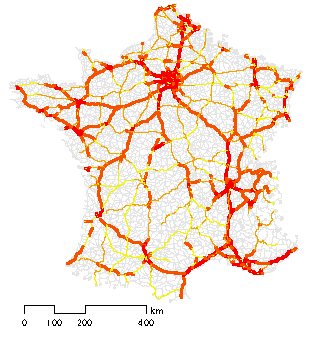
\includegraphics[width=6.8cm]{figures/france-dataset.pdf}
    \caption{Dataset showing the \acrfull{aadt} of the major roads of France in 2011. The road segments have a darker shade when \acrshort{aadt} is higher.}
    \label{fig:france-dataset}
\end{wrapfigure}
We use a dataset\index{French road network} collected in 2011 featuring the \acrfull{aadt}\index{AADT} of the major roads in France covering a combined distance of 20,000~km\footnote{\acrshort{entd}~---~Census of the road traffic on the French roads in 2011 (in French): \url{http://tinyurl.com/otfbewv}}.  The traffic volumes are collected using strategically located automatic traffic recorders. The different thickness and shades of red of the road segments depicted in Figure~\ref{fig:france-dataset} reflect the traffic counts given by the \acrshortpl{aadt}. The graph consists of 3,310 edges covering over 20,000~km of roads. 

\subsection{Planning of the network of charging stations}
\label{sec:charging-station-network}

We consider a network of charging stations similar to the one Tesla\index{Tesla} is currently rolling out in Europe and North America\footnote{\url{https://www.Teslamotors.com/supercharger}}. This network of stations helps electric vehicles face the problem of limited autonomy and achieve long distance travels. Recall that the offloading process will take place in these stations in a transparent manner to the driver. Since there was no such a network in France at the beginning of this thesis, we plan a simple yet realistic network of stations that covers the major roads of France. To plan such a network of stations, we consider a facility-allocation problem\index{facility-allocation problem} that minimizes the number of facilities to allocate, a problem we adapted from the maximal covering location problem~\cite{church1974maximal}. The problem takes demand points and candidate locations as inputs:
\begin{itemize}

	\item The demand points are the 9,555 cities of France with a population greater than 1,000.
   
	\item The candidate locations are the 1,024 Total gas stations, a French oil company.\footnote{\url{http://www.total.fr/mes-deplacements/outils-en-mobilite/export-gps-stations.html} (in French)}

\end{itemize}

The facility-allocation algorithm selects the stations such that a maximum demand points are allocated to the charging stations within a range of 150~km, while minimizing the number of chosen stations. We assume that vehicle ownership is uniform throughout the territory~---~we can then weight the cities by their population. The chosen stations are allocated at most 150~km away from each other. This is enough for a vehicle with an autonomy of 300~km to reach the next closest station or return to the same station without depleting its battery. Finally, we assume that the stations have a capacity that suits the demand such it avoids any waiting time at the stations. The waiting time is then restricted to the service time, which corresponds to the duration of the battery charge.

The resulting allocation outputs 38 stations scattered on the French road network, as shown in Figure~\ref{fig:France-location-allocation}. We note that the stations are mainly allocated near major cities, as the demand from urban areas is higher than from rural areas.

\begin{figure}[ht]
    \centering
    \begin{subfigure}[t]{0.47\columnwidth}
            \centering
            % \raisebox{.2\textwidth}{
            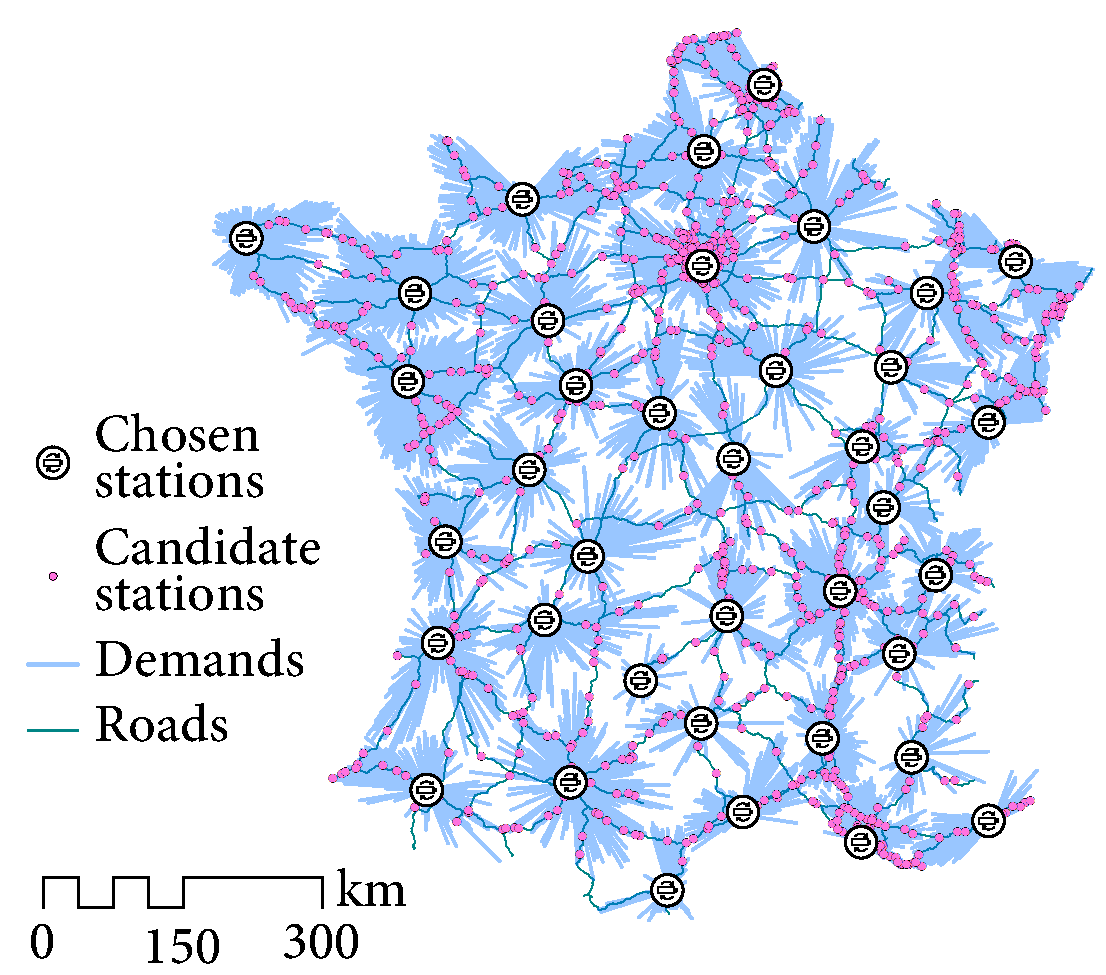
\includegraphics[width=0.98\textwidth]{figures/France-allocation-charging-stations.pdf}
            % }
            \caption{Charging station allocation over the French road network. The big dots are the chosen stations, the small dots are the candidate stations, and the lines represent the allocated demands to the chosen stations.}
            \label{fig:France-location-allocation}
    \end{subfigure}%
    \quad %add desired spacing between images, e. g. ~, \quad, \qquad etc.
      %(or a blank line to force the subfigure onto a new line)
    \begin{subfigure}[t]{0.5\columnwidth}
            \centering
            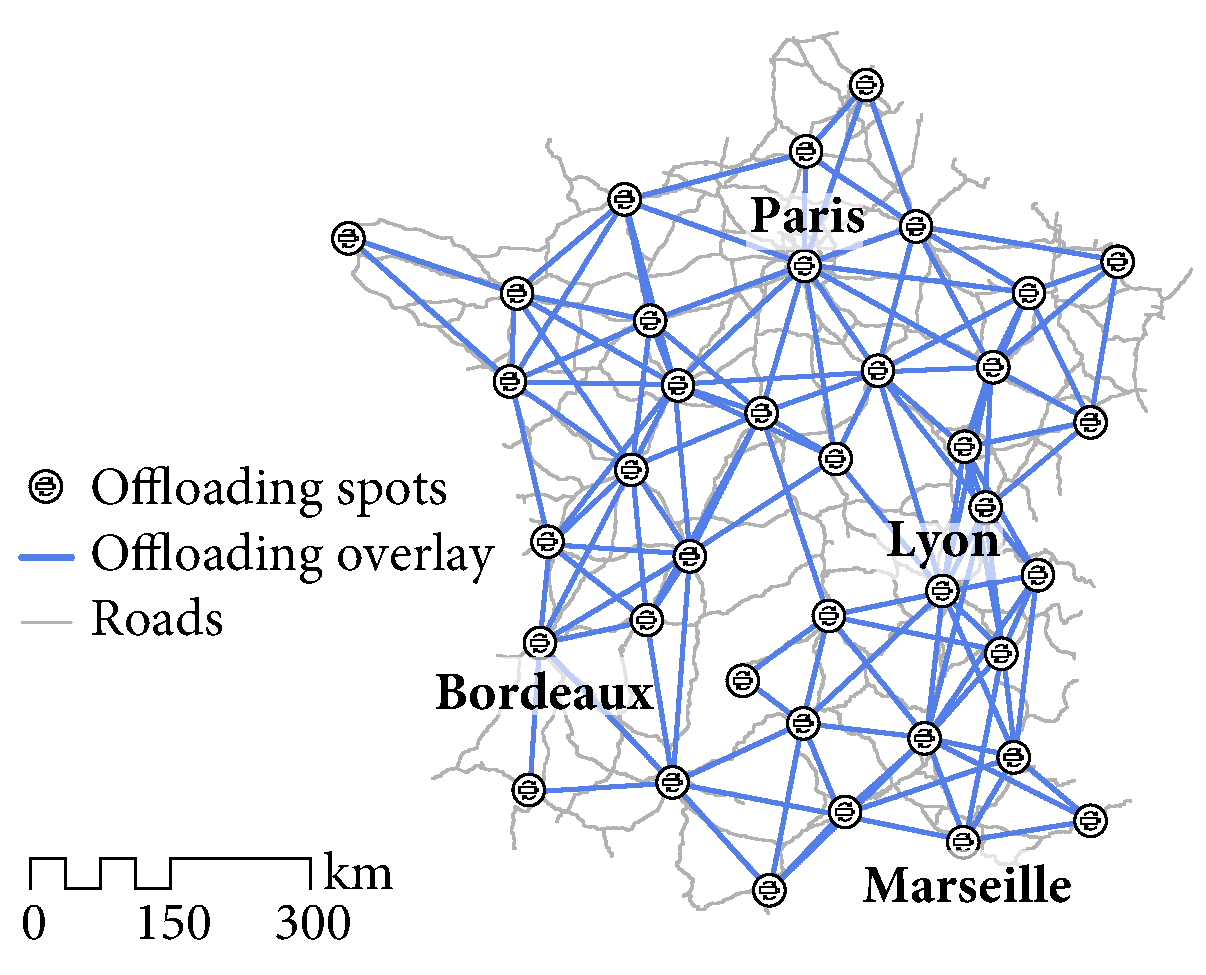
\includegraphics[width=\textwidth]{figures/France-overlay-wo-capacity.pdf}
            \caption{Resulting offloading overlay built on to of the road network of France. The offloading spots are those represented in Figure~\ref{fig:France-location-allocation}.}
            % (deduced from the AADT values)
            \label{fig:France-overlay-wo-capacity}
    \end{subfigure}
    \caption{Facility-allocation result and offloading overlay. The big dots are the chosen stations.}
\end{figure}

In the following, we first provide this characterization with conservative assumptions on the road traffic between the offloading spots. Second, we run the revenue maximization problem we introduced in Section~\ref{sec:revenue-maximization-model} on the offloading overlay for three large-scale data transfers. 


\subsection{Characterization of the offloading overlay}
\label{sec:eval-offloading-overlay}

With the network of stations planned in the previous section, we derive the offloading overlay as defined in Section~\ref{sec:offloading-overlay-characterization}. To compute the resulting overlay depicted in Figure~\ref{fig:France-overlay}, we use the All-or-Nothing traffic assignment strategy that assigns all the road traffic between a source and a destination to the shortest path, here defined as the path with the lowest travel time~\cite{de2011modelling,sheffi1985urban} (refer to the Appendix~\ref{cha:traffic-forecasting-techniques}). Note that, this strategy is conservative in terms of road traffic assigned to the road path. The road traffic flow on this path is set to the minimum \acrshort{aadt} of the road segments composing the path. Then, we use the results of the most recent French travel household survey made in 2008 (\acrfull{entd}) to weight the road traffic on the path by the proportion of trips that travel the length of the path. This survey distinguishes two kinds of travels: local travels are shorter than 80~km from home, while long-distance travels are greater than 80~km from home.

According to the same survey, long-distance travels account for about, in average, 2.8\% of the total amount of travels recorded. This kind of travel is of interest when offloading data since it corresponds to the case where vehicles are likely to stop at more than two offloading spots to charge their depleted batteries while on a trip. We assume the proportion of long-distance travels is uniform  on all the road segments. We consider a market penetration ratio\index{market penetration ratio} $\mathcal{M}$ of 20\% and a storage size $\mathcal{S}$ of one Terabyte assumed to be the same for each electric vehicle. Recall that market penetration ratio corresponds to the proportion of vehicles equipped with storage capabilities and able to participate in the data offloading.

Since the \acrshort{aadt} is measured in both directions of a road segment, we divide the measured values by two. To compute the throughput of the logical link, we multiply the resulting flow by $\mathcal{S}$. We use the \acrshort{bpr} function (Equation~\ref{eq:BPR}) to calculate the travel time on each road segment with: $\alpha = 0.15$ minutes, $\beta = 4.0$, the practical capacity of each road segment given by the dataset, and the \acrshort{aadt} of the road segment for the assigned volume. We use then Equation~\ref{eq:ovelray-link-delay} to deduce the travel time of the logical links using the shortest physical road paths.


\subsection{Benefits of the offloading overlay}
\label{sec:complexity-offloading-overlay}


\begin{wrapfigure}[14]{o}[0.7\marginparwidth]{7.5cm}
    \vspace{-15pt}
    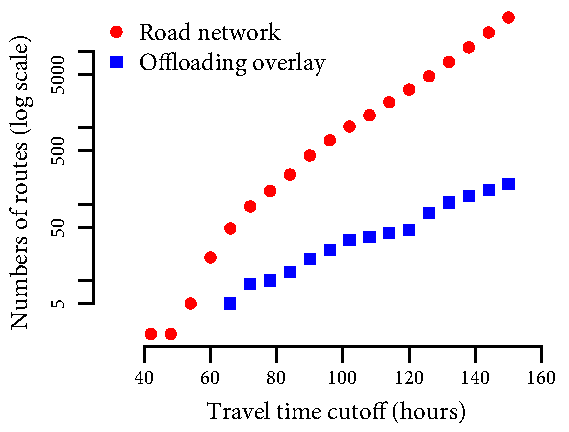
\includegraphics[width=7.2cm]{results/pathcount.pdf}
    \caption{Total number of simple paths in the road network and in the offloading overlay as a function of the travel time cutoff ($y$-axis is in a logarithmic scale).}
    \label{fig:pathcount}
\end{wrapfigure}
For this evaluation, we enumerate all the possible simple paths in both the offloading overlay and the road network. This evaluation shows the benefits of the offloading overlay in mitigating the complexity of the road network. 

We plotted the total number of simple paths bounded by a travel time cutoff in both the road network and the offloading overlay. The plot is represented in Figure~\ref{fig:pathcount} and shows the number of all simple paths as a function of the travel time cutoff of the enumerated paths. In both cases, the number of simple paths grows exponentially with the travel time cutoff. The number of simple paths is much larger on the road network compared to those enumerated in the offloading overlay. Also, the difference in the number of paths grows exponentially. This exponential growth is the main complexity factor to consider when solving the vehicle flow allocation problem.


\subsection{Revenue maximization of offloading data}
\label{sec:res-revenue-max-model}

We interface the offloading overlay we created with \acrshort{cplex} using the linear optimization models we presented in Section~\ref{sec:revenue-maximization-model}. We consider a scenario with the following three different offloading demands (distances are Euclidean) we represent in Figure~\ref{fig:france-demand-allocation-feasibility}:

\begin{itemize}

	\item Offloading demand $d_A$: from Paris to Lyon (384~km).

	\item Offloading demand $d_B$: from Paris to Bordeaux (492~km).

	\item Offloading demand $d_C$: from Paris to Marseille (646~km). 

\end{itemize}

\begin{wrapfigure}[14]{o}[0.7\marginparwidth]{8cm}
    \vspace{-5pt}
    \centering
    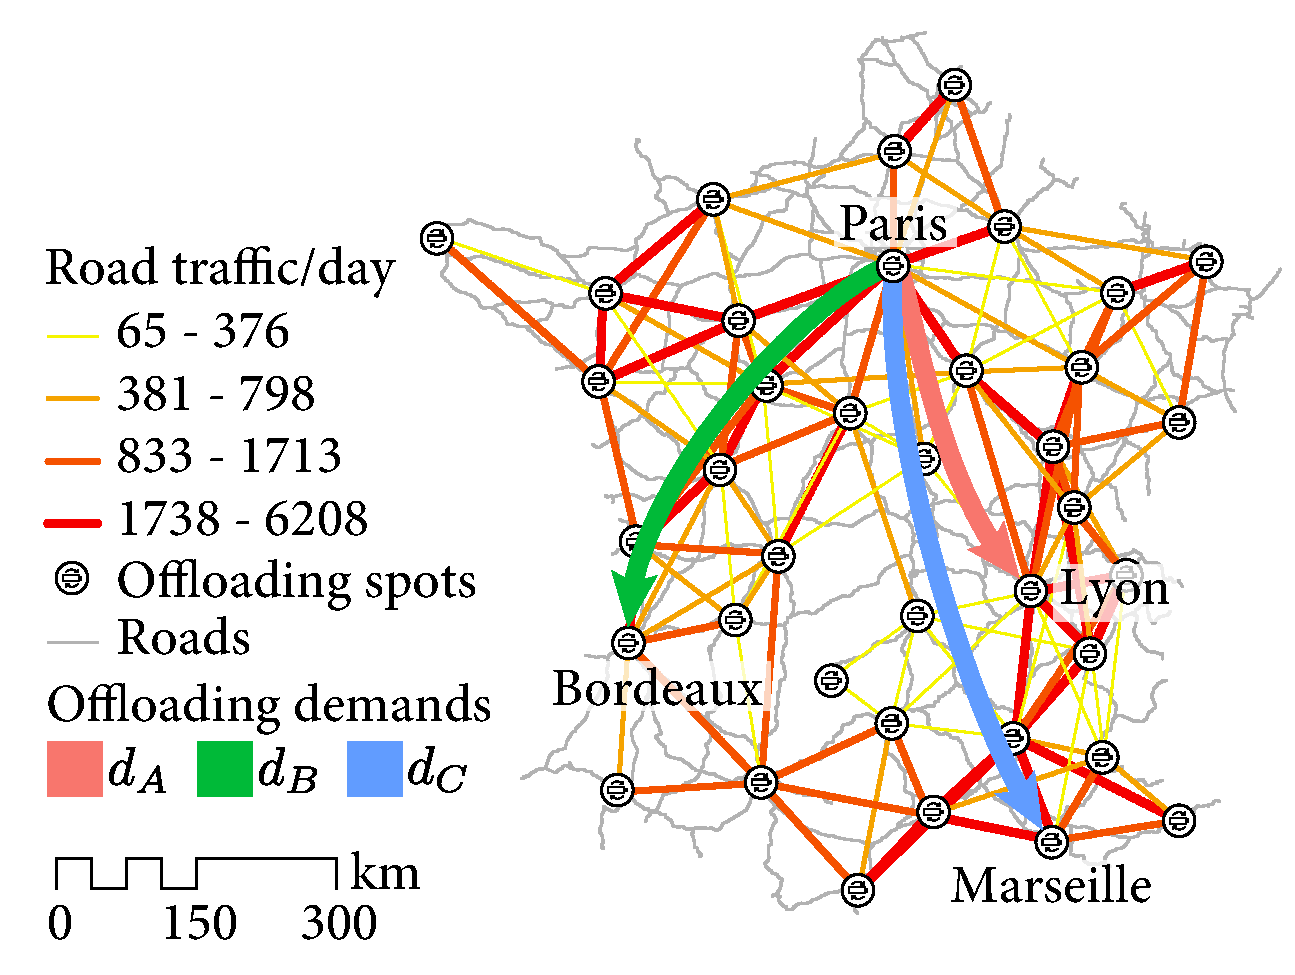
\includegraphics[width=7.8cm]{figures/France-overlay-feasibility.pdf}
    \caption{Schematic representation of the demands $d_A$, $d_B$, and $d_C$.}
    \label{fig:france-demand-allocation-feasibility}
\end{wrapfigure}
It is important to note that demands $d_A$ and $d_C$ will compete for the flows since they share some common subpaths, as we will see in Figure~\ref{fig:allocation-subpaths-offloading-overlay}. This leads to fairness issues, as competing demands will be favored over other demands with the cost-benefit maximization objective, depending on how well they perform. In the following, we discuss how to ensure fairness among the competing flows.

We use a breadth-first search algorithm to generate all the simple logical paths on the offloading overlay for each offloading demand. The cutoffs of the simple paths are given by Equations~\ref{eq:cutoff-rep} and~\ref{eq:cutoff-nrep} for the local replication \textit{rep} and source replication \textit{nrep} models, respectively. However, the generation of the simple logical paths between a source and a destination is exponential, as seen in Figure~\ref{fig:pathcount} of the previous chapter. To solve this issue, we reduce our search space by applying a default cutoff of 12 hours on the travel time of the simple logical paths we generate for our experiments. A 12-hour cutoff is sufficient for each generated path to cover all end-to-end trips within France and small enough to avoid unnecessary path computation.

\begin{wrapfigure}[14]{o}[0.7\marginparwidth]{7.5cm}
    \vspace{-15pt}
    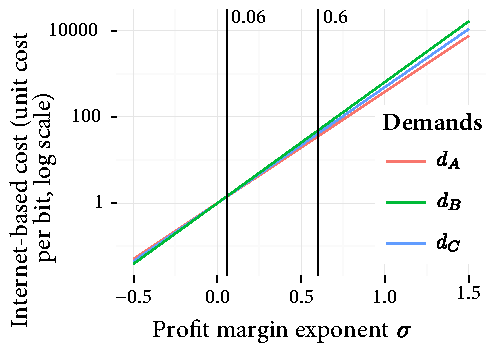
\includegraphics[width=7.2cm]{results/ton-demand-price-km.pdf}
    \caption{Internet-based cost (expressed as the unit cost per bit transferred) as a function of the profit margin exponent for each demand $d_A$, $d_B$, and $d_C$.}
    \label{fig:demand-price-km}
\end{wrapfigure}
We arbitrarily express the Internet-based cost $\gamma_{st}$ as an exponential function of $\text{dist}(s,\,t)$, the distance (in kilometers) between $s$ and $t$:
\begin{equation}
    \gamma_{st} = \big[\text{dist}(s,\,t)\big]^{\sigma}, \text{ where } \sigma\in\mathbb{R}.
\end{equation}
We represent the Internet-based cost $\gamma_{st}$ to transfer a bit of data as a function of the profit margin exponent $\sigma$ for each demand $d_{st}\in\{d_A,\,d_B,\,d_C\}$ in Figure~\ref{fig:demand-price-km}. As shown in the figure, the Internet-based cost increases with the distance (\eg it is greater for the furthest demand $d_C$) for positive values of the profit margin exponent. Note that the Internet-based cost can be adjusted with a factor to account for more realistic prices.

In our experiments, we investigate the impact of the following parameters: the Internet-based cost exponent $\sigma$, the delay tolerance $\tau_{st}$, the leakage tolerance $l_{st}$, and the logical link leakage $l(i,\,j)$ for logical link $(i,\,j)\in L^{O}$. By default, for all the demands, we set leakage tolerance to $10^{-2}$, logical link leakage to 0.05, and delay tolerance to 96~hours (4~days), such that there is enough time for the allocated paths and flows to stabilize (\ie in steady state). The operational costs $\alpha^{\text{rep}}_{i}$ and $\alpha^{\text{nrep}}_{i}$ are weighted by the demands allocated to offloading spot $i$, resulting from the facility-allocation problem. For offloading spot $i$, we set $\alpha^{\text{nrep}}_{i}$ as the normalized weight of the demands allocated to the offloading spot and  $\alpha^{\text{rep}}_{i} = 1,000 \times\alpha^{\text{nrep}}_{i}$. Finally, for each offloading spot $i$, we consider a waiting time $\delta_{i} = 20$ minutes, which corresponds to the duration of a charge that provides a 300~km range to the vehicles (without any queuing time).

% For the sake of clarity, we chose not to show any results on the cost-benefit. 
As our objective is to obtain fair flow allocation, we tune the Internet-based cost exponent $\sigma$ accordingly. The arbitrary choice of $\sigma$ clearly impacts the resulting cost-benefit that can be achieved. That said, different $\sigma$ values lead to different settings for the parameters we consider (delay tolerance, leakage tolerance, and logical link leakage).

We solve the transfer assignment problem from a macroscopic point of view. In this way, we do not have to consider the scheduling problem and the forwarding decisions made at the offloading spots, which both require an analysis on a per-vehicle basis. The results presented in this section are thus achieved under ideal conditions and show an upper-bound of the performance of the offloading. However, to provide more realistic results, we take account of the scheduling and forwarding errors by means of the logical link leakage.

% The results of the evaluation are shown in Fig.~\ref{fig:evaluation}.

\begin{figure*}[!t]
    \centering
    \begin{subfigure}[b]{0.8\textwidth}
        \centering
        
\includegraphics[width=\textwidth]{results/legend.pdf}
    \end{subfigure}%

    \begin{subfigure}[b]{0.50\textwidth}
        \centering
        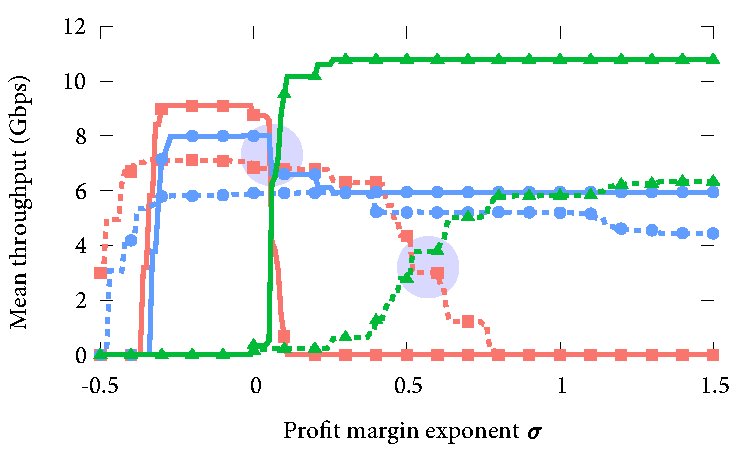
\includegraphics[width=\textwidth]{results/beta-ton.pdf}
        \caption{Throughput as a function of Internet-based cost exponent $\sigma$.}
        \label{fig:ton-beta}
    \end{subfigure}%
    ~ %add desired spacing between images, e. g. ~, \quad, \qquad etc.
      %(or a blank line to force the subfigure onto a new line)
    \begin{subfigure}[b]{0.50\textwidth}
        \centering
        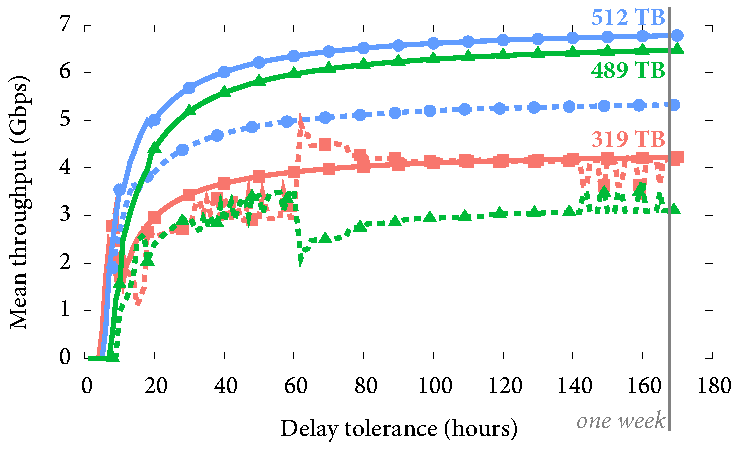
\includegraphics[width=\textwidth]{results/delayTolerance-ton.pdf}
        \caption{Throughput as a function of delay tolerance $\tau_{st}$.}
        \label{fig:ton-delayTolerance}
    \end{subfigure}
    
    \begin{subfigure}[b]{0.50\textwidth}
        \centering
        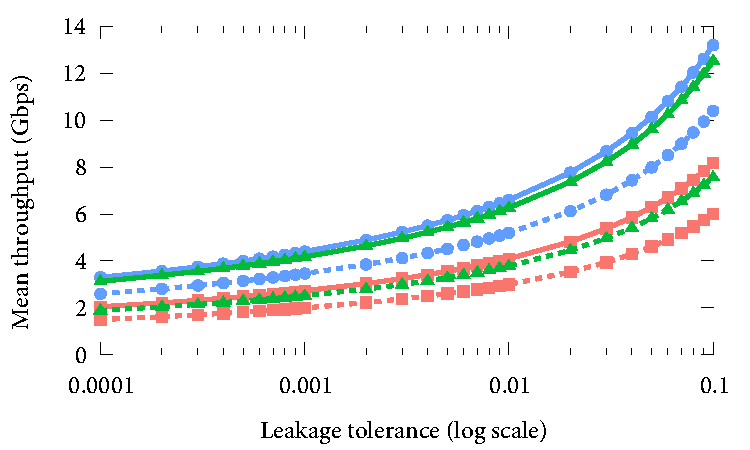
\includegraphics[width=\textwidth]{results/leakageTolerance-ton.pdf}
        \caption{Throughput as a function of leakage tolerance $l_{st}$.}
        \label{fig:ton-leakageTolerance}
    \end{subfigure}%
    ~ %add desired spacing between images, e. g. ~, \quad, \qquad etc.
      %(or a blank line to force the subfigure onto a new line)
    \begin{subfigure}[b]{0.50\textwidth}
        \centering
        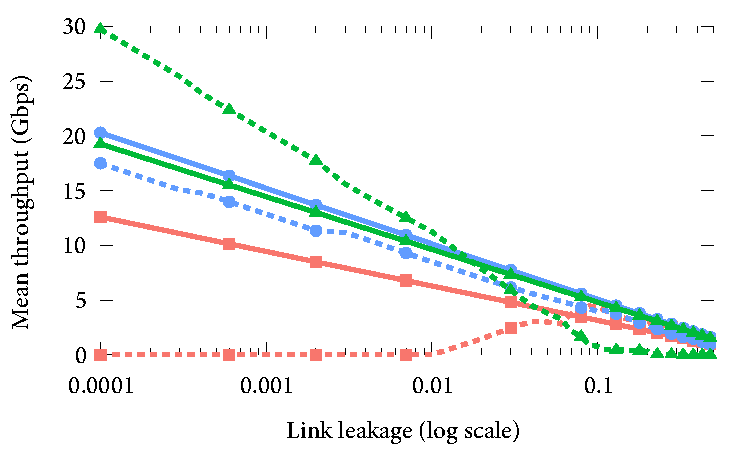
\includegraphics[width=\textwidth]{results/linkLeakage-ton.pdf}
        \caption{Throughput as a function of logical link leakage $l(i,\,j)$.}
        \label{fig:ton-linkLeakage}
    \end{subfigure}
    \caption{Evaluation results with, by default, delay tolerance $\tau_{st} = 96$~hours, leakage tolerance $l_{st} = 0.01$, logical link leakage $l(i,\,j) = 0.05$ for all offloading demands $d_{st}$. The values of the Internet-based cost $\sigma^{\text{rep}}$ and $\sigma^{\text{nrep}}$ are chosen such that the standard deviation of the throughput of all flows is minimized, to ensure fairness among competing data offloading demands.}
    \label{fig:ton-evaluation}
\end{figure*}

In Figure~\ref{fig:ton-evaluation}, we first note that the \textit{rep} model (with solid lines) always achieves better throughputs than the \textit{nrep} model (with dashed lines). Indeed, the \textit{nrep} model takes into account all logical link leakages in the paths it considers and replicates the data accordingly, sending more data than the \textit{rep} model. We also note that our offloading infrastructure can achieve transfers with a throughput above 10~Gbps and aggregated data transfers in the Petabyte range with the \textit{rep} model within a week (\ie as shown in Figure~\ref{fig:ton-delayTolerance}: 512~TB transferred within a week for demand $d_B$, 489~TB for $d_C$, and 319~TB for $d_A$ amounts to 1,320~TB transferred within a week).

Figure~\ref{fig:ton-beta} represents the evolution of the throughput of the three demands as a function of $\sigma$, given the delay tolerance, the leakage tolerance, and the logical link leakage. We note that the value of $\sigma$ is decisive concerning the allocation of the flows to favor: either short distance (demand $d_A$) or long distance (demands $d_B$ and $d_C$). This behavior happens in both \textit{rep} and \textit{nrep} models, although the breaking points (represented by circles in the plot) are not the same for the two models: the break happens at $\sigma = 0.06$ for the \textit{rep} model, and $\sigma = 0.6$ for the \textit{nrep} model. Beyond these points, long-distance demands are favored compared with short-distance ones. Indeed, $\gamma_{st}$ is a factor in the maximization objective (defined in Section~\ref{sec:revenue-maximization}) and the higher the $\gamma_{st}$, the bigger the total revenue we aim to maximize. As shown in Figure~\ref{fig:demand-price-km}, since $\sigma$ is the exponent of the Euclidean distance between $s$ and $t$, we have:

\begin{itemize}

	\item If $\sigma < 0$, $\gamma_{st}$ decreases when the distance increases, favoring short-distance offloading demands.

	\item If $\sigma = 0$, $\gamma_{st} = 1$, favoring short-distance demands with a lower average travel time between the source and destination.

	\item If $\sigma > 0$, $\gamma_{st}$ increases with the distance, favoring long-distance offloading demands.

\end{itemize}

Although the impact of $\sigma$ on the allocation of the flows between demands $d_A$ and $d_C$ is strong, the impact is weaker with demand $d_B$, as this latter shares few subpaths with $d_A$ and $d_C$, as represented in Figure~\ref{fig:allocation-subpaths-offloading-overlay}. Since we want a fair flow allocation when offloading data, we choose $\sigma^{\text{rep}}$ and $\sigma^{\text{nrep}}$ such that the standard deviation of the throughput of all flows is minimized.

It is important to keep in mind, however, that this allocation has an impact on the total revenue because $\gamma_{st}$ is the factor that generates the revenue. Since $\sigma^{\text{rep}} < \sigma^{\text{nrep}}$, the \textit{nrep} model has a revenue that is much larger than the \textit{rep} model. 

\begin{wrapfigure}[13]{o}[0.7\marginparwidth]{6cm}
    \vspace{-15pt}
    \centering
    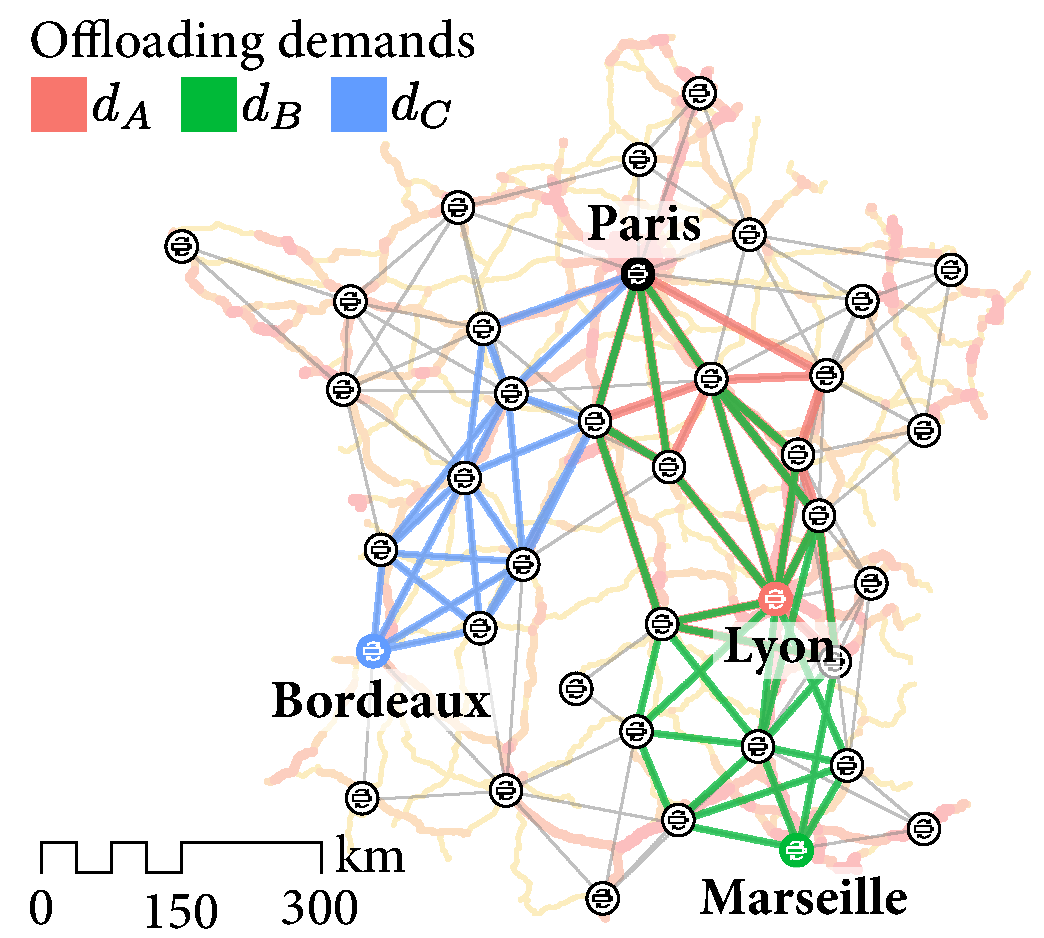
\includegraphics[width=5.4cm]{figures/France-AADT-overlay-layers.pdf}
    \caption{Representation of the logical paths allocated to the three demands $d_A$, $d_B$, and $d_C$.}
    \label{fig:allocation-subpaths-offloading-overlay}
\end{wrapfigure}
Figure~\ref{fig:ton-delayTolerance} shows the throughput as a function of the delay tolerance $\tau_{st}$ (\ie the total duration of the transfer). We notice that the throughput stabilizes as the duration of the transfer increases. For the \textit{rep} model (solid lines), demands with longer distances are favored (demand $d_B$ and $d_C$) over demands with shorter distances (demand $d_A$) Indeed, the total revenue is increased when favoring demands with longer distances, as seen on Figure~\ref{fig:ton-beta}. For the \textit{nrep} model (dashed lines), the allocation of demands $d_A$ and $d_C$ oscillates, favoring one or the other. Both demands have flows allocated on shared subpaths, depending on the maximization of the total revenue. The oscillation results from the variation of the value of $\sigma^{\text{nrep}}$, which depends on the minimization of the standard deviation of the throughput of the allocated flows.

\begin{wrapfigure}[14]{o}[0.7\marginparwidth]{8.5cm}
    \centering
    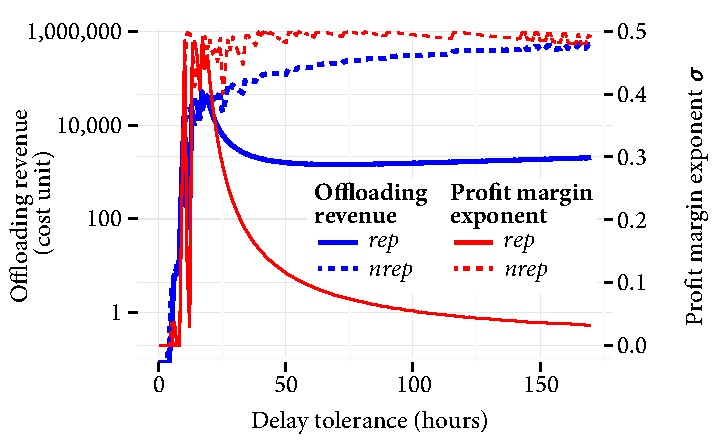
\includegraphics[width=8.2cm]{results/revenue-delaytolerance.pdf}
    \caption{Offloading revenue as a function of the delay tolerance resulting from the allocation of demands $d_A$, $d_B$, and $d_C$, respective to Figure~\ref{fig:ton-delayTolerance}.}
    \label{fig:revenue-delay-tolerance}
\end{wrapfigure}
We represent the offloading revenue (in terms of cost unit) for the allocations of demands $d_A$, $d_B$, and $d_C$ (respective to Figure~\ref{fig:ton-delayTolerance} as a function of the delay tolerance of the offloading demands. Note that the revenue depends on the Internet-based cost and the profit margin exponent $\sigma$. Recall that the latter is chosen for each allocation of the demands given a delay tolerance to guarantee fair allocation of the demands, such that it minimizes the standard deviation of the mean throughput resulting from the allocation of the demands. For this reason,  the resulting offloading revenue is unstable for small delay tolerances (\ie < 50 hours). When increasing the delay tolerance of the offloading demands, the profit margin decreases to guarantee the fairness of the allocations of the demands and the revenue increases. Since more data is transferred, the revenue is becoming less sensitive to the transfer distances and $\sigma$ decreases. Additionally, the revenue resulting from the \textit{rep} model is less than the \textit{nrep} model, as the operational costs when traversing the offloading spots are 1,000 times less for the \textit{nrep} model (since it requires less data to be stored temporarily due to replications).

Finally, Figures~\ref{fig:ton-leakageTolerance} and~\ref{fig:ton-linkLeakage} show the throughput as a function of, respectively, the leakage tolerance $l_{st}$ and logical link leakage $l(i,\,j)$.  The throughput increases when the leakage tolerance increases or the logical link leakage decreases. The \textit{nrep} model almost achieves the same performance, if not better, than the \textit{rep} model when there is a low logical link leakage ($l(i,\,j) < 0.05$). The logical link leakage also has an effect on the allocation of the flows for the \textit{nrep} model when the flows share subpaths, contrary to the \textit{rep} model: shorter distances (demand $d_A$) are favored with a high logical link leakage ($\mathcal{L}(i,\,j) > 0.05$) and longer distances (demands $d_B$ and $d_C$) are favored with a low logical link leakage ($l(i,\,j) < 0.05$). Indeed, the objective function of the \textit{nrep} model depends on the multiplied logical link leakage $l_{p}(i,\,j)$.


\section{Discussion}
\label{sec:discuss}

\subsection{Data security}

The owners of the electric vehicles may try to access the data payload they are carrying. Therefore, the data has to be encrypted so that only the content provider is able to read it. For instance, a public-key infrastructure can be considered (\eg RSA, ECC). The data is encrypted with the public key of the remote entity (the destination of the data) by the originating entity (the source of the data) and will be in turn decrypted by the remote entity using their private key. Also, we can use certificates to authenticate the originating entity of the data by the remote entity.  

Also, we consider a multiple path allocation of the data both on the road infrastructure and on the offloading overlay, which offers path diversity. Therefore, the data that is part of the same flow (or even the same data when replicated) will not take the same path (either road path or logical path). This provides robustness for data transfers, as well as increased security since the data belonging to the same flow will be scattered over multiple paths, making it difficult to attack the whole data transfer by preventing single vantage point attacks.

\subsection{Drayage system}

Recall that data is offloaded from a conventional data network to the closest offloading spot using a drayage system\index{drayage|bb}. The drayage is equivalent to the first and last mile of the access networks in an Internet-based transfer. The drayage can be carried out by different means:

\begin{itemize}
    
    \item \textit{Dedicated lines} (\eg optical fiber channels) can be set up between the different locations that need drayage. This solution would be adapted to connect locations that require continuous large data exchanges. However, it does not fit temporary data exchanges, as it is a costly solution (\eg the sources and destinations of a data transfer are only temporary). 

    \item \textit{Dedicated vehicles} can provide data drayage between the different locations. These vehicles would be equipped with storage and communication capabilities, with the data size and rates greater in magnitude than the common vehicles we consider in this thesis.

\end{itemize}


\subsection{Predicting the future direction of the stopping vehicles and privacy concerns}

For each stopping vehicle, the offloading spot must determine the subsequent offloading spot on the vehicle's route. The offloading service provider stores \textit{anonymously} the previous locations of the vehicles in a historical database to help the offloading spots predict the remaining itinerary of the stopping vehicles. To this end, the service provider can use probabilistic tools, such as Hidden Markov Models~\cite{simmons2006learning}, maximum entropy~\cite{ziebart2008maximum}, or Bayesian networks~\cite{liao2007learning,krumm2006predestination}. The partial trajectories of the vehicles can be known through the successive locations recorded by the navigation system of the vehicles. Note that, the current road traffic in the vicinity of the offloading spot can also help predict the most likely routes vehicles will take~\cite{xue2009traffic}. 

In order to \textit{accurately} predict the future offloading spot the vehicle will visit, the offloading service requires access to the positioning data of the vehicles, which raises some privacy concerns. While it is common for car manufacturers to collect and analyze such data (\eg Tesla collects the current location of the vehicles for remote vehicle analysis\footnote{https://www.tesla.com/about/legal}), we are aware of the privacy breach this represents for both the driver and passengers. In Section~\ref{sec:business-model}, we presented a ``get paid to drive'' program offered by the offloading service provider to the vehicle owners in exchange for transporting a storage device. With this incentive, some drivers may be more willing to share their positioning data with the service.  Otherwise, the offloading service provider could use the historical visit of the vehicle at charging stations (operated by the charging station operator) to infer the vehicles' future visits based on probabilistic tools (\eg Markov chains).

When the drivers do not want to share any data at all with the offloading service, the offloading spots discard the vehicles that do not share their positioning data because there is no means to predict where they will go next. In this case, these vehicles should not be involved in the data offloading.

\section{Conclusion}
\label{sec:revenue-maximization-conclusions}

In this chapter, we presented the concept of offloading data traffic onto the road network. This concept exploits the existing mobility of vehicles to extend the capacity of conventional data networks such as the Internet. We assessed this concept by comparing the cost of using the road network to transfer data with the cost of transferring the same amount of data on the Internet. To determine the road path providing similar performance in terms of delay and bandwidth as in the case of the Internet, we proposed an allocation model that maximizes the cost-benefit of offloading traffic on the road network over conventional data transfers. To solve this model in reasonable computational time, we proposed a road map reduction procedure which produces a simplified logical representation of the road network.  
%We used data replication the offloading spots to provide reliable data transfers. 
We evaluated this allocation model on the main roads of France using actual road traffic counts. Our results show that the road network can accommodate simultaneous data transfers with an aggregate capacity in the Petabyte range per week.

% In this chapter, we character defined the revenue maximization problem that maximizes the cost-benefit achieved by the offloading service content providers offload data transfers on the road network compared to the use of infrastructure-based networks. We then devise two models derived from two data replication strategies at the offloading spots. With the first replication strategy \textit{rep}, each offloading spot on the allocated logical paths of the data transfers replicates data on multiple vehicles. With the second replication strategy \textit{nrep}, the data is replicated at the source of the transfer and no data is replicated at the intermediate offloading spots. In both cases, the amount of data to replicate at the offloading spots depends on the logical link leakage and it achieved such that the leakage tolerance of the offloading demands is satisfied. We evaluated each of the revenue maximization models on the road network of France. Our offloading service allows data transfers in the Petabyte range per week with a market share of 20\% and only one Terabyte of storage per vehicle. These results confirm the offloading potential of our service, which can help operators handle large amounts of data.
% \chapter{Centralized control of the offloading infrastructure}
\label{cha:vehicular-offloading-service}

In this chapter, we propose an architecture  that leverage the advantages of the logical centralization provided by SDN\index{Software Defined Networking (SDN)|)} to enable efficient control of the road infrastructure to offload bulk delay-tolerant data from an infrastructure network. SDN provides the logistics including planning, implementing, and controlling for the effective and efficient transportation of data over the road network.  

%Our offloading service relies on private vehicles equipped with storage devices combined with the use of offloading spots which refer to wireless data storage devices located where vehicles park as part of their line of travel. Figure~\ref{fig:taxonomy} gives an overview of the operations involved in the offloading of large amounts of delay-tolerant background data over the road network between two remote data centers. We target long-lived data transfers lasting several days to a few weeks. These transfers result from provisioning or maintenance activities across remote data center sites, typically required for virtual machine migrations or offline backups. 

%As a result of the data transfer allocation, the offloaded data follows the allocated paths traveled by the vehicles on the roads connecting the successive offloading spots involved in the data transfers. 

We propose a centralized architecture for flexible and scalable configuration of the network of offloading spots. We use the SDN (\textit{Software-Defined Networking}) paradigm, which provides the logistics for efficient and effective vehicular transportation of data. Our SDN-controlled architecture consists of a central controller and a collection of offloading spots. 
%The controller receives demands to offload data transfers onto the road network. An offloading demand indicates the source and destination of the transfer as well as its performance requirements (\eg in terms of delay and bandwidth). 
The controller is in charge of mapping a data transfer onto a sequence of offloading spots matching the direction of a vehicle against the destination of the data.

To enable efficient data offloading, our architecture needs to be designed so to cope with the high degree of complexity of the road network topology and the large number of daily routine journeys involving vehicles. This lead us to propose a road map reduction procedure which produces a logical representation of the road network infrastructure. This representation will be used as an input for the data transfer allocation procedure presented in Chapters~\ref{cha:feasibility-study} and~\ref{chap:implementation}. Each formulate the allocation procedure problem according to two linear programming (LP) models that maximizes the cost benefits that result from using vehicles as data carriers and maximizes the road traffic utilization, respectively. 
%Updates of allocation decisions are also required for maintaining high utilization in face of changes in the road traffic.

%Firstly, our architecture needs to have a global view of the flows of vehicles so to efficiently assign them the data transfers. The offloading spots then use the output of the allocation to decide which data to load or unload from the stopping vehicles. Secondly, this architecture must be scalable to make the data transfer allocation problem tractable. To this end, it must mitigate the complexity of the road network topology and the large number of vehicular trips.

Our main contributions in this chapter are the following two:
\begin{itemize}

    \item \textbf{Centralized architecture.} We present a centralized architecture that enables scalable and adaptive control of the road network to offload traffic. This architecture also provides the control to guarantee reliable data transfers.
    
    \item \textbf{Road map reduction.} We propose a mapping algorithm which produces an  offloading overlay, a logical representation that characterizes the movements of the vehicles into network quantities. The offloading overlay mitigates the complexity of the road network and makes the data transfer allocation problem tractable.
    
    %\item {\bf Road network resource allocation.} We design an allocation procedure that selects vehicle flows to match the performance requirements of offloading demands.
    	
\end{itemize}

This chapter is structured as follows. In Section~\ref{sec:overview-service}, we present an overview of our offloading service by introducing the reference scenario we will use throughout the thesis. In Section~\ref{sec:offloading-system-operations}, we present a centralized architecture that draws on the SDN paradigm to enable scalable and adaptive control the road network infrastructure. In Section~\ref{sec:offloading-service-model}, we give an abstract model of the offloading service by which we introduce the notations we will use in the rest of this document. In Section~\ref{sec:mapping-offloading-overlay}, we introduce an algorithm for reducing the complexity of the road network. The output of our algorithm is an \textit{offloading overlay} which gives a logical representation of the road network. The offloading overlay allows us to propose models to allocate data transfers onto the road network.

\begin{figure}[h!]
	\centering
		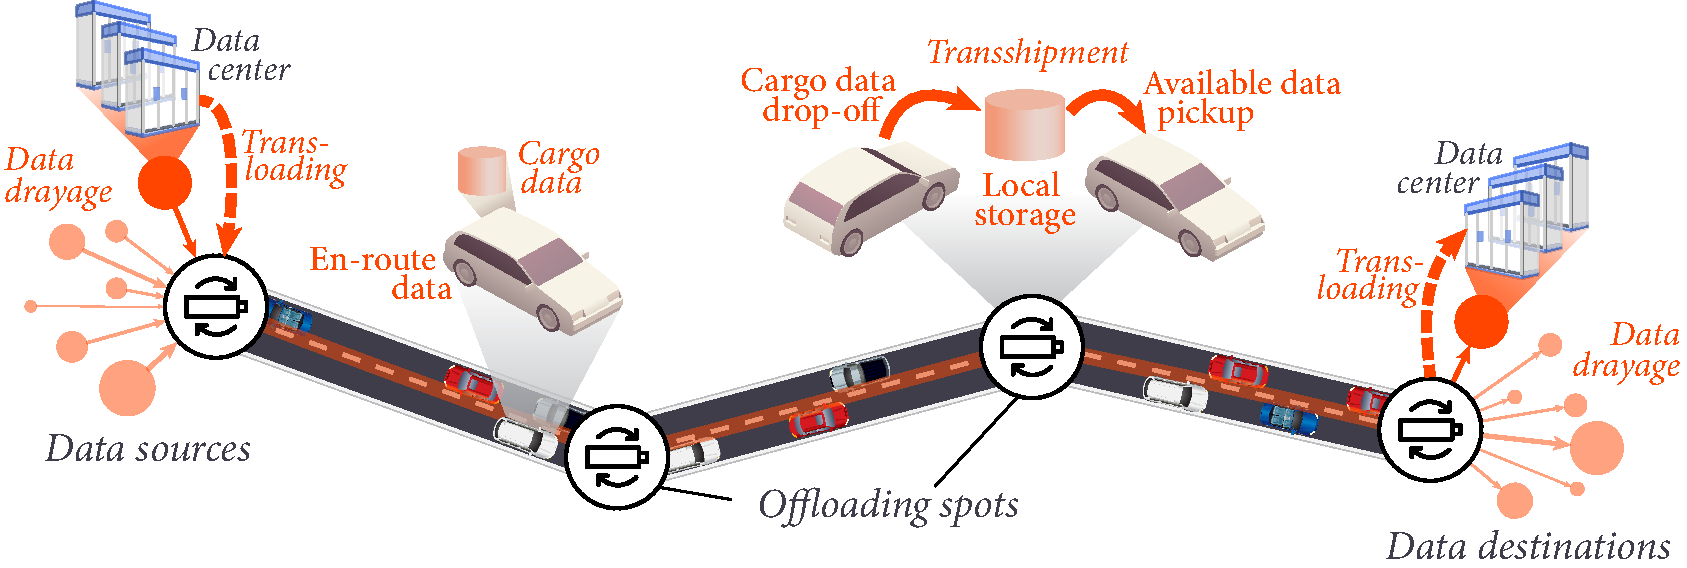
\includegraphics[width=0.75\columnwidth]{figures/taxonomy.pdf}
	\caption{Overview of our road-based offloading service.}
% 	Part or all the data of a transfer between two remote data centers is shifted from the Internet to the road network. Data is first transloaded by means of drayage to the closest edge offloading spot until transferred on empty stopping vehicles. Subsequent intermediate offloading spots act as data relays where vehicles can drop off data on their route for later pick-up and delivery by other vehicles. Once at destination, the data is transloaded back into the data network.}
	\label{fig:taxonomy}
\end{figure}

\section{10,000-foot view of the offloading service}
\label{sec:overview-service}



The decision of loading data on or off vehicles is taken by the offloading spots according to forwarding states installed by an SDN-like controller. The offloading spots act similarly to forwarding engines under the direct authority of the controller. The next section describes the SDN centralized architecture we propose for efficient data offloading onto the road network.   

%The offloading spots act as data exchange relays to compose the trajectories of vehicles traveling in different directions. 
 
%We take advantage of the parking time to opportunistically load on or unload data from vehicles while they are stopped at the offloading spots. The data is \textit{transloaded}\index{transloading} from a conventional data network to the closest offloading spot by means of \textit{drayage}\index{drayage}. 

%The data is stored until transferred to stopping vehicles that will carry it to its destination.

%The offloading service provider\index{offloading service provider|bb}, if different from the vehicle manufacturers, offers a ``get paid to drive'' program to the vehicle owners. The service provider installs the storage devices and the vehicle owners\index{vehicle owner} receives a monthly fee or a discount on the cost of refilling or charging their vehicle in exchange for driving their normal routine. The discount rate is negotiated with the gas station operator\index{gas station operator} (\eg Total or BP) in the case of internal combustion engine vehicles or the charging station operator\index{charging station operator} (\eg ChargePoint or Tesla) in the case of electric vehicles\index{Tesla}. The discount rate is calculated based on the driving pattern including coverage and mileage. If the vehicle manufacturers take on the role of service provider, vehicles are equipped as standard with on-board storage devices and the offloading service is provided without involving nor compensating the vehicles' owners. The service provider charges the content provider\index{content provider} for the amount of data to offload on the road network and shares the revenues with the gas or charging station operator\index{charging station operator}.


\section{Centralized controlled offloading architecture}
\label{sec:offloading-system-operations}

We leverage the advantages of the logical centralization provided by \acrfull{sdn}\index{Software-Defined Networking (SDN)} to enable efficient control and management of the road network resources to offload bulk delay-tolerant traffic from a conventional data network. Following \acrshort{sdn}'s original design, our architecture consists of two components, as depicted in Figure~\ref{fig:architecture}: a central controller\index{controller} and the offloading spots acting as forwarding entities. We describe the function of each component in the remainder of this section and evaluate the benefits of the central controller in Section~\ref{sec:need-for-controller}. 

\begin{figure}[t]
	\centering
	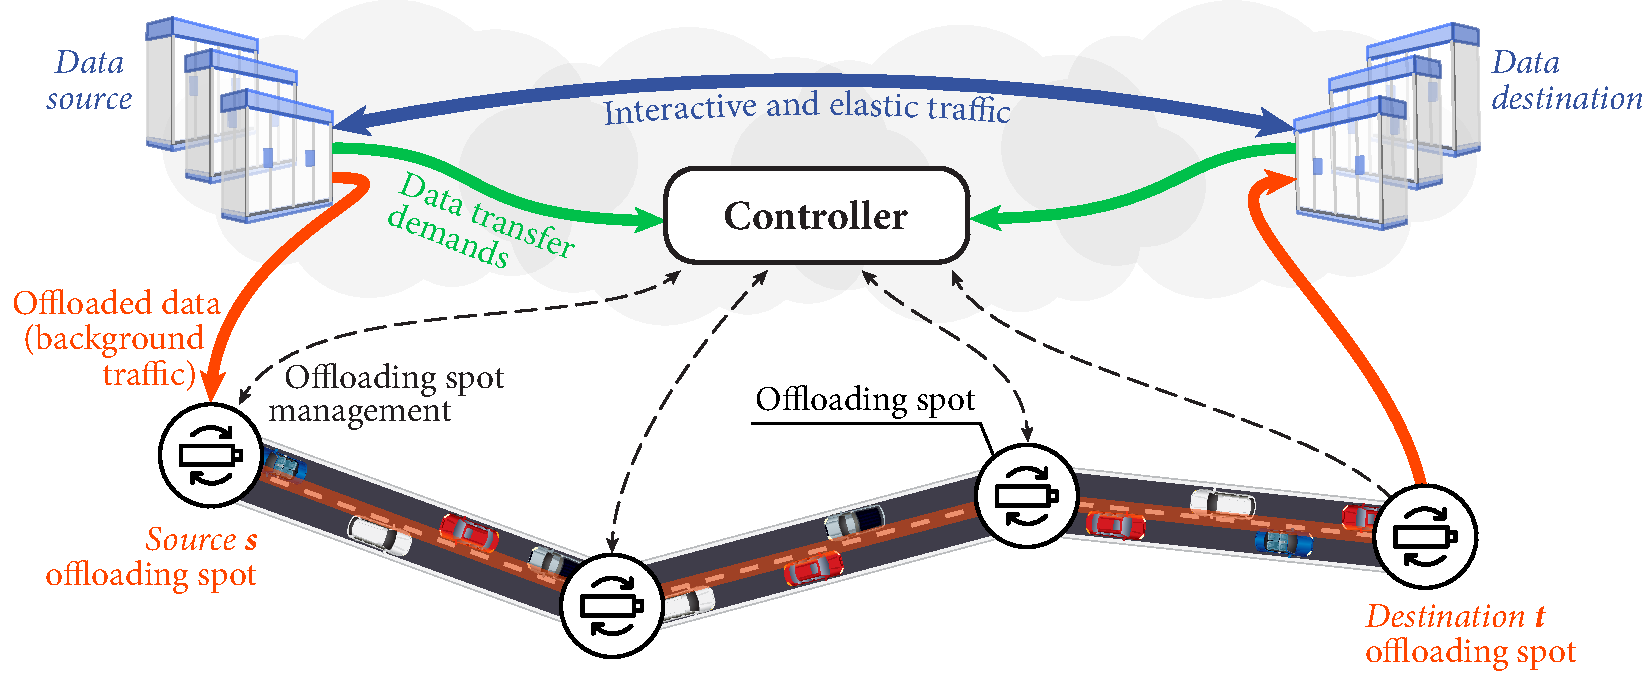
\includegraphics[width=0.75\columnwidth]{figures/architecture2.pdf}
	\caption{Centralized architecture for the offloading service.}
% 	In this scenario, the controller receives demands to offload bulk transfers of delay-tolerant data between two data centers. The controller configures the road network data plane by installing forwarding states at the offloading spots. The controller allocates the flows of vehicles on the roads connecting the offloading spots to carry the data towards its destination.}
	\label{fig:architecture}
\end{figure}

\subsection{Controller}

The controller\index{controller|bb} has a holistic knowledge of the road network including its topology and dynamics, such as the traffic volumes for each road segment. Such knowledge may be derived from traffic forecasting services such as Navteq/Here\footnote{\url{https://www.here.com/business/traffic}},     
TomTom\footnote{\url{http://automotive.tomtom.com/en/connected-services/tomtom-traffic}}, or 
Airsage.\footnote{\url{http://www.airsage.com/Products/Traffic-Insights/}}. The controller keeps track of the status of the offloading spots via a long range control channel (\eg SIGFOX\footnote{\url{http://www.sigfox.com/}}). The information about the offloading spots includes the metadata of the data in transshipment and the statistics about the stopping vehicles, including the historical locations' made available via the navigation system of the vehicles. By collecting the information about the offloading spots, the controller has an up-to-date view of the offloading system. In Section~\ref{sec:discuss}, we present a list of probabilistic tools for inferring the remaining route of a vehicle knowing its navigation history.       

The controller receives demands\index{offloading demand} to offload data from transfers on the road network. Each demand specifies the delay and bandwidth requirements for the corresponding data transfer, as well as the origin and destination. When receiving an offloading demand, the controller selects the road network paths by solving the data transfer allocation problem\index{data transfer allocation problem}. A road network path consists of a sequence of offloading spots followed by the data carried by vehicles between the offloading spots. We formulate the data transfer allocation problem as two linear programming (LP) models. A first one is the revenue maximization problem we present and solve in Chapter~\ref{cha:feasibility-study}. A second one formulates the allocation as the throughput maximization problem in Chapter~\ref{chap:implementation}. In both models, the data transfer allocation problem determines the road networks path and also how much data to allocate to the flows of vehicles traveling between the consecutive offloading spots along the road network paths. 

Figure~\ref{fig:controller-flowchart} shows the interactions between the functions of the controller with those of the offloading spots. The allocation procedure involves a reduction of the road network with the offloading overlay we detail in the next section. 

\begin{figure}[t]
	\centering
		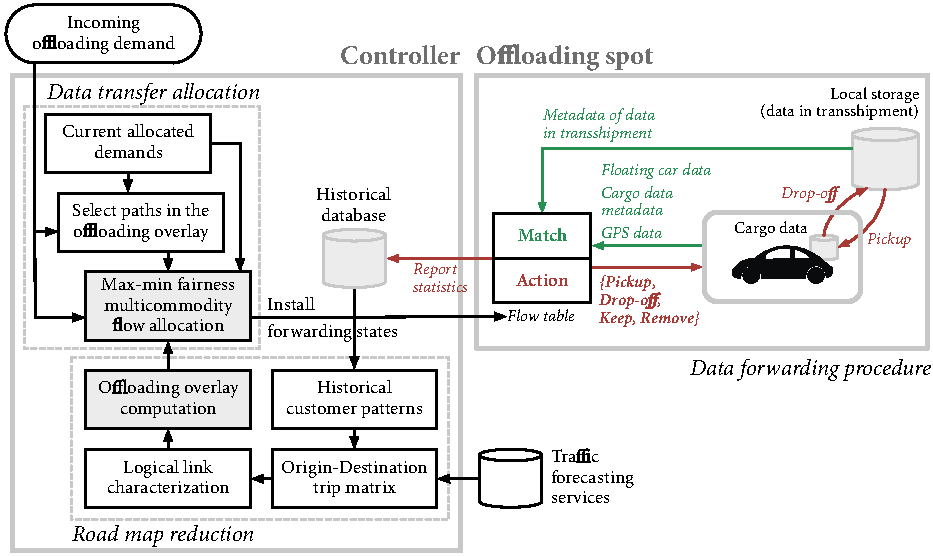
\includegraphics[width=\columnwidth]{figures/controller-flowchart-offloading-spot.pdf}
	\caption{Interactions between the functions of the controller and those of the offloading spots.}
	\label{fig:controller-flowchart}
\end{figure}


\subsection{Data forwarding at the offloading spots}
\label{sec:data-forwarding-offloading-spot}

We represent the interactions between the actions of the controller and the offloading spots in Figure~\ref{fig:controller-flowchart}. The controller installs forwarding states to control the local decisions made at the offloading spots to either drop off or pick up the data cargo. This decision results from the matching of the direction of the stopping vehicles against the destination of the available data. The local decisions account for the allocation of the road network resources shared among concurrent offloaded data transfers.

\begin{wrapfigure}[24]{o}[0.7\marginparwidth]{7.6cm}
    \includegraphics[width=7.5cm]{figures/forwarding.pdf}
    \caption{Forwarding process at an offloading spot.}
    \label{fig:forwarding-process}
\end{wrapfigure}
\paragraph{Flow tables.} 
The forwarding behavior of an offloading spot is determined by its \textit{flow table}\index{flow table|bb} represented in Figure~\ref{fig:controller-flowchart}. It consists of a list of entries, each installed for an individual offloading demands. The controller adds a new entry in the flow table of all the offloading spots on the road network path resulting from the allocation of a data transfer.
A flow entry contains the next-hop offloading spot to forward the data car along the allocated road path toward its destination.
% A flow entry forwards the data cargo to the next-hop offloading along the computed road path toward its destination.
% A flow table entry contains the next-hop offloading spot to which the data must be forwarded to reach the destination of the data transfer corresponding to this entry. 
The destination of the stopping vehicles is matched against the next-hop offloading spot of the flow entries. If there is a match, the offloading spot performs an action described by the forwarding process.
% on the cargo carried by the vehicle associated with the entry, including loading data on or off the vehicles.

\paragraph{Forwarding process.} 
The forwarding process is represented by the flowchart depicted in Figure~\ref{fig:forwarding-process}. Upon the arrival of a vehicle, an offloading spot checks if the direction of the vehicle matches one entry of its flow table. If none of the entries match, the vehicle unloads, if any, its data cargo onto the offloading spot storage for future pick-ups and continues its journey without performing any further actions. If multiple entries match the direction of an empty vehicle, the offloading spot selects one entry based on the scheduling strategies presented in Section~\ref{sec:scheduling}. After selecting one of the entries, the offloading spot performs the actions specified in the entry. If the vehicle already carries data, the offloading spot checks if this data belongs to the data transfer represented by the matching entry. If this is the case, the vehicle keeps its cargo and continues its journey. Otherwise, the vehicle unloads its cargo at the offloading spots before resuming its journey. In case the vehicle arrives empty, if some data matching the vehicle direction is locally available, the data is transferred to the vehicle. Otherwise, the vehicle continues its journey without a cargo. 

\subsection{Evaluating the benefits of a centralized control}
\label{sec:need-for-controller}

To assess the benefits of a central controller, we use a simple scenario composed of four offloading spots as depicted in Figure~\ref{fig:simple-scenario}. We compare different scheduling strategies when concurrent data transfers traverse an offloading spot. Two data transfers $A$ and $B$ originate from offloading spot $S$ and share the road segment connecting offloading spot $I$. The transfers then follow their route toward their final destinations $T_A$ and $T_B$, respectively. 
We only consider the road traffic on the road segments shown in the figure.


\begin{figure}[ht]
    \centering
    \begin{subfigure}[t]{0.4\columnwidth}
        \centering
        % \raisebox{.2\textwidth}{
        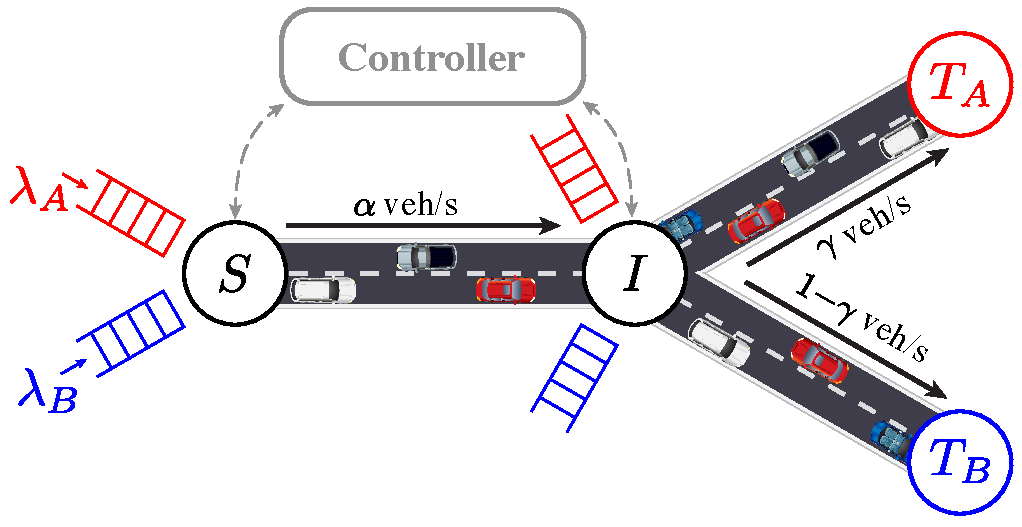
\includegraphics[width=\textwidth]{figures/simpleScenario.pdf}
        % }
        \caption{Two data transfers $A$ and $B$ originating from offloading spot $S$ share the road connecting offloading spot $I$. They then follow their own route toward their final destinations $T_A$ and $T_B$, respectively.}
        \label{fig:simple-scenario}
    \end{subfigure}%
    \quad %add desired spacing between images, e. g. ~, \quad, \qquad etc.
      %(or a blank line to force the subfigure onto a new line)
    \begin{subfigure}[t]{0.47\columnwidth}
        \centering
        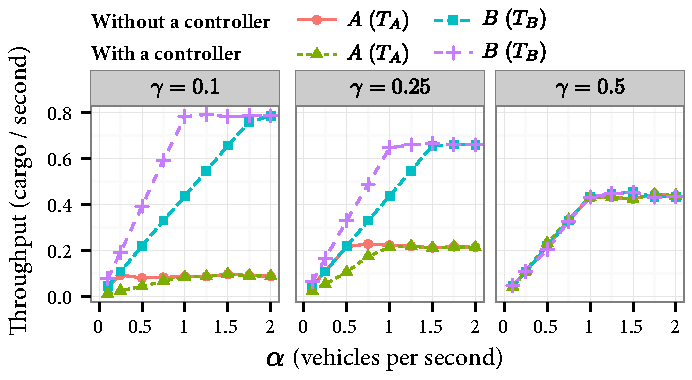
\includegraphics[width=\textwidth]{results/simpleScenario-throughput_v2_gamma.pdf}
        \caption{Maximum throughput (in number of data cargo received per second), for the two strategies with and without controller as a function of parameters $(\alpha,\,\gamma)$.}
        % (deduced from the AADT values)
        \label{fig:simple-scenario-throughput}
    \end{subfigure}
    \caption{Road network consisting of four offloading spots to show the benefits of having a controller.}
\end{figure}

We consider two scheduling strategies, without a controller and with a controller, to select the data transfer and to determine the amount of data to load on the vehicles stopping at each offloading spot. The first scheduling strategy (without a controller) selects the data cargo available at the offloading spots in a round-robin fashion. The data cargo of the transfers is selected in equal proportions and in circular order, without any priority given to the transfers. In the second strategy (with a controller), the decision to load a cargo on a vehicle is based on forwarding states installed at the offloading spots. The controller determines the forwarding states using the traffic volumes of road network under consideration. In the example of Figure~\ref{fig:simple-scenario}, if we assume the road traffic volume $I\rightarrow T_A$ to be three times greater than $I\rightarrow T_B$, the second strategy (with a controller) will load data three times more often onto vehicles heading to $T_A$. This is not the case of the strategy without a controller: this strategy will load the same amounts of data on stopping vehicles regardless of whether they head to $T_A$ or $T_B$.

We use \acrshort{sumo} (\acrlong{sumo})~\cite{behrisch2011sumo} to evaluate the three scheduling policies and simulate microscopic traffic in volumes of $\alpha$ vehicles per second from $S$ to $I$, $\gamma$ from $I$ to $T_A$, and $1 - \gamma$ from $I$ to $T_B$. We assume that both transfers $A$ and $B$ have infinite backlog of data at offloading spot $S$ (\ie $\lambda_A = \lambda_B = \infty$). Figure~\ref{fig:simple-scenario-throughput} shows the throughput of the system measured in the number of data cargo delivered to the destinations per second. In the scenario, the scheduling is relevant at $S$, as the road segments connecting the next-hop offloading spot $I$ to $T_A$ and $T_B$ exhibit different road traffic volumes. We consider an infinite backlog traffic generated at $S$ such that all vehicles leaving offloading spot $I$ are loaded with a cargo.

We can see that, for the first strategy without a controller, the transfer headed to $T_A$ needs a longer ramp-up period to reach its nominal throughput. Without any knowledge on the downstream traffic volumes, $S$ cannot load the optimal amounts of data to the next offloading spot $I$ to fully utilize the network resources. As a result, $I$ does not have enough data locally available to feed the higher flow of vehicles traveling towards $T_B$ compared to destination $T_A$. The resources available on the road segment $(I,\,B)$ remain underused when not enough data belonging to transfer $B$ are transported in an adequate amount to offloading spot $I$, \eg for $\alpha = 2$. On the contrary, the second strategy with controller allows $S$ to load data on vehicles traveling to $I$ in adequate amounts for both transfers. In turn, $I$ has enough data to efficiently utilize vehicles traveling on towards $T_A$ as well as $T_B$. The controller leverages the knowledge of traffic volumes on the downstream road segments to maximize the use of road resources at offloading spot $S$. This second strategy can achieve a better throughput performance for all competing transfers at $I$. 


\section{Road map reduction}
\label{sec:offloading-service-model}

In this section, we present a mapping algorithm that reduces the complexity of the road network. The output of our algorithm is an offloading overlay\index{offloading overlay|bb}, which refers to a logical representation that captures the characteristics and dynamics of the road network. We provide a performance evaluation that measures the reduction factor resulting from the mapping algorithm by comparing the complexity of the offloading overlay over the actual road network.

\subsection{Road network}
\label{sec:road-network-characterization}

We represent the road network\index{road network|bb} by a directed graph $G^R=(N^R,\,L^R)$, where $N^R$ and $L^R$ denote the set of physical nodes and links, respectively. The set of nodes $N^R=N^J\cup N^S$ consists of two subsets: the set of road junctions ($N^J$) and the set of charging stations ($N^S$). A road junction refers to a location where vehicles can change their direction of travel. A link in the road network corresponds to a road segment connecting two adjacent junctions or a junction and a charging station. We consider the road segments and the traffic flowing in both directions homogeneous as they share the same profile in terms of capacity and free-flow speed. For a road segment $(a,\,b)\in L^{R}$, let $v_{ab}$ be its nominal volume of vehicles (vehicles per unit of time), $c_{ab}$ be its capacity (vehicles per unit of time), and $t_{ab}(0)$ be its corresponding travel time at free-flow speed (\ie when $v_{ab}=0$). 

\subsection{Offloading overlay}
\label{sec:offloading-overlay-characterization}

The offloading overlay\index{offloading overlay|bb} provides a logical view\index{logical view} of the road network. More specifically, the overlay mitigates the combinatorial explosion when enumerating the simple road paths in the road network, which becomes
\begin{wrapfigure}[14]{o}[0.7\marginparwidth]{7.5cm}
    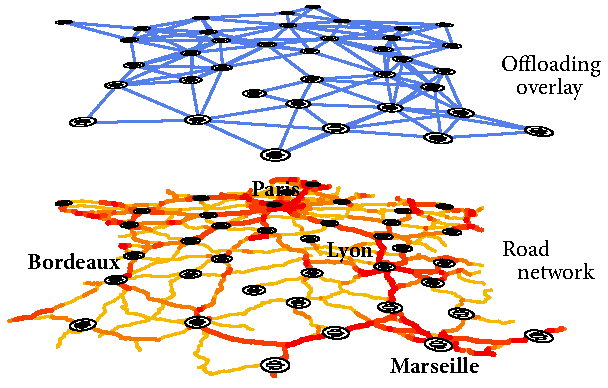
\includegraphics[width=7cm]{figures/France-overlay-1.pdf}
    \caption{The offloading overlay resulting from the deployment plan of offloading spots for the French road network in Section~\ref{sec:charging-station-network} (the width and darkness of the road segments denote the vehicle density).}
    \label{fig:France-overlay}
\end{wrapfigure}
quickly intractable. By providing a logical view\index{logical view} of the vehicle movements on the road paths connecting the offloading spots, the offloading reduces the number of paths to enumerate. 
%and makes the data transfer allocation problem tractable.

We represent the offloading overlay by a directed graph $G^O=(N^O,\,L^O)$, where $N^{O}$ and $L^{O}$ denote the set of logical nodes and links, respectively. A logical node of $N^{O}$ is an offloading spot. A logical link of $L^{O}$ represents the road path (\ie a sequence of road segments) connecting two adjacent offloading spots in the road network. Note that multiple road paths may connect two adjacent offloading spots. In Figure~\ref{fig:France-overlay}, we show an example of realization of an offloading overlay on top of the French road network. 

In the following Section~\ref{sec:characterization-offloading-overlay}, we characterize a logical link $(i,\,j)\in L^{O}$ with network quantities, that is by the weighted travel time $t(i,\,j)$, aggregated capacity $c(i,\,j)$ and data leakage $l(i,\,j)$. The data leakage refers to the loss rate on logical link $(i,\,j)\in L^{O}$ and accounts for the proportion of vehicles that fail to deliver the data to the next offloading spot $j$ because of errors in the prediction of the direction of the vehicle or accidents. We assume that offloading spots are not constrained by the amount of transfers they can serve and have the adequate storage capacity so that the overall service is stable. 
%We evaluate the benefits of the offloading overlay over the raw road network in Section~\ref{sec:complexity-offloading-overlay}. 

\subsection{Mapping algorithm}
\label{sec:mapping-offloading-overlay}

In this section, we present the algorithm we use to map the offloading overlay. We use publicly available datasets with \acrfull{aadt}\index{AADT} for the road segments to characterize the logical links with network quantities. \Acrshort{aadt} is the total volume of traffic traveling on a road segment in both directions for one year, divided by the number of days in the year. The algorithm relies on transportation forecasting\index{transportation forecasting|bb} techniques to translate the traffic counts for the road segments into traffic volumes traveling between the offloading spots. The algorithm proceeds in the steps detailed in the following sections.

\subsubsection{Route determination}
\label{sec:route-determination}

\begin{wrapfigure}[13]{o}[0.4\marginparwidth]{5.5cm}
    \vspace{-10pt}\resizebox{0.9\linewidth}{!}{\begin{tikzpicture}[node distance=2cm]
	\tikzset{
	    bigN/.style={draw,circle,minimum width=0.3cm,inner sep=0},
	    smallN/.style={draw,circle,minimum width=0.3cm,inner sep=0} 
	}
	\node[bigN] (1) at (0,0) {} 
		node[smallN,fill=red] at (1.center) {}
		node at (1.south) [below] {$S$};
	\node[smallN] (3) at (1.5,0.65) {};
	\node[smallN] (2) at (2,-1) {};
	\node[smallN] (4) at (3,-0.5) {};
	\node[smallN] (5) at (3.5,0.25) {};
	\node[smallN] (6) at (4.5,-1.5) {};
	\node[smallN] (7) at (5,1) {};
	
	\node[smallN,dashed] (8)  at (6,2.5) {};
	\node[smallN,dashed] (9) at (6,-1.7) {};
	\node[smallN,dashed] (10) at (7,0.5) {};
	
	\draw (1) -- (2);
	\draw (1) -- (3);
	\draw (1) -- (4);
	\draw (1) -- (5);
	\draw[thick] (1) -- (6);
	\draw[thick] (1) -- (7);
	
	\fill[pattern=custom north west lines,hatchcolor=red] 
		  (-30:5cm) -- (-30:5.5cm)
	      arc (-30:30:5.5cm) -- (30:4.5cm)
	      arc (30:-30:4.5cm) -- cycle;
	\fill[red] 
		  (-30:5.5cm) -- (-30:6cm)
	      arc (-30:30:6cm) -- (30:5.5cm)
	      arc (30:-30:5.5cm) -- cycle;
	\draw[red] (1) -- (-30:6cm) 
		node [pos=0.82,below,sloped] {\textit{refill}};
	\draw[red] (1) -- (30:6cm)
			node [pos=0.4,above,sloped] {Range of the vehicle}
			node [pos=0.98,above,sloped] {\textit{critical}};
	\node[anchor=base west] at ($(-30:6cm) +(0:0.2cm)$) {\textit{Out-of reach}};
\end{tikzpicture}}
\vspace{-5pt}
    \caption{Illustration of the range of a vehicle and the offloading spots within its range.}
    \label{fig:vehicle-range}
\end{wrapfigure}

The first step\index{transportation forecasting!route determination} consists of selecting a subset of the alternative routes connecting each pair of adjacent offloading spots in the road network. Adjacent offloading spots are those within a pre-defined range of the vehicles as shown in Figure~\ref{fig:vehicle-range}. In the case of electric vehicles, the range is limited to the autonomy of the battery. Current electric vehicles have an autonomy of 300~km on average (\eg up to 473~km for the Tesla Model S 90D\footnote{\url{https://www.Teslamotors.com/models}}, 210~km for the Renault Zoe\footnote{\url{http://www.renault.fr/gamme-renault/vehicules-electriques/zoe}}, and 180~km for the Nissan LEAF\footnote{\url{http://www.nissanusa.com/electric-cars/leaf/charging-range/}}). In the case of internal combustion engine\index{internal combustion engine} vehicles, the range is generally higher than electric vehicles. Note that the range of the vehicles highly depends on the driving behavior of the drivers. In the simulations of the following chapters, we considered a conservative vehicle range of 300~km.

The selection of the road paths consists in choosing the paths that are the most relevant to the behavior of the drivers. A natural approach to this problem is to use the All-or-Nothing assignment, which assigns the road traffic to the shortest route between two points~\cite{dijkstra1959note,delling2009engineering,hart1968formal}. While the shortest route may be used by most of the drivers, it does not account for the alternative routes chosen by other drivers, in the case of congestion or road work for instance. To determine multiple routes, on can use algorithms that compute the $k$-shortest routes in terms of travel time~\cite{yen1971finding,eppstein1998finding}. However, for large networks, these algorithms yield routes that are most of the time not reasonable and not actually used by the drivers. More recent algorithms try to determine the most reasonable alternative routes between two points~\cite{geisberger2010route,abraham2013alternative}. In the evaluations of Chapter~\ref{chap:implementation}, we use the algorithm proposed by Abraham \etal~\cite{abraham2013alternative} to determine the most reasonable alternative routes in the road network of France. With this algorithm, the routes are selected such that they share a low degree of similarity in terms of road segments in common. 

\subsubsection{Route assignment}
\label{sec:route-assignment}

The second step\index{transportation forecasting!route assignment} consists in assigning weights to the selected routes. The weights give the proportion of traffic $p(k)$ that will use a certain route $k$. If only one route $k$ was selected by a shortest-path algorithm, then, all the road traffic is assigned to this route and $p(k) = 1$. However, if a set of road paths were selected in the route determination step, we determine the proportion of traffic to assign to each selected route using route choice and traffic assignment strategies. These strategies determine weights to the selected routes. The values of the weights are determined according to attributes such as the travel time and the distance of the routes. 
\begin{wrapfigure}[15]{o}[0.7\marginparwidth]{7.5cm}
    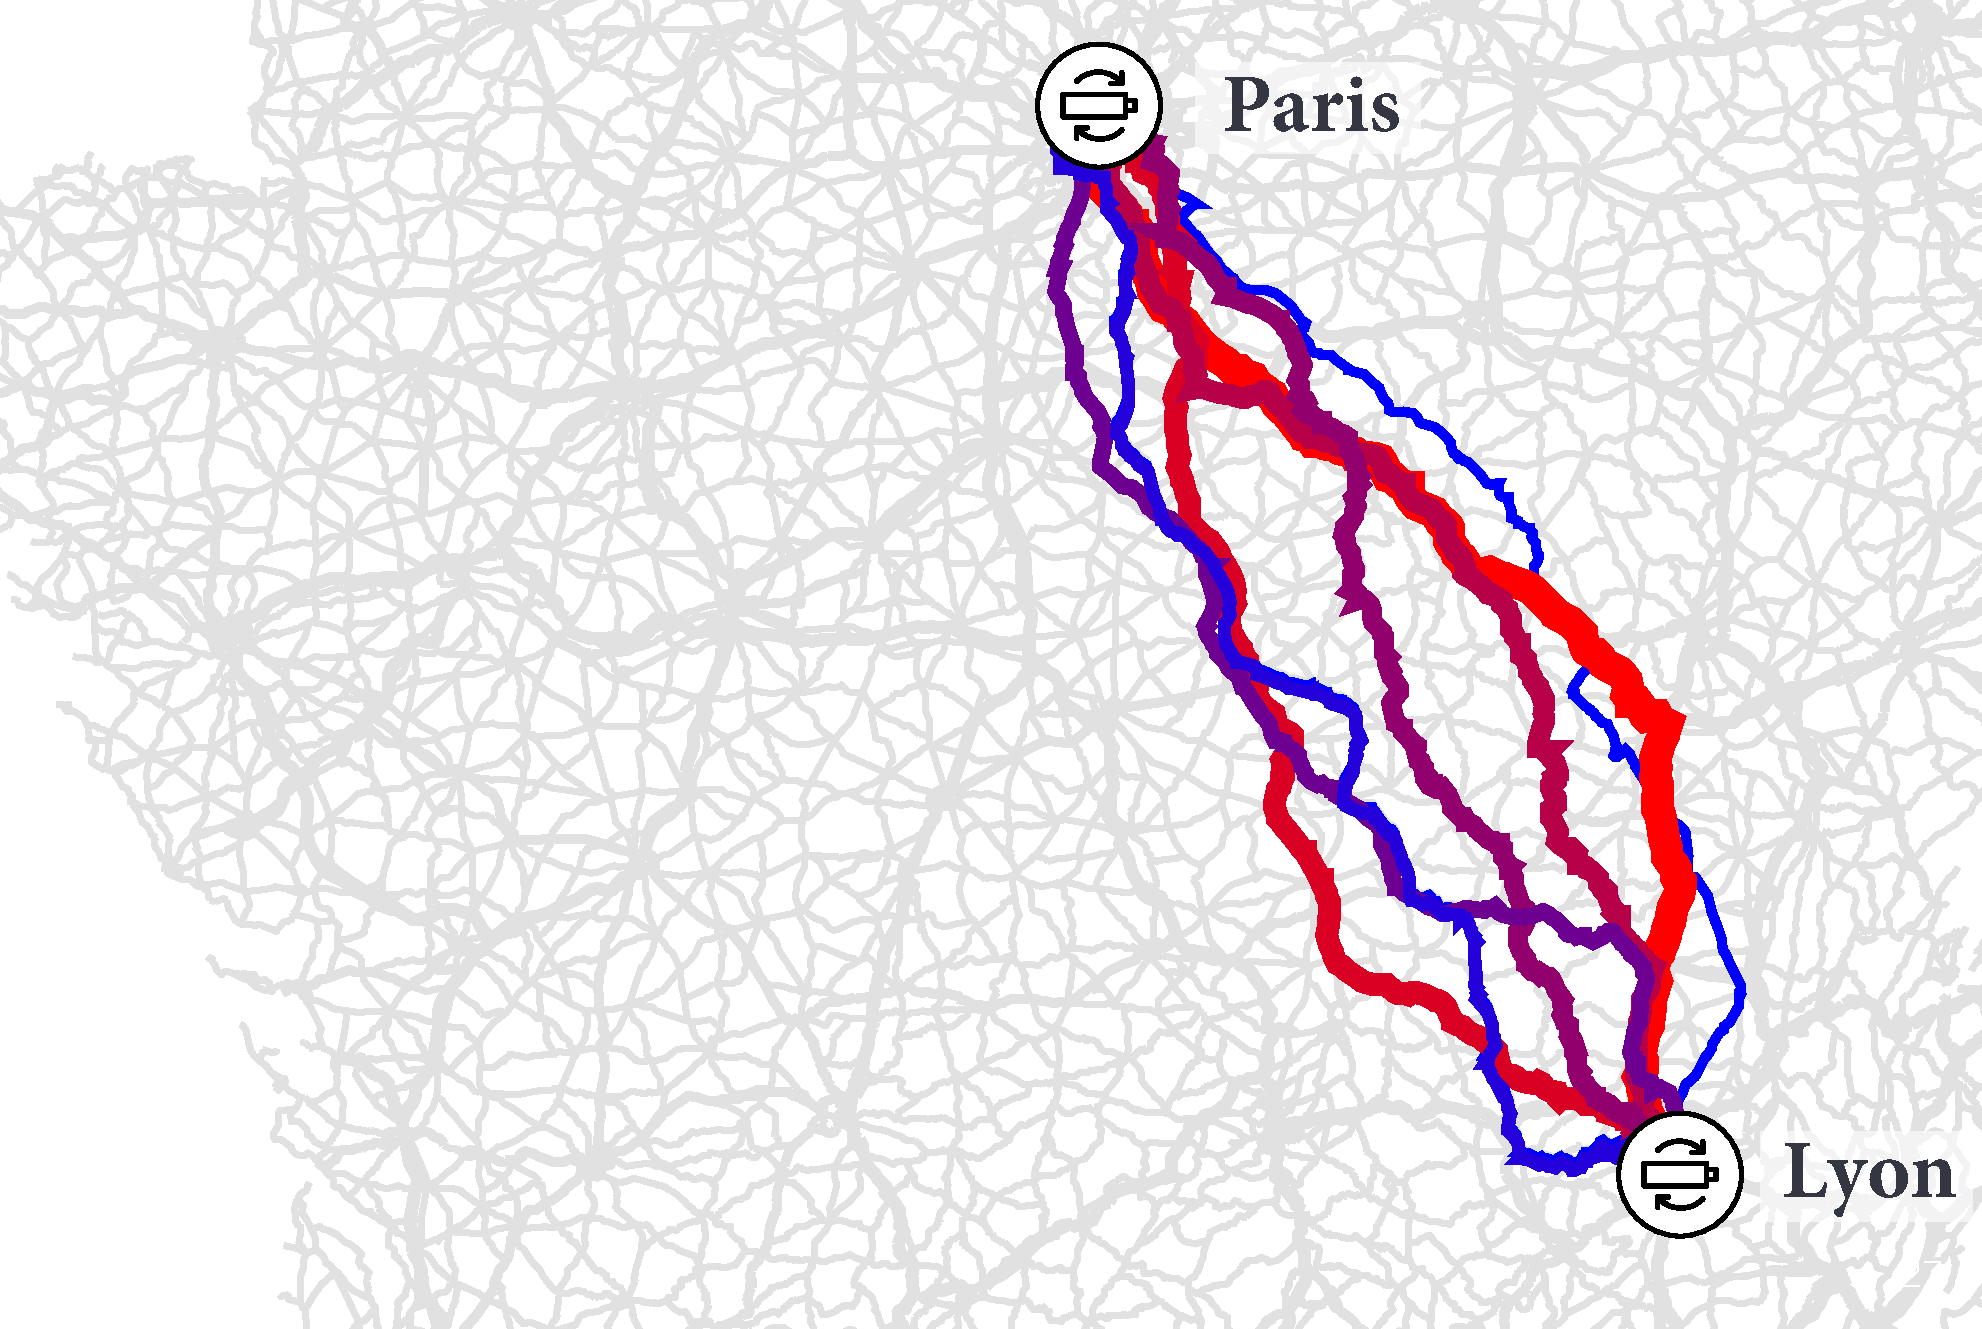
\includegraphics[width=7cm]{figures/route-assignment.pdf}
    \caption{Top 10 routes between Paris and Lyon chosen by the algorithm proposed by Abraham \textit{et al.}~\cite{abraham2013alternative}. The red thickest route is the shortest path and the width of the routes depends on the weights assigned to the routes by the C-Logit traffic assignment~\cite{cascetta1996modified}.}
    \label{fig:route-assignment}
\end{wrapfigure}
Those weights reflect the capacity of a route in attracting traffic, the higher the weight of a route, the more traffic it will receive. To this end, stochastic-user-equilibrium (S-U-E) techniques~\cite{daganzo1977stochastic} were derived from the user-equilibration criterion formulated by Wardrop~\cite{wardrop1952some}. The user-equilibration criterion specifies the following two principles:
\begin{enumerate}
    \item In an equilibrated network, users cannot improve their travel time by changing routes.
    \item The average journey time of all drivers is at a minimum.
\end{enumerate}
The S-U-E techniques build on Wardrop's principles to propose stochastic route assignment algorithms. These techniques include Dial's or C-Logit stochastic traffic assignments~\cite{dial1971probabilistic,cascetta1996modified}.  In the evaluations of Chapter~\ref{chap:implementation}, we use the C-logit route assignment model~\cite{cascetta1996modified} to determine the weights on the selected routes in the road network of France. The C-Logit traffic assignment is a multinominal logit model that assigns a choice probability $p(k)$ on a path $k$ using a perceived utility $U_k$ to each path $k$ of the selected paths:
\begin{equation}
U_k = V_k + \varepsilon_k\quad \forall k,
\end{equation}
where $V_k$ is the average or systematic utility of path $k$ (\eg distance or travel time) and $\varepsilon_k$ is the random residual that includes perception errors of the user’s decisions. Here, we consider the utility $V_k$ is the sum of the inverse of the travel time of each road segment in the road path $k$.

The choice probability, or weight, $p(k)$ for path $k$ is expressed as:
\begin{equation}
p\left(k\right)=\frac{\exp\left[V_{k}-CF_{k}\right]}{\sum_{h\in\mathcal{{P}}^{st}}\exp\left[V_{h}-CF_{h}\right]}\Comma
\end{equation}
where the term $CF_{k}$ is the ``commonality factor'' of path $k$, which is directly proportional to the degree of similarity of path $k$ with the other selected paths. Here, we consider the following expression of the commonality factor:
\begin{equation}
CF_{k}=\beta_{0}\ln\sum_{h\in\mathcal{P}^{st}}\left(\frac{L_{hk}}{L_{k}^{1/2}L_{h}^{1/2}}\right)^{\gamma}\Comma
\end{equation}
where $L_{hk}$ is the length of common paths to $h$ and $k$, $L_{h}$ and $L_{k}$ are the lengths of paths $h$ and $k$, respectively, and $\gamma$ is a positive parameter. Typically, $\beta_{0} = 1$ and $\gamma = 1$ or $\gamma = 2$~\cite{cascetta1996modified}.

The weights determined by the traffic assignment techniques are then used in combination with the traffic counts to estimate the traffic volume of the routes selected in the first step between each pair of adjacent offloading spots. 


\subsubsection{Trip matrix estimation}
\label{sec:trip-matrix-estimation}

In the third step\index{transportation forecasting!trip matrix estimation}, we determine the origin-destination trip matrix that characterizes the number of trips between each pair of adjacent offloading spots. This step can be done qualitatively by conducting travel surveys to know the travel habits of the populations within a geographical area. Examples of these national surveys include the \acrfull{nhts} in the United States\footnote{\url{http://nhts.ornl.gov}} and the \acrfull{entd} in France.\footnote{\url{http://www.statistiques.developpement-durable.gouv.fr/sources-methodes/enquete-nomenclature/1543/139/enquete-nationale-transports-deplacements-entd-2008.html} (in French)} These surveys are conducted by governmental agencies about every ten years. The last version of the \acrshort{nhts} dates from 2009 while the last version of the \acrshort{entd} dates from 2008. There is currently a newer version (2016) of the \acrshort{nhts} survey being conducted. A lower bound of an estimate of the road traffic $T_{ij}$ between pairs of locations $(i,\,j)$ corresponds to the traffic volume $v_{ab}$ of the road segment $(a,\,b)\in L^{R}$ with the lowest traffic of the shortest road path $k$ between the two locations (\ie that corresponds to the bottleneck of the road path). The volume is weighted by $w(d(k))$, the proportion of trips accounted in travel surveys of the same distance as the one of the shortest road path $d(k)$. This estimate can be expressed as follows:
\begin{equation}
    T_{ij} = w(d(k))\times\min_{(a,\,b)\in k}\{v_{ab}\},
\end{equation}

Because these surveys take time and are expensive to conduct, there exist other techniques to estimate traffic matrices between selected locations. These techniques usually rely on \acrfull{aadt}\index{AADT}. It is important to underline that the \acrshort{aadt} is a fundamental statistic used in traffic engineering and transportation planning. The use of the \acrshort{aadt} helps reduce the effects of seasonal bias and missing data mainly due to equipment failure, construction schedules, and installation dates that plague continuous traffic monitoring~\cite{wright1997variability}.

In particular, Zuylen and Willumsen~\cite{van1980most} proposed an entropy-maximizing formulation\index{entropy-maximization problem|bb} to estimate the most likely \acrfull{od} trip matrix\index{origin-destination trip matrix|bb} between the defined locations. The objective of the formulation is to maximize the number of ways of selecting an \acrshort{od} matrix with a total number of trips. As the number of trips increases, the number of ways of selecting an \acrshort{od}  matrix gets more and more peaked and converges to a most likely state. This results in maximizing the entropy of the \acrshort{od}  matrix. The constraint guarantees that the resulting \acrshort{od}  matrix will not overcome the volumes of traffic $v_a$ measured on the road segments $a$. 
\begin{flalign*}
    & \text{Maximize} -\sum_{ij}\big(T_{ij}\log T_{ij} - T_{ij}\big), & \\
    \shortintertext{subject to}
    & v_{a} - \sum_{ij}T_{ij}p^{a}_{ij} = 0 \qquad \forall a \in L^{R}.\\
\end{flalign*}
The probability $p^{a}_{ij}$ denotes the route choice probability of route between source $i$ and destination $j$ to take link $a$ among $S_{ij}$, the set of selected road path. This probability is derived from the choice probability and computed in the route assignment as follows:
\begin{equation}
p^{a}_{ij} = \sum_{\substack{k\in S_{ij}\\k\ni a}} p(k),
\end{equation}
where s.

Since the optimization problem presented above is convex, the authors presented an iterative balancing algorithm to solve it, derive from Bergman's method to solve such problems~\cite{bregman1967proof}. The algorithm is presented in Algorithm~\ref{alg:iterative-balancing}. Each balancing iteration adjusts the quantity $\lambda_{a}$, the road traffic assigned to each road segment $a$. This adjustment is done until all the constraints on the volumes of the road segments are satisfied.
\begin{algorithm}
    \caption{Iterative balancing algorithm for the entropy maximization problem.}
	\DontPrintSemicolon
	\SetKwBlock{Step}{}{}
		
	\Step(\textbf{Step 1.} Initialization){
		$\lambda_{a} \gets 0\quad \forall a\in L$\;
	}	
		
	\BlankLine
	
	\Step(\textbf{Step 2.} Iterative balancing){
		\Repeat{Convergence}{
			$T_{ij}^{\star} \gets \exp\left(\sum_{a}\lambda_{a} \, p^{a}_{ij}\right)\quad \forall i,\,j$\;
			\ForAll{constraints (over domain $L^{R}$)}{
				\If{$V_{a} \neq \sum_{ij}T_{ij}^{\star} \, p^{a}_{ij} $}{
					$\lambda_{a} \gets \lambda_{a} + \ln(V_{a}) - \ln\left(\sum_{ij}T_{ij}^{\star} \, p^{a}_{ij}\right)$
				}
			}
		}
	}
    \label{alg:iterative-balancing}
\end{algorithm}


\subsubsection{Characterization of the offloading overlay} 
\label{sec:characterization-offloading-overlay}

Finally, we characterize the logical links\index{logical link|bb} of the offloading overlay with network quantities, which we determine as follows for each logical link $(i,\,j)$. These network quantities are relevant to solve the data transfer allocation problem.

\paragraph{Travel time $t(i,\,j)$.} 
 The travel time $t{ab}$ of $(a,\,b)$ is given by the \acrfull{bpr} function defined as~\cite{BPR64}:

\begin{equation}
  \label{eq:BPR}
  t_{ab}(v_{ab})=t_{ab}(0)\left[1+\alpha\left(\frac{v_{ab}}{c_{ab}}\right)^{\beta}\right]\Comma
\end{equation}

\noindent where $\alpha$ and $\beta$ are \acrshort{bpr} parameters that depend on the road profile ($\alpha = 0.15$ minutes and $\beta = 4.0$ are typically used)~\cite{HCM00}.

We can deduce from Equation~\ref{eq:BPR} the travel time of physical path $p$, denoted $t_{p}$, which is the sum of all travel times of the road segments that compose the path (we do not consider any turning delays at junctions):

\begin{equation}
  \label{eq:path-delay}
  t_{p} = \sum_{(a,\,b)\in p} t_{ab}(v_{ab}).
\end{equation}

From Equation~\ref{eq:path-delay}, we deduce an expression of the average travel time\index{logical link!average travel time} $t(i,\,j)$ experienced on the $r$ physical paths between nodes $i$ and $j$, weighted by the road traffic flow $v_{p}$ on each path $p$:

\begin{equation}
  \label{eq:ovelray-link-delay}
  t(i,\,j) = \frac{\sum_{p\in S_{ij}} t_{p}\,v_{p}}{r\sum_{p\in S_{ij}}v_{p}}\Comma
\end{equation}

\noindent where $S_{ij}$ is the set of all simple physical paths between $i$ and $j$ (\ie with no cycles in the path).

\paragraph{Capacity $c(i,\,j)$.}
The capacity\index{logical link!capacity} $c(i,\,j)$ of the overlay link $(i,\,j)\in L^{O}$ depends on the sum of the traffic flows $v_{p}$ of the simple paths between offloading spots $i$ and $j$ (\ie the number of vehicles per unit of time going from $i$ to $j$ on path $p$). The capacity $c(i,\,j)$ of the overlay link also depends on the market penetration ratio\index{market penetration ratio|bb} $\mathcal{M}$ of the vehicles participating in the offloading service and the storage size\index{storage size} $\mathcal{S}$ on each vehicle. We assume that all vehicles are equipped with a storage device of the same size $\mathcal{S}$.

\begin{equation}
  c(i,\,j) = \mathcal{M} \times \mathcal{S} \sum_{p\in \mathcal{P}^{ij}} v_{p}.
\end{equation}


\paragraph{Leakage $l(i,\,j)$.}
The leakage\index{logical link!leakage} $l(i,\,j)$ (comprised between 0 and 1) of logical link $(i,\,j)\in L^{O}$ represents the proportion of data that is lost between offloading spots $i$ and $j$. The leakage increases as more vehicles carrying data prematurely exit the road (\eg the vehicles may exit the highway before reaching the offloading spot or an accident may have occurred). The leakage depends on characteristics that are inherent to the physical paths mapped in the offloading overlay. Additionally, the leakage accounts for the errors inherent to the scheduling and forwarding at the offloading spots. In the evaluations of both the feasibility study (Chapter~\ref{cha:feasibility-study}) and the realization (Chapter~\ref{chap:implementation}), we measure the impact of the leakage on the performance of the offloading system. In both of these chapters, we propose different approaches to mitigate the effects of the leakage:
\begin{itemize}
    
    \item In Chapter~\ref{cha:feasibility-study}, we tolerate a target leakage (leakage tolerance) resulting from the successive logical links traversed by the data cargo. To satisfy this tolerance, we consider two replications approaches that load each cargo multiple times on vehicles, either at the source of the data transfers or locally at each intermediate offloading spot involved in the transfer.
    
    \item In Chapter~\ref{chap:implementation}, we use redundancy techniques to decrease the effects of the leakage and retransmission techniques to completely recover the losses due to the leakage. The retransmissions of the lost data cargo are done either at the source of the data transfer or at the intermediate offloading spots.

\end{itemize}

\paragraph{Logical path $p$.}
In the data transfer allocation problems of the following chapters, $p$ denotes a logical simple path\index{logical path|bb} (\ie without any cycles) defined as the ordered list of offloading spots connected by logical links. $\mathcal{P}_{st}$ denotes the set of all logical simple paths from $s$ to $t$. We characterize the logical paths by the travel time $t(p)$ and the flow (throughput) $f(p)$ allocated on logical path $p\in\mathcal{P}_{st}$ for a given offloading demand $d_{st}$ resulting from the data transfer allocation problem. The logical path travel time corresponds to the average time it takes to transfer one data cargo from one extremity of the path to the other. Note that its expression depends on the allocation model we consider.


\subsection{Benefits of the offloading overlay}
\label{sec:benefits-offloading-overlay}

In this section, we evaluate the benefits of the offloading overlay over the raw road network in terms of the number of paths to enumerate between two distant locations. To this end, we consider the road network of France and select offloading spots among a set of suitable candidate locations. We then use real traffic counts measured on the road network of France to build and characterize the corresponding offloading overlay. To be consistent with our motivating scenario, and without loss of generality, we assume that the vehicles are electric vehicles with a range of 300~km. Note that we will use the same dataset throughout the evaluations of Chapters~\ref{cha:feasibility-study} and~\ref{chap:implementation}.

\subsubsection{Dataset of French road traffic}

\begin{wrapfigure}[16]{o}[0.7\marginparwidth]{6cm}
    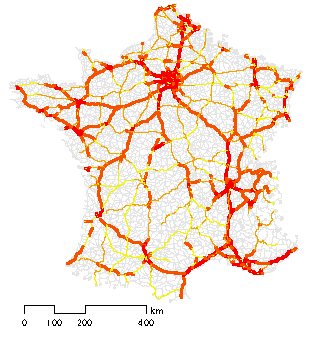
\includegraphics[width=5.7cm]{figures/france-dataset.pdf}
    \caption{Dataset showing the \acrfull{aadt} of the major roads of France in 2011. The road segments have a darker shade when \acrshort{aadt} is higher.}
    \label{fig:france-dataset}
\end{wrapfigure}
Throughout the evaluations we conduct in this thesis, we will use a dataset\index{French road network} collected in 2011 featuring the \acrfull{aadt}\index{AADT} of the major roads in France covering a combined distance of 20,000~km\footnote{\acrshort{entd}~---~Census of the road traffic on the French roads in 2011 (in French): \url{http://tinyurl.com/otfbewv}}.  The traffic volumes are collected using strategically located automatic traffic recorders. The different thickness and shades of red of the road segments depicted in Figure~\ref{fig:france-dataset} reflect the traffic counts given by the \acrshortpl{aadt}. The graph consists of 3,310 edges covering over 20,000~km of roads. 

\subsubsection{Planning of the network of charging stations}
\label{sec:charging-station-network}

We consider a network of charging stations equivalent to the one Tesla\index{Tesla} is currently rolling out in Europe and North America\footnote{\url{https://www.Teslamotors.com/supercharger}}. This network of stations helps electric vehicles face the problem of limited autonomy and achieve long distance travels. Recall that the offloading process will take place in these stations in a transparent manner to the driver. Since there was no such a network in France at the beginning of this thesis, we plan a simple yet realistic network of stations that covers the major roads of France. To plan such a network of stations, we consider a facility-allocation problem\index{facility-allocation problem} that minimizes the number of facilities to allocate, a problem we adapted from the maximal covering location problem~\cite{church1974maximal}. The problem takes demand points and candidate locations as inputs:
\begin{itemize}

	\item The demand points are the 9,555 cities of France with a population greater than 1,000.
   
	\item The candidate locations are the 1,024 Total gas stations, a French oil company.\footnote{\url{http://www.total.fr/mes-deplacements/outils-en-mobilite/export-gps-stations.html} (in French)}

\end{itemize}

\begin{figure}[ht]
    \centering
    \begin{subfigure}[t]{0.4\columnwidth}
            \centering
            % \raisebox{.2\textwidth}{
            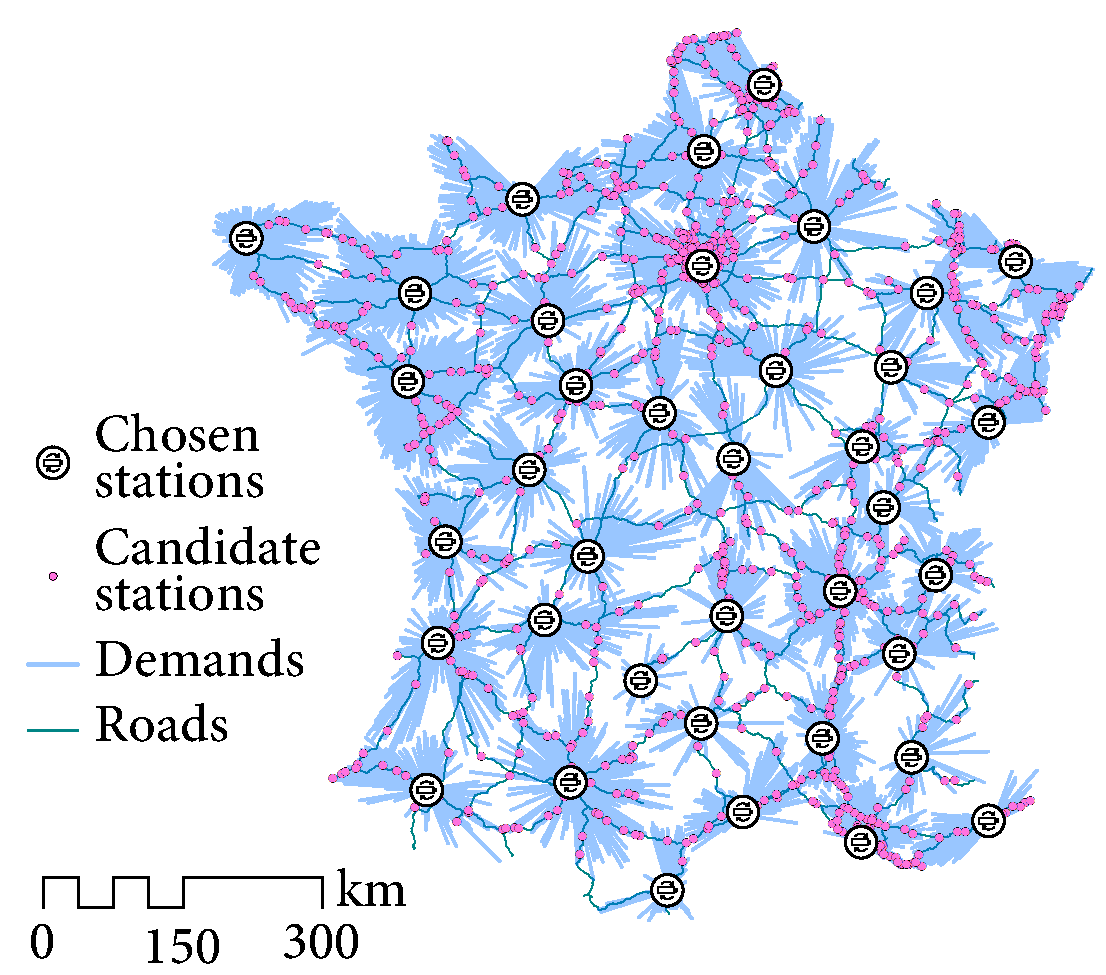
\includegraphics[width=\textwidth]{figures/France-allocation-charging-stations.pdf}
            % }
            \caption{Allocation of charging stations over the French road network. The big dots are the chosen stations, the little dots are the candidate stations, and the lines represent the allocated demands to the chosen stations.}
            \label{fig:France-location-allocation}
    \end{subfigure}%
    \quad %add desired spacing between images, e. g. ~, \quad, \qquad etc.
      %(or a blank line to force the subfigure onto a new line)
    \begin{subfigure}[t]{0.47\columnwidth}
            \centering
            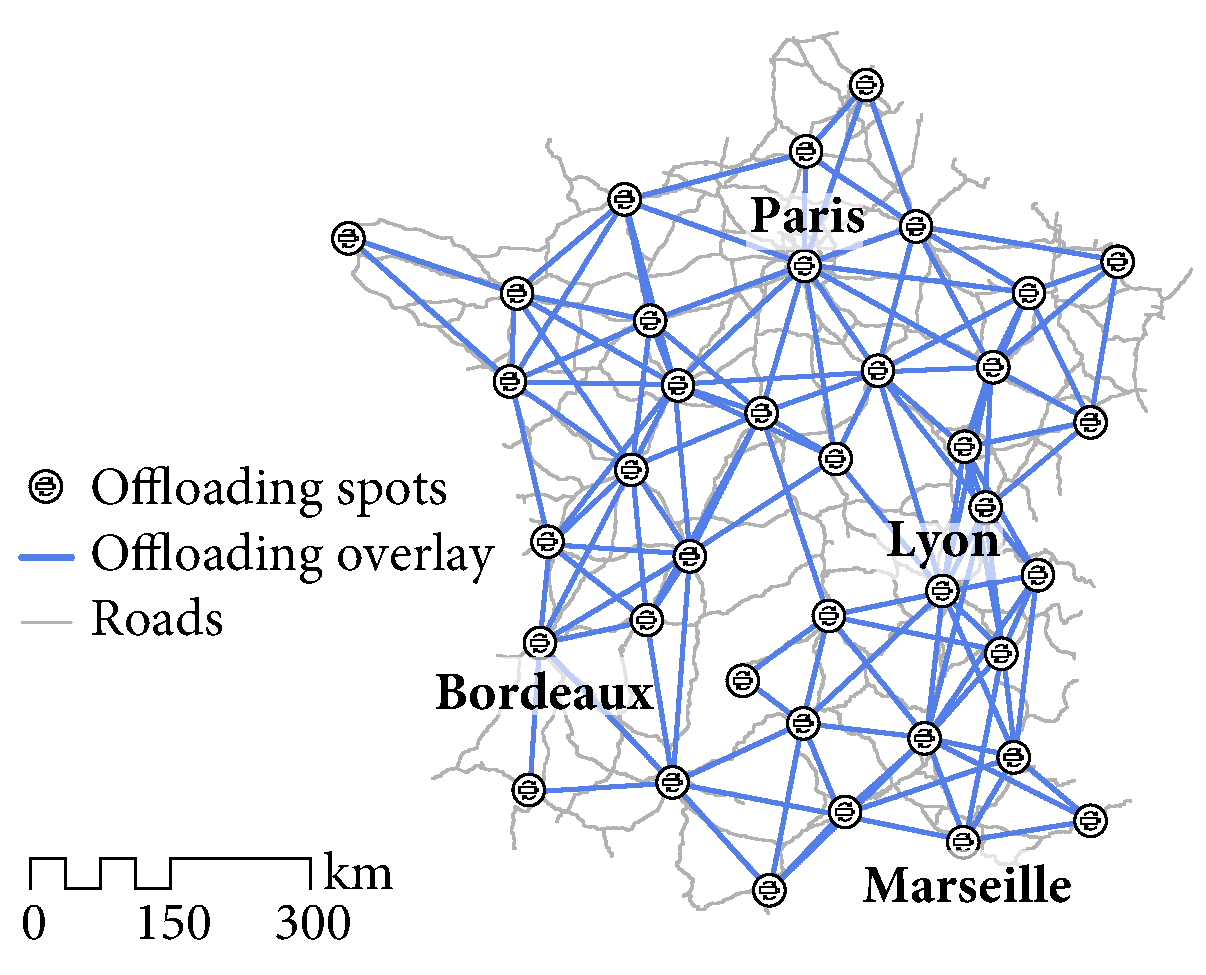
\includegraphics[width=\textwidth]{figures/France-overlay-wo-capacity.pdf}
            \caption{Resulting offloading overlay built on to of the road network of France. The offloading spots are those represented in Figure~\ref{fig:France-location-allocation}.}
            % (deduced from the AADT values)
            \label{fig:France-overlay-wo-capacity}
    \end{subfigure}
    \caption{Facility-allocation result and offloading overlay. The big dots are the chosen stations.}
\end{figure}

The facility-allocation algorithm selects the stations such that a maximum demand points are allocated to the charging stations within a range of 150~km, while minimizing the number of chosen stations. We assume that vehicle ownership is uniform throughout the territory~---~we can then weight the cities by their population. The chosen stations are allocated at most 150~km away from each other. This is enough for a vehicle with an autonomy of 300~km to reach the next closest station or return to the same station without depleting its battery. Finally, we assume that the stations have a capacity that suits the demand such that the waiting time is negligible. The waiting time is then restricted to the service time, which corresponds to the duration of the battery charge.

The resulting allocation outputs 38 stations scattered on the French road network, as shown in Fig.~\ref{fig:France-location-allocation}. We note that the stations are mainly allocated near major cities, as the demand from urban areas is higher than from rural areas.

\subsubsection{Complexity of the offloading overlay}
\label{sec:complexity-offloading-overlay}

The offloading overlay\index{offloading overlay} provides a logical view of the road network. Since the latter is very complex, it becomes quickly intractable to enumerate all the possible simple paths between two distant locations. The offloading overlay allows keeping some of the characteristics of the road network we need to perform our data transfer allocation problem, while reducing the complexity of the initial road network and making the path enumeration tractable. For this evaluation, we aim to show how the offloading overlay compares with the road network in terms of capacity. 

\begin{wrapfigure}[16]{o}[0.7\marginparwidth]{8cm}
    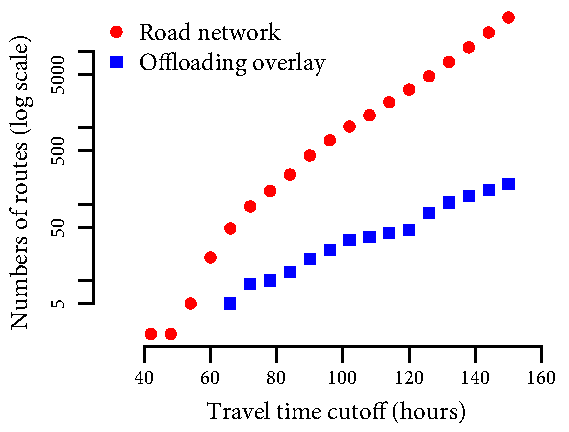
\includegraphics[width=7.5cm]{results/pathcount.pdf}
    \caption{Total number of simple paths in the road network and logical simple paths in the offloading overlay as a function of the travel time cutoff ($y$-axis is in a logarithmic scale).}
    \label{fig:pathcount}
\end{wrapfigure}
To this end, we instantiate an offloading overlay as defined in Section~\ref{sec:offloading-overlay-characterization}. We create it from the network of stations we planned to cover the main roads of France in the previous section. In the offloading overlay representation, the stations become the nodes of the offloading overlay, or offloading spots. The logical links between the stations correspond to the shortest route between two offloading spots. As noted before, we constrain the maximum length of the route to 300~km. The resulting offloading overlay is depicted in Figure~\ref{fig:France-overlay-wo-capacity}. Note that we do not need to fully characterize the logical links of the offloading overlay in terms of capacity to evaluate its benefits. We will fully characterize the logical links when conducting the evaluations in the following chapters.

We plotted the total number of simple paths bounded by a travel time cutoff in both the road network and the offloading overlay. The plot is represented in Figure~\ref{fig:pathcount} and shows the number of all simple paths as a function of the travel time cutoff of the enumerated paths. We note that, in both cases, the number of simple paths grows exponentially with the travel time cutoff. The number of simple paths is much larger on the road network compared to those enumerated in the offloading overlay. Also, the difference in the number of paths grows exponentially. This exponential growth is the main complexity factor to consider when solving the data transfer allocation problem.

\section{Discussions}
\label{sec:discuss}

\subsection{Drayage system}
As shown in Figure~\ref{fig:taxonomy}, data is offloaded from a conventional data network to the closest offloading spot using a drayage system\index{drayage|bb}. The drayage in our services is equivalent to the first and last mile of the access networks in an Internet-based transfer. The drayage can be carried out by different means:

\begin{itemize}
    
    \item \textit{Dedicated lines} (\eg optical fiber channels) can be set up between the different locations that need drayage. This solution would be adapted to connect locations that require continuous large data exchanges. However, it does not fit temporary data exchanges, as it is a costly solution (\eg the sources and destinations of a data transfer are only temporary). 

    \item \textit{Dedicated vehicles} can provide data drayage between the different locations. These vehicles would be equipped with storage and communication capabilities, with the data size and rates greater in magnitude than the common vehicles we consider in this thesis.

\end{itemize}


\subsection{Predicting the future direction of the stopping vehicles.}
For each stopping vehicle, the offloading spot must determine the subsequent offloading spot on the vehicle's route. The controller stores the previous locations of the vehicles in a historical database to help the offloading spots predict the remaining itinerary of the stopping vehicles. To this end, the controller can use probabilistic tools, such as Hidden Markov Models~\cite{simmons2006learning}, maximum entropy~\cite{ziebart2008maximum}, or Bayesian networks~\cite{liao2007learning,krumm2006predestination}. The partial trajectories of the vehicles can be known through the successive locations recorded by the navigation system of the vehicles. Note that, the current road traffic in the vicinity of the offloading spot can also help predict the most likely routes vehicles will take~\cite{xue2009traffic}.

\section{Conclusion}

In this chapter, we introduced the two tools that we will use in the following chapters to allocate the demands to offload data transfers on the road network. 

Firstly, we proposed a centralized architecture with a controller that has a holistic view of the system to manage and configure the offloading spots to match the requirements of demands to offload data. In the following chapters, we rely on this architecture to enable the efficient allocation and reliability of data transfers over the road network. We showed the benefits of the centralized architecture in the resulting throughput over a distributed architecture where the offloading spots take local forwarding decisions.

Secondly, we introduced the offloading overlay as a logical view used by the controller to represent the resources of the road network to mitigate its scale. The nodes of the overlay correspond to the offloading spots and the links characterize the movements of vehicles between the offloading spots as networking quantities relevant to the allocation of the data transfers, including the capacity, travel time, and data leakage. We showed that the offloading overlay effectively decreases the complexity of the main roads of France, as it provides a logical overlay with an exponential difference in the number of paths for given path travel times. 

In the next chapter, we will use both of these tools to assess the feasibility of the offloading service when comparing it to transfers on conventional data networks.
\chapter{Centralized control of the offloading infrastructure}
\label{chap:implementation}


In this chapter, we propose an architecture implementing the vehicular data offloading. We leverage the advantages of the logical centralization provided by \acrfull{sdn}\index{Software-Defined Networking (SDN)|)} to enable efficient control and management of the offloading infrastructure. \acrshort{sdn} provides the necessary logistics including planning, implementing, and controlling for the effective and efficient transportation of data over the road network.  

%Our offloading service relies on private vehicles equipped with storage devices combined with the use of offloading spots which refer to wireless data storage devices located where vehicles park as part of their line of travel. Figure~\ref{fig:taxonomy} gives an overview of the operations involved in the offloading of large amounts of delay-tolerant background data over the road network between two remote data centers. We target long-lived data transfers lasting several days to a few weeks. These transfers result from provisioning or maintenance activities across remote data center sites, typically required for virtual machine migrations or offline backups. 
%As a result of the data transfer allocation, the offloaded data follows the allocated paths traveled by the vehicles on the roads connecting the successive offloading spots involved in the data transfers. 
%We propose a centralized architecture for flexible and scalable configuration of the network of offloading spots. We use the SDN (\textit{Software-Defined Networking}) paradigm, which provides the logistics for efficient and effective vehicular transportation of data. 

Our \acrshort{sdn} architecture consists of a central controller and a collection of offloading spots acting as forwarding engines. Recall that the offloading spots temporarily store data cargo unloaded from the vehicles before loading the cargo to vehicles heading towards the destination of the data. The controller receives demands to offload data transfers onto the road network. 
%The controller receives demands to offload data transfers onto the road network. An offloading demand indicates the source and destination of the transfer as well as its performance requirements (\eg in terms of delay and bandwidth). 
The controller is in charge of mapping data transfers onto road network paths and their corresponding flows of vehicles. A path consists of the successive flows of vehicles connecting a sequence of offloading spots. The controller determines the paths by solving the vehicle flow allocation problem\index{vehicle flow allocation problem} we formulate as a max-min fairness model\index{max-min fairness model}. This formulation maximizes the resulting throughput, while guaranteeing fair allocations of the data transfers to avoid starving data transfers. The output of the vehicle flow allocation problem is then used to configure the sequence of offloading spots involved in the data transfers. 
% then translated to forwarding rules installed in the flow tables of the offloading spots. 
Finally, the controller ensures the reliability of data once offloaded by using redundancy and retransmission mechanisms. The controller can thus mitigate the effects resulting from vehicles failing in delivering the data to the next offloading spot. 

To solve the vehicle flow allocation problem in a reasonable computational time, the controller leverages the offloading overlay\index{offloading overlay}, which provides a logical representation of the offloading infrastructure resulting from a road map reduction procedure. This procedure reduces the high degree of complexity of the road network topology and the large number of vehicular trips. 
%We then use the logical representation as an input of the vehicle flow allocation problem. 

%the enable efficient data offloading, our architecture needs to be designed so to cope with This lead us to
%presented in Chapters~\ref{cha:feasibility-study} and~\ref{chap:implementation}. Each formulates the allocation procedure problem according to two linear programming (LP) models that maximize the cost benefits that result from using vehicles as data carriers and maximizes the road traffic utilization, respectively. 
%Updates of allocation decisions are also required for maintaining high utilization in face of changes in the road traffic.

%Firstly, our architecture needs to have a global view of the flows of vehicles so to efficiently assign them the data transfers. The offloading spots then use the output of the allocation to decide which data to load or unload from the stopping vehicles. Secondly, this architecture must be scalable to make the vehicle flow allocation problem tractable. To this end, it must mitigate the complexity of the road network topology and the large number of vehicular trips.

Our main contributions in this chapter are:
\begin{itemize}

    \item \textbf{Centralized architecture} (Section~\ref{sec:offloading-system-operations}). We present a centralized architecture that enables scalable and adaptive control of the road network to offload traffic. This architecture also provides the control for efficient and reliable data transfers over the road network.
    
    % \item \textbf{Reliable data transfers.} We combine redundancy and retransmission mechanisms to recover data losses occurring when vehicles fail to deliver the data they transport to the next offloading spots.
    	
    % \item \textbf{Road map reduction} (Section~\ref{}). We propose a mapping algorithm which produces a logical representation that translates the movements of the vehicles into network quantities. This representation mitigates the complexity of the road network and makes the vehicle flow allocation problem tractable.
    
    \item \textbf{Max-min fair vehicle flow allocation} (Section~\ref{sec:max-min-fairness-allocation-model}). We design an allocation procedure that selects the flows of vehicles matching the performance requirements of an offloading demand while maximizing the throughput of the data carried by those vehicles and guaranteeing fairness among the other demands. 
    
    \item \textbf{Discrete-time evaluation} (Section~\ref{sec:throughput-max-model-eval}). We evaluate our allocation procedure for offloading demands assigned on the French road network using actual road traffic counts.
    	
\end{itemize}

This chapter is structured as follows. As a preamble to this chapter, we give a simple demonstration of the benefits of a centralized control over the offloading infrastructure in Section~\ref{sec:need-for-controller}. In Section~\ref{sec:offloading-system-operations}, we present a centralized architecture that draws on the \acrshort{sdn} paradigm to control the offloading infrastructure. In Section~\ref{sec:max-min-fairness-allocation-model}, we present the vehicle flow allocation problem that we formulate using a max-min fairness model. Finally, we evaluate the model using actual road traffic counts for the French road network in Section~\ref{sec:throughput-max-model-eval}, and Section~\ref{sec:throughput-max-model-conclusions} draws the conclusions. %The output of our algorithm is an \textit{offloading overlay} which gives a logical representation of the road network. The offloading overlay allows us to propose models to allocate data transfers onto the road network.

%In this chapter, we detail the realization of the offloading service contrary to the previous chapter where we assess the concept of data offloading by comparing offloaded transfers with transfers on conventional data networks. This realization leverages the \acrshort{sdn}-like architecture\index{Software-Defined Networking (SDN)} with a central controller that manages the offloading spots. They act as forwarding elements by deciding which available data to load on the stopping vehicles. 

%As a summary, the main contributions of this chapter are the following three:

%\begin{itemize}

 %   \item \textbf{Centralized architecture.} We present a centralized architecture that controls the offloading infrastructure to provide efficient and reliable data transfers over the road network.
    
  %  \item \textbf{Offloading service throughput maximization model.} We design an allocation procedure that selects vehicle flows to match the performance requirements of offloading demands, while maximizing the resulting throughput and guaranteeing fairness among the demands. 

%\end{itemize}

%The remainder of the chapter is structured as follows. We present the centralized architecture in Section~\ref{sec:offloading-system-operations} and provide the model and the assumption of the throughput maximization model in Section~\ref{sec:max-min-fairness-allocation-model}. In Section~\ref{sec:throughput-max-model-eval}, we evaluate the model using actual road traffic counts for the French road network. Finally, Section~\ref{sec:throughput-max-model-conclusions} draws the conclusions.

\section{Motivating a centralized control}
\label{sec:need-for-controller}

To assess the benefits of a centralized control of the offloading infrastructure, we use a simple scenario composed of four offloading spots as depicted in Figure~\ref{fig:simple-scenario}. We compare different scheduling strategies when concurrent data transfers traverse an offloading spot. Two data transfers $A$ and $B$ originate from offloading spot $S$ and share the road segment connecting offloading spot $I$. The transfers then follow their route toward their final destinations $T_A$ and $T_B$, respectively. 
We only consider the road traffic on the road segments shown in the figure.


\begin{figure}[ht]
    \centering
    \begin{subfigure}[t]{0.45\columnwidth}
        \centering
        % \raisebox{.2\textwidth}{
        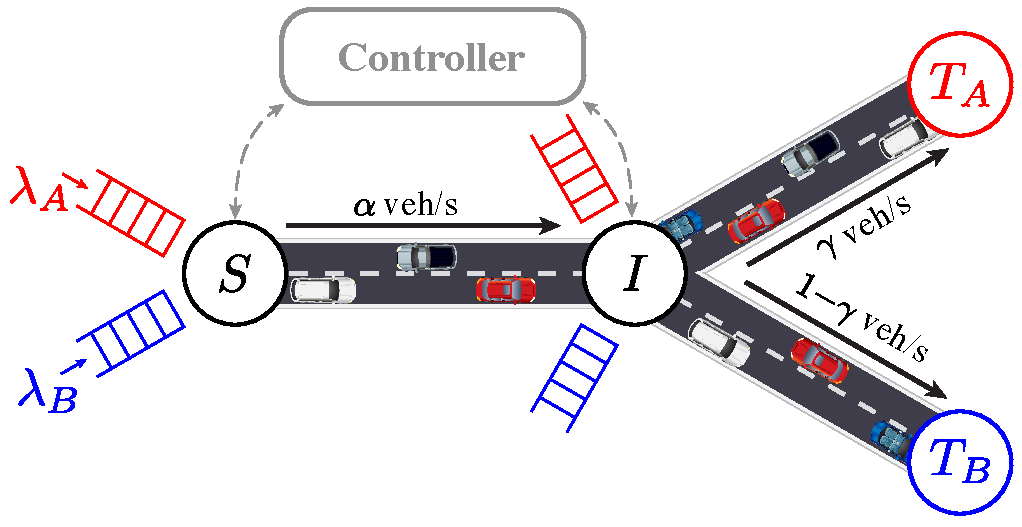
\includegraphics[width=\textwidth]{figures/simpleScenario.pdf}
        % }
        \caption{Two data transfers $A$ and $B$ originating from offloading spot $S$ share the road connecting offloading spot $I$. They then follow their own route toward their final destinations $T_A$ and $T_B$, respectively.}
        \label{fig:simple-scenario}
    \end{subfigure}%
    \quad %add desired spacing between images, e. g. ~, \quad, \qquad etc.
      %(or a blank line to force the subfigure onto a new line)
    \begin{subfigure}[t]{0.51\columnwidth}
        \centering
        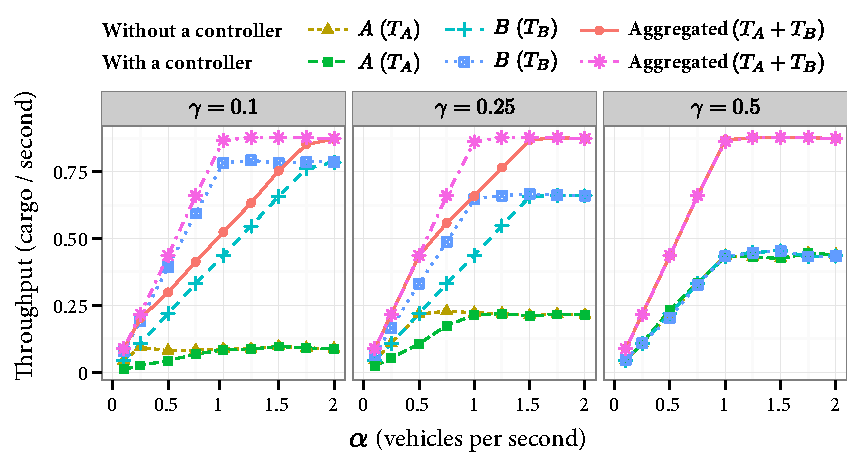
\includegraphics[width=\textwidth]{results/simpleScenario-throughput_v2_gamma_all.pdf}
        \caption{Maximum throughput (in number of data cargo received per second), for the two strategies with and without controller as a function of parameters $(\alpha,\,\gamma)$.}
        % (deduced from the AADT values)
        \label{fig:simple-scenario-throughput}
    \end{subfigure}
    \caption{Road network consisting in four offloading spots to show the benefits of having a controller.}
\end{figure}

We consider two scheduling strategies, without a controller and with a controller, to select the data transfer and to determine the amount of data to load on the vehicles stopping at each offloading spot. The first scheduling strategy (without a controller) selects the data cargo available at the offloading spots in a round-robin fashion. The data cargo of the transfers is selected in equal proportions and in circular order, without any priority given to the transfers. In the second strategy (with a controller), the decision to load a cargo on a vehicle is based on a pre-defined configuration of the offloading spots. The controller determines this configuration using the traffic volumes of road network under consideration. In the example of Figure~\ref{fig:simple-scenario}, if we assume the road traffic volume $I\rightarrow T_A$ to be three times greater than $I\rightarrow T_B$, the second strategy (with a controller) will load data three times more often onto vehicles heading to $T_A$. This is not the case of the strategy without a controller: this strategy will load the same amounts of data on stopping vehicles regardless of whether they head to $T_A$ or $T_B$.

We use \acrshort{sumo} (\acrlong{sumo}) to evaluate the three scheduling policies~\cite{behrisch2011sumo}. We simulate microscopic traffic in volumes of $\alpha$ vehicles per second from $S$ to $I$, $\gamma$ from $I$ to $T_A$, and $1 - \gamma$ from $I$ to $T_B$. We assume that both transfers $A$ and $B$ have infinite backlog of data at offloading spot $S$ (\ie $\lambda_A = \lambda_B = \infty$). Figure~\ref{fig:simple-scenario-throughput} shows the throughput of the system measured in the number of data cargo delivered to the destinations per second. In the scenario, the scheduling is relevant at $S$, as the road segments connecting the next-hop offloading spot $I$ to $T_A$ and $T_B$ exhibit different road traffic volumes. We consider an infinite backlog traffic generated at $S$ such that all vehicles leaving offloading spot $I$ are loaded with a cargo.

We can see that, for the first strategy without a controller, the transfer headed to $T_A$ needs a longer ramp-up period to reach its nominal throughput. Without any knowledge on the downstream traffic volumes, $S$ cannot load the optimal amounts of data to the next offloading spot $I$ to fully utilize the network resources. As a result, $I$ does not have enough data locally available to feed the higher flow of vehicles traveling towards $T_B$ compared to destination $T_A$. The resources available on the road segment $(I,\,B)$ remain underused when not enough data belonging to transfer $B$ are transported in an adequate amount to offloading spot $I$, \eg for $\alpha < 2$. On the contrary, the second strategy with controller allows $S$ to load data on vehicles traveling to $I$ in adequate amounts for both transfers. In turn, $I$ has enough data to efficiently utilize vehicles traveling on towards $T_A$ as well as $T_B$. The controller leverages the knowledge of traffic volumes on the downstream road segments to maximize the use of road resources at offloading spot $S$. This second strategy can achieve a better total throughput performance for all competing transfers at $I$. 

With this simple example, we showed the benefits of a centralized architecture that pre-configures the offloading spots to make the decisions to load data on vehicles. This architecture achieves better throughput compared to a distributed architecture decisions made locally at the offloading spots to load data on vehicles. In the following, we introduce a centralized architecture that controls a large-scale offloading infrastructure.

\clearpage
\section{Centralized controlled offloading architecture}
\label{sec:offloading-system-operations}

We exploit the logical centralization provided by \acrfull{sdn}\index{Software-Defined Networking (SDN)} to enable efficient control and management of the road network resources to offload bulk delay-tolerant traffic from a conventional data network. Following \acrshort{sdn}'s original design, our architecture consists of two components, as depicted in Figure~\ref{fig:architecture}: a central controller\index{controller} and the offloading spots acting as forwarding engines. We describe the function of each component in the remainder of this section. 

\begin{figure}[h]
	\centering
	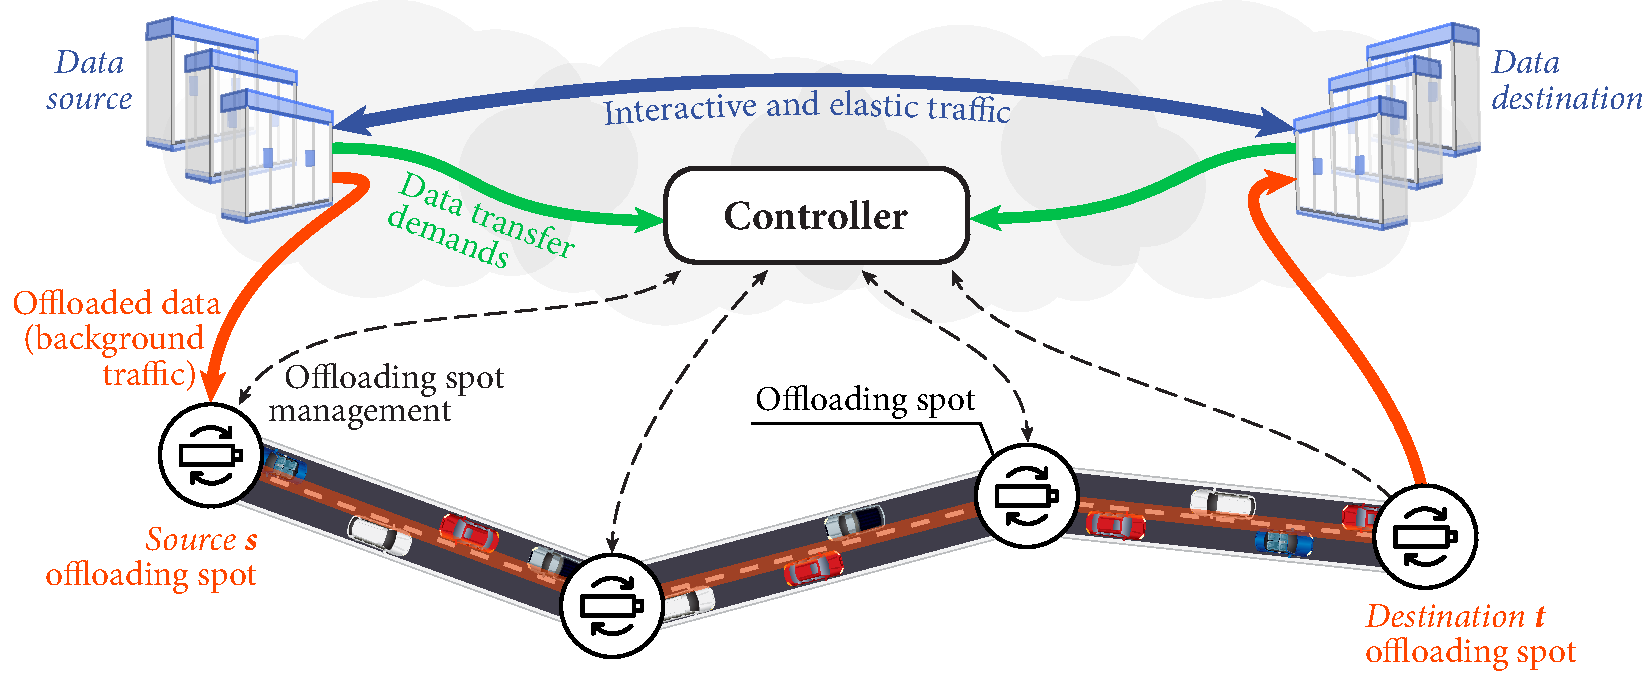
\includegraphics[width=0.85\columnwidth]{figures/architecture2.pdf}
	\caption{Centralized architecture to control the infrastructure in charge of offloading data.}
% 	In this scenario, the controller receives demands to offload bulk transfers of delay-tolerant data between two data centers. The controller configures the road network data plane by installing forwarding states at the offloading spots. The controller allocates the flows of vehicles on the roads connecting the offloading spots to carry the data towards its destination.}
	\label{fig:architecture}
\end{figure}




\subsection{Controller}

The controller\index{controller|bb} leverages the offloading overlay\index{offloading overlay} we presented in the previous chapter~\ref{sec:offloading-overlay}. As a result, the controller has a holistic view of the road network including its topology and dynamics, such as the traffic volumes for each road segment. Such knowledge may be derived from traffic forecasting services such as Navteq/Here\footnote{\url{https://www.here.com/business/traffic}},     
TomTom\footnote{\url{http://automotive.tomtom.com/en/connected-services/tomtom-traffic}}, or 
Airsage.\footnote{\url{http://www.airsage.com/Products/Traffic-Insights/}}. The controller keeps track of the status of the offloading spots via a long range control channel (\eg SigFox\footnote{\url{http://www.sigfox.com/}} or LoRa\footnote{\url{https://www.lora-alliance.org/}})~\cite{anteur2015ultra}. The information about the offloading spots includes the metadata of the data in transshipment and the statistics about the stopping vehicles, including the historical locations' made available via the navigation system of the vehicles. By collecting the information about the offloading spots, the controller has an up-to-date view of the offloading system. Recall that, in Section~\ref{sec:discuss}, we presented probabilistic tools to infer the remaining route of a vehicle knowing its navigation history, and the realization of the drayage system.

The controller receives demands\index{offloading demand} to offload data from transfers on the road network. Each demand specifies the delay and bandwidth requirements for the corresponding data transfer, as well as the origin and destination of the transfer. When receiving an offloading demand, the controller selects the road network paths by solving the vehicle flow allocation problem\index{vehicle flow allocation problem}. A road network path consists of a sequence of offloading spots followed by the data carried by vehicles between the offloading spots. In Section~\ref{sec:max-min-fairness-allocation-model}, we formulate the vehicle flow allocation problem as a \acrfull{lp} model that maximizes the throughput allocated in a fair manner to the flows of vehicles traveling between the consecutive offloading spots along the road network paths.

Figure~\ref{fig:controller-flowchart} shows the interactions between the functions of the controller with those of the offloading spots. The allocation procedure involves a reduction of the road network with the offloading overlay we detail in the next section. 

\begin{figure}[t]
	\centering
		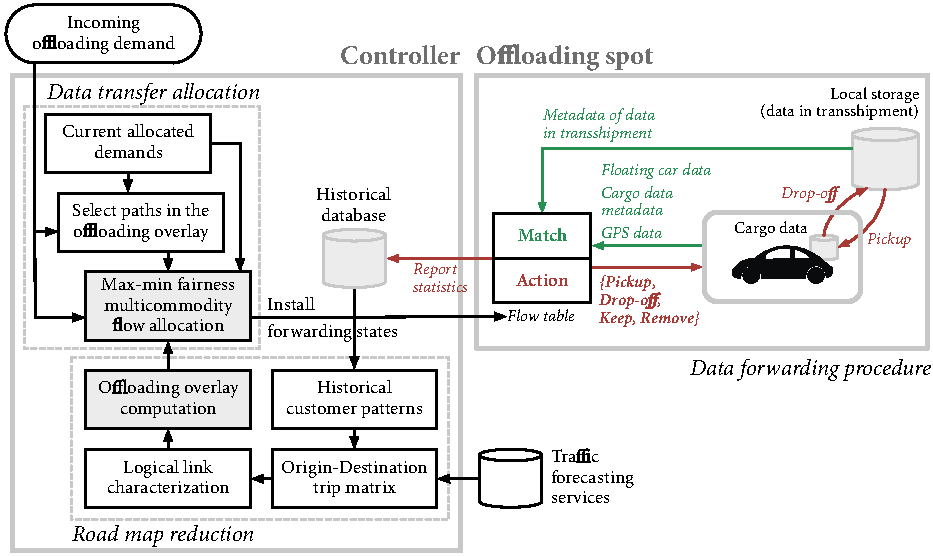
\includegraphics[width=\columnwidth]{figures/controller-flowchart-offloading-spot.pdf}
	\caption{Interactions between the functions of the controller and those of the offloading spots.}
	\label{fig:controller-flowchart}
\end{figure}


\subsection{Data forwarding at the offloading spots}
\label{sec:data-forwarding-offloading-spot}

We represent the interactions between the actions of the controller and the offloading spots in Figure~\ref{fig:controller-flowchart}. The controller installs forwarding states to control the local decisions made at the offloading spots to either drop off or pick up the data cargo. This decision results from the matching of the direction of the stopping vehicles against the destination of the available data. The local decisions account for the allocation of the road network resources shared among concurrent offloaded data transfers.

\clearpage

\begin{wrapfigure}[24]{o}[0.7\marginparwidth]{7.6cm}
    \includegraphics[width=7.5cm]{figures/forwarding.pdf}
    \caption{Forwarding process at an offloading spot.}
    \label{fig:forwarding-process}
\end{wrapfigure}
\paragraph{Flow tables.} 
The forwarding behavior of an offloading spot is determined by its \textit{flow table}\index{flow table|bb} represented in Figure~\ref{fig:controller-flowchart}. It consists of a list of entries, each installed for an individual offloading demands. The controller adds a new entry in the flow table of all the offloading spots on the road network path resulting from the allocation of a data transfer.
A flow entry contains the next-hop offloading spot to forward the data cargo along the allocated road path toward its destination.
% A flow entry forwards the data cargo to the next-hop offloading along the computed road path toward its destination.
% A flow table entry contains the next-hop offloading spot to which the data must be forwarded to reach the destination of the data transfer corresponding to this entry. 
The destination of the stopping vehicles is matched against the next-hop offloading spot of the flow entries. If there is a match, the offloading spot performs an action described by the forwarding process.
% on the cargo carried by the vehicle associated with the entry, including loading data on or off the vehicles.

\paragraph{Forwarding process.} 
The forwarding process is represented by the flowchart depicted in Figure~\ref{fig:forwarding-process}. Upon the arrival of a vehicle, an offloading spot checks if the direction of the vehicle matches one entry of its flow table. If none of the entries match, the vehicle unloads, if any, its data cargo onto the offloading spot storage for future pick-ups and continues its route without performing any further actions. If multiple entries match the direction of a vehicle, the offloading spot selects one entry based on the scheduling strategies presented in Section~\ref{sec:scheduling}. If the vehicle already carries data, the offloading spot checks if this data belongs to the data transfer represented by the matching entry. If this is the case, the vehicle keeps its cargo and continues its journey. Otherwise, the vehicle unloads its cargo at the offloading spots and becomes empty. For an empty vehicle, the oldest cargo associated with the selected entry is transferred to the vehicle.


\section{Max-min fair vehicle flow allocation model}
\label{sec:max-min-fairness-allocation-model}

In this section, we introduce the max-min fair allocation model\index{vehicle flow allocation problem!max-min fair allocation model|bb} solved by the controller in response to offloading demands. This model maximizes the throughput of the data flows allocated in a fair manner to the flows of vehicles traveling between the offloading spots. This model also integrates redundancy and retransmission mechanisms to completely recover from the effects of the logical link leakage. We then present the scheduling policies used by an offloading spot to serve concurrent data transfers. 

We consider the same assumptions regarding the offloading demands\index{offloading demand} as Section~\ref{sec:offloading-demands-feasibility} of the previous chapter. The demand is characterized by the amount of data $\beta_{st}$ and the deadline $\tau_{st}$ before which the transfer should be completed. However, here, we do not characterize the offloading demands with the leakage tolerance, since we target reliable transfers that do not tolerate any data losses. For simplicity, we model the rate of the demands at $s$ by a Poisson distribution $\lambda_{st}$ and its mean value is the average throughput $\beta_{st}/\tau_{st}$.

To improve the readability, we list the notations we use in the rest of this chapter in Table~\ref{tab:main-variables-haulage}. 

\begin{table}[ht]
    \caption{Table of notations for the max-min fair allocation model.}
    \renewcommand{\arraystretch}{1.1}
    \centering
    {\footnotesize
    \begin{tabular}{c|l}
        \textbf{Variable} & \textbf{Meaning}\tabularnewline
        \hline 
        $d_{st}$ & Offloading demand between source $s$ and destination $t$\tabularnewline
        $\tau_{st}$ & Deadline to transfer the data of offloading demand $d_{st}$\tabularnewline
        $\beta_{st}$ & Amount of data to transfer for offloading demand $d_{st}$\tabularnewline
        $\lambda_{st}$ & Poisson arrival rate at the source for offloading demand $d_{st}$\tabularnewline
        $\mathcal{P}_{st}$ & Set of simple paths between $s$ and $t$ on the offloading overlay\tabularnewline
        $\mathcal{S}$ & Storage capacity of the vehicles (cargo size)\tabularnewline
        $\mathcal{M}$ & Market penetration ratio\tabularnewline
        $c\left(i,\, j\right)$ & Capacity of logical link $\left(i,\, j\right)$\tabularnewline
        $t\left(i,\, j\right)$ & Travel time on logical link $\left(i,\, j\right)$\tabularnewline
        $l\left(i,\, j\right)$ & Leakage of logical link $\left(i,\, j\right)$\tabularnewline
        $l^{\textrm{\textbf{red}}}_{st}\left(i,\, j\right)$ & Leakage of logical link $\left(i,\, j\right)$ with redundancy for offloading demand $d_{st}$\tabularnewline
        $o^{\textrm{\textbf{red}}}_{st}$ & Weight of the \textbf{red}undancy mechanism on the data flow for offloading demand $d_{st}$\tabularnewline
        $R^{\{\textrm{hbh,e2e}\}}_{st}(i,\,j)$ & Average number of transmissions (either end-to-end (\textbf{e2e}) or hop-by-hop (\textbf{hbh}) \\
         & of a data cargo on logical link $(i,\,j)$ for offloading demand $d_{st}$\tabularnewline
        $\delta_{i}$ & Waiting time at offloading spot $i$ (to charge the EV's battery and load data)\tabularnewline
        $f\left(p\right)$ & Data flow on logical path $p$\tabularnewline
        $t\left(p\right)$ & Travel time of logical path $p$\tabularnewline
        $O_{st}(i,\,j)$ & Overhead of the offloading demand $d_{st}$ on the flow at logical link $(i,\,j)$\tabularnewline
        $R_{st}(i,\,j)$ & Number of transissions of a cargo belonging to demand $d_{st}$ on logical link $(i,\,j)$, \\
         & regardless of the retransmission mechanism\tabularnewline
    \end{tabular}}
    \label{tab:main-variables-haulage}
\end{table}

\subsection{Reliability overhead}
\label{sec:reliability}

In this section, we express the overhead in the throughput resulting from the two reliability mechanisms we consider. Firstly, we express the overhead for the redundancy mechanism in the case of RAID~6. Secondly, we express the overhead for the retransmission mechanism in the case of \acrfull{srarq}.

\subsubsection{\acrshort{raid} redundancy} 

Without loss of generality, we use \acrshort{raid}~6\index{reliability!RAID~6 redundancy} to partially recover from losses resulting from a vehicle failing to deliver its data cargo to the next offloading spot. \acrshort{raid}~6 divides the $\beta^{st}$ data of an offloading demand $d_{st}$ into $N$ arrays of $n\geq 4$ cargo. An array consists of two redundant cargo for $n-2$ cargo payloads. Therefore, a data transfer of $N$ RAID~6 arrays requires $nN$ vehicles, including $2N$ vehicles carrying redundant cargo to recover the losses in the $N(n-2)$ other vehicles.

\acrshort{raid} redundancy increases the amount of data sent by a factor $o_{st}^{\text{red}}$. For a data transfer involving exactly $n$ data cargo arranged in $N$ arrays, we express $o_{st}^{\text{red}}$ as follows:

\begin{equation}
	o_{st}^{\text{red}} = \frac{n}{n-2}\cdot
    \label{eq:redundancy}
\end{equation}

The data carried by $n$ vehicles whose storage devices are arranged in \acrshort{raid}~6 and travelling the logical link $(i,\,j)$ experiences a reduced data leakage denoted $l^{\text{red}}_{st}(i,\,j)$. We express $l^{\text{red}}_{st}(i,\,j)$ in terms of $l(i,\,j)$ (\ie the data leakage $(i,\,j)$ without data redundancy protection) as follows:

\begin{equation}
	l^{\text{red}}_{st}(i,\,j) = 1 - \sum_{k=0}^{2} \binom{n}{k} l(i,\,j)^{k}\big(1-l(i,\,j)\big)^{n-k}.
\end{equation}

\noindent Note that this expression assumes a data linkage equivalent to the failure likelihood of a storage device, which is consistent as both are independent and identically distributed. 

We explain how we determine $n$ (the number of storage devices per array) at the end of this section, as it depends on the total amount of transmitted data (including redundant data and the additional copies introduced by the retransmissions for recovering losses that \acrshort{raid} cannot repair). 

% We propose two retransmission strategies, as depicted in Figure~\ref{fig:global-architecture}: hop-by-hop (hbh) retransmissions and end-to-end (e2e) retransmissions. With the hop-by-hop strategy\index{Reliability!SR-ARQ Retransmission}, each offloading spot buffers data for later recovery in case a vehicle fails to deliver its cargo to the next-hop offloading spot. The controller receives acknowledgments over a feedback channel from the next-hop offloading spot (indicated by dashed arrows 2b-4b in Figure~\ref{fig:global-architecture}) and notifies through the same channel the previous offloading spot when to retransmit the missing data. With the end-to-end strategy (indicated by dashed arrows 1a and 4b in Figure~\ref{fig:global-architecture}), the only offloading spots in charge of recovering a loss are the edge offloading spots where the data is first transloaded from the computer network and stored until successfully transmitted. After a predefined number of attempts, a loss is repaired via the original data network (from where data was first transloaded) to make sure the deadline specified in the offloading demand can be met. Communication between the controller and the offloading spots incurs low bandwidth overhead and may be handled via a legacy data network (\eg the Internet). 

% \begin{wrapfigure}[27]{o}[0.7\marginparwidth]{7.6cm}
%     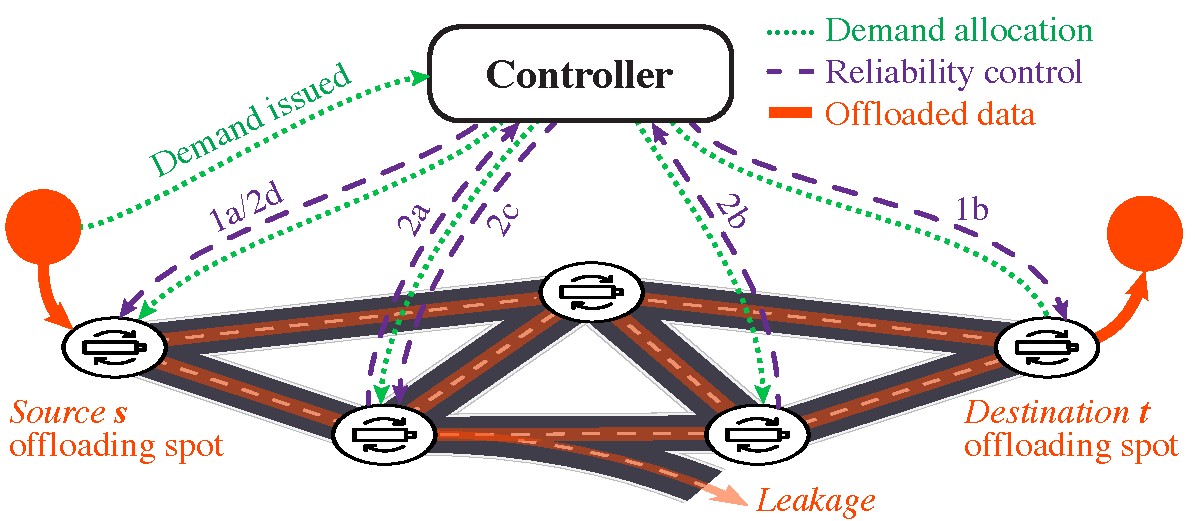
\includegraphics[width=7.5cm]{figures/architecture3.pdf}
%     \caption{A legacy data network (\eg access wired or wireless network) is used to transmit control messages between the offloading spots and the controller. The control channels allow the controller to access and change the forwarding behavior of the offloading spots (dotted arrows). Controller-to-offloading spot communication is also used for the end-to-end retransmission strategy (dashed arrows 1a, 4b) and the hop-by-hop retransmission strategy (dashed arrows 1a-3a and 2b-4b).}
%     \label{fig:architecture-retransmissions}
% \end{wrapfigure}

\begin{figure*}[!t]
    \centering
    \begin{subfigure}[b]{0.45\textwidth}
        \centering
        \includegraphics[height=5cm]{figures/retransmissions-sender.pdf}
        \caption{Sender-side (offloading spot $i$).}
        \label{fig:retransmissions-sender}
    \end{subfigure}%
    \qquad
    \begin{subfigure}[b]{0.45\textwidth}
        \centering
        \includegraphics[height=5cm]{figures/retransmissions-receiver.pdf}
        \caption{Receiver-side (offloading spot $j$).}
        \label{fig:retransmissions-receiver}
    \end{subfigure}%
    \caption{\acrshort{srarq} retransmissions. The red transitions is exclusively for the intermediate offloading spots in case of end-to-end retransmissions. The other transitions is for the source offloading spot in case of end-to-end retransmission and the source and the intermediate offloading spots in case of hop-by-hop retransmission.}
    \label{fig:retransmissions}
\end{figure*}

\subsubsection{\acrshort{srarq} retransmissions}

In addition to data redundancy, we use \acrfull{srarq}\index{reliability!SR-ARQ retransmissions} to fully recover the losses that \acrshort{raid} cannot recover~\cite{costello2004error}. We propose two retransmission strategies: hop-by-hop (hbh) retransmissions and end-to-end (e2e) retransmissions. In Figure~\ref{fig:retransmissions}, we represent the sender-side in Figure~\ref{fig:retransmissions-sender} and the receiver-side in Figure~\ref{fig:retransmissions-receiver}. The red transition in the sender-side refers to the behavior of the intermediate offloading spots in case of end-to-end retransmissions, while the other transitions refer to the behavior of the source offloading spot in case of end-to-end retransmission and all the offloading spots in case of hop-by-hop retransmissions. The controller enforces the retransmissions at the offloading spots using a low-bandwidth control channel\index{control channel}. Both retransmissions strategies rely on timeout expiration\index{reliability!SR-ARQ retransmissions!timeout} at the receiver-side to trigger a retransmission. The timeout corresponds to the travel time $t(i,j)+\varepsilon$ ($\varepsilon$ constant) between two offloading spots $i$ and $j$ and depends on the current road traffic. Note that, the controller can also leverage traffic forecasting services to re-evaluate the travel time using exponential weighted moving average techniques.

With the hop-by-hop strategy\index{reliability!SR-ARQ retransmissions!hop-by-hop}, the controller is informed of loaded vehicles leaving offloading spot $i$. A copy of the cargo is cached by $i$ until successfully transmitted to $j$, the next-hop offloading spot. If no acknowledgment is received from $j$ before the timeout expires, the controller notifies $i$ to retransmit the missing cargo.  The hop-by-hop strategy introduces an overhead corresponding to the average number of transmissions $R^{\textrm{hbh}}_{st}(i,\,j)$ needed to successfully deliver a cargo on logical link $(i,\,j)$. We express $R^{\textrm{hbh}}_{st}(i,\,j)$ as follows:
\begin{equation}
    R_{st}^{\textrm{hbh}}(i,\,j) =  \frac{1}{1-l_{st}^{\text{red}}(i,\,j)}\cdot
\end{equation}

With the end-to-end strategy\index{reliability!SR-ARQ retransmissions!end-to-end}, the only offloading spot in charge of recovering a data loss is the first one located at the source-side of the data transfer. Once the last offloading spot on the destination-side receives the data, it notifies the controller of the successful delivery. In turn, the controller notifies the first offloading spot on the source-side to delete the cached copy of the cargo. If the intermediate offloading spots do not receive the expected cargo before the timeout expires, they notify the controller, which in turn asks the source to send another copy of the cargo. The overhead of the end-to-end strategy corresponds to $R^{\textrm{e2e}}_{st}(i,\,j)$, the average number of transmissions of a cargo on logical link $(i,\,j)$ before successfully delivering it from $s$ to $t$. We express $R^{\textrm{e2e}}_{st}(i,\,j)$ as follows:
\begin{equation}
    R^{\textrm{e2e}}_{st}(i,\,j) = \frac{(-1)^{n-(i-1)}}{\prod_{j=i}^{n-1}\big(l_{st}^{\text{red}}(j_{i},\,j_{i+1})-1\big)}\cdot
\end{equation}

We denote $O_{st}(i,\,j)$ as the total overhead introduced by \acrshort{raid}~6 and \acrshort{srarq} on logical link $(i,\,j)$ to recover from vehicles failing to deliver the data sent with offloading demand $d_{st}$. We express $O_{st}(i,\,j)$ in terms of the overheads introduced by both the redundancy and retransmission mechanisms as follows:
\begin{equation}
    O_{st}(i,\,j) = \begin{dcases}
    o_{st}^{\text{red}} \times R_{st}^{\textrm{hbh}}(i,j) & \text{\!\!\small (hop-by-hop)}\\
    o_{st}^{\text{red}} \times R_{st}^{\textrm{e2e}}(i,j) & \text{\!\!\small (end-to-end)}
    \end{dcases}
\end{equation}
\noindent where $o_{st}^{\text{red}}$ is given by Equation~\ref{eq:redundancy}.

In the following, we will use $o^{\text{ret}}_{st}(i,\,j)$ to represent the overhead of the retransmission mechanism regardless of whether the mechanism is hop-by-hop or end-to-end. Similarly, we use $R_{st}(i,j)$ to represent the number of transmissions on logical link $(i,j)$ for cargo belonging to demand $d_{st}$, regardless of the retransmission mechanism.

\subsubsection{Determination of the array size $n$} 

\Acrshort{raid}~6 redundancy distributes the data across arrays of $n$ data cargo. The total number of data cargo $n$ is defined so that to minimize the data overhead $O_{st}$ needed to ensure reliable transfer in response to offloading demand $d_{st}$: 
\[
    \min O_{st}=\begin{dcases}
    \min_{n} \left\{ o_{st}^{\text{red}} \times \max_{(i,\,j)\in p}\{R_{st}^{\textrm{hbh}}(i,j)\} \right\} & \text{\!\!\small (hop-by-hop)}\\
    \min_{n} \left\{ o_{st}^{\text{red}} \times  \max_{(i,\,j)\in p}\{R_{st}^{\textrm{e2e}}(i,j)\} \right\} & \text{\!\!\small (end-to-end)}
    \end{dcases}
\]


\subsection{Max-min vehicle flow allocation model}
\label{sec:max-min-allocation-model}

The controller receives the demands to offload data transfers characterized by their performance requirements. The task of the controller consists in selecting the flows of vehicles according to the following constraints: (\textit{i}) the number of vehicles is sufficient to meet the transfer requirements and (\textit{ii}) the allocation of the combined storage of the vehicles is efficient and fair among the competing transfers. To this end, the controller starts by computing the logical paths in the offloading overlay for each of the transfer to offload. The controller then allocates flows of data on these paths while satisfying both constraints and finally configures then the offloading spots along the selected logical paths with a non-zero allocation.

In the following, $\mathcal{P}_{st}$ denotes the set of candidate logical paths between $s$ and $t$. Each logical path $p\in\mathcal{P}_{st}$ consists of a sequence of logical links connecting pairs of offloading spots in the offloading overlay. We express the path travel time\index{logical path!travel time} $t(p)$ experienced by a data transfer allocated to flows of vehicles traveling on logical path $p$ belonging to the set of logical paths $\mathcal{P}_{st}$ for offloading demand $d_{st}$. The path travel time is the sum of two components: travel time component and waiting component. The travel time component is the sum of the travel time of the logical link of $p$. The waiting component is the sum of the waiting times at each offloading spot connecting these logical links. We express $t(p)$ as a function of $R_{st}(i,j)$, the average number of transmissions of a cargo to successfully deliver it from $i$ to $j$ for demand $d_{st}$:
\begin{equation}
    \label{eq:impl-logical-path-travel-time}
	t\left(p\right) = \sum_{\substack{p\in \mathcal{P}_{st}\\(i,\, j)\in p}} R_{st}(i,\,j)\left[\delta_{i} + t(i,\,j)\right],
\end{equation}
\noindent where $\delta_i$ is the waiting time at offloading spot $i$.


\subsubsection{Linear programming formulation} 

We formulate the vehicle flow allocation procedure as a \acrfull{lp} model that determines the logical paths matching the performance requirements of the offloading demands. The \acrshort{lp} shown in Algorithm~\ref{fig:allocation} consists in allocating $f(p)$ data to the flows of vehicles traveling the logical paths of $\mathcal{P}_{st}$. We first present the inputs and then the allocation strategy for the offloading demands. The strategy relies on the multi-commodity flow allocation problem we formulate as a linear programming model. 

% \removelatexerror% Nullify \@latex@error
\begin{algorithm*}[H]
	\KwIn{Offloading demands $\mathcal{D} = \{d_{st}\}$, characterized by $\beta_{st}$ and $\tau_{st}$}
    \myinput{Set $\{\mathcal{P}_{st}\}_{st}$ of the logical paths between $s$ and $t$ for each demand in $\mathcal{D}$}
    \myinput{Average travel time $t(p)$ on logical path $p$}
    \myinput{Capacity $c(i,\,j)$ of logical link $(i,\,j)$}
    
    \KwOut{Resulting allocation $A=\{f(p)\}$ of flows to logical paths $p$}
    
    \BlankLine
    \Proc{\Alloc}{
        $L \gets \{\textrm{Logical links } (i,\,j)\}$\;
        $\{f(p)\} \gets \textsf{Max-Min Fairness(}\mathcal{D},\,L\textsf{)}$\;
        \Return{$\{f(p) : p\in \mathcal{P}_{st},\, (s,\,t)\in \mathcal{D}\}$}
    }
    
    \BlankLine
    \Func{\MaxMin{$\mathcal{D},\,L$}}{
    	\textit{Initialization:} $U\gets \mathcal{D};\;i\gets 0;\;A\gets\emptyset$\;
    	\While{$U\neq \emptyset$}{
    		\textit{Maximize the $i$-th smallest allocation:}\;
    		\Indp 
    	      $\phi_{i} \gets \MCF{$\mathcal{D},\,C,\,U,\,i,\,A$}$\;
    		\Indm
    		\textit{Perform non-blocking test:}\;
    		\Indp 
			  $A_{i} \gets \NBT{$U,\,A,\,\phi_{i}$}$\;
    		\Indm 
    		Fix the allocation of each demand in $A_{i}$ to $\phi_{i}$\;
    		$U\gets U\backslash A_{i}$\;
    		$i\gets i+1$\;
    	}
    	\Return{$\{f(p) : p\in A\}$}\;
    }
    
    \BlankLine
    \Func{\MCF{$D,\,C,\,U,\,i,\,A$}}{
        $\begin{array}{cc}
		\textrm{Maximize} & \phi_{i}\end{array}$\\
		$\begin{array}{ll}
		\textrm{Subject to:} & \\
		\sum_{p}f(p)\big(\tau_{st} - t(p)\big) \geq \beta_{st} & \forall(s,\,t)\in \mathcal{D}\\
		\phi_{i} - \sum_{p} f(p)\big(\tau_{st} - t(p)\big) \leq 0 & \forall(s,\,t)\in U\\
		\phi_{k} - \sum_{p} f(p)\big(\tau_{st} - t(p)\big) = 0 & \forall(s,\,t)\in A_{k}, \phi_{k} \textrm{ constant},\\
	    & k = 0,\,\dotsc,\,i-1\\
		\sum_{s,\,t} o^{\text{red}}_{st} \sum_{p} \big[ o^{\text{ret}}_{st}(i,\,j) f(p) \big] \leq c(i,\,j) & \forall(i,\, j)\in L,\\
		& p\textrm{ s.t. }(i,\,j)\in p\\
		\end{array}$\;
		\Return{$\{\phi_{i}\}\cup \{f(p) : p\in \mathcal{P}_{st},\, (s,\,t)\in \mathcal{D}\}$}\;
    }
    \caption{Computing the allocations with the max-min fair allocation model\index{vehicle flow allocation problem!max-min fair allocation model}.}
    \label{fig:allocation}

\end{algorithm*}

\paragraph{Inputs.} 
The model takes as input the set $\mathcal{D}$ of all demands to offload a data transfer on the road network. This set includes the previous demands already allocated in addition to the new demands.\footnote{We have to re-allocate the previous demands to guarantee fair allocation of these demands and the new ones.} The allocation procedure also takes as input $\mathcal{P}_{st}$, the set of candidate logical paths between each pair $s$ and $t$ for all demands in $\mathcal{D}$. To enumerate the logical paths in $\mathcal{P}_{st}$, we propose to use Yen's $k$-shortest paths algorithm~\cite{yen1971finding} or a breadth-first search algorithm~\cite{lee1961algorithm}. In our simulations, we reduce the search space by considering the logical paths sorted according to the travel time of a single cargo. The offloading overlay and the properties of each logical link (\ie capacity, travel time, and data leakage) are also inputs of the allocation procedure.

\paragraph{Model.} 
The controller allocates $f(p)$ flows to the logical paths listed in $\mathcal{P}_{st}$ according to the \textsf{Max-Min fairness}\index{max-min fairness model|bb} strategy. This strategy proceeds by successive iterations.  The first iteration allocates the minimum flows to satisfy the requirements of the demands (given by the first constraint in the \textsf{MCF} function). The next iterations successively allocate the remaining capacity of the network to the demands that can receive more flow. More specifically, iteration $i$ maximizes the minimal flow allocation noted $\phi_{i}$ and fixes the allocation for the demands that cannot be better served, \ie because of the capacity constraints of the paths or if the demand requirements are already satisfied. The next iterations process the remaining demands. To determine for which transfers the current allocation can be further increased in the following iterations, we use the non-blocking test algorithm presented shown in Algorithm~\ref{fig:NBT}. 


% \removelatexerror% Nullify \@latex@error
\begin{algorithm*}[h!]
	\KwIn{Set $U$ of demands allocated at step $i$}
	\myinput{Set $A$ of demands allocated at steps $k<i$}
	\myinput{Allocation $\phi_{i}$ of step $i$}
	\KwOut{Set $A_{i}$ of flows in $U$ that cannot be allocated more than $\phi_{i}$ in any solution}
    
    \BlankLine
    \Func{\NBT{$U,\,A,\,\phi_{i}$}}{
        \textit{Demands that have been satisfied are allocated:}\;
        \Indp 
            $D_{i} = \{(s,\,t) \textrm{ s.t. } \sum_{p}f(p)\big(\tau_{st} - t(p)\big) = \beta_{st} \}$\;
            $U \gets U \backslash D_{i}; \; A_{i} = D_{i}$ \;
        \Indm
        \textit{Demands allocated more than $\phi_{i}$ can be increased:}\;
        \Indp 
            $U_{i} \gets \{(s,\,t) \textrm{ s.t. } \sum_{p}f(p)\big(\tau_{st} - t(p)\big) > \phi_{i} \}$\;
        \Indm
        \textit{Test the allocation of the remaining demands:}\;
        \ForEach{demand $(s,\,t)\in U\backslash (A_{i}\cup U_{i})$}{
            $\begin{array}{@{}ll@{}}
            \textit{Solve the following linear program:} & \\
    		\textrm{Maximize} & \sum_{p\in\mathcal{P}_{st}} f(p)\\
    		\textrm{Subject to:} & \\
    		\sum_{p}f(p)\big(\tau_{st} - t(p)\big) \geq \beta_{st} & \forall(s,\,t)\in D\\
    		\phi_{k} - \sum_{p} f(p)\big(\tau_{st} - t(p)\big) = 0 & \forall(s,\,t)\in A_{k}, \phi_{k} \textrm{ constant}, \\
    	    & k = 0,\,\dotsc,\,i-1\\
    		\sum_{s,\,t} o^{\text{red}}_{st} \sum_{p} \big[ o^{\text{ret}}_{st}(i,\,j) f(p) \big] \leq c(i,\,j) & \forall(i,\, j)\in C,\\
    		& p\textrm{ s.t. }(i,\,j)\in p\\
    		\end{array}$\;
    		
            \lIf{$\sum_{p\in\mathcal{P}_{st}} f(p) \leq \phi_{i}$}{
                $A_{i} \gets A_{i}\cup \{(s,\,t)\}$\;
            }
            \lElse{$U_{i}\gets U_{i} \cup \{(s,\,t)\}$}\;
        }
        
        \Return{$A_{i}$}\;
    }
    
    \caption{Non-blocking test for the max-min fairness allocation model.}
    \label{fig:NBT}
\end{algorithm*}

The core of the max-min fairness algorithm is the \textsf{MCF} (\acrshort{mcf}) function shown in Figure~\ref{fig:allocation}. The \textsf{MCF} function computes the multi-commodity flow allocation\index{multi-commodity flow allocation} for the remaining demands. The first constraint matches the amount of data that can be offloaded within the deadline $\tau_{st}$ to the amount of data to transfer $\beta_{st}$. The following constraint ensures that the demands belonging to the sets $A_{k},\,k\in [0,\,i-1]$ are fixed to the allocation they received at previous step $k$. The objective of the \textsf{MCF} function is to maximize the minimum allocation $\phi_{i}$ such that all demands are satisfied. This objective is further guaranteed by the third constraint of the linear problem. Finally, the last constraint limits the total allocation of the paths crossing the logical links to the logical link capacity. Note that this constraint takes the overhead of the retransmission and the redundancy mechanisms into account. 

Once the allocation $\phi_i$ have been fixed by the \textsf{MCF} function for iteration $i$, the max-min fairness algorithm determines which demands can be further increased in their current allocation using the non-blocking test algorithm shown in Figure~\ref{fig:NBT}. The non-blocking test is derived from the algorithm proposed by Pi\'{o}ro \etal~\cite{pioro2003efficient}. This test compares the maximal throughput of the flows allocated by a multi-commodity flow allocation to the one resulting from the minimal flow allocation $\phi_{i}$. If the multi-commodity flow allocation improves the maximal amount of data allocated to a demand, the demand will be fixed in the next iterations of the max-min fairness algorithm. Otherwise, the demand cannot be better increased, and it is fixed to $\phi_{i}$. 

Note that the formulation of the multi-commodity flow remains valid for continuous flows (infinite backlog data traffic). In this case, we ignore the first constraint in the \textsf{MCF} function that satisfies the demand requirements.

The max-min fair allocation model presented in this section has a polynomial time-complexity because fractional flows are allowed in the linear programming models formulated in function \textsf{MCF} and the non-blocking algorithm~\cite{karakostas2008faster}. The time-complexity of both linear programming models grows in linear time with the number of demands and the number of paths in $\mathcal{P}_{st}$ for each demand $d_{st}$ of the set of demands to allocate. 

\subsection{Data scheduling} 
\label{sec:scheduling}

Recall from Section~\ref{sec:data-forwarding-offloading-spot} that offloading spots use flow tables to match the data locally available with the stopping vehicles and decide an action to take. Multiple entries in the flow table of an offloading spot $i$ may match the direction of a vehicle. Each entry corresponds to different data transfers or the same transfer spanning many paths in the road network. The offloading spot selects in which order the flow of vehicles should be allocated to the transfers according to the weighted fair queuing scheduling policy whose weights are configured by the controller, resulting from the allocation procedure output. We denote by $f(d_kp_l)$ the data flow on logical path $p_l$ allocated to the transfer resulting from offloading demand $d_k$. The controller assigns a weight $w(d_kp_l)$ to the transfers allocated to the logical paths in $P = \{d_kp_l | \forall d_k\in D,\, p_l\in \mathcal{P}^{d_k},\, (i,\,j) \in p_l\}$. $P$ is the set of logical paths passing by offloading spot $i$ and sharing the same next-hop offloading spot $j$. The controller computes $w(d_kp_l)$ by normalizing the rate of flow $f(d_kp_l)$ with the total rate of the flows traveling all paths in $P$:
\begin{equation}
    w(d_kp_l) = \frac{f(d_kp_l)}{\sum_{p\in P} f(p)}\cdot
\end{equation}

We use the weights in the scheduling algorithm to determine the priority of data transfers to assign the corresponding data cargo to a passing vehicle if multiple transfers traverse the same offloading spot. In our simulations, we considered a probabilistic weighted fair queuing scheduler, which uses the weights to pick a data transfer at random and assign the corresponding cargo to the stopping vehicle~\cite{shreedhar1996efficient}.


\section{Performance evaluation on the French road network}
\label{sec:throughput-max-model-eval}

In our evaluation, we use the same dataset\index{French road network} as the one we used in the previous chapter to conduct the evaluation of the throughput resulting from the cost-benefit maximization of offloading data (refer to Section~\ref{sec:res-revenue-max-model}).

We provide a characterization of the offloading overlay introduced in Section~\ref{sec:road-map-reduction-throughput} using more comprehensive road traffic modelling techniques compared to Section~\ref{sec:eval-offloading-overlay} to estimate the road traffic volumes between the offloading spots. Secondly, we evaluate the max-min fair allocation model we introduced in Section~\ref{sec:max-min-allocation-model} using the dataset of the French roads.

\subsection{Road map reduction} 
\label{sec:road-map-reduction-throughput}

\begin{wrapfigure}[13]{o}[0.7\marginparwidth]{8cm}
    \vspace{-15pt}
    \centering
    \includegraphics[width=7.5cm]{figures/France-overlay-haulage.pdf}
    \caption{Schematic representation of the demands $d_A$, $d_B$, and $d_C$.}
    \label{fig:france-demand-allocation-haulage}
\end{wrapfigure}
In the following, we characterize the logical links of the offloading overlay by expressing the road traffic volumes between adjacent offloading spots in terms of network quantities. These volumes are given by origin-destination matrices between the offloading spots. However, the datasets we use in our simulations only give the traffic counts in terms of \acrshort{aadt} (\ie the number of vehicles per unit of time for each road segment). We discuss the reasons why we use traffic counts in Section~\ref{sec:discuss-haulage}.

We use well-known traffic modelling techniques from transportation research to estimate the origin-destination matrix of the offloading spots from the traffic counts of the dataset\index{traffic modelling techniques}. We detail the traffic modelling techniques in the Appendix~\ref{cha:traffic-forecasting-techniques}. We proceed with the following three steps.

\begin{enumerate}

    \item \textit{Route determination.} The first step consists in selecting a subset of the alternative routes (to the shortest one) connecting each pair of adjacent offloading spots in the road network. The selection consists in choosing the $k$-shortest routes in terms of travel time. The routes are also selected such that they share a low degree of similarity in terms of stretches of road in common. We implement this selection process by using the algorithms proposed by Abraham \etal~\cite{abraham2013alternative}.

    \item \textit{Route assignment.} The second step consists in assigning weights to the selected routes using the C-logit route assignment model~\cite{cascetta1996modified}. The value of a weight is determined according to properties such as the travel time and the distance of the route. Those weights reflect the capacity of a route in attracting traffic, the higher the weight of a route the more traffic it will receive. The weights are then used in combination with the traffic counts to estimate the traffic volume of the routes selected in the first step between each pair of adjacent offloading spots. 
    
    \item \textit{Trip matrix estimation.} In the third step, we use the entropy maximization model proposed by Zuylen and Willumsen to compute the origin-destination trip matrix consisting in all pairs of offloading spots in the offloading overlay~\cite{van1980most}. This model determines the most likely distribution of the traffic across all the routes selected in Step~1 subjected to two constraints, namely the traffic counts of the routes' stretches of road and the C-logit weights. We feed this model with a dataset of the French roads we consider to infer the \acrshort{od} trip matrix between the adjacent offloading spots. 
    
\end{enumerate}

Finally, we determine the attributes of each logical link $(i,\,j)$ in the offloading overlay. These attributes are relevant to the allocation of the data transfers. The attributes are as follows:
\begin{itemize}

    \item \textit{Capacity $c(i,\,j)$.} The capacity of $(i,\,j)$ represents the combined storage of all vehicles travelling between $i$ and $j$. The capacity also reflects the market penetration ratio $\mathcal{M}$\index{market penetration ratio}, \ie the ratio of vehicles equipped with data storage devices.
    
    \item \textit{Travel time $t(i,\,j)$.} The travel time is computed as the travel time average for each route selected in the first step  between $i$ and $j$ and weighted by the route weights computed in the second step.
    
    \item \textit{Leakage $l(i,\,j)$.} The leakage represents the ratio of vehicles that fail to deliver the data they transport to the next offloading spot.
    
\end{itemize}

% We use the road traffic foresting techniques introduced in Section~\ref{sec:mapping-offloading-overlay} to estimate the road traffic on the logical links connecting pairs of offloading spots on the offloading overlay. We represent the resulting offloading overlay in Figure~\ref{fig:france-demand-allocation-haulage}. With this techniques, we have more realistic traffic flows between the offloading spots compared to the technique we used in Section~\ref{sec:res-revenue-max-model}.

% We connect neighboring charging stations via a set of disjoint alternative routes selected in the road map of France by running the algorithms proposed by Abraham \etal~\cite{abraham2013alternative} (refer to Section~\ref{sec:route-determination}). Selected routes share up to 80\% with the shortest route, while their length is at least 80\% of the shortest route. To estimate traffic volumes, we use the C-logit traffic assignment model~\cite{cascetta1996modified} (refer to Section~\ref{sec:route-assignment}). This model assigns a weight to the routes connecting the pairs of offloading spots less than 300~km away (\ie the driving range of an electric vehicle). We use the entropy maximization model\index{origin-destination trip matrix} proposed by Zuylen and Willumsen~\cite{van1980most} to infer the origin-destination traffic matrix consisting of all pairs of offloading spots (refer to Section~\ref{sec:trip-matrix-estimation}).


\subsection{Max-min fair allocation model on the roads of France} 

The objective of the simulation is to evaluate three metrics: (\textit{i}) maximum throughput of the resulting allocation to evaluate the capacity of the offloading infrastructure, (\textit{ii}) delay to transfer pre-defined amounts of data depending on the number of offloading spots involved in the data transfers and (\textit{iii}) fairness of the allocation of concurrent transfers when using logical paths with similar lengths.

We evaluate the performance of the transfers resulting from the allocation of three offloading demands using the max-min fair allocation model. The three demands are shown in Figure~\ref{fig:france-demand-allocation-haulage}: (\textit{i}) $d_A$ from Paris to Lyon with arrival rate $\lambda_A$, (\textit{ii}) $d_B$ from Paris to Bordeaux with arrival rate $\lambda_B$, and (\textit{iii}) $d_C$ from Paris to Marseille with arrival rate $\lambda_C$. Note that the road paths followed by the transfers resulting from demands $d_A$ and $d_C$ share the same logical links in the offloading network; as so $d_A$ and $d_C$ are competing over those links.  We use \acrshort{sumo} to run the simulations, which each lasts 300,000~seconds (3.5~days), including 43,200~seconds (12~hours) of \textit{warmup}, to give time for the first data cargo to reach their respective destination. In the rest of this section, we consider a conservative market penetration ratio $\mathcal{M}$ of 10\%\index{market penetration ratio}. Data leakage is assumed to be the same for all logical links in the offloading overlay. 

\subsubsection{Maximum throughput}

\begin{figure}[h!]
    \centering
    \includegraphics[width=0.65\textwidth]{results/plot-france-rate-throughput-m-10-wo-MCF.pdf}
    \caption{The maximum throughput achieved for offloading demands $d_A,\,d_B$ and $d_C$ (depicted in Figure~\ref{fig:france-demand-allocation-haulage}) as a function of the logical link data leakage (assumed to be the same on all the logical links).}
    \label{fig:french-net-throughput-leakage}
\end{figure}

We evaluate the maximum throughput achieved by each transfer $d_A$, $d_B$, and $d_C$ resulting from the \textsf{Max-Min fairness} strategy presented in Section~\ref{sec:max-min-allocation-model}. We also consider another strategy without a controller, which consists in selecting the data transfers in a round-robin order locally at each offloading spot. We consider an infinite backlog traffic generated at the single data source placed in Paris for each of the transfers (\ie $\lambda_A=\lambda_B=\lambda_C=\infty$). We evaluate the maximum throughput for each strategy and each retransmission mechanism (\textsf{hop-by-hop} or \textsf{end-to-end} introduced in Section~\ref{sec:reliability}). 

We plot the maximum throughput in Figure~\ref{fig:french-net-throughput-leakage} as a function of the data leakage for both the \textsf{hop-by-hop} and \textsf{end-to-end} retransmission mechanisms. The maximum throughput achieved for each of the transfers is expressed in terms of data cargo delivered per second.

Firstly, we examine the maximum throughput resulting from the strategy without a controller. We can see that this strategy does not guarantee a fair throughput distribution among the transfers resulting from the three demands. The maximum throughput for demand $d_C$ is lower compared to the ones achieved for demands $d_A$ and $d_B$. As depicted in Figure~\ref{fig:France-overlay-wo-capacity}, the data transfers resulting from demands $d_A$ and $d_C$ compete for the same resources, as they both follow road paths sharing common logical links. The strategy allocates the flow of vehicles traveling those links to the respective destinations of $d_A$ and $d_C$ without taking into account that destination of demand $d_C$ is farther away compared to demand $d_A$. Thus, the strategy favors $d_A$ at the expense of demand $d_C$. The data transfer resulting from demand $d_B$ is not affected by the unfairness of the strategy since the flow of vehicles allocated to $d_B$ travel separate logical paths compared to demands $d_A$ and $d_C$. We can also note that the resulting maximum throughput for demands $d_B$ and $d_A$ share the same values since destinations of both transfers are equally distant from their source.

Secondly, we examine the strategy with a controller. We can see that this strategy performs better than the strategy without a controller in terms of cumulative throughput. This result is the direct consequence of the design of the strategies. Recall from Section~\ref{sec:max-min-allocation-model} that the strategy with controller uses the \textsf{Max-Min fairness} allocation model that allocates data on vehicles to maximize the overall throughput of all transfers. The higher performance of the strategy with controller further confirms its need, as already discussed in Section~\ref{sec:need-for-controller}. 

The results also confirm that the strategy with controller guarantees a fair allocation among the transfers resulting from the three offloading demands. Indeed, by design, the strategy with controller uses the \textsf{Max-Min fairness} allocation model that maximizes the overall throughput of all transfers while achieving a fair allocation of the flows of vehicles among all data transfers.

Finally, we can see that the \textsf{hop-by-hop} retransmission mechanism gives better throughput compared to \textsf{end-to-end} retransmission mechanism. This results from the ACKs expected from the next offloading spot as the data transfer progresses along each logical path, which results in a faster error recovery with the \textsf{hop-by-hop} strategy compared to the \textsf{end-to-end} strategy. For cargo of 1~TB in size, the allocation resulting from the strategy with a controller gives a cumulative throughput of 114~Gbps when using the  \textsf{hop-by-hop} retransmission mechanism with a conservative 30\% data leakage, which amounts to 38~Gbps per transfer on average. 


\subsubsection{Number of offloading spots involved in the data transfers} 
\begin{figure}[t]
    \centering
    \includegraphics[width=\textwidth]{figures/France-overlay-allocation.pdf}
    \caption{Representation of the allocation of demands $d_A$, $d_B$, and $d_C$ resulting from the strategy with controller with different values for the maximal length of the candidate logical paths.}
    \label{fig:france-demand-allocation}
\end{figure}

In a second step, we examine the impact of the number of offloading spots on the duration needed to complete demands $d_A$, $d_B$, and $d_C$. We now consider that each demand is concerned with a transfer of 10~PB of data. The flows of vehicles are allocated to each demand according to the strategy with a controller. Data losses are recovered by using the \textsf{hop-by-hop} strategy given that all logical links share a data leakage of 30\%. The results are shown by the bar plot in   Figure~\ref{fig:hops-3-transfers-duration}. We measure the transfer duration for $d_A$, $d_B$, and $d_C$ as a function of the maximal length of the logical paths followed by each transfer expressed in terms number of offloading spots. We also measure the mean travel time of a cargo of size $\mathcal{S}=1$~TB. Our objective is to show the fairness of the strategy with a controller in the allocation of the transfers as a function of the degree of similarity of the paths they follow. We examine the results in Figure~\ref{fig:hops-3-transfers-duration} together with Figure~\ref{fig:france-demand-allocation} where we represent the logical paths allocated for each demand depending on the maximal length of the candidate paths. 

\begin{wrapfigure}[16]{o}[0.7\marginparwidth]{8.2cm}
    \includegraphics[width=8cm]{results/plot-france-3-transfers-duration.pdf}
    \caption{The duration needed to complete a 10~PB transfer (in lighter colors) and the travel time of a 1~TB data cargo (in darker colors) as a function of the candidate path maximal length in terms of hops.}
    \label{fig:hops-3-transfers-duration}
\end{wrapfigure}
We observe that none of the three destinations can be reached with a one-hop logical path. By increasing the logical path maximal length up to two hops, Lyon becomes the only city that can be reached, as shown in Figure~\ref{fig:france-demand-allocation}a. The high duration for $d_A$ is due to the low number of paths available and therefore of allocable vehicles, which results in a low throughput. If we consider logical paths of three hops or less, Bordeaux is now reachable in addition to Lyon. Figure~\ref{fig:france-demand-allocation}b shows that, in addition to the two-hop paths, there are more candidate paths between Paris and Lyon. As a result, more vehicles are allocated to $d_A$ which decreases its transfer duration. Regarding transfer $d_B$, the long transfer duration is explained by the few logical three-hop paths connecting Paris to Bordeaux in a similar way to $d_A$ and the logical paths of two-hop maximum length. With four-hop logical paths, Marseille is now also reachable, as shown in Figure~\ref{fig:france-demand-allocation}c. Nevertheless, the number of four-hop logical paths is still limited between Paris and Marseille, in a similar way as the two-hop paths to Lyon and the three-hop paths to Bordeaux. What is more, Marseille is located farther away from Paris compared to Lyon and $d_C$ competes for logical paths already passing by Lyon. This results in a longer transfer duration for $d_C$ but also in an increase of $d_A$ transfer duration.  At the same time, increasing the length of the candidate paths to four hops enables the allocation of more logical paths between Paris and Bordeaux, which results in a clear decrease in the transfer duration of $d_B$. This decrease is also explained by the low degree of similarity between the logical paths allocated to $d_B$ and those allocated to $d_A$ and $d_C$, as shown in Figure~\ref{fig:france-demand-allocation}c. Finally, with logical paths of five hops and more, the transfer durations are equivalent among all the demands. This further confirms that the strategy with controller guarantees a fair allocation in terms of throughput among all the demands. A slight increase in the transfer duration for all demands follows each increment in the number of hops as a direct consequence of the longer logical paths followed by all transfers. A similar trend can be observed for the travel time of the 1~TB cargo. 

\clearpage
\subsubsection{Cumulative capacity} 

We stress our system by allocating ten concurrent demands, all issued from Paris to the top nine other cities in France and one to Basel, Switzerland. This is shown in Figure~\ref{fig:10-demands-france}. We use the strategy with a controller to allocate the ten demands at the same time and consider again the \textsf{hop-by-hop} retransmission mechanism, given a 30\% data leakage for all logical links. We compute the cumulative throughput achieved by all ten transfers as a function of the length, expressed as the number of offloading spots of the logical paths allocated. We also compute the mean ratio of logical links shared by the logical paths allocated to each demand over the ones allocated to all other demands. The results are shown in Figure~\ref{fig:MMF-shared-throughput}. 

\begin{figure*}[!ht]
    \vspace{-15pt}
    \begin{subfigure}[b]{0.45\textwidth}
        \centering
        \includegraphics[width=\textwidth]{figures/France-overlay-transfers.pdf}
        \caption{Offloading demands to be allocated between Paris and the top ten other major cities of France, including Basel in Switzerland.}
        \label{fig:10-demands-france}
    \end{subfigure}%
    \qquad
    \begin{subfigure}[b]{0.45\textwidth}
        \centering
        \includegraphics[width=\textwidth]{results/plot-france-MMF-shared-throughput.pdf}
        \caption{Cumulative throughput of the allocated demands and mean ratio of shared logical links between the allocated logical paths.}
        \label{fig:MMF-shared-throughput}
    \end{subfigure}%
    \caption{Cumulative capacity with ten offloading demands spanning the French road network.}
\end{figure*}

As for the previous case regarding demands $d_A$, $d_B$, and $d_C$, all ten destinations can be reached from Paris through logical paths of length at least three hops. With at least three-hop long logical links, the cumulative throughput of all ten demands reaches 280~Gbps and remains the same with a low standard deviation among all demands. The only city reachable by one-hop long logical paths is Lille while Lyon and Lille are the only cities reachable with paths of at two hops or less. As shown in Figure~\ref{fig:10-demands-france}, Lille is the closest to Paris compared to all other nine cities and can be reached by logical paths which exhibit the lowest degree of similarity with the paths connecting Paris to the other cities. For this reason, the transfer to Lille achieves a higher throughput compared to all other transfers. For the destinations located at least three hops away from Paris, the cumulative throughput remains the same even after increasing the number of hops of the allocable logical paths. Extending the length of the acceptable paths should allow the allocation of a higher number of paths to each demand and thus increase the cumulative throughput. However, most of the newly added paths are too long to be allocated or are already used for other transfers toward closer cities. For this reason, considering more paths by relaxing the length limit brings no benefit in terms of throughput. Considering longer paths to be allocable results in increased durations to complete the transfers. This further confirms the observation we made for Figure~\ref{fig:hops-3-transfers-duration}, \ie the strategy with controller allocates the paths to achieve fairness among all competing transfers.

\section{Discussions}
\label{sec:discuss-haulage}

\subsection{On the choice of traffic counts}
\label{sec:choice-traffic-counts}

\paragraph{\acrfull{aadt}.}
The purpose of our performance evaluation is to assess the capacity enhancement brought to the Internet by the road network. Our evaluation aims at determining the amount of data that can be transferred on the road within a given time period. A typical transfer lasts from a few days to a week, as we can offload up to one Petabyte. The traffic counts we use are provided by the \acrshort{aadt} (\textit{\acrfull{aadt}})\index{AADT}, which are yearly averages. As so, \acrshortpl{aadt} average out the effects of seasonal and diurnal variations or missing data due to flawed monitoring. To determine the traffic volume of a road segment over the duration of a transfer, we multiply the corresponding \acrshort{aadt} by the transfer duration measured in days. The use of the \acrshortpl{aadt} prevents our evaluation results from being affected by the diurnal, seasonal, or flawed bias. 

To transpose our work in a practical setting or commercial use, thinner-grained traffic count averages should be used to account for transfers lasting few hours or several weeks. An established practice for inferring traffic count averages for different time periods consists in using temporal allocation factors applied to the annual \acrshortpl{aadt}. 

An example of temporal allocation factors can be found in ``The Traffic Monitoring Guide'' where they are referred to as \textit{group factors}. These factors are provided by the US \acrfull{fhwa} to help State Department of Transportation plan their local \acrfull{hpms}~\cite{wright1997variability,guide2013us}. The guide describes how to calculate the factor groups (\ie temporal allocation factors) from the traffic data collected. The procedure depends on the location and the characteristics of the road segment, as well as the time period of interest. The traffic assignment models presented in this paper remain pertinent and can be used in combination with the temporal allocation factors.

The factors resulting from this procedure are applicable for time periods of several months (seasonal), days (day-of-week), or hours. These factors determine the road traffic pattern as a ratio of the \acrshort{aadt} for given road segments. The hourly vehicle volume $V_{i,\,t}$ on a road segment $i$ at time $t$ is estimated as the product of the average daily traffic $\textrm{AADT}_{i}$ and monthly $M_{g(i),\,t}$, daily $D_{g(i),\,t}$ and hourly $H_{g(i),\,t}$ factors, each for the factor group $g(i)$ of the road segment $i$:
\begin{equation}
    \label{eq:traffic-variation}
    V_{i,\,t} = \textrm{AADT}_{i} \times M_{g(i),\,t} \times D_{g(i),\,t} \times H_{g(i),\,t}.
\end{equation}
Note that the hourly factor takes into account the $D$-factor and the $K$-factor (directional and peak hour factors, respectively).

\paragraph{Finer-grain traffic counts.}
Another way to carry out the study of a dynamic system with finer-grain traffic counts (\eg in the order of the hour or for 15-minute intervals) is to characterize the dynamic flows of vehicles between offloading spots. Numerous works from transportation research have studied the estimation and prediction of dynamic origin-destination matrices using traffic counts, in particular, Bierlaire and Crittin or Casetta \etal both propose to do so using sequential estimator (namely Generalized Least Squares)~\cite{bierlaire2004efficient,cascetta1993dynamic}. With dynamic \acrshort{od} flows between the offloading spots, one can use the recent work~\cite{fleischer2007quickest} that built on Ford and Fulkerson~\cite{ford2015flows} to study the allocation of flows over time using time-expanded graphs. 

\section{Conclusion}
\label{sec:throughput-max-model-conclusions}

In this chapter, we presented a centralized architecture that implements the concept of vehicular offloading. This architecture consists of a controller in charge of configuring the road path consisting in the sequence of offloading spots involved in a data transfer. To determine this road path, the controller solves a vehicle flow allocation problem formulated with a max-min fairness model. This model guarantees fair allocation among competing demands and efficient utilization of the vehicular resources. To solve the vehicle flow allocation problem, the controller computes a logical representation of the road network. The output of the allocation problem is translated to a set of forwarding rules installed at the offloading spots. Those rules indicate how much data should be loaded on the vehicles depending on their direction of travel. The controller also implements mechanisms combining retransmissions and redundancy to ensure reliable data transfers. We evaluated the fairness of the allocation procedure as well as the throughput of the data transfers offloaded on the roads of France. To calculate the capacity of the roads we used elaborated traffic modelling techniques detailed in the Appendix~\ref{cha:traffic-forecasting-techniques} which provide more realistic values. 
We showed that an \acrshort{sdn} architecture provides the necessary elements to enable data offloading over the road network. With its holistic view of the offloading infrastructure, the architecture allows the management of a country-wide network, while keeping a fine-grained control of the data movements and its interactions with the vehicles to offload several Petabyte of data per day. Compared to the assessment study presented in Chapter~\ref{cha:feasibility-study}, the results we presented in this chapter benefit from the use of traffic modelling techniques combined with the use of a max-min fairness allocation model.

\chapter{Towards vehicular cloud services}
\label{cha:vehicular-cloud-services}

% In this chapter, we present two extensions of the traffic offloading work we have introduced and detailed in the previous chapters. Conceptually, offloading spots can be seen as locations where the trajectories of vehicles can be combined into a logical path followed by the data. In the case of the offloading system, the offloading spots temporarily store the data, allowing to pass it asynchronously from one vehicle to another.

% Talk about the placement of offloading spots -> intractable to infer because of unknown origin-destination matrices. Arbitrary placement of the offloading spots to cover the populations and make trips with electric vehicles (\ie less than 150~km away from each other).

In this chapter, we extend the concept of offloading spots according to two distinct directions as a basis for vehicular cloud services. In the first section of this chapter, we exploit the storage capabilities of the offloading spots to design a distributed vehicular cloud-like system to store and share file generated by mobile users. While services like Dropbox\footnote{\url{http://dropbox.com}} and Google Drive\footnote{\url{http://drive.google.com}} have shown their great potential given their popularity, mobile users often face limitations (\eg high cost, low bandwidth, and limited coverage) when accessing such services through wireless networks including cellular 4G LTE or Wi-Fi. In our system, the offloading spots act as repositories where mobile users upload or retrieve files. To increase the likelihood of finding the requested files in a timely fashion, the repositories distribute the user files among the other repositories by using the existing movements of the users between the repositories.  

% The contribution of this work came into the form of a placement algorithm that determines the locations of a target number of repositories for a given user request deadline. The goals of the placement algorithm are twofold: (1) determine locations such that the allocated repositories serve the maximum number of user requests before they expire and (2) connect the repositories together by the movements of the mobile users to create the network used for file distribution. 


In the second section of this chapter, we dematerialize the offloading spots into pre-defined areas where vehicles come in contact frequently and long enough. We use these areas in the context of the virtualization of a large-scale vehicular network with shared vehicular resources (\eg compute, storage, and sensing) sliced into virtual machines. Virtual machines are allocated to multiple service providers, which leverage the movements of the vehicles and their shared resources to deploy large-scale geo-distributed applications (\eg sensing platforms). With these resources available, the services can benefit from a large collection of distributed mobile nodes to collect, process, and aggregate data to perform real-time analytics and make fast operational decisions~\cite{bonomi2012fog}. We investigate the capacity of the contacts in these pre-defined areas in the context of virtual machine migrations that happen as a result of changes in the physical topology or reallocations of the vehicular resources.

In each of these two extensions, we propose an optimized placement of the offloading spots with regard to the requirements of the services. To this end, we leveraged the concepts of the logical view\index{logical view} we introduced with the offloading overlay to represent the movements of the vehicles between the offloading spots. 

Our main contributions in this chapter are:
\begin{itemize}
    
    \item \textbf{Storage and sharing system} (Section~\ref{sec:vehicular-storage-sharing}). We consider a system that relies on a collection of repositories to store and share user files. We propose a placement of the repositories that exploits the movements of vehicles between the repositories to replicate files in the system.
    
    \item \textbf{Vehicle resource virtualization} (Section~\ref{sec:virtual-vehicular-network}). We virtualize the resources of the vehicles to create large-scale virtual vehicular networks. We propose a placement of geographical areas with the required vehicle density to accommodate transfers of virtual machine migrations via vehicle-to-vehicle communications.

\end{itemize}

In the following, we present our vehicular file storage and sharing system in Section~\ref{sec:vehicular-storage-sharing} and our vehicular network virtualization in Section~\ref{sec:virtual-vehicular-network}.

\section{Vehicular file storage and sharing system}
\label{sec:vehicular-storage-sharing}

In this section, we present the design of a cloud-like file storage and sharing system specifically targeting mobile users in urban environments. We use the storage capabilities of the offloading spots to turn them into repositories where users store and retrieve their files. %Content storage and retrieval was also an issue studied in the context of Delay-Tolerant Networking (DTN)~\cite{fall2003delay}. Examples include TierStore~\cite{demmer2008tierstore} which is a Network File System that relies on very low latency links that intermittently connect the repositories. This makes TierStore well suited in the context of DTNs. Ott and Pitk{\"a}nen~\cite{pitkanen2007redundancy,ott2007dtn} proposed a system based on repositories to cache user content, thus decreasing the latency when retrieving a content. However, both of these approaches. 
We study the impact of placement of the storage repositories such that it guarantees the availability and distribution of the files. We evaluate our placement strategy in the context of the public transportation system of buses operating in San Francisco. 

\subsection{Problem statement}

\begin{wrapfigure}[13]{o}[0.7\marginparwidth]{7.2cm}
    \centering
    \includegraphics[width=7cm]{figures/message-exchanged.pdf}
    \caption{Requests and data exchanges between a repository and two mobile users when they encounter one another.}
    \label{fig:request-exchange}
\end{wrapfigure}
The system deploys a collection of pre-positioned offloading spots acting as file repositories. They feature high availability, unlimited storage and fast wireless transmission capabilities to handle large data rates in parallel with multiple mobile users. We assume a central controller is in charge of monitoring the files available at each repository. Whenever a repository receives a new file from a user, it notifies the controller of the availability of this file. Likewise, the mobile users can be notified of the availability of the files through the controller. We assume that the communications between the controller and the repositories and mobile users are handled by an inexpensive control channel (\eg SigFox or LoRa)\index{control channel}.

Mobile users with unlimited storage capacity upload or retrieve files to the repositories they encounter as part of their movements. There are two types of user requests: \texttt{put} requests to store user files and \texttt{get} requests to retrieve them. All requests have an associated deadline. Once a mobile user generates a request, the request becomes pending for the user until they encounter a repository. When in the transmission range of the repository, the user seamlessly transfers all of its pending requests to the repository. We assume atomic contacts between the mobile users and the repositories, which allows to transfer an unlimited number of files.

\paragraph{\texttt{put} request.} 
When a mobile user generates a \texttt{put} request, the user waits to be in the transmission range of the first repository it encounters. On an encounter with a repository, the user transfers the \texttt{put} request message along with the file. Once the file is received, the repository updates its local storage and notifies the availability of the file to the central controller. We define the two behaviors of mobile users when they have a \texttt{put} request to execute:
\begin{itemize}

    \item ``First'' \texttt{put} policy: Mobile users immediately delete the request once they transferred it to the first repository they encounter or if its deadline expires, whichever occurs first.

    \item ``All'' \texttt{put} policy: Mobile users delete the request once the deadline associated with the request has expired. This allows the users to potentially replicate the files to all repositories they encounter from the moment the request is generated to the moment it expires.

\end{itemize}

\paragraph{\texttt{get} request.} 
Users share the files they store on the repositories with other users. That is, any user can generate a \texttt{get} request to retrieve any available file. The user then transmits the \texttt{get} request to repositories it meets until the request is satisfied or until its deadline expires, whichever occurs first. In turn, the repository processes the request and transfers the requested file to the mobile user if the file is available in the repository's local storage. Otherwise, the repository notifies the mobile user that the requested file is not available. The mobile user will then try to retrieve the requested file from the next repository it will encounter. If the mobile user does not encounter any repository with a copy of the requested file before the request's deadline expires, the request fails.

The system opportunistically uses the movements of the mobile users to transport the data between the repositories and distribute the files uploaded in the system. Increased file distribution will reduce \texttt{get} failure rates. To accomplish this, we introduce \texttt{sync} requests for the files that need distribution. Repositories generate \texttt{sync} requests once files are stored by their initial uploader, following \texttt{put} requests. A \texttt{sync} request results in transferring copies of a file from the repository to passing mobile users in charge of distributing these copies to repositories along their trajectories. A later encountered repository updates its local storage with the corresponding file and notifies the central controller of the new availability of the file. If the file is yet to be available in every repository, the new repository starts distribution the file it just received by generating corresponding \texttt{sync} requests. Otherwise, the central controller informs the repositories of the distribution completion. 

While replicating files to all the repositories is inefficient in terms of file storage, it fits with our assumption of atomic contacts and unlimited file storage at the users and at the repositories. We further assume no locality bias with respect to where files are generated. Additionally, we assume that we cannot predict the trajectory of the mobile users, in particular, we cannot predict the sequence of storage nodes the mobile users will visit in the future. Under these assumptions, replicating files to all the repositories is the most straightforward approach to increase the availability of files and improve the success ratio of \texttt{get} requests.

The three types of requests \texttt{put}, \texttt{get}, and \texttt{sync} are shown in Figure~\ref{fig:request-exchange}. In this figure, the mobile nodes are buses that aggregate requests from the passengers riding the bus. The first mobile user on the left carries three requests: \texttt{get} for file A, \texttt{sync} for file B, and \texttt{put} for file C. The repository, which only has a local copy of file A, executes all the requests and adds files B and C to its local storage. When a subsequent mobile user encounters the repository, the repository generates \texttt{sync} requests and transfers them to the mobile node, along with the copies of the files. The mobile node then carries the \texttt{sync} requests to the next repository it encounters.


We consider the following metrics to evaluate the performance of our system:
\begin{itemize}

    \item \textbf{Request success ratio.} We aim to maximize the successes and minimize the failures of user requests. A \texttt{put} or \texttt{get} request is successful if it completes before its deadline expires. The success ratio is the number of successful requests divided by the number of all requests issued during the time period of interest. 

    \item \textbf{File distribution duration.} File distribution relies on the movements of the mobile nodes to distribute copies of files across the repositories. The distribution duration of a file is the time it takes for it to be available in all the repositories of the system. The repository placement algorithm takes this metric into account when allocating the location of the repositories to minimize the distribution duration of the files.

\end{itemize}


\subsection{Repository placement}
\label{sec:repo-placement}

The goals of the placement algorithm are twofold: (\textit{i}) determine locations such that the allocated repositories serve the maximum number of user requests before they expire and (\textit{ii}) connect the repositories together by the mobile users' movements to create the file distribution network. The goals of the placement algorithm are represented in Figure~\ref{fig:placement-alg} in the case of a bus transportation system. The bottom layer shows the trajectories of the buses in the  
\begin{wrapfigure}[12]{o}[0.7\marginparwidth]{8.2cm}
    \vspace{-7pt}
    \centering
    \includegraphics[width=7.3cm]{figures/bus-distribution-system.pdf}
    \caption{Different layers to represent the goals of the placement algorithm for a bus transportation system.}
    \label{fig:placement-alg}
%\end{figure}
\end{wrapfigure}
Financial District of San Francisco, with allocated bus stops. Each bus trajectory is represented by a color and a width indicating the frequency of buses. The middle layer shows the discretized demands generated by the bus passengers. This layer shows the demands that are allocated to the repositories placed at the bus stops. Finally, the top layer shows a logical graph where nodes correspond to the allocated repositories and edges to the flows of buses running between two repositories. As in the bottom layer, the width of the edges corresponds to the frequencies of buses. 

We derive the placement of the repositories from a set cover problem, in particular, the Maximal Covering Location Problem~\cite{church1974maximal}. Given a set of candidate locations for the repositories, the placement problem consists in selecting the candidate locations that maximize the success ratio of the requests issued by the users. This problem was shown to be NP-Hard, so we adapt known heuristics to solve it~\cite{megiddo1983maximum}. To this end, we consider the Greedy Adding with Substitution (GAS) heuristic that determines the optimal locations for each iteration of the algorithm~\cite{church1974maximal}. 


\subsubsection{Candidate and demand locations}

The placement algorithm takes both a set $\mathcal{C}$ of candidate locations where the repositories can be placed, as well as a set $\mathcal{D}$ of demand locations to be served by the allocated repositories. The candidate and demands locations refer to geographical places (typically circles and square cells) visited by the user trajectories. The algorithm outputs a set $\mathcal{A}$ of allocated candidate locations for the repositories.

\paragraph{Demands.} 
Users can generate a request at any time. Each successive location visited by the trajectories of the users is a demand location with equal probability of being the starting location of a user request. To this end, we divide the geographical area into a grid of cells of a given size (\eg $100\,\textrm{m}\times 100\,\textrm{m}$). Each cell aggregates the discretized user trajectories that go through the cell. The greater the number of trajectory aggregates, the higher the probability for a cell to be the starting location of user requests.

\paragraph{Candidates.} 
Candidate locations for the repositories correspond to relevant locations the mobile users will often visit for long periods of time, allowing the transfer of significant amounts of data. For instance, candidate locations may be road intersections, or bus stops (\eg in the case of a bus transportation system). In the evaluation section, we use available data from bus transportation systems and consider bus stops as candidates for the location allocation of the repositories.

To determine the locations of the repositories, we quantify the relations between two locations $l_1$ and $l_2$ (either a demand or candidate location) by computing the following spatial statistics:

\begin{itemize}

    \item The mean visit frequency $f(l_1,\,l_2)$ of mobile users that visited location $l_1$, then location $l_2$.

    \item The median inter-visit duration $v(l_1,\,l_2)$ of two consecutive visits of mobile users at location $l_1$ that visited location $l_2$ later in during their trajectory.

    \item The median travel time $t(l_1,\,l_2)$ of the time it takes for a mobile user to travel from location $l_1$ to location $l_2$.

\end{itemize}

We then measure the weight $w(l_1,\,l_2)$ of a pair of locations $(l_1,\,l_2)$ using the visit frequency $f(l_1,\,l_2)$ and the median inter-visit duration $v(l_1,\,l_2)$ as follows:

\begin{equation}
w(l_1,\,l_2) = \frac{f(l_1,\,l_2)}{v(l_1,\,l_2)}\cdot
\end{equation}

In the following, we denote by $\{w_{l_1l_2}\}$  the \textit{weight matrix} such that $w_{l_1l_2} = w(l_1,\,l_2)$, and by $\{t_{l_1l_2}\}$ the \textit{travel time matrix} such that $t_{l_1l_2} = t(l_1,\,l_2)$.


\paragraph{Relations between demands and candidates.} 
The deadline of the user requests imposes a bound $\delta$ on the travel time $t(d,\,c)$ between a demand location $d$ and a candidate location $c$. A demand location $d$ is allocated to a candidate point $c$ if the demand is within the bound $\delta$ and the weight $w_{dc}$ is not null (\ie there are flows of mobile users that travel from the demand to each of the candidates). The goal is to maximize the sum of the weights of the demands $d\in\mathcal{D}$ allocated to a candidate $c$: $\sum_{d\in\mathcal{D}}\{w_{dc}\mid t_{dc} \leq \delta_{dc}\}$. Note that a single demand cell can be allocated to multiple candidates, each within the given bound $\delta$ with non-null weights. 

\paragraph{Relations between pairs of candidates.} 
We characterize the connectivity between two candidates in terms of flows of mobile users travelling from $c_1$ and $c_2$ with both weights $w_{c_1c_2}$ and $w_{c_2c_1}$. For each candidate, we maximize the sum of the weights between this candidate $c$ and the chosen candidates $k\in\mathcal{A}$: $\sum_{k\in\mathcal{A}}w_{kc} + w_{ck}$.


\subsubsection{Location allocation algorithm}

The algorithm derives from greedy-adding with substitution (GAS) heuristic proposed to solve the Maximal Covering Location problem~\cite{church1974maximal}. For each candidate location, we divide the iterations into two parts: selection and substitution. 

\paragraph{Selection.} We first pre-select the set of candidates from the set of remaining candidates such that each candidate is connected to the chosen repositories by the flows of mobile users. This pre-selection is necessary, as it guarantees the creation of the distribution network and increases the availability of files. From these pre-selected candidates, we choose the candidate that maximizes the sum of demand weights within the bound $\delta$ as we defined previously. 

\paragraph{Substitution.} The second part of the algorithm goes back on the previous iterations and examines each allocated candidate and tries to find a better candidate that maximizes the demand weights, while guaranteeing that the new candidate will be connected to the chosen candidates. If a better candidate is found, it replaces the candidate under examination. The substitution part allows to replace the candidates allocated in the early iterations that are not justified in the later iterations due to subsequent allocated candidates.

We adapt the GAS heuristic to our system as follows.  The first candidate is chosen such that it maximizes the sum of demand weights within the bound $\delta$. Note that, since the demand weights are maximized for this candidate, the candidate is often visited by mobile users, making it a good intermediary node to be connected to the other candidates by the flows of mobile users. There is no substitution part, as no other candidate was already chosen. In our implementation, once a candidate is chosen, we remove all the candidates in the vicinity of the chosen candidate (in terms of travel time and distance from the chosen candidate, \eg half the deadline and the distance corresponding to this duration with average speed). This allows us to better spread the repositories over the geographic area and avoids cluttering denser regions with too many repositories.

\subsection{Real experiment simulation}
\label{sec:repo-evaluation}

We run our evaluation in two parts. The first part corresponds to the allocation of a given number of repositories for the given deadline. The second part is the simulation of the system with the repositories placed in the area.

\begin{figure*}[t]
    \begin{subfigure}[b]{0.44\textwidth}
        \centering
        \includegraphics[width=0.9\linewidth]{figures/sf-muni-placement.pdf}
        \caption{Allocation of the repositories. The color variations of the demand and candidate locations represent hotspots resulting from the Getis Ord-G spatial analysis with respect to the bus visit frequencies at these locations~\cite{getis1992analysis}.\vspace*{1.3em}}
        \label{fig:sf-muni-placement}
    \end{subfigure}
    \quad
    \begin{subfigure}[b]{0.54\textwidth}
        \centering
        \includegraphics[width=\linewidth]{figures/origin-destination-matrix-1.pdf}
        \caption{Origin-destination matrix of the repositories (identified by the numbers represented on the Figure~\ref{fig:sf-muni-placement} showing the mean travel time in minutes between each pair of repositories. The values in parentheses are the corresponding standard deviation. The simulations were done for 15 repositories placed as shown in Figure~\ref{fig:sf-muni-placement}.}
        \label{fig:propagation-times-matrix}
    \end{subfigure}
    \caption{Results for the allocation of 15 repositories in San Francisco using the bus movements of the MUNI bus transportation system.}
\end{figure*}

\paragraph{Mobility model for public transit vehicles.} Firstly, we simulated the movements of the San Francisco MUNI buses\footnote{\url{https://www.sfmta.com/}} using the ONE simulator~\cite{keranen2009one}. The ONE simulator is a time-discrete and event-based simulator of delay-tolerant networks. We used the \texttt{MapRouteMovement} mobility model implemented in ONE to simulate the movements of mobile nodes and their stops on a street map. This mobility model is particularly well suited to simulate the movement of buses that are part of a transit system. We derive the movements of the buses from GTFS (\textit{General Transit Feed Specification})\footnote{\url{https://developers.google.com/transit/gtfs}} feeds given by the MUNI transit authority that gather the buses' schedules. We develop generic tools to convert the GTFS feeds into a collection of \texttt{MapRouteMovement} mobility models compatible with the ONE format.

\paragraph{Repository placement.} Secondly, we developed a framework to determine the locations of the repositories. The framework implements the algorithm described in Section~\ref{sec:sf-muni-placement}. It takes the bus movements we derived from the GTFS feeds. We divide the geographical area into a grid of cells of size 100m~$\times$~100m. We take bus stops as candidates to host a repository, since the buses stop for a long enough duration to transfer large amounts of data. The framework then allocates the locations of the target number of repositories among the candidate locations, given user request deadline. We represented in Figure~\ref{fig:sf-muni-placement} the output allocation of 15 repositories' locations out of the 4,590 bus stops in San Francisco using the movements of the MUNI buses. In this figure, we show a Getis Ord-G hotspot analysis of the spatially significant bus stop candidates with regards to the visit frequencies of the buses in their vicinity~\cite{getis1992analysis}.


%We simulate the bus movements of the San Francisco MUNI transit system.\footnote{\url{https://www.sfmta.com/}} 
After running our methodology to convert the GTFS feed, we obtained the movements of 493 buses running on 130 different trajectories, which represents the traffic of buses running between 10am and 4pm on a typical weekday. Both the mobile users and the repositories are equipped with WiFi network interfaces with a range of 250~m. We ignore wireless interference and assume enough wireless capacity to accommodate the full exchange of files between the repositories and the mobile users. The candidate locations are the bus stops given by the GTFS bus feed projected onto the street map. The wait time of the buses at the bus stops is picked at random between 10~seconds and 30~seconds. The mobile users send requests independently every 10~minutes following a Poisson distribution, without any assumptions on the popularity and geographical locality of the files. We assume the mobile users generate the \texttt{put} and \texttt{get} requests as follows: 10\% of the requests are \texttt{put} requests and 90\% of the requests are \texttt{get} requests. We assume the mobile users generate the \texttt{put} and \texttt{get} requests. The simulation duration is 20,000~seconds. For each simulation, we deploy a target number of repositories up until the optimal number of repositories, where no demands are left unallocated. 

\begin{figure}[t]
    \centering
    \includegraphics[width=0.8\linewidth]{figures/successRatio-fileAvailability.pdf}
    \caption{Comparison of the impact of the different \texttt{put} policies and the existence of the distribution network in the user request success ratio and the file availability in the repositories.}
    \label{fig:baseline1}
    % ggplot(r, aes(x=V3,colour=as.factor(V2), shape=as.factor(V2), linetype=as.factor(V2), y=V11)) + geom_line() + geom_point() + xlab("Number of repositories") + ylab("Success ratio of user requests") + scale_colour_manual(values=c("#f8766d","#00ba38","#619cff", "purple"), name="Deadline (s)")+ scale_linetype_discrete("Deadline (s)") + scale_shape_discrete("Deadline (s)") + facet_grid( ~ V1)
\end{figure}

\paragraph{Success ratio.} 
As a first step, we perform the simulations to evaluate the benefits of the \texttt{put} policies and the distribution network in the success ratio of the user requests. To this end, we simulate the system under different assumptions regarding the \texttt{put} policy (``first''  or ``all'') and the existence of the distribution network. We represent the average success ratio of the \texttt{get} user requests and the file availability in the repositories in Figure~\ref{fig:baseline1}. In the scenario with the ``first'' \texttt{put} policy and no distribution network, we notice that the more repositories there are, the more user requests are satisfied. Some buses that have pending \texttt{get} requests are not able to reach any repository because of their routes and the few repositories available. Adding more repositories allows more buses to reach repositories, resulting in better success ratio of the \texttt{get} user requests. However, since the data is scattered across multiple repositories, the success ratio of the \texttt{get} requests still remains low for short deadlines. For long deadlines, the buses visit more repositories, which increases their chances to visit one with a copy of the requested file. Taking advantage of the ``all'' \texttt{put} policy helps to increase the success ratio of the \texttt{get} requests by 9.98\% on average for all the deadlines. With this policy, the buses distribute copies of the files to different repositories, thus increasing the availability of the files. Contrary to the ``first'' \texttt{put} policy where user files are available at only one repository, the ``all'' \texttt{put} policy increases the chance of a mobile user to find a repository with a local copy of the requested file.

The distribution network led to increase the user request success ratio by 104.3\%. Note that this improvement is greater for lower user request deadlines (\eg the improvement for the user requests of 1200~seconds is of 201.4\% on average). The distribution network distributes copies of the files in several repositories. Since the repository placement algorithm guarantees that all the repositories are connected together, the files can be distributed to each repository of the system. Hence, a mobile user with a pending \texttt{get} request is more likely to encounter a repository that has a local copy of the requested file, which increases the success ratio of the \texttt{get} requests. Note that the use of the ``all'' \texttt{put} policy does not change anything in the request success ratio and file availability compared to the ``first'' \texttt{put} policy, as the mobile user that originated the request is also part of the distribution network.

\begin{wrapfigure}[14]{o}[0.7\marginparwidth]{8.2cm}
    \vspace{-15pt}
    \centering
    \includegraphics[width=8cm]{figures/propagationTimes.pdf}
    \caption{Distribution duration as a function of the file availability for different numbers of repositories. 
    %and a deadline of 2400~s.
    }
    \label{fig:propagationTimes}
    % ggplot(p, aes(x=V3,colour=as.factor(V1),shape=as.factor(V1), linetype=as.factor(V1),y=V4)) + geom_step() + xlab("Proportion of file availability") + ylab("Duration since put time")
%\end{figure}
\end{wrapfigure}
\paragraph{File availability.} 
We compare the benefits of the distribution network with the ``all''  \texttt{put} policy using the ``File availability'' plots in Figure~\ref{fig:baseline1}. The plots show the proportion of files available in the repositories, where ``1.0'' of file availability corresponds to all the files being available at each repository. We clearly see the benefits of the distribution network to distribute the files among the repositories. The ``all'' \texttt{put} policy also distributes the files to several repositories, however, it fails to distribute the files to repositories beyond those located on the routes of the mobile users that generated the \texttt{put} requests. The plot further shows that, even with the distribution network, the files are not available at every repository (only 85\% of them). In fact, the data represented accounts for the files that were not fully distributed by the end of the simulation. 

\paragraph{Distribution duration.} 
In the second step of our evaluations, we study the distribution duration of the copies of user files among the available repositories. In Figure~\ref{fig:propagationTimes}, we show the average duration to distribute a file throughout the distribution network since the time the file was stored in the first repository (following a \texttt{put} request). We represent the distribution duration of the copies of user files as a function of the proportion of the file availability for different numbers of repositories. For example, with 10 repositories, 40\% of file availability corresponds to the file being available in four repositories. The first repository where the file is stored can be any of the repositories available. We notice that the average time needed to distribute the user files to every repository, regardless of the number of repositories available, is 4000~seconds, or a little more than one hour. It takes more time to distribute the copies of the files to the repositories at the beginning and end of the file distribution. At the beginning of the file distribution, only one copy of the files is available in the first repository. It takes on average 700~seconds to distribute the first copy of the file to the second repository. As more repositories distribute copies of the files, the distribution of the copies becomes faster. By the end of the file distribution, copies of files are available in most repositories. It takes on average 500~seconds to reach the last repository, as it is the farthest away from the first repository where the original copy of the file was stored.

In Figure~\ref{fig:propagation-times-matrix}, we give an origin-destination matrix that shows the average travel time in minutes between any pair of repositories. This translates to the time needed to distribute the file to different repositories from the time the file was stored in a first repository. These values give the average duration for a file to be available at a repository, depending on the originated repository. In the figure, the repositories are identified by the same numbers as the ones in Figure~\ref{fig:sf-muni-placement}. The connectivity between two repositories depends on the number and frequency of the buses going from one repository to another. For instance, repositories 1 and 15 are very well connected to the rest of the repositories. However, repository 9 is not as well connected since it is farther away from the rest of the repositories. This further explains the longer time it takes to distribute copies of the user files from repository 9 to every other repository. This goes to show that the further away the repositories are, the more time it takes on average to reach them and distribute copies of the files to them. 

\clearpage
\section{Virtual machine migration in vehicular networks}
\label{sec:virtual-vehicular-network}

\begin{wrapfigure}[18]{o}[0.7\marginparwidth]{8.2cm}
\centering
\includegraphics[width=8cm]{figures/VMMigration.pdf}
\caption{Virtual machine migration between two vehicles in contact: \textbf{(1)} The controller receives a reallocation demand of the resources on vehicles A and B: VM 1 has to move from A to B. \textbf{(2)} The controller notifies the two vehicles to initiate the migration during their next contact. \textbf{(3)} When there is a contact, the VM is transferred from A to B.}
\label{fig:vm-migration}
\end{wrapfigure}
In this section, we dematerialize the offloading spots into areas where the vehicles often come in long contacts via \acrfull{v2v} communications\index{contact}. We use these areas in the context of large-scale mobile networks to address the problem of virtualizing the resources of vehicular nodes (\ie compute, storage, and sensing) to create a virtual vehicular network\index{virtual vehicular network}. The vehicular resources are managed by an infrastructure provider through a centralized controller and allocated to service providers who configure the virtual machines to deploy geo-distributed services (\eg large-scale sensing platform). In particular, as shown in Figure~\ref{fig:vm-migration}, we focus on the migration of virtual machines triggered by the re-allocations of virtual resources or changes in the physical topology. Instead of using cellular connectivity, we leverage vehicle-to-vehicle communications to migrate the virtual machines.

This contribution draws on the results presented for various cities including San Francisco and Warsaw where it was shown that vehicles come in contact often and for long period of time in specific areas~\cite{kang2004extracting,sarafijanovic2006island,uppoor2014generation,naboulsi2013instantaneous}. We present a generic methodology for analyzing contact opportunities in urban scenarios where mobility traces are available for various types of vehicles. By limiting the virtual machine migrations to these specific areas, the expected benefit is an improved ratio of successful migrations. We first present this methodology and then evaluate its benefits in the context of virtual machine migrations among the public buses of the city of Dublin, Ireland.


\subsection{Contact density heatmap generation} 

The methodology consists first in processing the mobility traces with the purpose of generating a heatmap representing graphically the spatial variation of the contact density. The next steps consist in determining the location of the hotspots matching specific values regarding the duration and the rate of the contacts occurring in those areas. The different steps of the methodology are depicted in Figure~\ref{fig:dublin-bus}.

\paragraph{Contact heatmap.}
The first step consists in computing the spatial variation of the contact density. The geographical area of interest is divided in a grid pattern where a square cell has a fixed size, \eg 100~m $\times$ 100~m. In each cell, the only contacts plotted on the heatmap are the relevant ones which in the VM migration scenario are the contacts lasting for at least 200~s. This duration amounts for the time needed to transfer a typical virtual machine of 200~MB. A kernel density estimator is then used to characterize the contact density of each cell. This consists in clustering the points representing the contacts occurring in the cell. Larger numbers of clustered points result in larger density values~\cite{silverman1986density}. The heatmap obtained for the city of Dublin is shown in Figure~\ref{fig:200-contacts} where different contact densities are depicted using different shades of red, the darker shade indicating a higher density of contacts. We notice that the contacts between buses are concentrated in the city center, but also on the outskirts of the city center, along the major traffic arteries and at some of the main intersections of Dublin. The next steps consist in deriving the hotspot locations from the contact density heatmap.

\paragraph{Contact hotspots.} 
Firstly, the cells are ranked according to their contact density. To exclude cells where contacts are not occurring in significant numbers, the 25\% top cells are selected. The contiguous cells are then aggregated in clusters referred to as \textit{hotspots}. Hotspots are represented on the map by circles centered so they can cover the corresponding cluster. The diameter of the hotspots is fixed and selected so the largest cluster is fully covered by a single hotspot.

The hotspots depicted in Figure~\ref{fig:200-contacts} 
are further characterized from the perspective of the \acrshort{v2v} migration of virtual machines. For each hotspot, the two following variables are computed: The total number of contacts with a duration of at least 200~s ($n$) and the average inter-contact duration ($x$). The inter-contact duration refers to the duration between two consecutive contacts occurring within the same hotspot. Those two variables are then used to assign a score to each hotspot we compute as: $\nicefrac{n}{\max(1,\,x)}$. Finally, we use the Jenks optimization method to identify three value ranges which provide the best arrangement of the hotspots according to their scores~\cite{jenks1963generalization}.

In Figure~\ref{fig:200-contacts}, different shades of color are used to represent the hotspots according to their classes. In the performance evaluation, two significant hotspots are selected, each belonging to the two higher classes: ``Hotspot 1'' has the highest score which indicates that long-duration contacts occur with high frequency. Note that three other hotspots share a similar score. The second hotspot indicated as ``hotspot 2'' is selected arbitrarily among the 16 occurrences sharing a similar score.

\begin{figure}[t!]
\centering
  \begin{subfigure}[t]{0.47\textwidth}
    \centering
    \includegraphics[width=\linewidth]{figures/dublin-all-contacts.pdf}
    \caption{Heatmap of the contacts of any duration in Dublin, Ireland.\vspace{1em}}
    \label{fig:all-contacts}
  \end{subfigure}%
 \qquad
  \begin{subfigure}[t]{.47\textwidth}
    \centering
    \includegraphics[width=\linewidth]{figures/dublin-200-contacts-res.pdf}
    \caption{Heatmap of contacts whose duration is greater than 200 seconds and the hotspots centered at location centered at the aggregated 25~\% densest cells.}
    \label{fig:200-contacts}
  \end{subfigure}
  \caption{Heatmaps of contacts between buses in Dublin, Ireland. The figures denote the number of contacts per cell (of size 100~m $\times$ 100~m). We choose to simulate migrations between buses entering the two hotspots circled on the map of Figure~\ref{fig:200-contacts}.}
  \label{fig:dublin-bus}
\end{figure}


\subsection{Experimentation with a bus system}

In this section, we assess the feasibility of migrating virtual machines in the context of the public transportation system of the city of Dublin.  In our simulations, we focus on the capacity of the opportunistic contacts between buses while in transit.

\paragraph{Experimental setup.} 
For our feasibility study, we use a publicly available dataset of real traces of Dublin city buses provided by Dublinked, part of the Dublin City Council. The mobility traces span the month of January 2013 and provide timestamped GPS coordinates of all DublinBus buses in service~\cite{dublinked}. We analyze the movements of 823 buses during the service day of Tuesday, January 29th, 2013 from 10am to 1pm. We assume that two buses are in contact whenever the buses are in each other's communication radius denoted $R$. We used a recent map-matching algorithm proposed by Newson and Krumm to match the sequence of timestamps positions with the planned route given in the GTFS feed provided by the Dublin City council~\cite{newson2009hidden}. This step allowed us to remove outliers from the simulation, which could bias the results, as well as form more realistic trajectories by adding timestamps waypoints corresponding to the respective routes followed by the buses.

We use the ONE, a discrete-event simulator to run our experiments~\cite{keranen2009one}. The ONE can use real-world mobility traces to reproduce the movements of DTN nodes using linear interpolation between two timestamped waypoints and infer their contacts. We used the default settings of the ONE to simulate IEEE~802.11 on the mobile nodes. However, the only layers supported by the ONE simulator are the network layers and above. To account for the properties of the physical layer including the link-level packet losses, we select appropriate values regarding the node communication radius and contact transfers goodput. We draw on the results presented by Rubinstein \etal which show a 1~Mbps plateau in the TCP goodput when the contact distance between vehicles is less than 150~m~\cite{rubinstein2009measuring}. The choice of a conservative node radius is further supported by Hadaller \etal who showed that the Packet Delivery Ratio (PDR) measured at the MAC layer remain stable between vehicles in contact within a similar distance of 150~m~\cite{hadaller2007vehicular}. In our simulations, we considered a conservative communication radius $R$ of 150~m with a homogeneous average goodput of 1~MB per second. 

\paragraph{VM migration simulations.}
In the remainder of this section, we simulate the migration of virtual machines of various sizes running on every bus. A bus entering a specific hotspot initiates the migration of a virtual machine with the first bus it comes in contact with, following the First Contact routing policy implemented by the ONE simulator. We make no assumption regarding the capacity of the buses to predict the duration of a contact. A transfer will be aborted in case the contact duration is not long enough to accommodate the transfer. Hence, multiple attempts may be needed before the migration succeeds. The migration is considered as failed if the bus exits the hotspot without succeeding in transferring the virtual machine.

The results we present reflect averages over 100~virtual machine migration trials for different sizes of virtual machines we try to migrate at each of the two hotspots introduced in Figure~\ref{fig:200-contacts}. The range of values we use captures the usual sizes of virtual machines that can be found, that is, from a few hundreds of kilobytes (\eg TinyOS~\cite{levis2005tinyos}) to a few hundreds of Megabytes~\cite{clark2005live}. For each size of virtual machine, we measure the average time needed for a bus entering each hotspot to find a suitable contact and the time it actually takes to migrate the virtual machine. The plot in Figure~\ref{fig:graph} shows the mean time to transfer virtual machines of different sizes, as well as the proportion of virtual machines that were actually transferred. 

\begin{figure}[t]
  \centering
  \includegraphics[width=0.98\linewidth]{figures/duration-ratio-migrations.pdf}
  \caption{Proportion of successful virtual machine migrations and mean time to transfer the virtual machine as a function of the virtual machine size. The black solid bars represent the 95\% confidence interval for the waiting time before successfully transferring the virtual machines.}
  \label{fig:graph}
\end{figure} 

\begin{wrapfigure}[12]{o}[0.7\marginparwidth]{8.2cm}
    \vspace{-10pt}
    \centering
    \includegraphics[width=8cm]{figures/contact-durations-histogram.pdf}
    \caption{Number of contacts (in log scale) accounted for different duration ranges and their ratios (in percentage) against the total number of contacts in the hotspots 1 and 2, respectively.}
    \label{fig:plot-contact-duration-ratio}
%\end{figure}
\end{wrapfigure}
First, we note that the ratio of virtual machines successfully migrated at both hotspots decreases as their size increases. This is due to the lack of enough long-lasting contacts between buses. Buses fail several times before finding a suitable contact to transfer the virtual machine. This observation is confirmed by the time spent waiting for a contact suitable in duration with large-sized virtual machines. Overall, it takes less time to find a suitable contact at hotspot~1 than at hotspot~2. Buses entering hotspot~1 spend less time waiting for a suitable contact in comparison with hotspot~2 expect for virtual machine sizes ranging from 200 to 400~MB. To further explain this trend, we plot in~Figure~\ref{fig:plot-contact-duration-ratio} the total number of contacts measured for different contact durations as well as the ratios of those contacts against the total number of contacts occurring in  hotspots~1 and~2. We can see that hotspot~2 has a higher ratio of contacts lasting long enough (\eg 200~s and 400~s) to accommodate transfers of virtual machines with a size ranging from 200~MB to 400~MB. Despite the higher number of contacts at hotspot~1, most of them are not suitable for the transfers of such virtual machines. Buses spent more time trying transfers that will eventually fail before finding a suitable contact. This also explains why the ratio of successful migrations is higher at hotspot~2 when virtual machines have sizes ranging from 200 to 400~MB.


\section{Discussions}

\paragraph{Atomic contacts (first extension).}
The stronger assumption we made is to consider contacts between mobile users and repositories with unlimited capacity. If we want to relax this assumption, an increasing number of requests would not be satisfied with the simulation time. We need to consider the following enablers. Firstly, with equal file size and control messages with negligible size, we have to adapt the placement algorithm to take the contact duration of buses at each candidate repository. In particular, we need to differentiate the (longer) contacts of buses with repositories located in bus stops where the buses will actually stop at, and the (shorter) contacts between buses and repositories located in bus stops where the bus does not stop at. Secondly, we need to prioritize the requests to transfer between the repository and the bus. As an example, the \texttt{put} requests must be transmitted to the repository before any other request. Similarly, if the repository can satisfy the \texttt{get} requests carried by the bus, the corresponding files must be transmitted before the files associated with the \texttt{sync} requests of the bus and the repository. Finally, we note the different priorities impacts the replication of the data across the repositories. As a result, we need to develop new strategies to decrease the number of copies to replicate. 

\begin{wrapfigure}[14]{o}[0.7\marginparwidth]{6.7cm}
    \vspace{-15pt}
    \centering
    \includegraphics[width=6.5cm]{figures/allput-backend.pdf}
    \caption{Average number of copies distributed and received by the repositories for a file and a user request deadline of 2400~seconds.}
    \label{fig:allput-backend}
%\end{figure}
\end{wrapfigure}
\paragraph{Replication strategies (first extension).}
With the replication of file copies to every repository, a large number of copies is distributed and received by the repositories, as we show in Figure~\ref{fig:allput-backend}. With non-atomic contacts, we need to limit the overhead of copies sent over contacts between mobile users and repositories. With no knowledge of the future trajectories of mobile users, one could distribute copies of files for a bounded duration until the distribution of copies of the file stops. Alternatively, one could bound the number of copies generated per repository and transmitted to the mobiles users. With techniques borrowed from Delay Tolerant Networks, one could use a control plane that would enable the repositories to ``learn'' the frequent repositories the mobile users encounter along their route~\cite{lindgren2003probabilistic,grossglauser2006locating}. With this information, a single copy would be needed to transmit per repository. 

\paragraph{Virtual machine allocation (second extension).}
Recall that we considered a set of virtual machines managed by an infrastructure provider who allocates them to service providers who deploy their services. However, we did not detail the algorithm to allocate the virtual machines to the service providers such that the allocation result satisfies their requirements. As an example, the requirements may relate to the number of virtual machines to allocate, a target guaranteed connectivity of virtual machines through vehicle-to-vehicle connectivity, or the geographic areas covered by the virtual machines. The output of the allocation algorithm must minimize the number of migrations and where they happen in order to minimize the duration of the transition. Additionally, the service providers may issue new demands to the infrastructure provider or change their current demands. To this end, the latter must determine whether the demands can be satisfied before serving them. An approach to achieve this is to check the current state of the available and allocated resources through the control channel before allocating new resources. If the demand can be allocated or modified, the infrastructure provider re-runs an allocation algorithm that triggers new slicing of the resources of the nodes, as well as virtual machine migration between the mobile nodes.

\paragraph{Finding suitable contacts (second extension).} In order to successfully transfer a virtual machine between two vehicles, the contact must be long enough to accommodate the size of the virtual machine. In our evaluation, we proposed a methodology to determine the geographical areas we refer to as hotspots where long-duration contacts occur at significant rates. Hotspots are located in geographical areas within which all contacts amount for 75\% of all 200~second long contacts and occur at most every 1000~seconds. However, although long-duration contacts occur statistically more often in the hotspots compared to other areas, there is still a high density of short-duration contacts (as shown in Figure~\ref{fig:200-contacts}). Depending on the first contact a bus has when entering a hotspot, the VM migration may fail if the first contact is not long enough to accommodate the target virtual machine size. One way of improving the migration success is tu use models to predict contact durations between buses. Many existing techniques may be borrowed from the DTN literature. For instance, this could be done by maintaining a list of contact with their corresponding durations for each vehicle encountered~\cite{lindgren2003probabilistic,grossglauser2006locating} or by exchanging the direction and speed or itinerary between vehicles in contact to estimate the shared route with the other vehicle~\cite{cheng2010geodtn,banerjee2007energy}.

\section{Conclusion}

In this chapter, we proposed to extend the concept of offloading spots into two distinct directions in the context of different vehicular cloud services. In both extensions, we relied on a logical map to characterize the movements of the vehicles within the offloading spots or between them. We then used this logical map to determine the placement of the offloading spot to optimize the resulting compositions of the movements of the vehicles according to the service requirements.

In the first extension, we proposed a placement of offloading spots that act as repositories that are part of a distributed cloud-like storage and sharing system. The placement aims to satisfy a maximum of user requests to store or retrieve files and distribute the files throughout the repository network using the movements of the mobile users between the repositories. We showed the benefits of using the movements of vehicles to distribute files and thus improve the success ratio of the user requests.

In the second extension, we dematerialized offloading spots into pre-defined areas where vehicle often meet long enough to transfer large amounts of data. We used these areas in the context of a virtualization of the resources of the vehicles to migrate virtual machines following topology changes. We proposed a placement of these areas such that the vehicles can accommodate large data transfers of the size of a virtual machine. With simulations of real-world bus traces, we showed that these areas increase the success of the transfers as the vehicles are more likely to come in contact with other vehicles for long durations. As a result, transfers of several hundreds of Megabytes can be achieved through \acrshort{v2v} communications, enough to accommodate migrations of virtual machines.

These extensions showed that the existing mobility of vehicles has the potential to provide innovative added-value services for urban environments, with limited reliance on conventional data networks.
\chapter{Conclusion and perspectives}
\label{cha:conclusion}

\section{Summary of contributions and takeaways}

The work presented in this thesis exploits the existing mobility of everyday entities, including private vehicles and bus transportation systems to overcome the limitations of conventional data networks. We used the mobility in the context of various applications, including traffic offloading and cloud-based services. 

\paragraph{Massive data offloading.} 
We equipped vehicles with storage capacities connecting specific locations we referred to as offloading spots. The offloading spots avoid relying on the vehicles that make a direct trip from the source to the destination of the data transfer. The offloading spots help maximize the utilization of the combined storage of vehicles traveling the road segments connecting the offloading spots. To this end, they act as data relays where the trajectories of the vehicles making stops are composed into a single path followed by the data they carry.  
% The data then follows the path consisting of a sequence of offloading spots where the trajectories of independent vehicles are composed. 
In the following, we detail how we used the offloading spots to control and manage the composition of the movements of the vehicles to match the requirements of the data transfers.

\paragraph{Control and management of the offloading infrastructure.}
Offloading spots are also equipped with storage where data is buffered and asynchronously passed from one vehicle to another. The offloading spots are located where vehicles stop long enough to transfer large amounts of data. Examples of such locations include parking lots, shopping centers, and gas stations. We proposed an \acrshort{sdn} architecture with a centralized controller that has a holistic representation of the offloading infrastructure. The controller manages the resources of the offloading system using a logical representation of the dynamics of the road network. This representation is called the offloading overlay and results from a mapping algorithm that translates the movements of vehicles in terms of network quantities. The offloading overlay consists of logical links, each characterized by its capacity, delay, and loss rate. The controller leverages the offloading overlay to solve the vehicle flow allocation problem, which consists in selecting and allocating data to the vehicle flows connecting the offloading spots. The resolution of the allocation problem maximizes the utilization of the road resources. The output of the allocation is translated into a set of rules the controller uses to configure the offloading spots. These rules indicate which vehicles an offloading spot should select and which data to load onto the vehicles. Our results on the main roads of France with real traffic counts showed that the centrally controlled architecture can achieve an efficient and fair allocation of concurrent data transfers between major cities in France.

\paragraph{Vehicular storage and sharing system.}
We exploited the storage of the offloading spots to turn them into repositories where mobile users can store and retrieve files. The system relies on a collection of repositories and the movements of the vehicles between them to distribute the files among the repositories. We proposed a placement algorithm to determine the optimal locations of the repositories so each repository can satisfy the user requests to store or retrieve a file. The placement of the repositories also considers the movements of the vehicles connecting each pair of repositories so the files uploaded to the system can be synchronized without relying on the existence of a data network. We showed that the distribution of files using the existing mobility of the vehicles helps increase the success rate of user requests.

\paragraph{Virtual vehicular network.}
We dematerialized the offloading spots in the context of a vehicular network where the vehicle resources, including storage, but also processing or sensing are virtualized with virtual machines. We studied the virtual machine migration through vehicle-to-vehicle communications. In this context, the offloading spots are areas where vehicles come in contact often and for long periods compared to other areas. We showed that restricting the virtual machine migrations to these areas improves the success rate of the migrations.

\paragraph{Main challenges.}
During this thesis, I had to find data sources through people I contacted in different institutions and companies. While most of these attempts were unsuccessful, I managed to find relevant local data following recent open-data initiatives, as an increasing number of institutions provide publicly available data. Once I obtained the data, I had to find ways to analyze it in order to characterize it into network quantities. Unfortunately, most of the open-source traffic simulators (SUMO~\cite{behrisch2011sumo} or MatSim\footnote{\url{http://www.matsim.org/}}) were unsuited for the analysis of the road networks. I had to develop my own set of tools to perform the analysis and characterization of the networks necessary for the evaluations. Finally, I had to study and understand the relevant body of work borrowed from transportation research to infer flows of vehicles from traffic counts and characterize them into network quantities.

To summarize, the key takeaways from this thesis are:
\begin{itemize}

    \item The vehicles in circulation are an untapped potential for data transportation. We illustrated this assertion with simulations of vehicles transporting data on French roads and showed that the road network has the potential to daily offload several Petabytes of data.
    
    \item A dedicated infrastructure increases the overall capacity of the system by composing the trajectories of the vehicles and configuring the path followed by the data.

    \item A centralized control of the infrastructure with a holistic representation of the vehicle flows enables efficient management and allocation of the road resources to data transfers.
    
    \item A logical representation of the vehicular resources into network quantities mitigates the scale of the road network and makes the data transfer allocation tractable. 
    
    \item The mobility of everyday entities gives the potential to new actors operating mobile entities (\eg vehicle owners or bus transit agencies) to provide value-added services with limited reliance on conventional data networks. We illustrated this assertion with our offloading system and the extensions that create vehicular cloud services.
    
\end{itemize}

\section{Perspectives}

\subsection{Short-term perspectives}

\paragraph{Offloading spot placement.}
In our data offloading, we created a realistic deployment of charging stations. We emulated charging demands issued within cities we weight according to their sizes. The charging stations are placed so as
to satisfy these demands. As a result, each charging station is located within the range of the surrounding electric vehicles. One could consider the charging demands made by vehicles while on the move. Some work considered charging demands issues by the traffic flows themselves~\cite{hodgson1990flow}. These deployment strategies make sense in the context of charging station networks such as the one consisting of the superchargers operated by Tesla. 
Instead of considering the charging demands, one could propose an alternative deployment strategy derived from the requirements of the data offloading. Similar to the placement algorithms we proposed in the two vehicular cloud services, one could optimize the placement of the offloading spots to maximize the capacity resulting from the combined vehicle storage. One could adapt the algorithms proposed in the context of the throwboxes work~\cite{zhao2006capacity} to determine the optimal number of offloading spots and their locations to capture the maximum flows of vehicles. We would need to estimate the flows of vehicles between pairs of origin and destination on the road network. A possible way of estimating this origin-destination matrix consists in discretizing the road network space in a collection of areas and using real traffic counts to derive the volume of vehicles traveling between these areas.

\paragraph{Dynamic offloading system.}
The objective of our work was to assess the feasibility of offloading data over the road network with regard to its capacity and realization. We proposed models and evaluations based on datasets giving for each road segment, real traffic counts averaged over a year. As we discussed in Section~\ref{sec:choice-traffic-counts}, using averaged traffic counts limits the effects of errors due to equipment failures or missing data. As a result, we assumed that vehicles visit the offloading spots following a Poisson distribution, according to the rate we derived from the origin-destination matrix calculation. 

In reality, the vehicular traffic is erratic and varies according to seasons, month or time of day. This is expected to affect our offloading system as data has more chances to pile up at offloading spots.To complete our work, one could study the impact of the traffic dynamics with regards to the dimension of the offloading spots and evaluate the resulting capacity. One way to do this is to use the recent work~\cite{fleischer2007quickest} that built on Ford and Fulkerson~\cite{ford2015flows} to study the allocation of flows over time using time-expanded graphs. 

In the case of data offloading, multiple edges connecting the offloading spots would take into account the discretized variations of the road traffic between the offloading spots (\eg every 15 minutes). We would then need to estimate the dynamic road traffic between pairs of offloading spots, using work from transportation research~\cite{cascetta1993dynamic,bierlaire2004efficient}. The dynamic allocation of the data transfers would give a more realistic realization of the offloading infrastructure and would allow us to dimension the system, in particular, the storage needed at the offloading spots to avoid data losses due to overflows.

\paragraph{Comparison with conventional data networks.}
In our evaluations of the data offloading process, we evaluated its performance in terms of achieved throughput. When evaluating and comparing the offloading process with traditional data networks such as the Internet, several performance metrics such as average throughput, transfer cost, and energy efficiency are relevant to assess the performance of transfers of massive amounts of data. However, the following limitations prevented us from comparing both systems. Firstly, we need to have equivalent settings to plan transfers of bulk data on both sides, including geographical coverage, the amount of data to transfer, the extent of the use of multi-path routing, and current utilization of the network. In particular, we need to be able to use the full capacity of a data network, which varies from one network to the other (\eg Renater uses mostly 10G links\footnote{\url{https://pasillo.renater.fr/weathermap/weathermap_metropole.html}} and ESnet uses mostly 100G links\footnote{\url{https://www.es.net/}}), and from one destination to the other (\eg Paris is better connected than Brest in the Renater network). Secondly, our current implementation of the offloading process does not take into account dynamic road traffic. As a result, the storage needed at the offloading spots cannot be properly provisioned, which hinders the estimate of the cost and energy needed for transferring data. Finally, while some works give estimates of the cost of the bandwidth~\cite{laoutaris2013delay,jin2016optimizing}, the cost of transferring bulk data through an \acrfull{isp} is not properly defined and varies a lot depending on the \acrshort{isp} and the amount of data to transfer.

\subsection{Medium- and long-term perspectives}

\paragraph{Drayage system.}\index{drayage}
In this thesis, we mainly focused on the feasibility of the offloading system between the edge offloading spots of the data transfers. In particular, we assumed that the transloading of data between the edge offloading spots and endpoints of the data transfers is operated by a drayage system that does not impact the performance of the system.

In Section~\ref{sec:discuss}, we already discussed ways to realize the drayage system using dedicated lines or dedicated vehicles to transfer the data between the endpoints and the edge offloading spots. Since these solutions are costly and require a dedicated infrastructure, they would not fit with the motivations for this thesis to leverage existing mobility. Instead, we could exploit the work we presented in the extensions to build a drayage system by combining the movements of vehicles that make shorter journeys (\eg daily commute from or to the workplace). 

Combining the mobility of vehicles of different scales would create a multi-tiered architecture involving intermodal end-to-end data transfers, ranging from large-scale (\eg country-wide) to local (\eg within a city) data transfers operating seamlessly by the already-existing mobility of the vehicles. Following our extensions, the local data transfers would be done by combining the movements of vehicles carrying the data. The combination could also rely on dedicated facilities (\eg bus stops) equipped with storage acting as offloading spots to pass the data from one vehicle to another or on specific geographical areas where vehicles come in contact for long durations to transfer large amounts of data.

\clearpage
\paragraph{Offloading spot dematerialization.}
We dematerialized the offloading spots in the extension of the thesis, such that they represent areas where vehicles can exchange large amounts of data synchronously while in contact. One could implement a similar approach in the context of the vehicular data offloading. Offloading spots could be made floating and the movements of vehicles combined as long as in contact. The data could be then passed directly between vehicles, \ie without being buffered at stationary intermediate nodes. Note that this approach is similar to the strategies we reviewed in Section~\ref{sec:indirect-sync-anchored} that synchronously compose the trajectories of entities at pre-defined locations. The main difference with our approach is that we exploit the capacity available through contact between entities to transfer large amounts of data. To this end, one could leverage the logical representation we used to abstract the mobility of the vehicles (\eg the offloading overlay). The nodes in the logical representation would refer to the locations where vehicles meet. The logical links would result from the aggregation of the movements of the vehicles and their characterization with networking quantities such as capacity and delay.

The main difference with our approach and those proposed in the state-of-the-art is that a central controller could leverage this logical representation to allocate reliable data transfer. The data would follow a logical path that consists of the vehicles that successively transport the data by exchanging data at the nodes defined in the logical representation. To realize the logical data path, the controller could install states embedded in the vehicles that trigger specific once in contact with other vehicles. These actions are similar to forwarding decisions that can depend  on the direction of the encountered vehicles for instance. Finally, the controller could take into account the current and future mobility patterns of the vehicles to dynamically update the logical representation of the system and the forwarding states at the vehicles resulting from the re-allocations of the data transfers.

\paragraph{Vehicle resource virtualization.} 
In the vehicular resource virtualization extension, we virtualized the resources of the vehicles to allow multiple service providers to deploy geo-distributed services that leverage the movements of vehicles. One can combine this work to the logical characterization of the vehicle movements we proposed to manage and allocate by a centralized architecture. We believe that together, these work have the potential to bring original and innovative value-added services for urban environments, especially in the context of the Fog Computing paradigm~\cite{bonomi2012fog}. 

One could involve the use of vehicles equipped with storage, sense, and compute capabilities to provide a densely distributed substrate to help collect and transport sensed data, but also to perform real-time local analysis and decision-making~\cite{bonomi2012fog,aubry2014crowdout}. To make vehicles operational from the point of view of the Fog Computing paradigm, the mobility of the vehicles has a strong impact on the type of data they generate, aggregate, or collect. One could use our proposal of a controller to allocate and control the resources offered by the vehicles. The controller can help leverage the combined compute and storage capabilities of the vehicles by avoiding the need of collecting data through a control channel (\eg cellular connection). Instead, the vehicles could aggregate the data they generate or collect from other vehicles they meet with at dematerialized offloading spots. The vehicles could then process on-the-go the data they carry, while they are moving between the offloading spots. 
%The offloading spots allow the exchange of data and the composition of processing between vehicles. 
The data, once aggregated and processed by the vehicles, can then be transported to central backend systems for further processing and analysis.




% \backmatter
\addtocontents{toc}{\protect\setlength{\parskip}{-8pt}\protect\SingleSpacing}

\appendix
\chapter{Traffic modelling techniques}
\label{cha:traffic-forecasting-techniques}

In this chapter, we present the techniques we borrow from transportation research to estimate the origin-destination matrix we used in Chapter~\ref{chap:implementation} to characterize the logical links of the offloading overlay from road traffic counts. 

In our evaluations of Chapter~\ref{chap:implementation} and~\ref{cha:feasibility-study} , we used publicly available datasets with \acrfull{aadt}\index{AADT} for the road segments to estimate the road traffic volumes on the paths connecting the offloading spots. Recall that \acrshort{aadt} is the total volume of traffic traveling on a road segment in both directions for one year, divided by the number of days in the year. The traffic modelling process\index{traffic modelling techniques} follows the steps detailed in the rest of this chapter.

\section{Route determination}
\label{sec:route-determination}

\begin{wrapfigure}[13]{o}[0.4\marginparwidth]{5.5cm}
    \vspace{-10pt}\resizebox{0.9\linewidth}{!}{\begin{tikzpicture}[node distance=2cm]
	\tikzset{
	    bigN/.style={draw,circle,minimum width=0.3cm,inner sep=0},
	    smallN/.style={draw,circle,minimum width=0.3cm,inner sep=0} 
	}
	\node[bigN] (1) at (0,0) {} 
		node[smallN,fill=red] at (1.center) {}
		node at (1.south) [below] {$S$};
	\node[smallN] (3) at (1.5,0.65) {};
	\node[smallN] (2) at (2,-1) {};
	\node[smallN] (4) at (3,-0.5) {};
	\node[smallN] (5) at (3.5,0.25) {};
	\node[smallN] (6) at (4.5,-1.5) {};
	\node[smallN] (7) at (5,1) {};
	
	\node[smallN,dashed] (8)  at (6,2.5) {};
	\node[smallN,dashed] (9) at (6,-1.7) {};
	\node[smallN,dashed] (10) at (7,0.5) {};
	
	\draw (1) -- (2);
	\draw (1) -- (3);
	\draw (1) -- (4);
	\draw (1) -- (5);
	\draw[thick] (1) -- (6);
	\draw[thick] (1) -- (7);
	
	\fill[pattern=custom north west lines,hatchcolor=red] 
		  (-30:5cm) -- (-30:5.5cm)
	      arc (-30:30:5.5cm) -- (30:4.5cm)
	      arc (30:-30:4.5cm) -- cycle;
	\fill[red] 
		  (-30:5.5cm) -- (-30:6cm)
	      arc (-30:30:6cm) -- (30:5.5cm)
	      arc (30:-30:5.5cm) -- cycle;
	\draw[red] (1) -- (-30:6cm) 
		node [pos=0.82,below,sloped] {\textit{refill}};
	\draw[red] (1) -- (30:6cm)
			node [pos=0.4,above,sloped] {Range of the vehicle}
			node [pos=0.98,above,sloped] {\textit{critical}};
	\node[anchor=base west] at ($(-30:6cm) +(0:0.2cm)$) {\textit{Out-of reach}};
\end{tikzpicture}}
\vspace{-5pt}
    \caption{Illustration of the range of a vehicle and the offloading spots within its range.}
    \label{fig:vehicle-range}
\end{wrapfigure}

The first step\index{transportation modelling!route determination} consists of selecting a subset of the alternative routes connecting each pair of adjacent offloading spots in the road network. Adjacent offloading spots are those within a pre-defined range of the vehicles as shown in Figure~\ref{fig:vehicle-range}. In the case of electric vehicles, the range is limited to the autonomy of the battery. Current electric vehicles have an autonomy of 300~km on average (\eg up to 473~km for the Tesla Model S 90D\footnote{\url{https://www.Teslamotors.com/models}}, 210~km for the Renault Zoe\footnote{\url{http://www.renault.fr/gamme-renault/vehicules-electriques/zoe}}, and 180~km for the Nissan LEAF\footnote{\url{http://www.nissanusa.com/electric-cars/leaf/charging-range/}}). In the case of internal combustion engine\index{internal combustion engine} vehicles, the range is generally higher than electric vehicles. Note that the range of the vehicles highly depends on the driving behavior of the drivers. In the simulations of the following chapters, we considered a conservative vehicle range of 300~km.

The selection of the road paths consists in choosing the paths that are the most relevant to the behavior of the drivers. A natural approach to this problem is to use the All-or-Nothing assignment, which assigns the road traffic to the shortest route between two points~\cite{dijkstra1959note,delling2009engineering,hart1968formal}. While the shortest route may be used by most of the drivers, it does not account for the alternative routes chosen by other drivers, in the case of congestion or road work for instance. To determine multiple routes, on can use algorithms that compute the $k$-shortest routes in terms of travel time~\cite{yen1971finding,eppstein1998finding}. However, for large networks, these algorithms yield routes that are most of the time not reasonable and not actually used by the drivers. More recent algorithms try to determine the most reasonable alternative routes between two points~\cite{geisberger2010route,abraham2013alternative}. In the evaluations of Chapter~\ref{chap:implementation}, we use the algorithm proposed by Abraham \etal~\cite{abraham2013alternative} to determine the most reasonable alternative routes in the road network of France. With this algorithm, the routes are selected such that they share a low degree of similarity in terms of road segments in common. 

\section{Route assignment}
\label{sec:route-assignment}

The second step\index{transportation modelling!route assignment} consists in assigning weights to the selected routes. The weights give the proportion of traffic $p(k)$ that will use a certain route $k$. If only one route $k$ was selected by a shortest-path algorithm, then, all the road traffic is assigned to this route and $p(k) = 1$. However, if a set of road paths were selected in the route determination step, we determine the proportion of traffic to assign to each selected route using route choice and traffic assignment strategies. These strategies determine weights to the selected routes. The values of the weights are determined according to attributes such as the travel time and the distance of the routes. 
\begin{wrapfigure}[16]{o}[0.7\marginparwidth]{7.5cm}
    \includegraphics[width=7cm]{figures/route-assignment.pdf}
    \caption{Top 10 routes between Paris and Lyon chosen with the algorithm proposed by Abraham \textit{et al.}~\cite{abraham2013alternative}. The red thickest route is the shortest path and the width of the routes depends on the weights assigned to the routes by the C-Logit traffic assignment~\cite{cascetta1996modified}.}
    \label{fig:route-assignment}
\end{wrapfigure}
Those weights reflect the capacity of a route in attracting traffic, the higher the weight of a route, the more traffic it will receive. To this end, stochastic-user-equilibrium (S-U-E) techniques~\cite{daganzo1977stochastic} were derived from the user-equilibration criterion formulated by Wardrop~\cite{wardrop1952some}. The user-equilibration criterion specifies the following two principles:
\begin{enumerate}
    \item In an equilibrated network, users cannot improve their travel time by changing routes.
    \item The average journey time of all drivers is at a minimum.
\end{enumerate}
The S-U-E techniques build on Wardrop's principles to propose stochastic route assignment algorithms. These techniques include Dial's or C-Logit stochastic traffic assignments~\cite{dial1971probabilistic,cascetta1996modified}.  In the evaluations of Chapter~\ref{chap:implementation}, we use the C-logit route assignment model~\cite{cascetta1996modified} to determine the weights on the selected routes in the road network of France. The C-Logit traffic assignment is a multinominal logit model that assigns a choice probability $p(k)$ on a path $k$ using a perceived utility $U_k$ to each path $k$ of the selected paths:
\begin{equation}
U_k = V_k + \varepsilon_k\quad \forall k,
\end{equation}
where $V_k$ is the average or systematic utility of path $k$ (\eg distance or travel time) and $\varepsilon_k$ is the random residual that includes perception errors of the user’s decisions. Here, we consider the utility $V_k$ is the sum of the inverse of the travel time of each road segment in the road path $k$.

The choice probability, or weight, $p(k)$ for path $k$ is expressed as:
\begin{equation}
p\left(k\right)=\frac{\exp\left[V_{k}-CF_{k}\right]}{\sum_{h\in\mathcal{{P}}^{st}}\exp\left[V_{h}-CF_{h}\right]}\Comma
\end{equation}
where the term $CF_{k}$ is the ``commonality factor'' of path $k$, which is directly proportional to the degree of similarity of path $k$ with the other selected paths. Here, we consider the following expression of the commonality factor:
\begin{equation}
CF_{k}=\beta_{0}\ln\sum_{h\in\mathcal{P}^{st}}\left(\frac{L_{hk}}{L_{k}^{1/2}L_{h}^{1/2}}\right)^{\gamma}\Comma
\end{equation}
where $L_{hk}$ is the length of common paths to $h$ and $k$, $L_{h}$ and $L_{k}$ are the lengths of paths $h$ and $k$, respectively, and $\gamma$ is a positive parameter. Typically, $\beta_{0} = 1$ and $\gamma = 1$ or $\gamma = 2$~\cite{cascetta1996modified}.

The weights determined by the traffic assignment techniques are then used in combination with the traffic counts to estimate the traffic volume of the routes selected in the first step between each pair of adjacent offloading spots. 


\section{Trip matrix estimation}
\label{sec:trip-matrix-estimation}

Finally, in the third step\index{transportation modelling!trip matrix estimation}, we determine the origin-destination trip matrix that characterizes the number of trips between each pair of adjacent offloading spots. This step can be done qualitatively by conducting travel surveys to know the travel habits of the populations within a geographical area. Examples of these national surveys include the \acrfull{nhts} in the United States\footnote{\url{http://nhts.ornl.gov}} and the \acrfull{entd} in France.\footnote{\url{http://www.statistiques.developpement-durable.gouv.fr/sources-methodes/enquete-nomenclature/1543/139/enquete-nationale-transports-deplacements-entd-2008.html} (in French)} These surveys are conducted by governmental agencies about every ten years. The last version of the \acrshort{nhts} dates from 2009 while the last version of the \acrshort{entd} dates from 2008. There is currently a newer version (2016) of the \acrshort{nhts} survey being conducted. A lower bound of an estimate of the road traffic $T_{ij}$ between pairs of locations $(i,\,j)$ corresponds to the traffic volume $v_{ab}$ of the road segment $(a,\,b)\in L^{R}$ with the lowest traffic of the shortest road path $k$ between the two locations (\ie that corresponds to the bottleneck of the road path). The volume is weighted by $w(d(k))$, the proportion of trips accounted in travel surveys of the same distance as the one of the shortest road path $d(k)$. This estimate can be expressed as follows:
\begin{equation}
    T_{ij} = w(d(k))\times\min_{(a,\,b)\in k}\{v_{ab}\},
\end{equation}

Because these surveys take time and are expensive to conduct, there exist other techniques to estimate traffic matrices between selected locations. These techniques usually rely on \acrfull{aadt}\index{AADT}. It is important to underline that the \acrshort{aadt} is a fundamental statistic used in traffic engineering and transportation planning. The use of the \acrshort{aadt} helps reduce the effects of seasonal bias and missing data mainly due to equipment failure, construction schedules, and installation dates that plague continuous traffic monitoring~\cite{wright1997variability}.

In particular, Zuylen and Willumsen~\cite{van1980most} proposed an entropy-maximizing formulation\index{entropy-maximization problem|bb} to estimate the most likely \acrfull{od} trip matrix\index{origin-destination trip matrix|bb} between the defined locations. The objective of the formulation is to maximize the number of ways of selecting an \acrshort{od} matrix with a total number of trips. As the number of trips increases, the number of ways of selecting an \acrshort{od}  matrix gets more and more peaked and converges to a most likely state. This results in maximizing the entropy of the \acrshort{od}  matrix. The constraint guarantees that the resulting \acrshort{od}  matrix will not overcome the volumes of traffic $v_a$ measured on the road segments $a$. 
\begin{flalign*}
    & \text{Maximize} -\sum_{ij}\big(T_{ij}\log T_{ij} - T_{ij}\big), & \\
    \shortintertext{subject to}
    & v_{a} - \sum_{ij}T_{ij}p^{a}_{ij} = 0 \qquad \forall a \in L^{R}.\\
\end{flalign*}
The probability $p^{a}_{ij}$ denotes the route choice probability of route between source $i$ and destination $j$ to take link $a$ among $S_{ij}$, the set of selected road path. This probability is derived from the choice probability and computed in the route assignment as follows:
\begin{equation}
p^{a}_{ij} = \sum_{\substack{k\in S_{ij}\\k\ni a}} p(k),
\end{equation}

\begin{algorithm}
    \caption{Iterative balancing algorithm for the entropy maximization problem.}
	\DontPrintSemicolon
	\SetKwBlock{Step}{}{}
		
	\Step(\textbf{Step 1.} Initialization){
		$\lambda_{a} \gets 0\quad \forall a\in L$\;
	}	
		
	\BlankLine
	
	\Step(\textbf{Step 2.} Iterative balancing){
		\Repeat{Convergence}{
			$T_{ij}^{\star} \gets \exp\left(\sum_{a}\lambda_{a} \, p^{a}_{ij}\right)\quad \forall i,\,j$\;
			\ForAll{constraints (over domain $L^{R}$)}{
				\If{$V_{a} \neq \sum_{ij}T_{ij}^{\star} \, p^{a}_{ij} $}{
					$\lambda_{a} \gets \lambda_{a} + \ln(V_{a}) - \ln\left(\sum_{ij}T_{ij}^{\star} \, p^{a}_{ij}\right)$
				}
			}
		}
	}
    \label{alg:iterative-balancing}
\end{algorithm}


Since the optimization problem presented above is convex, the authors presented an iterative balancing algorithm to solve it, derive from Bergman's method to solve such problems~\cite{bregman1967proof}. The algorithm is presented in Algorithm~\ref{alg:iterative-balancing}. Each balancing iteration adjusts the quantity $\lambda_{a}$, the road traffic assigned to each road segment $a$. This adjustment is done until all the constraints on the volumes of the road segments are satisfied.

With the traffic modelling techniques presented in this appendix, we were able to derive the traffic volumes on the road paths connecting the offloading spots from traffic counts on road segments. In the vehicle flow allocation problem of Chapter~\ref{chap:implementation}, we used these traffic volumes to characterize the logical links of the offloading overlay that connect offloading spots together.
\chapter{Résumé de la thèse en français} 

\section{Introduction}
\subsection{Contexte}

La popularité croissante des applications demandeuses de données pousse les fournisseurs de contenus à trouver de nouvelles approches pour répliquer et synchroniser de larges quantités de données entre des répertoires distants. Ainsi, les fournisseurs de contenus s’intéressent de plus en plus aux techniques de délestage de données (\textit{offloading} en anglais) puisqu’elles représentent une solution peu coûteuse pour \textit{étendre} la capacité d’un réseau de données. Le délestage de données vise à exploiter des médiums de transmission alternatifs et de nouveaux modèles de livraison de données~\cite{patterson2003conversation}. 

\begin{wrapfigure}[9]{o}[0.6\marginparwidth]{7.6cm}
    \vspace{-15pt}
    \centering
    \includegraphics[width=7.5cm]{figures-fr/vni-fr.pdf}
    \vspace{-5pt}
    \caption{Trafic IP global~\cite{index2014forecast}.}
    \label{fig:vni-fr}
\end{wrapfigure}
De nombreux fournisseurs de contenus utilisent déjà des techniques de délestage de données pour livrer du contenu. C’est le cas de Netflix, qui a commencé en 1998 à offrir un service de location de films à ses clients en leur envoyant des DVDs par voie postale.\footnote{\url{http://dvd.netflix.com/}} Il y a quelques années, Amazon a développé le service Import/Export qui permet à ses clients d’envoyer leurs données dans des disques durs par voie postale directement à Amazon, alors en charge de réceptionner les données et de les mettre à disposition dans ses bases de données S3.\footnote{\url{https://aws.amazon.com/fr/importexport/}} Ce service est particulièrement utile pour les clients de Amazon limités par leur connexion Internet à faible débit. Plus récemment, afin de systématiser ces transferts postaux, Amazon a présenté le Amazon Snowball, un appareil portatif prêt à l’envoi et disposant de 50~TB de stockage pour transporter plusieurs Pétaoctets de données vers les bases de données de Amazon. L’ensemble de ces techniques de délestage ont pour but de s’affranchir des limitations actuelles pour transférer de grandes quantités de données, telles que les coûts, la durée ou la sécurité de tels transferts. 

Dans cette thèse, nous proposons d’équiper des véhicules particuliers de capacités de stockage de données pour transformer le réseau routier en un système de transmission à large capacité. Seulement 10\% des véhicules en circulation en France équipés de disques durs de 1~Téraoctets ont le potentiel de transporter 115~Exaoctets de données par jour (ce qui équivaut à 1,3~Petaoctets par seconde). Élargi aux 1,2 milliards de véhicules en circulation dans le monde, la mobilité quotidienne des véhicules représente un potentiel inexploité pour faire face à l’avalanche de données sur les réseaux de données traditionnels tels que l'Internet qui approche. Comme montré sur la Figure~\ref{fig:vni-fr}, les échanges de données ont explosé en triplant ces six dernières années et est prévu de doubler ces cinq prochaines années~\cite{index2014forecast,gantz2012digital,hecht2016bandwidth}. 

L’utilisation opportuniste des véhicules particuliers suit la tendance de services qui reposent sur l’économie partagée tels que Uber ou BlaBlaCar en mettant à disposition le partage de biens et de services de pair à pair. Dans notre cas, les trajets effectués par les véhicules sont les ressources partagées que l’on met à disposition des fournisseurs de contenus pour transporter leurs données. 
 
 
Équiper les véhicules de capacités de stockage de données suit également une tendance actuelle qui crée des services à valeur ajoutée à partir d'un service ``de base''. C’est le cas de services de livraison de colis proposés en complément de services de transportation de passagers. Par exemple, l’américain Greyhound propose un tel service qui repose sur les trajets existants des cars effectués dans le cadre du transport de passagers.\footnote{\url{http://www.shipgreyhound.com/}} De la même manière, l’américain Uber propose UberRUSH, un service de livraison de colis à la demande qui se repose sur une flotte de véhicules normalement dédiés au transport de personnes.\footnote{\url{https://rush.uber.com}} 
 
 
\begin{displayquote} 
    \textit{Dans cette thèse, nous caractérisons et exploitons la mobilité existante d’entités de tous les jours pour atténuer ou s'affranchir des limitations des réseaux de données traditionnels tels que l'Internet. Nous repensons ainsi la conception de services populaires tels que les transferts de données en masse ou les services de partage de données de type ``cloud'' en limitant ou en s’affranchissant de leur dépendance vis-à-vis de ces réseaux.}
\end{displayquote} 
 
 
 
 
\subsection{Vision et conception du service de délestage de données} 
 
 
Nous exploitons la tolérance aux délais du trafic d’arrière-plan pour délester de grandes quantités de données des réseaux de données conventionnels tels que l’Internet vers le réseau routier. En particulier, nous nous intéressons aux transferts de données qui ont lieu dans le cadre d’applications avec une tolérance aux délais de plusieurs jours (par exemple, la distribution de contenus scientifiques ou le trafic d’arrière-plan résultant des activités de maintenance et d’approvisionnement de systèmes distribués large-échelle~\cite{laoutaris2009delay}). Notre délestage de données exploite de manière opportuniste le nombre croissant de trajets de véhicules pour physiquement transporter des données~\cite{le2010mobilite}. 
 
 \begin{figure}[h!]
   \centering
   \includegraphics[width=0.9\textwidth]{figures-fr/entd-fr.pdf}
   \caption{Distribution des trajets par distance parcourue par les véhicules en France. Source~: Enquête Nationale Transports et Déplacements (ENTD), 2008~\cite{ENTD}.}
   \label{fig:entd-fr}
\end{figure}
 
Une façon simple de réaliser le délestage de données consiste à utiliser les véhicules qui font l’intégralité du trajet entre la source et la destination du transfert de données. Cependant, comme montré sur la Figure~\ref{fig:entd-fr}, moins de 1,4\% des trajets effectués par des véhicules en France sont long d’au moins 80~km. Bien que cette valeur soit tout de même conséquente pour des transferts sur de courtes distances (cela correspond à environ 600 millions de trajets par an), ce nombre décroit fortement en augmentant la distance des transferts. De plus, en augmentant la portée des transferts, le nombre de destinations différentes augmente, réduisant le nombre de trajets et en laissant juste quelques uns pour livrer les données  sur de longues distances. Une alternative consiste à utiliser une flotte de véhicules dédiés au transport de données de la source du transfert à sa destination. Bien que cette solution n’emploie pas la mobilité existante des véhicules, elle est coûteuse à mettre en place et ne passe pas à l’échelle lorsque le nombre de transferts et de destinations augmente, puisque de plus en plus de véhicules dédiés sont nécessaires. 
 
À la place de ces deux solutions, nous exploitons des facilités dédiées pour composer plusieurs flots de véhicules effectuant des trajets vers différentes directions. Tout au long de cette thèse, nous appellerons ces facilités des \textit{points de délestage}, comme représentés sur la Figure~\ref{fig:offloading-service-architecture-fr}. Ces points de délestage sont équipés de capacités de stockage pour stocker de manière temporaire les données provenant de véhicules s’y arrêtant et ainsi relayer ces données entre véhicules appartenant à différents flots. Ils sont placés aux endroits où les véhicules s’arrêtent fréquemment et suffisamment longtemps pour transférer de grandes quantités de données. Ces endroits correspondent aux emplacements de parking situés le long des routes ou ceux situés dans des villes ou des supermarchés, ou encore des stations-services ou de chargement de batteries électriques. 
 
 
\begin{figure}[t] 
\centering 
\includegraphics[width=0.9\textwidth]{figures-fr/architecture-2-fr.pdf} 
\caption{Vue générale du délestage de trafic que nous proposons dans cette thèse.} 
\label{fig:offloading-service-architecture-fr} 
\end{figure} 
 
 
À partir de notre travail initial concernant le délestage de données au cœur de cette thèse, nous étendons le concept de point de délestage selon deux directions dans le cadre de services véhiculaires de type ``cloud''. Dans une première extension, nous exploitons la capacité de stockage des points de délestage pour les transformer en dépôts de fichiers et mettre à disposition un système géo-distribué de stockage et de partage de fichiers pour utilisateurs mobiles. Afin d'assurer le partage de fichiers, nous exploitons les mouvements des véhicules entre les points de délestage pour répliquer les fichiers et les rendre accessibles aux utilisateurs. Dans une seconde extension, nous virtualisons les ressources des véhicules afin de créer un réseau véhiculaire mobile. Nous dématérialisons les points de délestage en zones prédéfinies caractérisées par une densité suffisamment élevée de véhicules pour transférer des machines virtuelles entre véhicules. Par ces extensions, nous montrons que la mobilité existante des véhicules a le potentiel de réduire les limitations et la dépendance vis-à-vis des réseaux de données traditionnels. 
 
 
\subsection{Description des problèmes rencontrés} 
 
 
Dans un premier temps, il nous faut allouer de manière efficiente des demandes de délestage de transferts de données aux flots de véhicules existants. Dans la suite de la thèse, nous appelons ce problème le \textit{problème d’allocation de flots de véhicules}. Afin de le résoudre, nous devons créer un processus efficient d’allocation des transferts de données sur des flots de véhicules tel qu’il optimise l'utilisation de ces flots (ressources), tout en satisfaisant les besoins des demandes de délestage correspondantes. 
 
 
\begin{wrapfigure}[15]{o}[0.7\marginparwidth]{6.2cm} 
    \vspace{-10pt} 
    \centering 
    \includegraphics[width=6cm]{figures-fr/france-roads-2.pdf} 
    \caption{Routes principales reliant Paris à Lyon et Bordeaux.} 
    \label{fig:paris-lyon-fr} 
\end{wrapfigure} 
Dans un deuxième temps, il nous faut maîtriser l’échelle du réseau routier afin de pouvoir effectuer un délestage de données qui passe à l’échelle de manière efficiente. En effet, la complexité de la topologie du réseau routier et le grand nombre de trajets effectués rendent le problème d’allocation de flots de véhicules insoluble par calcul. Nous illustrons le besoin d’un mécanisme d’allocation qui passe à l’échelle avec la Figure~\ref{fig:paris-lyon-fr}, où nous représentons les routes des trajets potentiels qui peuvent êtres alloués pour délester des transferts de Paris vers Bordeaux et Lyon. 
 
 
Finalement, nous devons assurer des transferts de données fiables. Parce que les véhicules peuvent ne pas délivrer les données qu’ils transportent vers le prochain point de délestage ou la destination finale, nous devons utiliser et adapter des techniques pour recouvrer des données perdues. 
 
 
Dans les extensions du travail initial, le problème commun est de déterminer les emplacements des points de délestage, selon qu’ils soient matérialisés ou pas, et selon les besoins spécifiques des services que nous déployons. 
 
Plus particulièrement, dans le système de partage de fichiers, nous devons concevoir un algorithme pour placer les points de délestage jouant le rôle de dépôts à des emplacements stratégiques de telle façon qu’ils capturent un nombre maximal de requêtes utilisateurs avant qu’elles n’expirent, tout en les connectant avec les mouvements des utilisateurs pour mettre en place la réplication des fichiers au niveau des dépôts. Dans le cas du réseau véhiculaire virtuel, nous devons identifier les emplacements où les véhicules se rencontrent fréquemment et suffisamment longtemps pour transférer de grandes quantités de données, telles que des machines virtuelles. 
 
 
\section{Délestage massif de données sur le réseau routier} 
 
 
Dans ce chapitre, nous proposons d’évaluer l’utilisation des véhicules circulant sur le réseau routier comme technique de délestage, comme illustré sur la Figure~\ref{fig:offloading-operations-fr}. Les véhicules en circulation sont assimilés aux ressources disponibles dans le réseau routier. Les demandes de délestage provoquent des transferts de données, chacun caractérisé par le délai d’acheminement attendu et la quantité de données à transférer. Nous formulons le problème d’allocation de flots de véhicules en allouant les ressources du réseau routier selon une politique tenant compte des contraintes exprimées en termes de délai et de débit qui caractérisent ce transfert. La définition d’une politique d’allocation des ressources est un problème NP-complet et les techniques traditionnelles de réduction ne sont pas applicables en raison de la complexité de la topologie routière et du nombre de véhicules circulant sur les routes. 
 
 
\begin{figure}[h!] 
    \centering 
    \includegraphics[width=0.95\columnwidth]{figures-fr/taxonomy-fr.pdf} 
    \caption{Overview of the operations to offload large amounts of data over the road network.} 
    \label{fig:offloading-operations-fr} 
\end{figure} 
 
 
Afin de contourner cette complexité, nous employons une approche en deux phases. D’une part, nous simplifions le réseau routier en construisant un réseau de recouvrement, appelé ``réseau de délestage'' qui offre une vue logique du réseau routier sous-jacent (Figure~\ref{fig:France-overlay-fr}). En éliminant un grand nombre de routes inutiles, la complexité due à la taille du réseau est mieux maîtrisée. D’autre part, nous proposons une formulation de l’allocation des flots de véhicules par un algorithme max-min équitable utilisant des modèles de programmation linéaire pour déterminer les chemins logiques optimaux pour le transport des données délestées (Section~\ref{sec:modele-delestage-fr}). Enfin, nous évaluons la capacité de notre système de délestage sur l’infrastructure routière française avec des données de trafic routier réelles (Section~\ref{sec:evaluation-fr}). 
 
\subsection{Architecture centralisée pour le délestage de données utilisant les véhicules} 
 
Dans cette section, nous donnons une vue globale des opérations de l’infrastructure en charge de délester les données. Nous nous intéressons à des transferts qui durent plusieurs jours engendrés par des activités de maintenance ou d’approvisionnement pour des migrations de machines virtuelles ou des sauvegardes hors-ligne entre centres de données (\textit{data centers} en anglais). La figure~\ref{fig:offloading-operations-fr} montre les opérations de notre infrastructure de délestage sur un fragment de réseau routier. 

Des véhicules particuliers sont équipés de disques durs leur permettant de stocker des données. De plus, les véhicules sont équipés d’interfaces de communication pour échanger des données à haut débit. 

Le flot de véhicules ainsi équipés joue le rôle d’un \textit{backhaul} mécanique qui connecte une collection de points de délestage, comme montré sur la Figure~\ref{fig:offloading-operations-fr}. Les points de délestage ont deux rôles selon leur position relative dans le processus de délestage. Ce double rôle est montré sur la Figure~\ref{fig:offloading-operations-fr}. Une partie ou tout le trafic de données provenant d’un réseau de données traditionnel est premièrement \textit{dévié} de ce réseau vers le plus proche point de délestage en bordure du transfert (rupture de charge). Les données sont temporairement stockées dans le point de délestage et chargées sur les véhicules s’y arrêtant. Les points de délestage suivants sont alors en charge de relayer les données en les \textit{transbordant}. Les véhicules déchargent les données qu’ils transportent pendant leur arrêt aux points de délestage. Les données sont temporairement stockées jusqu’à ce qu’un véhicule ne les charge lors de son arrêt et les transporte jusqu’au point de délestage suivant. Une fois arrivées au point de délestage destination en bordure, les données sont à nouveau déviées vers le réseau de données traditionnel. 
 
 
Pour implémenter le délestage de données sur le réseau routier, nous exploitons les avantages d’une centralisation logique en utilisant une architecture de type SDN (\textit{Software-Defined Networking}) qui permet un contrôle efficient et une gestion de l’infrastructure de délestage. En effet, le concept de SDN fournit les moyens logistiques, en particulier la planification, l’orchestration, l'implémentation et lecontrôle pour mettre en place le délestage de données~\cite{mckeown2008openflow}. 
 
 
L’architecture centralisée comprend un contrôleur central et une collection de points de délestage qui agissent comme des commutateurs en acheminant les données.  
 
 
Afin d’assurer le fonctionnement en continu du service de délestage, le contrôleur surveille le fonctionnement des points de délestage, en particulier la quantité d’espace de stockage disponible et les destinations des données en transbordement. Pour améliorer les décisions d’acheminement des données en prédisant la future destination des véhicules, le fournisseur de service récupère l’itinéraire suivi par les véhicules qui s’arrêtent aux points de délestage via leur système de navigation.  
 
 
Le contrôleur reçoit les demandes pour délester des données et est en charge d’assigner les transferts à des chemins routiers et les flots de véhicules correspondants. Un chemin routier correspond aux flots de véhicules successifs qui connectent une séquence de points de délestage. Le contrôleur détermine ces chemins en résolvant le problème d’allocation de flots de véhicules qu’on formule avec un modèle max-min équitable dans la Section~\ref{sec:modele-delestage-fr}. Cette formulation maximise le débit résultant de l’allocation des transferts de données tout en la garantissant équitable afin d’éviter les famines pour les transferts alloués. Le résultat du problème est ensuite utilisé pour configurer la séquence de points de délestage participant aux transferts alloués.  
 
 
\subsection{Modèle économique avec les véhicules électriques} 
 
\begin{figure}[h!]
    \centering
    \includegraphics[width=0.9\textwidth]{figures-fr/business-plan-fr.pdf}
    \caption{Modèle économique du délestage de données.}
    \label{fig:business-model-fr}
\end{figure}

Dans cette section, nous présentons le le modèle économique que l’on utilisera dans la suite de cette thèse. Ce modèle inclut (\textit{i}) des véhicules électriques et leur conducteurs, (\textit{ii}) un fournisseur de service de délestage de données (qui peut être le constructeur de véhicules électriques), (\textit{iii}) un opérateur de stations de chargement de batteries de voitures électrique, et enfin (\textit{iv}) un fournisseur de contenus qui opère plusieurs centres de données géo-distribués. 
 
 
En particulier, ce modèle nous permet de modéliser et analyser ce que nous proposons dans des conditions réalistes en se basant sur des éléments qui nous permettent de réaliser le délestage de données sur le réseau routier tels que la portée des véhicules électriques qui permet d’avoir des arrêts fréquents ou le temps de chargement de batteries électriques qui permet de transférer de grandes quantités de données pendant le temps de chargement de la batterie.
 
 
Dans le cadre de ce scénario, les véhicules électriques sont équipés de capacités de stockage de données et les stations de chargement de batteries électriques jouent le rôle de points de délestage permettant de charger ou décharger les données des véhicules pendant la charge de leur batterie. Le fournisseur du service de délestage utilise et gère le contrôleur central présenté dans la section précédente. 
 
 
Le fournisseur de service de délestage de données, si différent du constructeur de véhicules électriques, propose des compensations financières aux conducteurs pour effectuer leurs trajets habituels à condition de transporter un disque dur à bord de leur véhicule. La compensation financière est déterminée avec l’opérateur de stations de chargement de batteries électriques en fonction du nombre de kilomètres parcourus et de la couverture effective. Dans le cas où le constructeur de véhicules électriques a le rôle du fournisseur de service de délestage de données, les véhicules sont équipés de série avec des disques durs et le service est fourni sans compenser les conducteurs. Le fournisseur de service de délestage de données facture le fournisseur de contenus en fonction de la quantité de données délestée sur le réseau routier et partage les revenus avec l’opérateur de stations de chargement. 
 
 
Une fois les demandes de délestage de transferts de données émises par des fournisseurs de contenus, le fournisseur de service de délestage détermine la quantité de données à allouer à chaque flot de véhicules se déplaçant entre les points de délestage. 
 
 
\subsection{Motivation pour avoir un contrôleur centralisé} 
\label{sec:scenario-simple-fr} 
 
 
Dans cette section, nous présentons un exemple de réseau routier volontairement simple pour montrer les bénéfices d’un contrôleur centralisé. Le réseau routier est représenté sur la Figure~\ref{fig:simple-scenario-fr} et comporte quatre points de délestage. Nous comparons deux stratégies d’ordonnancement implémentées au niveau du point de délestage $S$. Nous considérons deux transferts de données $A$ et $B$ provenant tous deux de $S$, partageant tous deux le tronçon $I$ et allant à leurs destinations finales respectives $T_A$ et $T_B$. Nous considérons seulement le trafic routier des tronçons représentés sur la figure. 
 
 
\begin{figure}[ht] 
    \centering 
    \begin{subfigure}[t]{0.45\columnwidth} 
        \centering 
        % \raisebox{.2\textwidth}{ 
        \includegraphics[width=\textwidth]{figures-fr/simpleScenario-fr.pdf} 
        % } 
        \caption{Deux transferts de données $A$ et $B$ provenant tous deux de $S$ partagent le tronçon $I$ et suivent leur route jusqu’à leurs destinations respectives $T_A$ et $T_B$.} 
        \label{fig:simple-scenario-fr} 
    \end{subfigure}% 
    \quad %add desired spacing between images, e. g. ~, \quad, \qquad etc. 
      %(or a blank line to force the subfigure onto a new line) 
    \begin{subfigure}[t]{0.51\columnwidth} 
        \centering 
        \includegraphics[width=\textwidth]{figures-fr/simpleScenario-throughput_v2_gamma_all-fr.pdf} 
        \caption{Débit maximal (exprimé en nombre de cargos de données délivrés par seconde) pour les deux stratégies d’ordonnancement en fonction des deux paramètres $(\alpha,\,\gamma)$.} 
        \label{fig:simple-scenario-throughput-fr} 
    \end{subfigure} 
    \caption{Réseau routier composé de quatre points de délestage afin de montrer les bénéfices résultant d’un contrôleur.} 
\end{figure} 
 
 
Nous considérons deux stratégies d’ordonnancement implémentées au niveau du point de délestage $S$: (\textit{i}) sans contrôleur et (\textit{ii}) avec contrôleur. Elles permettent de sélectionner les cargos de données issus d’un transfert de données (soit $A$, soit $B$) à charger sur chaque véhicule s’arrêtant au point de délestage $S$. La première stratégie (sans contrôleur) suit un ordonnancement de type ``Round-Robin'' en sélectionnant les données dans les mêmes proportions et en ordre circulaire, sans donner de priorités aux transferts. La seconde stratégie (avec contrôleur) utilise un contrôleur pour définir des configurations à installer au niveau du point de délestage $S$ pour effectuer la décision pondérée de sélection du transfert et du cargo de données à charger dans le véhicule à l’arrêt. Le contrôleur détermine cette configuration avec des poids proportionnels aux volumes de trafic routier sur les différents tronçons. Ainsi, si l’on considère un trafic routier trois fois plus important sur le tronçon $(I,\,T_A)$ par rapport au tronçon $(I,\,T_B)$, la seconde stratégie va charger trois fois plus de données sur les véhicules en direction de $T_A$. Ce n’est pas le cas de la première stratégie~: celle-ci va charger les mêmes quantités de données sur les véhicules qu’ils aillent en direction de $T_A$ ou de $T_B$. 
 
 
Nous utilisons SUMO pour évaluer les deux stratégies d’ordonnancement~\cite{behrisch2011sumo}. À l’aide de ce simulateur, nous simulons le trafic routier avec des volumes de (\textit{i}) $\alpha$ véhicules par seconde de $S$ vers $I$, (\textit{ii}) $\gamma$ de $I$ vers $T_A$, et (\textit{iii}) $1 - \gamma$ de $I$ vers $T_B$. Nous supposons que chacun des deux transferts $A$ et $B$ a une quantité de données infinie à transporter de $S$ vers $T_A$ et $T_B$, respectivement (\ie $\lambda_A = \lambda_B = \infty$). La Figure~\ref{fig:simple-scenario-throughput-fr} montre le débit du système mesuré en terme de nombre de cargos de données livrés à la destination par seconde.  
 
 
Nous constatons qu’avec la première stratégie (sans contrôleur), le transfert $A$ a besoin de plus de débit routier ($\alpha$) pour atteindre son débit nominal. Sans connaissance du trafic routier en aval, $S$ ne peut pas charger les quantités optimales de données au prochain point de délestage de telle façon que $I$ utilise pleinement les ressources véhiculaires. De ce fait, $I$ n’a pas assez de données disponibles localement pour alimenter le flot routier à destination de $T_B$. Les ressources disponibles sur le tronçon $(I,\,T_B)$ restent sous-utilisées si les cargos de données ne sont pas transportés en nombre adéquat de $S$ vers $I$ (par exemple, $\alpha = 2$). Au contraire, la seconde stratégie avec contrôleur permet de transporter un nombre adéquat de cargos de données de $S$ vers $I$. De ce fait, $I$ a suffisamment de données à disposition pour utiliser pleinement les véhicules en direction de $T_A$ et $T_B$. Le contrôleur utilise sa connaissance du trafic routier en aval pour maximiser l’utilisation des ressources au niveau du point de délestage $S$. Cette stratégie donne un meilleur débit pour chacun des transferts en compétition au niveau de $S$. 
 
 
À l’aide de cet exemple simple, nous avons montré les bénéfices d’une architecture centralisée qui pré-configure les points de délestage afin d’effectuer des décisions pondérées pour charger les données sur les véhicules à l’arrêt. Cette architecture permet d’avoir de meilleurs débits par rapport à une architecture distribuée où les décisions de chargement de données sur les véhicules sont faites de manière locale.  
 
 
 
 
\subsection{Allocation des flots de véhicules pour des transferts de données délestés sur le réseau routier} 
\label{sec:modele-delestage-fr} 
 
 
Le problème d’allocation de flots de véhicules revient à déterminer les routes suivies par les données transportées par les flots de véhicules entre les points de délestage. Avant de résoudre ce problème, il nous faut nous affranchir de la complexité du réseau routier de par la taille et la couverture de sa topologie et de par le nombre de trajets véhiculaires qui rendent le problème insoluble par calcul.  
 
 
Dans cette section, nous présentons un algorithme pour réduire la complexité du réseau routier. Le résultat de cet algorithme est un réseau de délestage en sur-couche qui est une représentation logique du réseau routier et en capture ses principales caractéristiques qui nous sont nécessaires pour résoudre le problème d’allocation de flots de véhicules. 
 
 
\subsubsection{Notations préliminaires} 
 
 
\paragraph{Réseau routier.}  
Nous représentons le réseau routier par un graphe orienté composé de tronçons de routes (les liens) et d’intersections (les nœuds). Les points de délestage correspondent également à des nœuds et sont situés aux intersections ou le long des tronçons. Pour un tronçon $(a,\,b)$, nous définissions par $v_{ab}$ le volume nominal de véhicules (en terme de nombre de véhicules par unité de temps), par $c_{ab}$ la capacité du tronçon (également en terme de nombre de véhicules par unité de temps), et par $t_{ab}(v_{ab})$ le temps de trajet, fonction du volume nominal de véhicules. 
 
 
Nous utilisons des jeux de données qui comportent les volumes de trafic sur les tronçons de route exprimés par des Trafic Moyens Journaliers Annuels (TMJA). Le TMJA est le volume de trafic total mesuré traversant un tronçon de route dans les deux sens pendant une année divisé par le nombre de jours dans l’année. De ce fait, la capacité $c_{ab}$ du tronçon $(a,\,b)$ est fixée à la valeur du TMJA pour ce tronçon dans le jeu de données. 
 
\begin{wrapfigure}[15]{o}[0.7\marginparwidth]{7.5cm}
    \includegraphics[width=7cm]{figures-fr/France-overlay-fr.pdf}
    \caption{Le réseau de délestage représenté au dessus du réseau routier français. Le réseau de délestage résulte d’un déploiement de stations de chargement de batteries électriques couvrant le réseau routier français.}
    \label{fig:France-overlay-fr}
\end{wrapfigure}
\paragraph{Réseau de délestage en surcouche.} 
Afin de nous affranchir de la complexité du réseau routier, nous proposons un algorithme de réduction du réseau routier. Notre algorithme construit un réseau de recouvrement, appelé \textit{réseau de délestage}, qui offre une vue logique simplifiée du réseau routier sous-jacent. Le réseau de recouvrement est représenté par un graphe orienté noté $G^{O}$, où les nœuds $N^{O}$ sont les points de délestage. Les liens logiques $L^{O}$ qui connectent les points de délestage résultent de l’agrégation  des tronçons du réseau routier $G^{R}$ sous-jacent. Un lien logique $(i,\,j)$ de $L^{O}$ est caractérisé par sa capacité $c(i,\,j)$ calculée en fonction du trafic routier, son délai de propagation $t(i,\,j)$ qui représente le temps de trajet moyen le long des routes sous-jacentes et par un taux d’erreur $l(i,\,j)$. Le taux d’erreur correspond à la proportion des véhicules n’arrivant pas à destination en raison de prédictions erronées de la future direction des véhicules lors de leurs arrêts aux points de délestage. 
 
 
\subsubsection{Caractérisation du réseau de délestage en surcouche} 
 
 
Dans cette section, nous caractérisons les liens logiques du réseau de délestage en surcouche par des quantités réseau afin de résoudre le problème d’allocation de flots de véhicules. 
 
 
\paragraph{Temps de trajet $t(i,\,j)$.} 
Le temps de trajet $t_{ab}$ du tronçon $(a,\,b)$ est donné par la fonction définie par le BPR (\textit{Bureau of Public Roads} aux États-Unis) par~: 
\begin{equation} 
  \label{eq:BPR-fr} 
  t_{ab}(v_{ab})=t_{ab}(0)\left[1+\alpha\left(\frac{v_{ab}}{c_{ab}}\right)^{\beta}\right]\Comma 
\end{equation} 
\noindent où $\alpha$ et $\beta$ sont des paramètres définis par le BPR qui dépendent du profil de la route (typiquement $\alpha = 0.15$ minutes et $\beta = 4.0$)~\cite{HCM00}. 
 
 
De l’Équation~\ref{eq:BPR-fr}, nous pouvons en déduire le temps de trajet sur le chemin routier $p$, noté $t_{p}$, qui correspond à la somme des temps de trajet des tronçons qui composent le chemin (sans considérer les délais aux intersections)~:
\begin{equation} 
  \label{eq:path-delay-fr} 
  t_{p} = \sum_{(a,\,b)\in p} t_{ab}(v_{ab}). 
\end{equation} 
 
 
De l’Équation~\ref{eq:path-delay-fr}, nous en déduisons une expression du temps de trajet $t(i,\,j)$ sur les $r$ chemins routiers entre $i$ et $j$, pondéré par les volumes de trafic routier $v_{p}$ sur chacun des chemins $p$. 
 
 
\begin{equation} 
  t(i,\,j) = \frac{\sum_{p\in S_{ij}} t_{p}\,v_{p}}{r\sum_{p\in S_{ij}}v_{p}}\Comma 
\end{equation} 
\noindent où $S_{ij}$ correspond à l’ensemble des chemins routiers entre $i$ et $j$, sans cycles. 
 
 
 
 
\paragraph{Capacité $c(i,\,j)$.} 
La capacité $c(i,\,j)$ du lien logique $(i,\,j)\in L^{O}$ est fonction de la somme des volumes de trafic $v_{p}$  des chemins routiers entre les points de délestage $i$ et $j$ (\ie le nombre de véhicules par unité de temps allant de $i$ à $j$ sur le chemin routier $p$). La capacité du lien logique est également fonction du taux de pénétration de marché $\mathcal{M}$ des véhicules participant au délestage de données et de la capacité de stockage des véhicules $\mathcal{S}$ (nous supposons que tous les véhicules sont équipés de disques durs de même capacités $\mathcal{S}$). 
 
 
\begin{equation} 
  c(i,\,j) = \mathcal{M} \mathcal{S} \sum_{p\in \mathcal{P}^{ij}} v_{p}. 
\end{equation} 
 
 
Dans l’évaluation des performances présentée dans la Section~\ref{sec:evaluation-fr}, nous déduisons la valeur de $v_{p}$ pour chacun des chemins $p$ à partir du jeu de données du réseau routier français. Ce jeu de données contient des comptages de trafic routier réels pour chacun des tronçons dont chaque chemin $p$ est constitué. 
 
 
\paragraph{Taux d’erreur $l(i,\,j)$.} 
Le taux d’erreur $l(i,\,j)$ (compris entre 0 et 1) du lien logique $(i,\,j)$ représente la proportion de données perdues entre les points de délestage $i$ et $j$. Comme mentionné précédemment, ces pertes sont dues aux erreurs de prédictions des futures directions des véhicules lors de leurs arrêts aux points de délestage.  
 
 
\paragraph{Demandes de délestage.} 
Une demande de délestage $d_{st}$ entre deux points de délestage $s$ et $t$ est caractérisée par la quantité de données à transférer $\beta_{st}$ et un délai imparti pour transporter ces données $\tau_{st}$. Par simplification, nous modélisons le taux des demandes arrivant à la source $s$ par une distribution de Poisson $\lambda_{st}$ avec un débit moyen de $\beta_{st}/\tau_{st}$. 
 
 
Pour améliorer la lisibilité, nous donnons les notations utilisées dans la Table~\ref{tab:main-variables-haulage-fr}. 
 
 
\begin{table}[ht] 
    \caption{Table des notation utilisées pour l’algorithme d’allocation max-min équitable.} 
    \renewcommand{\arraystretch}{1.1} 
    \centering 
    {\footnotesize 
    \begin{tabular}{c|l} 
        \textbf{Variable} & \textbf{Signification}\tabularnewline 
        \hline  
        $d_{st}$ & Demande de délestage entre la source $s$ et la destination $t$\tabularnewline 
        $\tau_{st}$ & Temps imparti pour transférer les données de la demande de délestage $d_{st}$\tabularnewline 
        $\beta_{st}$ & Quantité de données à transférer pour la demande de délestage $d_{st}$\tabularnewline 
        $\lambda_{st}$ & Taux d’arrivées Poissonniennes à la source $s$ de la demande de délestage $d_{st}$\tabularnewline 
        $\mathcal{P}_{st}$ & Ensemble de chemins logiques entre $s$ et $t$ sur le réseau de délestage\tabularnewline 
        $\mathcal{S}$ & Capacité de stockage des véhicules\tabularnewline 
        $\mathcal{M}$ & Taux de pénétration de marché\tabularnewline 
        $c\left(i,\, j\right)$ & Capacité du lien logique $\left(i,\, j\right)$\tabularnewline 
        $t\left(i,\, j\right)$ & Temps de trajet sur le lien logique $\left(i,\, j\right)$\tabularnewline 
        $l\left(i,\, j\right)$ & Taux d’erreur du lien logique $\left(i,\, j\right)$\tabularnewline 
        $l^{\textrm{\textbf{red}}}_{st}\left(i,\, j\right)$& Taux d’erreur sur le lien logique $\left(i,\, j\right)$ avec redondance pour la demande de délestage $d_{st}$\tabularnewline 
        $O^{\textrm{\textbf{red}}}_{st}$ & Quantité additionnelles transmises dues au mécanisme de \textbf{red}ondance sur le flot de données\\
         & pour la demande de délestage $d_{st}$\tabularnewline 
        $R^{\{\textrm{hbh,e2e}\}}_{st}(i,\,j)$ & Nombre moyen de transmissions (soit de bout-en-bout (\textbf{e2e}) ou saut-à-saut (\textbf{hbh}) \\ 
         & pour un cargo de données sur le lien logique $(i,\,j)$ pour la demande de délestage $d_{st}$\tabularnewline 
        $\delta_{i}$ & Temps d’attente au point de délestage $i$ (pour recharger la batterie du véhicule électrique)\tabularnewline 
        $f\left(p\right)$ & Flot de données sur le chemin logique $p$\tabularnewline 
        $t\left(p\right)$ &  Temps de trajet du chemin logique $p$\tabularnewline 
        $O_{st}(i,\,j)$ & Données additionnelles pour la demande de délestage $d_{st}$ sur le lien logique $(i,\,j)$\tabularnewline 
        $R_{st}(i,\,j)$ & Nombre de transmission d’un cargo de données sur le lien logique $(i,\,j)$ \\
         & indépendamment du mécanisme de retransmission utilisé\tabularnewline 
    \end{tabular}} 
    \label{tab:main-variables-haulage-fr} 
\end{table} 
 
 
\subsubsection{Fiabilité des transferts délestés} 
\label{sec:fiabilite-fr} 
 
 
Dans cette section, nous présentons les deux mécanismes que nous utilisons pour fiabiliser les communications et leur impact sur la quantité de données additionnelles à transférer (\textit{overhead} en anglais). 
 
 
Les taux d’erreur des liens empruntés sont absorbés pour obtenir des transferts fiables en appliquant les deux méthodes suivantes~: (\textit{i}) encodage des données selon des techniques de sur-échantillonnage qui procèdent par ajout de redondance (par exemple, RAID) et (\textit{ii}) retransmission des données perdues sur un lien logique depuis le point de délestage précèdent (par exemple, SR-ARQ~\cite{costello2004error}). Ces deux méthodes augmentent la quantité de données à transporter par un facteur multiplicatif noté respectivement $o_{st}^{\text{red}}$ pour les techniques de redondance et  $o_{st}^{\text{ret}}$ pour celles basées sur la retransmission des données.  
 
 
\paragraph{Redondance des cargos de données.} 
L’utilisation de la redondance permet néanmoins de réduire les pertes sur chaque lien logique, dont le taux de perte passe de $l(i,\,j)$ à $l^{\text{red}}_{st}(i,\,j)$. Nous utilisons la redondance avec RAID~6 qui arrange les cargos de données en ensembles de $n$ cargos ($n\geq$), incluant deux cargos redondants (et $n-2$ cargos utiles). Le nouveau taux de perte $l^{\text{red}}_{st}(i,\,j)$ du lien logique $(i,\,j)$ est fonction du nombre $n$ de disques durs transportés par les véhicules traversant le lien logique $(i,\,j)$ et arrangés ensembles avec RAID~6~: 
\begin{equation} 
l^{\text{red}}_{st}(i,\,j) = 1 - \sum_{k=0}^{2} \binom{n}{k} l(i,\,j)^{k}\big(1-l(i,\,j)\big)^{n-k}. 
\end{equation} 
\noindent Cette expression suppose un taux de perte équivalent à la probabilité de panne d’un disque dur dans le cas d’utilisation de RAID avec des systèmes informatiques, ce qui est consistant puisque les deux cas sont indépendants et identiquement distribués. 
 
 
La redondance avec RAID~6 ajoute des données additionnelles à transmettre d’un facteur $o_{st}^{\text{red}}$. Pour un transfert de $N$ arrangements RAID~6 de chacun $n$ cargos de données, le nombre de données additionnelles à transmettre est exprimé par~: 
\begin{equation} 
o_{st}^{\text{red}} = \frac{n}{n-2}\cdot 
    \label{eq:redundancy-fr} 
\end{equation} 
 
 
\begin{figure*}[!t] 
    \centering 
    \begin{subfigure}[b]{0.45\textwidth} 
        \centering 
        \includegraphics[height=5cm]{figures-fr/retransmissions-sender-fr.pdf} 
        \caption{Côté émetteur (point de délestage $i$).} 
        \label{fig:retransmissions-sender-fr} 
    \end{subfigure}% 
    \qquad 
    \begin{subfigure}[b]{0.45\textwidth} 
        \centering 
        \includegraphics[height=5cm]{figures-fr/retransmissions-receiver-fr.pdf} 
        \caption{Côté récepteur (point de délestage $j$).} 
        \label{fig:retransmissions-receiver-fr} 
    \end{subfigure}% 
    \caption{Retransmissions avec SR-ARQ. Les transitions en rouge sont exclusivement pour les points de délestage intermédiaires dans le cas de la retransmission de bout-en-bout (\textbf{e2e}). Les autres transitions sont pour le point de délestage source dans le cas de retransmissions de bout-en-bout (\textbf{e2e}), et ceux source et intermédiaires dans le cas de retransmission de saut-à-saut (\textbf{hbh}).} 
    \label{fig:retransmissions-fr} 
\end{figure*} 
 
 
\paragraph{Retransmission des cargos de données.} 
Nous proposons deux types de retransmission de type SR-ARQ (\textit{Selective Repeat Automatic ReQuest} ou requête automatique avec répétition sélective) des cargos de données, en plus de la redondance des cargos arrangés avec RAID~6, puisque cette redondance ne peut pas récupérer toutes les pertes de données. D’une part, nous considérons des retransmissions de saut-à-saut (\textbf{hbh}) et d’autre part des retransmissions de bout-en-bout (\textbf{e2e}). Dans la Figure~\ref{fig:retransmissions-fr}, nous représentons le côté émetteur dans la Figure~\ref{fig:retransmissions-sender-fr} et le côté récepteur dans la Figure~\ref{fig:retransmissions-receiver-fr}. Les transitions en rouge correspondent au comportement des points de délestage intermédiaires alors que les autres transitions correspondent aux comportements du point de délestage source dans le cas de retransmissions de bout-en-bout (\textbf{e2e}) et tous les points de délestage dans le cas de retransmissions de saut-à-saut (\textbf{hbh}). Le contrôleur implémente l’un ou l’autre des deux mécanismes de retransmission au niveau des points de délestage selon leur position relative dans le transfert de données via un canal de contrôle bas-débit et longue portée  (\eg SigFox\footnote{\url{http://www.sigfox.com/}} or LoRa\footnote{\url{https://www.lora-alliance.org/}}). Chacun de ces mécanismes de retransmission repose sur un délai de temporisation (\textit{timeout} en anglais) avant retransmission correspondant au temps de trajet moyen $t(i,j)+\varepsilon$ ($\varepsilon$ constant) entre deux points de délestage $i$ et $j$. Puisque ce temps de trajet dépend des conditions de trafic routier entre les deux points de délestage, alors le contrôleur peut utiliser des services de prévision de trafic pour prévoir et réévaluer le délai de temporisation. 
 
 
Avec le premier type de retransmission de saut-à-saut (\textbf{hbh}), le contrôleur est informé des véhicules chargés quittant le point de délestage $i$. Une copie du cargo de données chargé sur le véhicule est mis en cache au niveau de $i$ jusqu’à ce que ce cargo soit transmis avec succès à $j$. Si aucun acquittement provenant de $j$ n’est reçu par le contrôleur avant l’expiration du délai de temporisation, alors le contrôleur notifie $i$ de retransmettre le cargo. Cette stratégie introduit une quantité de données additionnelles à transmettre correspondant au nombre de transmissions $R^{\textrm{hbh}}_{st}(i,\,j)$ nécessaires pour transmettre avec succès un cargo sur $(i,\,j)$~: 
\begin{equation} 
    R_{st}^{\textrm{hbh}}(i,\,j) =  \frac{1}{1-l_{st}^{\text{red}}(i,\,j)}\cdot 
\end{equation} 
 
 
Avec le second type de retransmission de bout-en-bout (\textbf{hbh}), le seul point de délestage à effectuer retransmission du cargo de donnée perdu est celui placé à la source du transfert. Une fois que le dernier point de délestage placé à la destination du transfert a reçu la donnée, celui-ci notifie au contrôleur la bonne réception du cargo de données. Ensuite, le contrôleur notifie le premier point de délestage pour enlever le cargo mis en cache lors de son chargement sur le premier véhicule l’ayant transporté. Si les points de délestage intermédiaires ne reçoivent pas le cargo attendu avant le délai de temporisation, ils notifient le contrôleur qui va demander au point de délestage source de mettre à disposition une autre copie du cargo à charger sur le prochain véhicule qui s’arrête. Cette stratégie introduit une quantité de données additionnelles à transmettre correspondant au nombre de transmissions $R^{\textrm{e2e}}_{st}(i,\,j)$ sur le lien logique $(i,\,j)$~: 
\begin{equation} 
    R^{\textrm{e2e}}_{st}(i,\,j) = \frac{(-1)^{n-(i-1)}}{\prod_{j=i}^{n-1}\big(l_{st}^{\text{red}}(j_{i},\,j_{i+1})-1\big)}\cdot 
\end{equation} 
 
 
Nous notons $O_{st}(i,\,j)$ la quantité de données additionnelles transmises par les deux mécanismes de redondance et de retransmission sur un lien logique $(i,\,j)$ pour la demande de délestage $d_{st}$. Celle-ci est exprimée par~: 
\begin{equation} 
    O_{st}(i,\,j) = \begin{dcases} 
    o_{st}^{\text{red}} \times R_{st}^{\textrm{hbh}}(i,j) & \text{\!\!\small (saut-à-saut)}\\ 
    o_{st}^{\text{red}} \times R_{st}^{\textrm{e2e}}(i,j) & \text{\!\!\small (bout-en-bout)} 
    \end{dcases} 
\end{equation} 
\noindent où $o_{st}^{\text{red}}$ est donné par l’Équation~\ref{eq:redundancy-fr}. 
 
 
Pour la modélisation, nous utiliserons la notation $o^{\text{ret}}_{st}(i,\,j)$ pour représenter la quantité de données additionnelles transmises par le mécanisme de retransmission, qu’il soit de saut-en-saut ou de bout-en-bout. De la même manière, nous utiliserons la notation $R_{st}(i,j)$ pour représenter le nombre de transmissions sur le lien logique $(i,j)$ d’un cargo de la demande de délestage $d_{st}$, indépendamment du mécanisme de retransmission utilisé. 
 
 
\paragraph{Détermination de la taille de l’arrangement en RAID~6 ($n$).} 
Pour rappel, la redondance avec RAID~6 arrange $n$ cargos de données ensemble, incluant deux cargos de données redondants. Il nous faut déterminer le nombre de cargos dans un arrangement RAID~6 de telle manière à minimiser $O_{st}$, la quantité de données additionnelles à transmettre pour une demande de délestage $d_{st}$ , en prenant en compte les cargos redondants et retransmis~: 
\[ 
    \min O_{st}=\begin{dcases} 
    \min_{n} \left\{ o_{st}^{\text{red}} \times \max_{(i,\,j)\in p}\{R_{st}^{\textrm{hbh}}(i,j)\} \right\} & \text{\!\!\small (saut-à-saut)}\\ 
    \min_{n} \left\{ o_{st}^{\text{red}} \times \max_{(i,\,j)\in p}\{R_{st}^{\textrm{e2e}}(i,j)\} \right\} & \text{\!\!\small (bout-en-bout)} 
    \end{dcases} 
\] 
 
 
 
 
\subsubsection{Modèle max-min équitable pour l’allocation des flots de véhicules} 
\label{sec:max-min-allocation-model-fr} 
 
 
À la réception d’une demande de délestage et de ses besoins en terme de performance, le contrôleur doit sélectionner les flots de véhicules sur les liens logiques selon les deux contraintes suivantes~: (\textit{i}) le nombre de véhicules disponibles doit être suffisant pour satisfaire aux besoins de la demande et (\textit{ii}) l’allocation des stockages des véhicules combinés doit être efficiente et équitable entre les transferts en compétition. Le contrôleur commence par sélectionner les chemins logiques du réseau de délestage pour chacun des transferts à délester, puis alloue des flots de données sur chacun de ces chemins tout en satisfaisant les deux contraintes. Finalement, le contrôleur configure les points de délestage le long des chemins sélectionnés avec une allocation non nulle. 
 
 
Dans la suite, $\mathcal{P}_{st}$ est l’ensemble des chemins logiques candidats entre $s$ et $t$. Chaque chemin logique $p\in\mathcal{P}_{st}$ est une séquence de liens logiques connectant des paires de points de délestage dans le réseau de délestage. Le temps de trajet $t(p)$ d’un cargo sur le chemin logique $p$ correspond au temps d’attente du cargo au niveau de chacun des points de délestage et de chacun des liens logiques traversés par le cargo. Ce temps de trajet est fonction de $R(i,j)$~: 
\begin{equation} 
    \label{eq:impl-logical-path-travel-time-fr} 
t\left(p\right) =\sum_{(i,\, j)\in p} R(i,\,j)\left[\delta_{i} + t(i,\,j)\right], 
\end{equation} 
\noindent où $\delta_i$ est le temps d’attente au point de délestage $i$. 
 
 
 
 
\paragraph{Formulation en programme linéaire.} 
Nous formulons le problème de l’allocation des ressources du réseau routier sous forme d’un modèle de programmation linéaire. Le modèle est présenté par l’Algorithme~\ref{fig:allocation-fr} et consiste à allouer une quantité $f(p)$ de données aux flots de véhicules voyageant sur les chemins logiques $p$ de $\mathcal{P}_{st}$. Nous présentons dans un premier temps les entrées de l’algorithme d’allocation et ensuite la stratégie de l’allocation des demandes de délestage. Celle-ci repose sur un problème d’allocation de multi-flots que l’on formule à l’aide d’un programme linéaire. 
 
% \removelatexerror% Nullify \@latex@error 
\begin{algorithm*}[H] 
\KwIn{Ensemble des demandes de délestage $\mathcal{D} = \{d_{st}\}$, caractérisées par $\beta_{st}$ et $\tau_{st}$} 
    \myinput{Ensembles $\{\mathcal{P}_{st}\}_{st}$ de chemins logiques entre $s$ et $t$ pour chaque demande de $\mathcal{D}$} 
    \myinput{Temps de trajet moyen $t(p)$ sur le chemin logique $p$} 
    \myinput{Capacité $c(i,\,j)$ du lien logique $(i,\,j)$} 
     
    \KwOut{Allocation résultante $A=\{f(p)\}$ des flots de données associés aux chemins logiques $p$} 
     
    \BlankLine 
    \Proc{\Alloc}{ 
        $L \gets \{\textrm{Liens logiques } (i,\,j)\}$\; 
        $\{f(p)\} \gets \textsf{Max-Min Fairness(}\mathcal{D},\,L\textsf{)}$\; 
        \Return{$\{f(p) : p\in \mathcal{P}_{st},\, (s,\,t)\in \mathcal{D}\}$} 
    } 
     
    \BlankLine 
    \Func{\MaxMin{$\mathcal{D},\,L$}}{ 
    \textit{Initialisation~:} $U\gets \mathcal{D};\;i\gets 0;\;A\gets\emptyset$\; 
    \While{$U\neq \emptyset$}{ 
    \textit{Maximiser la $i$-ème plus petite allocation~:}\; 
    \Indp  
         $\phi_{i} \gets \MCF{$\mathcal{D},\,C,\,U,\,i,\,A$}$\; 
    \Indm 
    \textit{Exécuter le test de non-blocage:}\; 
    \Indp  
 $A_{i} \gets \NBT{$U,\,A,\,\phi_{i}$}$\; 
    \Indm  
    Fixer l’allocation de chaque demande de $A_{i}$ à $\phi_{i}$\; 
    $U\gets U\backslash A_{i}$\; 
    $i\gets i+1$\; 
    } 
    \Return{$\{f(p) : p\in A\}$}\; 
    } 
     
    \BlankLine 
    \Func{\MCF{$D,\,C,\,U,\,i,\,A$}}{ 
        $\begin{array}{cc} 
\textrm{Maximiser} & \phi_{i}\end{array}$\\ 
$\begin{array}{ll} 
\textrm{Sujet à~:} & \\ 
\sum_{p}f(p)\big(\tau_{st} - t(p)\big) \geq \beta_{st} & \forall(s,\,t)\in \mathcal{D}\\ 
\phi_{i} - \sum_{p} f(p)\big(\tau_{st} - t(p)\big) \leq 0 & \forall(s,\,t)\in U\\ 
\phi_{k} - \sum_{p} f(p)\big(\tau_{st} - t(p)\big) = 0 & \forall(s,\,t)\in A_{k}, \phi_{k} \textrm{ constant},\\ 
   & k = 0,\,\dotsc,\,i-1\\ 
\sum_{s,\,t} o^{\text{red}}_{st} \sum_{p} \big[ o^{\text{ret}}_{st}(i,\,j) f(p) \big] \leq c(i,\,j) & \forall(i,\, j)\in L,\\ 
& p\textrm{ s.t. }(i,\,j)\in p\\ 
\end{array}$\; 
\Return{$\{\phi_{i}\}\cup \{f(p) : p\in \mathcal{P}_{st},\, (s,\,t)\in \mathcal{D}\}$}\; 
    } 
    \caption{Calcul des allocation des chemins logiques pour chaque demande de délestage en utilisant un modèle d’allocation max-min équitable.} 
    \label{fig:allocation-fr} 
\end{algorithm*} 


\paragraph{Entrées.} 
L’algorithme prend en entrée l’ensemble $\mathcal{D}$ de toutes les demandes de délestage. Cet ensemble inclut les demandes qui ont déjà été allouées et les nouvelles à allouer.\footnote{Il nous faut réallouer les demandes déjà allouées pour assurer de l’équité entre ces demandes et les nouvelles.} Il prend également en entrée les ensembles $\mathcal{P}_{st}$ des chemins logiques candidats entre $s$ et $t$, calculés pour chacune des demandes de $\mathcal{D}$. Pour énumérer les chemins logiques de $\mathcal{P}_{st}$, nous proposons d’utiliser l’algorithme de Yen qui calcule les $k$ plus courts chemins~\cite{yen1971finding} ou un algorithme de parcours de graphe en largeur~\cite{lee1961algorithm}. Dans nos simulations, nous réduisons l’espace de recherche en considérant les chemins ordonnés par temps de trajet pour un seul cargo de données. Enfin, l’algorithme prend en entrée le réseau de délestage et les propriétés de chacun des liens logiques (\ie capacité, temps de trajet et taux de perte).  

\paragraph{Modèle d’allocation max-min équitable.} 
Le contrôleur alloue un quantité $f(p)$ de données à chacun des chemins logiques $p$ de $\mathcal{P}_{st}$ selon la stratégie max-min équitable. Cette stratégie procède par itérations successives. La première itération alloue la quantité minimale de flots de données de manière à satisfaire les besoins d’au moins une demande (donnés par la première contrainte de la fonction \textsf{MCF}). Les itérations successives allouent les capacités restantes des liens logiques du réseau de délestage aux demandes qui peuvent recevoir une plus grande quantité de flot. Plus précisément, l’itération $i$ maximise l’allocation du flot minimal noté $\phi_{i}$ et fixe l’allocation pour les demandes qui ne peuvent pas être mieux servies (\ie soit du fait des contraintes de capacité sur les liens logiques, soit parce que les besoins des demandes ont été satisfaits par l’allocation fixée). Nous utilisons l’algorithme de test de non-blocage de l’Algorithme~\ref{fig:NBT-fr} afin de déterminer pour quels transferts de l’itération courante l’allocation peut être augmentée à l’itération suivante. 
 
 
% \removelatexerror% Nullify \@latex@error 
\begin{algorithm*}[h!] 
\KwIn{Ensemble $U$ de demandes allouées à l’itération $i$} 
\myinput{Ensemble $A$ de demandes allouées aux itérations $k<i$} 
\myinput{Allocation $\phi_{i}$ de l’itération $i$} 
\KwOut{Ensemble $A_{i}$ des flots de $U$ qui ne peuvent pas recevoir une allocation supérieure à $\phi_{i}$} 
     
    \BlankLine 
    \Func{\NBT{$U,\,A,\,\phi_{i}$}}{ 
        \textit{Les demandes qui ont été satisfaites sont allouées:}\; 
        \Indp  
            $D_{i} = \{(s,\,t) \textrm{ t.q. } \sum_{p}f(p)\big(\tau_{st} - t(p)\big) = \beta_{st} \}$\; 
            $U \gets U \backslash D_{i}; \; A_{i} = D_{i}$ \; 
        \Indm 
        \textit{Les demandes allouées plus que $\phi_{i}$ peuvent recevoir une allocation supérieure~:}\; 
        \Indp  
            $U_{i} \gets \{(s,\,t) \textrm{ t.q. } \sum_{p}f(p)\big(\tau_{st} - t(p)\big) > \phi_{i} \}$\; 
        \Indm 
        \textit{Test de l’allocation des demandes restantes~:}\; 
        \ForEach{demande $(s,\,t)\in U\backslash (A_{i}\cup U_{i})$}{ 
            $\begin{array}{@{}ll@{}} 
            \textit{Résoudre le programme linéaire suivant~:} & \\ 
    \textrm{Maximiser} & \sum_{p\in\mathcal{P}_{st}} f(p)\\ 
    \textrm{Sujet à:} & \\ 
    \sum_{p}f(p)\big(\tau_{st} - t(p)\big) \geq \beta_{st} & \forall(s,\,t)\in D\\ 
    \phi_{k} - \sum_{p} f(p)\big(\tau_{st} - t(p)\big) = 0 & \forall(s,\,t)\in A_{k}, \phi_{k} \textrm{ constant}, \\ 
       & k = 0,\,\dotsc,\,i-1\\ 
    \sum_{s,\,t} o^{\text{red}}_{st} \sum_{p} \big[ o^{\text{ret}}_{st}(i,\,j) f(p) \big] \leq c(i,\,j) & \forall(i,\, j)\in C,\\ 
    & p\textrm{ s.t. }(i,\,j)\in p\\ 
    \end{array}$\; 
     
            \lIf{$\sum_{p\in\mathcal{P}_{st}} f(p) \leq \phi_{i}$}{ 
                $A_{i} \gets A_{i}\cup \{(s,\,t)\}$\; 
            } 
            \lElse{$U_{i}\gets U_{i} \cup \{(s,\,t)\}$}\; 
        } 
         
        \Return{$A_{i}$}\; 
    } 
     
    \caption{Test de non-blocage pour le modèle d’allocation max-min équitable.} 
    \label{fig:NBT-fr} 
\end{algorithm*} 
 
 
La fonction \textsf{MCF} (\textit{Multi-Commodity Flow}) est au cœur de l’algorithme max-min équitable et est définie dans l’Algorithme~\ref{fig:allocation-fr}. Celle-ci calcule une allocation de multi-flots. La première contrainte fait correspondre la quantité de données qui peut être délestée pendant le temps imparti $\tau_{st}$ avec la quantité de données à transférer $\beta_{st}$. La contrainte suivante garantie que les demandes appartenant aux ensembles $A_{k},\,k\in [0,\,i-1]$ sont fixées à l’allocation qu’elles ont reçue à l’itération $k$. L’objectif de la fonction \textsf{MCF} est de maximiser l’allocation minimum $\phi_{i}$ telle que toutes les demandes soient satisfaites. Cet objectif est garanti par la troisième contrainte du problème linéaire. Enfin, la dernière contrainte limite la quantité cumulée des allocations sur les chemins logiques à la capacité maximale des liens logiques. Cette contrainte prend en compte les données additionnelles transmises avec les mécanismes de redondance et de retransmission. 
 
 
Une fois que l’allocation $\phi_i$ a été fixée par la fonction \textsf{MCF} à l’itération $i$, l’algorithme max-min équitable détermine quelles demandes peuvent être augmentées par rapport à leur allocation courante en utilisant le test de non-blocage de l’Algorithme~\ref{fig:NBT-fr}. Le test de non-blocage est adapté de l’algorithme proposé par Pi\'{o}ro \etal~\cite{pioro2003efficient}. Ce test compare le débit maximal des flots alloués par une allocation multi-flots par rapport à celle qui résulte de l’allocation minimale $\phi_{i}$. Si l’allocation multi-flots augmente la quantité maximale de données allouée à une demande, celle-ci est non-bloquante et peut être fixée dans l’une des prochaines itérations de l’algorithme max-min équitable. Sinon, l’allocation de la demande ne peut pas être augmentée et est fixée à $\phi_{i}$. 
 
 
Cette formulation d’allocation multi-flots reste valide pour des flots continus de données (par exemple, des demandes avec un débit constant). Dans ce cas, il nous suffit d’adapter la première contrainte de la fonction \textsf{MCF} pour satisfaire aux besoins de la demande en l’exprimant en fonction du débit à atteindre. 

 
\subsubsection{Ordonnancement des données} 
Afin d’ordonnancer les données, chaque point de délestage utilise des ``tables de flots'' configurées par le contrôleur suite à l’allocation des flots de véhicules pour faire correspondre les données disponibles localement avec les véhicules à l’arrêt et décider d’une action à prendre (\ie charger un cargo de données sur le véhicule, décharger un cargo ou échanger des cargos). Une entrée de la table de flot contient le prochain saut (\ie point de délestage) correspondant au chemin logique alloué pour une demande de délestage donnée. La direction du véhicule à l’arrêt est prédite par le contrôleur et mise en correspondance avec le prochain saut de chacune des entrées de la table de flot (pour chacune des entrées dont les cargos de données associés sont disponibles localement au point de délestage). Si aucune des entrées ne correspond à la destination du véhicule, alors le cargo transporté par le véhicule est déchargé et mis en transbordement au niveau du point de délestage pour être transporté par les véhicules suivants. Dans le cas où plusieurs entrées correspondent à la direction du véhicule, le point de délestage sélectionne l’entrée selon la politique d’ordonnancement décrite ci-après. Si le véhicule transporte un cargo de données, le point de délestage vérifie qu’elles n’appartiennent pas déjà au flot sélectionné. Si tel est le cas, aucune action n’est entreprise et le véhicule continue sa route. Sinon, le cargo est déchargé du véhicule. Dans le cas d’un véhicule vide, le cargo le plus ancien de données correspondant aux entrées sélectionnées est chargé sur le véhicule.  
 
 
Dans le cas où plusieurs entrées de la table de flot du point de délestage $i$ correspondent à la direction du véhicule à l’arrêt, $i$ sélectionne l’entrée selon une politique d’ordonnancement de type \textit{weigthed fair queuing}, dont les poids sont configurés par le contrôleur suivant le résultat de l’allocation des flots de véhicules. Nous notons $f(d_kp_l)$ le flot de données sur le chemin logique $p_l$ alloué au transfert résultant de la demande de délestage $d_k$. Le contrôleur assigne un poids $w(d_kp_l)$ à chacun des transferts alloués sur le chemin logique $P = \{d_kp_l | \forall d_k\in D,\, p_l\in \mathcal{P}^{d_k},\, (i,\,j) \in p_l\}$, où $P$ est l’ensemble des chemins logiques traversant à la fois le point de délestage $i$ et le lien logique $(i,\,j)$ connectant $i$ au prochain saut $j$. Le contrôleur calcule le poids $w(d_kp_l)$ en normalisant le débit du flot $f(d_kp_l)$ par rapport au débit total des flots de $P$~: 
\begin{equation} 
    w(d_kp_l) = \frac{f(d_kp_l)}{\sum_{p\in P} f(p)}\cdot 
\end{equation} 
 
 
Nous utilisons les poids de l’algorithme d’ordonnancement pour déterminer la priorité des transferts de données à assigner aux cargos de données pour en charger un dans le véhicule à l’arrêt, dans le cas où plusieurs allocations de transferts traversent le même point de délestage. Dans nos simulations, nous considérons une politique d’ordonnancement de type \textit{weigthed fair queuing} qui utilise ces poids afin de sélectionner de manière aléatoire un cargo de données à charger dans le véhicule à l’arrêt~\cite{shreedhar1996efficient}. 
 
 
 
 
\subsection{Évaluation sur les routes françaises} 
\label{sec:evaluation-fr} 
 
 
\paragraph{Jeu de données.} 
Pour évaluer le délestage des données, nous utilisons un jeu de données routières de la DTITM (Direction Technique Infrastructures de Transports et Matériaux). Ces données comportent les trafics moyens journaliers annuels (TMJA) de 2011 sur 20 000 km d’autoroutes et routes nationales en France.\footnote{Données de la DGITM/DIT~--~SETRA~--~IGN (\url{http://tinyurl.com/otfbewv})} 
 
 
Pour les besoins de cette évaluation, nous avons simulé un plan de déploiement de ces stations sur le territoire français à l’aide d’un algorithme d’allocation de facilités. Les stations sont allouées pour maximiser les demandes venant des villes, pondérées par leur taille, de telles sorte qu’elles soient toutes placées au plus à 150~km l’une de l’autre (représenté sur la Figure~\ref{fig:France-location-allocation-fr}). En effet, l’autonomie moyenne d’un véhicule étant de 300~km, cette allocation permet à un véhicule de rejoindre la prochaine station sur sa route ou de rejoindre la précédente. L’allocation donne 38 stations de chargement réparties sur le réseau routier français, comme montré sur les Figures~\ref{fig:France-location-allocation-fr} et~\ref{fig:France-overlay-wo-capacity-fr}.  
 
 
\begin{figure}[ht] 
    \centering 
    \begin{subfigure}[t]{0.47\columnwidth} 
            \centering 
            % \raisebox{.2\textwidth}{ 
            \includegraphics[width=0.98\textwidth]{figures-fr/France-allocation-charging-stations-fr.pdf} 
            % } 
            \caption{Allocation des stations de chargement de batteries électriques sur le réseau routier français. Les gros points sont les stations choisies et les lignes représentent les demandes allouées aux stations choisies.} 
            \label{fig:France-location-allocation-fr} 
    \end{subfigure}% 
    \quad %add desired spacing between images, e. g. ~, \quad, \qquad etc. 
      %(or a blank line to force the subfigure onto a new line) 
    \begin{subfigure}[t]{0.5\columnwidth} 
            \centering 
            \includegraphics[width=\textwidth]{figures-fr/France-overlay-wo-capacity-fr.pdf} 
            \caption{Le réseau de délestage construit à partir du réseau routier français. Les points de délestage sont ceux représentés sur la Figure~\ref{fig:France-location-allocation-fr}.} 
            \label{fig:France-overlay-wo-capacity-fr} 
    \end{subfigure} 
    \caption{Résultat de l’allocation de facilité et réseau de délestage. Les gros points sont les stations de chargement choisies.} 
\end{figure} 
 
 
 
 
\paragraph{Création du réseau de délestage.} 
Le réseau de délestage est créé en considérant les stations de chargement précédemment déployées. Le but est de caractériser ses liens logiques par des quantités réseau en déterminant les volumes de trafic routier entre chaque paire de points de délestage. Ces volumes sont donnés par des matrices origine-destination connectant les points de délestage. Cependant, ces matrices sont rarement disponibles (voire pas du tout disponibles) pour des réseaux routiers à large-échelle. Nous les déduisons de jeux de données disponibles publiquement contenant les valeurs de Trafic Moyen Journalier Annuel (TMJA) pour chacun des tronçons de route du réseau routier français. Ainsi, en utilisant des techniques bien connues de prévision de trafic routier issues des recherches en transportation, nous sommes à même d’en déduire les matrices origine-destination nécessaire à notre caractérisation du réseau de délestage. Nous procédons aux trois étapes suivantes~: 
 
 
\begin{enumerate} 
    \item \textit{Détermination des routes.}  
    La première étape consiste à sélectionner un sous-ensemble de routes alternatives (à la route la plus courte) du réseau routier connectant chaque paire de points de délestage. Cette étape consiste à sélectionner les $k$ routes les plus courtes en terme de temps de trajet. Les routes sont sélectionnées de telle manière qu’elles ne partagent qu’un faible degré de similarité entre elles en terme de tronçons de route en commun. Nous implémentons cette étape en utilisant les algorithmes proposés par Abraham \etal~\cite{abraham2013alternative}. 

    \item \textit{Assignement des routes.}  
    La seconde étape consiste à pondérer les routes sélectionnées en utilisant le modèle d’assignement des routes C-logit~\cite{cascetta1996modified}. Les valeurs de poids sont déterminées selon le temps de trajet et la distance des routes. Ces poids reflètent la capacité d’une route à attirer du trafic, avec une grande valeur de pondération, la route attire plus de trafic routier par rapport à une route avec une petite valeur de pondération. Les poids sont ensuite utilisés avec les TMJA des tronçons pour estimer les volumes de trafic entre les points de délestage. 
 
    \item \textit{Estimation de la matrice origine-destination.} 
    Dans cette troisième étape, nous utilisons un modèle de maximisation d’entropie proposé par Zuylen et Willumsen pour calculer la matrice d’origine-destination entre chaque paire de points de délestage du réseau de délestage~\cite{van1980most}. Ce modèle détermine la distribution de trafic la plus probable sur les routes déterminées durant la première étape et est sujet à deux contraintes~: (\textit{i}) la capacité des tronçons de route pour les routes sélectionnées données par les TMJA et (\textit{ii}) les poids déterminés par le modèle d’assignement des routes C-logit présenté lors de la deuxième étape. Nous utilisons un jeu de données donnant les TMJA des tronçons de route de France afin d’en inférer les matrices origine-destination. 
 
\end{enumerate} 
 
\begin{wrapfigure}[14]{o}[0.7\marginparwidth]{7.5cm}
    \vspace{-15pt}
    \includegraphics[width=7.2cm]{figures-fr/pathcount-fr.pdf}
    \caption{Nombre total de chemins dans le réseau routier français et du réseau de délestage en fonction du temps de trajet maximal.}
    \label{fig:pathcount-fr}
\end{wrapfigure}
Finalement, à partir de la matrice origine-destination entre chaque paire de point de délestage, nous déterminons les attributs de chaque lien logique $(i,\,j)$ du réseau de délestage. Pour rappel, ces attributs sont la capacité, le temps de trajet et le taux de perte.  
La Figure~\ref{fig:pathcount-fr} montre le nombre de chemins en fonction du temps de trajet. Dans chacun des deux cas, le nombre de chemins possibles augmente de manière exponentielle avec le temps de trajet. Cependant, le nombre de chemins est beaucoup plus grand pour le réseau routier, comparé au nombre de chemins du réseau de délestage. De plus, la différence du nombre de chemins possibles augmente de manière exponentielle également. C’est cette différence qui consititue le facteur principal de complexité quand il s'agit de résoudre le problème de l'allocation de flots de véhicules. Ainsi, ce réseau de délestage permet de simplifier l’infrastructure routière tout en préservant les propriétés des chemins acceptables avant agrégation. 
 
\paragraph{Modèle d’allocation max-min équitable sur le réseau routier de France.} 
Nous évaluons les performances des transferts résultant de l’allocation de \textit{trois} demandes de délestage. Celles-ci sont représentées sur la Figure~\ref{fig:france-demand-allocation-haulage-fr}~:  
(\textit{i}) $d_A$ de Paris à Lyon avec un taux d’arrivées Poissoniennes $\lambda_A$,  
(\textit{ii}) $d_B$ de Paris à Bordeaux avec un taux d’arrivées Poissoniennes $\lambda_B$, et  
(\textit{iii}) $d_C$ de Paris à Marseille avec un taux d’arrivées Poissoniennes $\lambda_C$. Il faut noter que les chemins suivis par les transferts résultant des demandes $d_A$ et $d_C$ partagent le même lien logique dans le réseau de délestage. De fait, $d_A$ et $d_C$ vont être en compétition pour prendre la capacité de ces liens logiques.  
 
\begin{wrapfigure}[14]{o}[0.7\marginparwidth]{8cm} 
    \centering 
    \includegraphics[width=7.5cm]{figures-fr/France-overlay-haulage-fr.pdf} 
    \caption{Représentation schématiques des trois demandes de délestage $d_A$, $d_B$ et $d_C$.} 
    \label{fig:france-demand-allocation-haulage-fr} 
\end{wrapfigure} 
Nous choisissons des paramètres volontairement pessimistes: nous supposons uniquement 10\% du parc automobile français équipé de capacités de stockage égal à 1~Téraoctet sur chaque véhicule. Nous supposons que les stations de chargement ont une capacité qui correspond à la demande pour charger des véhicules électriques, ce qui donne un temps d’attente nul avant d’être servi. Le temps d’attente est donc réduit au temps de service, qui correspond au temps de charge de la batterie électrique. Nous supposons le taux d’erreur sur les liens logiques du réseau de délestage égal pour chacun des liens, indépendamment de leur longueur ou volume de trafic. 
 
 
Nous effectuons les simulations avec le simulateur de trafic SUMO (\textit{Simulation of Urban MObility}), duquel nous récupérons et traitons les évènements via l’API TraCI~\cite{behrisch2011sumo}. La durée de chaque simulation est de 300~000~secondes (3,5~jours), incluant 43,200~secondes (12~heures) d’initialisation (\textit{warmup} en anglais) pour remplir les stockages des points de délestage. 
 
\begin{wrapfigure}[12]{o}[0.7\marginparwidth]{6cm}
    \vspace{-15pt}
    \centering
    \includegraphics[width=5.4cm]{figures-fr/France-AADT-overlay-layers-fr.pdf}
    \caption{Chemins logiques alloués aux demandes $d_A$, $d_B$ et $d_C$.}
    \label{fig:allocation-subpaths-offloading-overlay-fr}
\end{wrapfigure}
\paragraph{Débit maximum atteignable.} 
Nous évaluons le débit maximum atteint par chacun des transferts $d_A$, $d_B$ et $d_C$ résultant de la stratégie d’allocation max-min équitable présentée dans la Section~\ref{sec:max-min-allocation-model-fr}. Nous considérons également une autre stratégie sans contrôleur identique à celle présentée dans la section~\ref{sec:scenario-simple-fr} qui sélectionne les cargos de données à charger dans les véhicules à l’arrêt selon la politique d’ordonnancement \textit{Round-Robin}. Nous considérons un trafic ininterrompu de données généré par une seule source située à Paris pour chacun des transferts (\ie $\lambda_A=\lambda_B=\lambda_C=\infty$). Nous évaluons le débit maximum atteint pour chaque stratégie et chaque mécanisme de retransmission (\ie saut-à-saut et bout-en-bout) présentés dans la Section~\ref{sec:fiabilite-fr}. Celui- est représenté sur la Figure~\ref{fig:french-net-throughput-leakage-fr} en fonction du taux d’erreur sur les liens logiques. Le débit est exprimé en terme de nombre de cargos de données livrés par seconde. 
 
 
\begin{figure}[h!] 
    \centering 
    \includegraphics[width=0.65\textwidth]{figures-fr/plot-france-rate-throughput-m-10-wo-MCF-fr.pdf} 
    \caption{Débit maximum pour les demandes de délestage $d_A$, $d_B$ et $d_C$ (représentées dans la Figure~\ref{fig:france-demand-allocation-haulage-fr}) en fonction du taux d’erreur sur les liens logiques (supposé égal pour chacun des liens logiques).} 
    \label{fig:french-net-throughput-leakage-fr} 
\end{figure} 
 
Dans un premier temps, nous examinons le débit résultant de la stratégie sans contrôleur. Cette stratégie ne garantie pas un débit réparti équitablement entre les transferts résultant des trois demandes. Le débit maximum pour la demande $d_C$ est inférieur comparé à ceux des deux demandes $d_A$ et $d_B$. Comme montré sur la Figure~\ref{fig:allocation-subpaths-offloading-overlay-fr} (dans le cas avec contrôleur), les transferts de données résultants des demandes $d_A$ et $d_C$ sont en compétition pour les mêmes ressources, puisqu’elles partagent toutes deux des liens logiques. La stratégie d’ordonnancement sans contrôleur alloue les flots de véhicules voyageant le long de ces liens vers les destinations respectives de $d_A$ et $d_C$ sans prendre en compte le fait que la destination de $d_C$ est plus éloignée que celle de $d_A$. Ainsi, la stratégie favorise $d_A$ au dépend de la demande $d_C$. Le transfert résultant de la demande $d_B$, quant à lui, n’est pas affecté puisque les flots de véhicules alloués à $d_B$ voyagent le long de chemins logiques différents par rapport à $d_A$ et $d_C$. Nous pouvons aussi noter que le débit maximum pour les transferts $d_A$ et $d_B$ ont des valeurs similaires puisque leur destinations sont équidistantes de leur source.
 
Dans un second temps, nous examinons la stratégie avec un contrôleur. Nous constatons que cette stratégie donne de meilleurs débits cumulés que la stratégie sans contrôleur. C’est la conséquence directe de la conception des deux stratégies d’ordonnancement. La stratégie avec contrôleur utilise une allocation max-min équitable qui alloue les flots de véhicules de façon à maximiser les flots de données alloués et à garantir l’équité entre les transferts alloués en concurrence. L'allocation alloue les chemins logiques pour chacune des demandes comme représenté sur la Figure~\ref{fig:allocation-subpaths-offloading-overlay-fr}. La meilleure performance de cette stratégie confirme le besoin d'un contrôleur, comme nous l’avions montré dans la Section~\ref{sec:scenario-simple-fr}. Les résultats confirment également que la stratégie avec un contrôleur garantie une allocation équitable entre les transferts résultants des trois demandes de délestage.  

Enfin, le mécanisme de retransmission de type saut-à-saut donne de meilleurs résultats par rapport à celui de type de bout-en-bout. Le premier mécanisme recouvre les erreurs plus rapidement que le second, qui demande à la source de retransmettre le cargo de données. Celui-ci doit alors parcourir à nouveau tout le chemin déjà parcouru par le cargo perdu. En contrepartie, la stratégie de type bout-en-bout nécessite moins de stockage localement au niveau des points de délestage pour mettre en cache les cargos chargés dans les véhicules (les cargos mis en cache sont utilisés par la stratégie de type saut-à-saut pour récupérer les cargos perdus).  
 
Pour des cargos de taille 1~Téraoctet, l’allocation qui résulte de la stratégie avec un contrôleur donne un débit cumulé de 114~Gigabits par seconde en utilisant le système de retransmission de type saut-à-saut et avec un taux d’erreur de 30\%. Cela correspond à une moyenne de 38~Gigabits par seconde pour chacun des trois transferts. 
 
\section{Extension à des services véhiculaires de type ``cloud''} 

Dans ce chapitre, nous étendons le concept de point de délestage selon deux directions afin d’en faire une base pour développer des services véhiculaires de type ``cloud''. 
 
Dans une première section, nous exploitons les capacités de stockage des points de délestage pour concevoir un système distribué de stockage et de partage de fichiers générés par des utilisateurs mobiles. Les points de délestage jouent le rôle de dépôts où les utilisateurs mobile y déposent et récupèrent des fichiers. Pour augmenter les chances de trouver le fichier recherché en un temps imparti, les dépôts distribuent les fichiers entre eux en utilisant les mouvements existants des utilisateurs les visitant.
 
Dans une seconde partie, nous dématérialisons les points de délestage en zones prédéfinies où les véhicules sont en contact fréquemment et suffisamment longtemps pour pouvoir transférer des fichiers de grosse taille. Nous utilisons ces zones dans le contexte de virtualisation de réseaux véhiculaires où les ressources des véhicules (\ie calcul, stockage et communications) sont partagées en utilisant des machines virtuelles. Les machines virtuelles sont allouées à un fournisseur de service qui utilise les mouvements des véhicules hébergeant les machines virtuelles pour déployer des services géo-distribués à large-échelle (par exemple, des plateformes de capteurs). En particulier, nous nous intéressons à la capacité des contacts entre les véhicules dans ces zones prédéfinies pour effectuer les migrations de machines virtuelles nécessaires en cas de changements de topologie ou de réallocation des ressources des véhicules.
 
Dans chacune de ces deux extensions, nous proposons un placement optimisé des points de délestage selon les besoins spécifiques aux services à mettre en place. Ainsi, nous utilisons les concepts vus dans la première partie de cette thèse avec le réseau de délestage pour obtenir une vue logique des mouvements des véhicules entre les points de délestage. 
 
 
\subsection{Système véhiculaire de stockage et partage de fichiers} 
\label{sec:system-cloud-storage-fr} 
 
 
Dans cette section, nous présentons un système de stockage et de partage de fichiers pour utilisateurs mobiles. Ce système repose sur un ensemble de facilités dédiées équipées de stockage pré-positionnées à des endroits stratégiques qui jouent le rôle de dépôts pour fichiers. Les utilisateurs mobiles stockent leurs fichiers qu’ils souhaitent archiver ou partager avec d’autres utilisateurs, puisque ces fichiers peuvent être récupérés plus tard par leur propriétaire ou par d’autres utilisateurs depuis n’importe quel dépôt du système. Les utilisateurs émettent des requêtes pour stocker et récupérer des fichiers dans les dépôts du système. Afin de limiter le nombre de requêtes actives simultanément, celles-ci disposent d’un temps imparti avant lequel elles doivent être satisfaites. Au bout du temps imparti, la requête expire et est considérée comme étant non satisfaite. 
 
 
Le système ne considère aucune connexion réseau disponible entre les dépôts, rendant impossible de récupérer un fichier depuis un dépôt autre que celui où le fichier avait été stocké en premier lieu. Afin de résoudre ce problème, le système exploite les mouvements des utilisateurs entre les dépôts pour partager les copies des fichiers stockés et ainsi les répliquer au sein des dépôts du système. Notons qu’exploiter la mobilité des utilisateurs limite la dépendance vis-à-vis des réseaux de données traditionnels qui pourraient être utilisés pour connecter les dépôts entre eux. Afin d’augmenter les chances de répliquer les fichiers entre les dépôts, plusieurs copies des fichiers sont transportés par différents utilisateurs. 
 
 
Le problème qui nous intéresse dans ce travail est de placer un nombre cible de dépôts en fonction du temps imparti pour satisfaire les requêtes des utilisateurs. De ce fait, le placement est contraint par les deux objectifs suivants~: 
\begin{enumerate} 
    \item Déterminer les emplacements des dépôts pour qu’ils servent un nombre maximal de requêtes avant qu’elles n’expirent. 
 
 
    \item Connecter les dépôts entre eux par les mouvements des utilisateurs afin de répliquer les fichiers entre dépôts. 
\end{enumerate} 
 
 
\subsubsection{Placement des dépôts} 
 
\begin{wrapfigure}[13]{o}[0.3\marginparwidth]{7.2cm} 
    \vspace{-10pt} 
    \centering 
    \includegraphics[width=7cm]{figures-fr/bus-distribution-system-fr.pdf} 
    \caption{Différentes couches illustrant les différentes étapes de l’algorithme de placement des dépôts dans le cas d’un système de bus.} 
    \label{fig:placement-alg-fr} 
%\end{figure} 
\end{wrapfigure} 
Les différentes étapes de l’algorithme du placement des dépôts sont illustrées avec la Figure~\ref{fig:placement-alg-fr} dans le cas d’un système de bus. La couche inférieure montre les trajectoires de bus du quartier des affaires de San Francisco aux États-Unis et le sous-ensemble d’arrêts de bus jouant le rôle de dépôts de fichiers. Chaque ligne de bus est représentée par une couleur et une épaisseur indiquant la fréquence à laquelle les bus voyagent sur cette ligne. La couche du milieu montre les demandes discrétisées représentant les requêtes générées par les passagers de bus. De plus, cette couche montre comment les demandes discrétisées sont allouées aux différents dépôts selon leur distance respective aux dépôts. Enfin, la couche supérieure montre un graphe logique dont les nœuds correspondent aux dépôts et les liens correspondent aux flots de bus voyageant entre les dépôts. De la même manière que pour la couche inférieure, l’épaisseur des liens correspond à la fréquence des routes des bus. 

La formulation du placement des dépôts est dérivée du problème de couverture par ensembles, et en particulier le problème de couverture maximale~\cite{church1974maximal}. Étant donné un ensemble d’emplacements candidats pour des dépôts, le problème de placement consiste à sélectionner les dépôts tels que leur couverture maximise le taux de succès des requêtes générées par les utilisateurs. Ce problème a été montré NP-Complet~\cite{megiddo1983maximum}, donc il nous faut adapter des heuristiques connues pour le résoudre. De ce fait, nous considérons l’heuristique gloutonne (\textit{greedy} en anglais) d’ajouts avec substitutions (GAS)~\cite{church1974maximal} qui détermine les emplacements optimaux pour chaque itération de l’algorithme.  
 
 
\subsubsection{Simulation avec des traces réalistes} 
\label{sec:simulation-traces-reelles-fr} 
 
 
Afin d’évaluer l’algorithme de placement de dépôts, nous effectuons dans un premier temps un déploiement d’un nombre prédéfini de dépôts en considérant les arrêts et routes des bus opérés par MUNI à San Francisco aux États-Unis.\footnote{\url{https://www.sfmta.com/}}\index{Muni|see {San Francisco municipal transportation agency}} Nous recréons les mouvements des bus et ensuite sélectionnons les arrêts où déployer les dépôts. 
 
 
Nous faisons les hypothèses suivantes. Les utilisateurs mobiles sont des passagers des bus. Les dépôts sont équipés d’interfaces réseau de type IEEE 802.11 avec une portée de 250~m. Pour un souci de simplicité, nous ignorons les interférences et supposons que la capacité de ces interfaces est suffisante pour transférer l’ensemble des fichiers (quel qu’il soit) entre les dépôts et les passagers des bus. Les bus s’arrêtent aux arrêts pour une durée aléatoire comprise entre 10~secondes et 30~secondes. Par ailleurs, nous ne faisons aucune supposition sur la popularité géographique des fichiers~: une requête est générée par un utilisateur  en moyenne chaque 10~minutes de temps simulé selon une distribution Poissonienne. Nous considérons deux types de requêtes avec les proportions suivantes~: 10\% des requêtes sont des requêtes pour stocker un fichier et 90\% des requêtes récupèrent un fichier. La durée de simulation est de 20~000~secondes. 
 
 
\begin{figure}[t!] 
    \begin{subfigure}[t]{0.4\textwidth} 
        \centering 
        \includegraphics[width=0.9\linewidth]{figures-fr/sf-muni-placement-fr.pdf} 
        \caption{Placement des dépôts. Les variations de couleurs des demandes et des candidats représentent des points chauds (\textit{hotspot} en anglais), correspondant à des emplacements signifiants spatialement, calculé en utilisant les $p$-valeurs des fréquences moyennes de visites de l’analyse spatiale Getis Ord-G~\cite{getis1992analysis}.} 
        \label{fig:sf-muni-placement-fr} 
    \end{subfigure} 
    \qquad 
    \begin{subfigure}[t]{0.55\textwidth} 
        \centering 
        \includegraphics[width=.9\linewidth]{figures-fr/origin-destination-matrix-fr.pdf} 
        \caption{Matrice origine-destination des dépôts montrant le temps moyen de trajet entre chaque paire de dépôts (identifiés par les numéros représentés sur la Figure~\ref{fig:sf-muni-placement-fr}). Les valeurs entre parenthèses sont les écart-types correspondants. } 
        \label{fig:propagation-times-matrix-fr} 
    \end{subfigure} 
    \caption{Résultats de l’allocation de 15 dépôts à San Francisco en utilisant les mouvements des bus du système MUNI.} 
\end{figure} 
 
 
\paragraph{Recréer les mouvements des bus.} 
Nous avons développé un logiciel pour analyser les données de mobilité à partir de traces de véhicules réelles. Le jeu de données que nous utilisons décrit les mouvements prévisionnels des bus selon le format standard GTFS (\textit{General Transit Feed Specification}).\footnote{\url{https://developers.google.com/transit/gtfs}} Ce logiciel permet également d’inférer les mouvements complets des bus à partir de jeux de données de type GTFS. Le format des mouvements inférés est compatible avec le simulateur à évènements discrets ONE~\cite{keranen2009one}. À partir des traces GTFS des bus de San Francisco, nous avons recréé les mouvements de 493 bus sur 130 routes pour des trajets faits entre 10h et 16h durant un jour représentatif de la moyenne. Nous utilisons alors le simulateur ONE pour simuler les mouvements des bus et leurs connexions réseau avec les dépôts. 
 
 
\paragraph{Placement des dépôts dans la ville de San Francisco.} 
Les dépôts sont placés à l’aide de l’algorithme GAS itératif décrit dans la Section~\ref{sec:system-cloud-storage-fr}. Nous simulons les demandes représentant les requêtes émises par les passagers des bus en discrétisant l’espace géographique en cellules carrées de taille 100~m~$\times$~100~m, chacune représentée par un poids égal au ratio des visites des bus dans les cellules et de la durée entre deux visites consécutives à partir de chacun des candidats. À chaque itération de l’algorithme, un arrêt de bus est choisi parmi ceux candidats pour faire office de dépôt de telle façon à maximiser le poids de chacune des demandes situées à la périphérie de l’arrêt (\ie celle dont le temps de trajet médian est inférieur au temps imparti donné). Si plusieurs dépôts sont déjà alloués, alors l’ensemble des candidats est réduit à ceux qui sont connectés aux candidats déjà alloués.  
 
Nous représentons le résultat du placement sur la Figure~\ref{fig:sf-muni-placement-fr}. La figure est le résultat du placement de 15 dépôt parmi les 4~590 arrêts de bus de San Francisco. Sur cette figure, nous présentons une carte des points chauds pour chacune des cellules où les teintes les plus foncées représentent un poids agrégé plus élevé. Ces cartes de points chauds nous aident à représenter et à analyser concrètement les données, afin de raffiner le placement des dépôts.  
 
 \begin{wrapfigure}[13]{o}[0.3\marginparwidth]{7.2cm} 
    \centering 
    \includegraphics[width=7cm]{figures-fr/propagationTimes-fr.pdf} 
    \caption{Durée de la distribution en fonction de la disponibilité des fichiers dans le système pour différents nombres de dépôts.} 
    \label{fig:propagationTimes-fr} 
    % ggplot(p, aes(x=V3,colour=as.factor(V1),shape=as.factor(V1), linetype=as.factor(V1),y=V4)) + geom_step() + xlab("Proportion of file availability") + ylab("Duration since put time") 
%\end{figure} 
\end{wrapfigure} 
\paragraph{Durée de la distribution.} La première métrique de performance que nous évaluons est le temps nécessaire pour distribuer un fichier dans tous les dépôts. La Figure~\ref{fig:propagationTimes-fr} montre la durée moyenne pour distribuer un fichier en fonction de la disponibilité des fichiers dans le système. Celle-ci est mesurée à partir de l’instant où le fichier est stocké dans le premier dépôt, jusqu’à l’instant où il est distribué à tous les autres dépôts. À noter que le premier dépôt où le fichier est stocké peut être n’importe quel dépôt disponible. 
 
La durée moyenne pour distribuer un fichier, quelque soit le nombre de dépôts disponibles est de environ 4~000~secondes, soit un peu plus d’une heure. Cela prend plus de temps pour distribuer les fichiers au début, avec une seule copie disponible. Avec plus de dépôts qui ont une copie, plus de copies du fichier sont distribuées et la disponibilité augmente plus rapidement. Enfin, notons que cela prend plus de temps pour atteindre le dernier dépôt, puisque c’est généralement le plus éloigné du dépôt de la première copie. 
 
 
Sur la Figure~\ref{fig:propagation-times-matrix-fr}, nous donnons une matrice origine-destination montrant le temps de trajet moyen en minutes entre n’importe quelle paire de dépôts (le nombre de sauts empruntés par le fichier n’est pas représenté). Cela se traduit par la durée moyenne pour distribuer un fichier une fois le fichier stocké dans un dépôt (ce temps prend également en compte les attentes entre deux bus successifs s’il y a un ou plusieurs sauts intermédiaires). Notons que la connectivité des dépôts entre eux dépend du nombre et de la fréquence des trajets en bus les reliant. À titre d’exemple, les dépôts 1 et 15 sont très bien connectés entre eux et disposent d’un temps de trajet moyen inférieur à la moyenne. Ce n’est pas le cas du dépôt 9 qui est plus éloigné du reste, ce qui explique pourquoi cela prend plus longtemps que la moyenne pour y distribuer des fichiers.  
 
 
 
 
\subsection{Migration de machines virtuelles dans des réseaux véhiculaires} 
 
 
Dans cette section, nous présentons le problème de la virtualisation des ressources véhiculaires dans le cadre d’un réseau mobile large-échelle. En particulier, nous nous intéressons à la migration de machines virtuelles déclenchées par des réallocations des ressources virtuelles ou des changements dans la topologie physique (\eg un véhicule ne participe plus à la virtualisation). Afin d’exécuter la phase de migration, au lieu d’utiliser les connexions cellulaires de type 3G ou 4G, nous proposons d’utiliser les communications de véhicule-à-véhicule. Ainsi, nous étudions la caractérisation des opportunités de ``contacts'' entre bus (\ie lorsque deux bus entrent tous deux dans la portée de communication de chacun) dans un contexte urbain large-échelle. 
 
 
Ce travail s’inscrit dans les résultats présentés pour des réseaux similaires de différentes villes, par exemple San Francisco aux États-Unis et Varsovie en Pologne, où les auteurs ont montré que les véhicules entrent en contact plus souvent et pour des durées plus longues à des endroits bien précis~\cite{sarafijanovic2006island}. Ainsi, en limitant les migrations de machines virtuelles à ces endroits, ou ``zones'', nous espérons une amélioration des migrations de machines virtuelles. Nous présentons (\textit{i}) une analyse des opportunités de contacts entre bus de la ville de Dublin en Irlande et (\textit{ii}) une méthodologie similaire à celle présentée dans la Section précédente~\ref{sec:simulation-traces-reelles-fr} pour déterminer ces zones et évaluer les opportunités de migration de machines virtuelles via les communications bus-à-bus. 
 
 
\subsubsection{Génération d’une carte de points chauds des densités de contact} 
 
 
Dans cette section, nous présentons une méthodologie nous permettant dans un premier temps de générer une carte de points chauds représentant les variations spatiales des densités de contacts entre les bus. Dans un second temps, nous déterminons les emplacements des zones avec des durées et fréquences de contacts entre bus plus importantes qu’ailleurs sur la carte. 
 
 
\begin{figure}[t!] 
\centering 
  \begin{subfigure}[t]{0.45\textwidth} 
    \centering 
    \includegraphics[width=.8\linewidth]{figures-fr/dublin-all-contacts-fr.pdf} 
    \caption{Carte de points chauds de tous les contacts entre bus, quelle que soit leur durée.\vspace{1em}} 
    \label{fig:2d-all-contacts-fr} 
  \end{subfigure}% 
 \qquad 
  \begin{subfigure}[t]{.45\textwidth} 
    \centering 
    \includegraphics[width=.8\linewidth]{figures-fr/dublin-200-contacts-res-fr.pdf} 
    \caption{Carte de points chauds des contacts de durée supérieure à 200 secondes. Les points chauds représentés par des cercles rouges contiennent des cellules dont la densité de contacts est dans le top 25\%.} 
    \label{fig:2d-200-contacts-fr} 
  \end{subfigure} 
 \caption{Carte de points chauds des contacts entre les bus de Dublin en Irlande. La figure montre le nombre de contacts par cellule de taille  100~m $\times$ 100~m.} 
 \label{fig:2d-contacts-fr} 
\end{figure} 
 
 
\paragraph{Carte de points chauds de contacts.} 
La première étape consiste à calculer les variations spatiales des densités de contacts entre bus. Pour ce faire, la carte est divisée en une grille de cellules carrées de taille 100~m $\times$ 100~m. Pour chaque cellule, nous associons la densité de contacts qui occurrent dans la zone géographique de la cellule. Nous représentons la carte de points chauds montrant la densité de contacts sur la Figure~\ref{fig:2d-all-contacts-fr}. Cependant, nous nous intéressons à la migration de machines virtuelles entre bus. Or une machine virtuelle peut avoir une taille relativement importante, nécessitant un transfert de longue durée entre bus. Ainsi, nous représentons sur la Figure~\ref{fig:2d-200-contacts-fr} la carte de points chauds des densités de contacts entre bus d’une durée supérieure ou égale à 200~secondes, pouvant alors transférer une machine virtuelle de taille 200~Mégaoctets avec un débit de 1~Mégaoctet par seconde. Nous utilisons une estimation par noyau (\textit{kernel density estimation} en anglais) pour représenter les cellules ayant une haute signification statistique de leur densité de contacts.  
 
 
Les cartes de points chauds pour la ville de Dublin représentées sur les Figures~\ref{fig:2d-all-contacts-fr} et \ref{fig:2d-200-contacts-fr} montrent les densités de contacts entre bus en utilisant différentes teintes de rouge, les teintes plus foncées indiquant une densité plus élevée de contacts. Notons que les contacts sont surtout concentrés dans le centre ville, mais aussi en périphérie, où les bus terminent généralement leur service.  
 
 
\paragraph{Zones de contact.} 
La deuxième étape consiste à déduire les zones de contact à partir de la carte de points chauds des densités de contacts. Dans un premier temps, nous ordonnons les cellules de la carte de points chauds selon leur densité de contacts. Afin d’exclure les cellules où le nombre de contacts est négligeable, nous sélectionnons les cellules présentant au moins 25\% des meilleures densités de contacts. Les cellules contiguës sont ensuite agrégées en ce que l’on appelle des ``zones de contacts''. Celles-ci sont représentées par des cercles recouvrant l’ensemble des cellules sélectionnées sur la carte de la Figure~\ref{fig:2d-200-contacts-fr}, pour des cellules mesurant la densité de contacts de durée supérieure ou égale à 200~secondes. Le diamètre des zones de contacts correspond à celui couvrant le plus grand ensemble de cellules contiguës. 
 
 
\paragraph{Caractérisation pour les migrations de machines virtuelles.} 
Nous caractérisons ensuite les zones de contact de la Figure~\ref{fig:2d-200-contacts-fr} par rapport à la migration de machines virtuelles. Pour chaque zone de contacts, nous calculons les deux variables suivantes~: (\textit{i}) le nombre total $n$ de contacts d’une durée supérieure ou égale à 200~secondes et (\textit{ii}) la durée moyenne $x$ entre deux contacts successifs. A partir de ces deux variables, nous calculons un score pour chacun des points chauds de la manière suivante~: $\nicefrac{n}{\max(1,\,x)}$. Ce score mesure la capacité d’une zone a pouvoir traiter fréquemment des transferts nécessitant au plus 200~secondes. Enfin, nous utilisons la méthode d’optimisation de Jenks pour classer les zones de contacts en trois classes de valeurs représentatives. 
 
 
Dans la Figure~\ref{fig:2d-200-contacts-fr}, nous utilisons différentes teintes de couleurs pour représenter les zones de contacts selon leur classe de valeurs. Pour évaluer notre méthodologie, nous sélectionnons deux zones de contacts, chacune appartenant à deux classes différentes. La ``zone de contact 1'' a le meilleur score, ce qui indique des contacts de longue durée et fréquents (les trois autres zones de contacts ont un score similaire). La ``zone de contact 2'' est sélectionnée arbitrairement parmi les autres zones ayant un score similaire. 
 
 
\subsubsection{Expérimentation avec des traces réalistes} 
 
 
Dans cette section, nous présentons les résultats des simulations que nous avons faites pour montrer la faisabilité des migrations de machines virtuelles via les communications bus-à-bus. Celles-ci sont présentées pour les bus de la ville de Dublin en Irlande. Plus précisément, nous intéresserons à la capacité des contacts entre bus pour transférer des machines virtuelles de taille variables. 
 
 
\paragraph{Mise en place de l’expérimentation.} 
Nous utilisons un jeu de données publiques des traces de bus de la ville de Dublin, fournies par DublinBus, faisant partie du Dublin City Council. Les traces de mobilité du mois de janvier 2013 donnent les coordonnées GPS estampillées temporellement successives de chaque bus en service opéré par DublinBus~\cite{dublinked}. Nous analysons les mouvements de 823 bus pour le service opéré le 29 janvier 2013 entre 10h et 13h (à heure creuse). Nous supposons que deux bus sont en contact s’il sont chacun dans la portée de communication de l’autre. Pour reproduire les mouvements des bus DublinBus et inférer leurs contacts, nous utilisons le simulateur à évènements discrets ONE pour simuler des interfaces IEEE~802.11 sur les bus~\cite{keranen2009one}. Pour s’affranchir des propriétés de la couche physique telles que le taux d’erreurs binaires, nous considérons une portée de communication de rayon 150~m, volontairement pessimiste avec un débit de 1~Mégaoctet par seconde. 
 
 
\begin{figure}[t!] 
  \centering 
  \includegraphics[width=0.98\linewidth]{figures-fr/duration-ratio-migrations-fr.pdf} 
  \caption{Proportion des migrations de machine virtuelle en succès et durée moyenne pour transférer les machines virtuelles en fonction de leur taille. Les barres noires représentent les intervalles de confiance à 95\% du temps d’attente avant de pouvoir transférer avec succès les machines virtuelles.} 
  \label{fig:duration-ratio-migrations-fr} 
\end{figure}  
 
 
Nous simulons les migrations de machines virtuelles pour différentes tailles exécutées par des bus entrant dans les zones de contacts entourées sur la carte de points chauds de Dublin représentée sur la Figure~\ref{fig:2d-200-contacts-fr}. Nous considérons un algorithme de migration naïf qui ne fait aucune supposition ni prédiction sur la future durée des contacts~: lorsqu’un bus entre dans une zone de contacts, celui-ci initie une migration de machine virtuelle avec le premier bus qu’il rencontre. La migration est annulée si la durée du contact n’est pas suffisante pour transférer l’intégralité de la machine virtuelle. 
 
 
Les résultats que nous présentons reflètent les moyennes pour 100 tentatives de migration de machines virtuelles au niveau de chacune des deux zones de contacts. Les différentes tailles que l’on considère représentent les tailles types de machines virtuelles allant de quelques Mégaoctets (\eg TinyOS~\cite{levis2005tinyos}) à plusieurs centaines de Mégaoctets~\cite{clark2005live}. Pour chacune des tailles de machine virtuelle, nous mesurons la durée moyenne nécessaire pour qu’un bus qui entre une zone de contact trouve un contact qui durera suffisamment longtemps pour transférer la machine virtuelle. Le graphe de la Figure~\ref{fig:duration-ratio-migrations-fr} montre la durée moyenne à attendre avant de transférer des machines virtuelles de tailles différentes, ainsi que la proportion de machines virtuelles qui ont pu être transférées parmi toutes les migrations initiées. 
 
\begin{wrapfigure}[11]{o}[0.3\marginparwidth]{8.2cm} 
    \centering 
    \vspace{-14pt} 
    \includegraphics[width=8cm]{figures-fr/contact-durations-histogram-fr.pdf} 
    \caption{Nombre de contacts (avec une échelle logarithmique) pour différents intervalles de durées et leur ratios respectifs (en pourcentage) par rapport au nombre total de contacts dans les zones de contacts 1 et 2.} 
    \label{fig:plot-contact-duration-ratio-fr} 
%\end{figure} 
\end{wrapfigure} 
Tout d’abord, nous remarquons que le ratio de machines virtuelles migrées avec succès décroit avec leur taille, et ce pour chacune des deux zones de contact. Ceci est dû au faible nombre de contacts de longue durée entre les bus, nombre qui décroit avec la durée des contacts. En effet, les bus échouent plusieurs fois avant de trouver un contact qui leur permettra de transférer la machine virtuelle. Cette observation est confirmée par la durée à attendre un ``bon'' contact pour des machines virtuelles de grandes tailles. En général, cela prend moins de temps à trouver un ``bon'' contact au niveau de la zone de contacts 1 qu’au niveau de la zone de contacts 2, sauf pour les machines virtuelles dont la taille est comprise entre 200 et 400~Mégaoctets. 
 
 
Pour expliquer cette tendance, nous représentons dans la Figure~\ref{fig:plot-contact-duration-ratio-fr} le nombre total de contacts mesuré pour différentes durées de contacts ayant lieu dans les zones de contacts 1 et 2. Nous pouvons constater que la zone de contacts 2 a un ratio plus élevé  de contacts de durées comprises entre 200 et 400~secondes. Malgré leur plus grand nombre dans la zone de contacts 1, la plupart d’entre eux ne peuvent pas transférer des tailles de machines virtuelles comprises entre 200 et 400~Mégaoctets. Les bus passent alors plus de temps dans la zone de contacts 1 à essayer de transférer de grandes quantités de données qui vont le plus souvent échouer avant de trouver un ``bon'' contact. Cela explique aussi pourquoi le ratio de migration de machines virtuelles est meilleur dans la zone de contacts 2 lorsque le machines virtuelles ont des tailles comprises entre 200 et 400~Mégaoctets. 

\section{Conclusions} 
 
 
Le travail présenté dans cette thèse se repose sur la mobilité d’entités de tous les jours, et plus particulièrement, celles des voitures particulières et des bus, afin de s’affranchir des limitations et de la dépendance vis-à-vis des réseaux de données traditionnels. Tout au long de cette thèse, nous avons exploité cette mobilité dans le contexte de différentes applications, dont le délestage massif de données et des services véhiculaires de type ``cloud''. 
 
 
\paragraph{Délestage de données massif.} 
Nous avons équipé des véhicules particuliers avec des capacités de stockage connectant des endroits spécifiques que nous avons appelé ``point de délestage''. Ils permettent de capturer d'avantage de trajets que seulement ceux qui effectuent le trajet complet entre la source et la destination d’un transfert de données. Ces points de délestage aident à maximiser les ressources véhiculaires, c’est-à-dire, l’utilisation de l’espace de stockage combiné des véhicules connectant les points de délestage. Pour ce faire, ils jouent le rôle de relais où les trajets des véhicules s’y arrêtant sont composées en un seul chemin logique suivi par le cargo de données qu’ils transportent. Dans la suite, nous détaillons comment nous avons utilisé ces points de délestage pour contrôler et configurer les mouvements des véhicules afin de satisfaire les besoins des transferts de données. 
 
 
\paragraph{Contrôle et configuration de l’infrastructure de délestage.} 
Les points de délestage sont également équipés de capacités de stockage où les cargos de données sont temporairement stockés et passés de manière asynchrone d’un véhicule à l’autre. Ils sont placés là où les véhicules s’arrêtent suffisamment longtemps pour transférer de grandes quantités de données, par exemple dans les parkings situés le long des routes ou ceux situés dans des villes ou des supermarchés, ou encore des stations-services d’essence ou de chargement de batteries électriques. Nous avons proposé une architecture de type SDN (\textit{Software-Defined Networking}) comprenant un contrôleur centralisé qui a une vue globale de l’infrastructure de délestage. Le contrôleur configure les ressources véhiculaires de cette infrastructure à l’aide du réseau de délestage, une représentation logique en quantité réseau des flots de véhicules entre les points de délestage. Plus précisément, ce réseau comporte des liens caractérisés par une capacité, un temps de trajet moyen et un taux d’erreur. Le contrôleur utilise ce réseau de délestage pour résoudre le problème d’allocation de flots de véhicules, qui consiste à sélectionner les chemins logiques du réseau de délestage et à assigner (allouer) des quantités de données sur chacun de ces chemins de façon à satisfaire les besoins spécifiques aux transferts de données. La résolution du problème d’allocation maximise l’utilisation des ressources tout en garantissant une équité entre les allocations des transferts. Son résultat est traduit en règles pour configurer les points de délestage. Ces règles permettent de sélectionner les cargos de données à charger sur les véhicules à l'arrêt. Nos résultats sur le réseau routier français avec des comptages de trafic réels ont permis de montrer que cette architecture centralisée permet d’effectuer une allocation efficiente et équitable des ressources pour des transferts de données en compétition entre des grandes villes de France. 
 
 
\paragraph{Système de stockage et partage véhiculaire.} 
Nous avons exploité le stockage des points de délestage pour les transformer en dépôts où des utilisateurs mobiles peuvent stocker et récupérer des fichiers. Le système repose sur un ensemble de dépôts et les mouvements de utilisateurs entre ceux-ci pour distribuer les fichier dans l’ensemble du système. Nous proposons un algorithme de placement qui permet de déterminer les emplacements optimaux des dépôts de telle sorte que chaque dépôt puisse satisfaire les requêtes des utilisateurs pour stocker ou récupérer des fichiers. Le placement des dépôts prend également en compte les mouvements des utilisateurs afin que les fichiers soient synchronisés entre les dépôts du système sans avoir à recourir à un réseau de données. Nous avons montré que la distribution des fichiers en utilisant le mouvement des utilisateurs mobiles a permis d’augmenter le taux de succès des requêtes. 
 
 
\paragraph{Réseaux véhiculaires virtuels.} 
Nous avons dématérialisé les points de délestage dans le contexte de réseaux véhiculaires où les ressources hébergées par les véhicules (\ie calcul, stockage et communications) sont virtualisées avec des machines virtuelles. Nous avons étudié les migrations de machines virtuelles par des communications véhicule-à-véhicules au lieu de réseau de données de type cellulaires. Dans ce contexte, les points de délestage correspondent aux zones où les véhicules sont fréquemment en contact pour des durées suffisamment longues de manière à pouvoir transférer de grandes quantités de données. Nous avons montré que restreindre les migrations de machines virtuelles à ces zones a permis d’améliorer le taux de succès des migrations de machines virtuelles. 
 
 
Pour résumer et conclure, les points importants de cette thèse sont les suivants~: 
\begin{itemize} 
 
    \item Les véhicules en circulation constituent une ressource avec un potentiel encore inexploité pour transporter des données. Nous avons illustré cette affirmation en simulant des véhicules transportant des données sur les routes françaises et nous avons montré que le réseau routier a le potentiel de transporter plusieurs Pétaoctets de données par jour. 

    \item Une infrastructure dédiée augmente la capacité du système en composant les trajets des véhicules et en configurant le chemin suivi par les données. 

    \item Un contrôle centralisé de l’infrastructure bénéficiant d’une vue globale des flots de véhicules permet une gestion et une allocation efficiente des ressources aux transferts de données. 

    \item Une représentation logique des flots de véhicules en quantités réseau permet de pallier à la complexité du réseau routier et rend l’allocation de transfert de données possible. 

    \item La mobilité des entités du quotidien a le potentiel de fournir des services avec une dépendance limitée vis-à-vis des réseaux de données traditionnels. Nous avons illustré cette affirmation en étendant notre système de délestage dans le contexte de services véhiculaires de type ``cloud''. 

\end{itemize} 
 

\def\baselinestretch{1.0}
\normalsize

\clearpage
\printglossaries

\clearpage
\printindex

\bibliographystyle{alpha}
\bibliography{bibliography.bib}

\end{document}